% Options for packages loaded elsewhere
\PassOptionsToPackage{unicode}{hyperref}
\PassOptionsToPackage{hyphens}{url}
%
\documentclass[
  paper=6in:9in,pagesize=pdftex,headinclude=on,footinclude=on,10pt]{scrbook}
\usepackage{amsmath,amssymb}
\usepackage{iftex}
\ifPDFTeX
  \usepackage[T1]{fontenc}
  \usepackage[utf8]{inputenc}
  \usepackage{textcomp} % provide euro and other symbols
\else % if luatex or xetex
  \usepackage{unicode-math} % this also loads fontspec
  \defaultfontfeatures{Scale=MatchLowercase}
  \defaultfontfeatures[\rmfamily]{Ligatures=TeX,Scale=1}
\fi
\usepackage{lmodern}
\ifPDFTeX\else
  % xetex/luatex font selection
\fi
% Use upquote if available, for straight quotes in verbatim environments
\IfFileExists{upquote.sty}{\usepackage{upquote}}{}
\IfFileExists{microtype.sty}{% use microtype if available
  \usepackage[]{microtype}
  \UseMicrotypeSet[protrusion]{basicmath} % disable protrusion for tt fonts
}{}
\makeatletter
\@ifundefined{KOMAClassName}{% if non-KOMA class
  \IfFileExists{parskip.sty}{%
    \usepackage{parskip}
  }{% else
    \setlength{\parindent}{0pt}
    \setlength{\parskip}{6pt plus 2pt minus 1pt}}
}{% if KOMA class
  \KOMAoptions{parskip=half}}
\makeatother
\usepackage{xcolor}
\usepackage[top=1.6cm, bottom=2cm, left=2cm, right=2cm]{geometry}
\usepackage{color}
\usepackage{fancyvrb}
\newcommand{\VerbBar}{|}
\newcommand{\VERB}{\Verb[commandchars=\\\{\}]}
\DefineVerbatimEnvironment{Highlighting}{Verbatim}{commandchars=\\\{\}}
% Add ',fontsize=\small' for more characters per line
\usepackage{framed}
\definecolor{shadecolor}{RGB}{248,248,248}
\newenvironment{Shaded}{\begin{snugshade}}{\end{snugshade}}
\newcommand{\AlertTok}[1]{\textcolor[rgb]{0.94,0.16,0.16}{#1}}
\newcommand{\AnnotationTok}[1]{\textcolor[rgb]{0.56,0.35,0.01}{\textbf{\textit{#1}}}}
\newcommand{\AttributeTok}[1]{\textcolor[rgb]{0.13,0.29,0.53}{#1}}
\newcommand{\BaseNTok}[1]{\textcolor[rgb]{0.00,0.00,0.81}{#1}}
\newcommand{\BuiltInTok}[1]{#1}
\newcommand{\CharTok}[1]{\textcolor[rgb]{0.31,0.60,0.02}{#1}}
\newcommand{\CommentTok}[1]{\textcolor[rgb]{0.56,0.35,0.01}{\textit{#1}}}
\newcommand{\CommentVarTok}[1]{\textcolor[rgb]{0.56,0.35,0.01}{\textbf{\textit{#1}}}}
\newcommand{\ConstantTok}[1]{\textcolor[rgb]{0.56,0.35,0.01}{#1}}
\newcommand{\ControlFlowTok}[1]{\textcolor[rgb]{0.13,0.29,0.53}{\textbf{#1}}}
\newcommand{\DataTypeTok}[1]{\textcolor[rgb]{0.13,0.29,0.53}{#1}}
\newcommand{\DecValTok}[1]{\textcolor[rgb]{0.00,0.00,0.81}{#1}}
\newcommand{\DocumentationTok}[1]{\textcolor[rgb]{0.56,0.35,0.01}{\textbf{\textit{#1}}}}
\newcommand{\ErrorTok}[1]{\textcolor[rgb]{0.64,0.00,0.00}{\textbf{#1}}}
\newcommand{\ExtensionTok}[1]{#1}
\newcommand{\FloatTok}[1]{\textcolor[rgb]{0.00,0.00,0.81}{#1}}
\newcommand{\FunctionTok}[1]{\textcolor[rgb]{0.13,0.29,0.53}{\textbf{#1}}}
\newcommand{\ImportTok}[1]{#1}
\newcommand{\InformationTok}[1]{\textcolor[rgb]{0.56,0.35,0.01}{\textbf{\textit{#1}}}}
\newcommand{\KeywordTok}[1]{\textcolor[rgb]{0.13,0.29,0.53}{\textbf{#1}}}
\newcommand{\NormalTok}[1]{#1}
\newcommand{\OperatorTok}[1]{\textcolor[rgb]{0.81,0.36,0.00}{\textbf{#1}}}
\newcommand{\OtherTok}[1]{\textcolor[rgb]{0.56,0.35,0.01}{#1}}
\newcommand{\PreprocessorTok}[1]{\textcolor[rgb]{0.56,0.35,0.01}{\textit{#1}}}
\newcommand{\RegionMarkerTok}[1]{#1}
\newcommand{\SpecialCharTok}[1]{\textcolor[rgb]{0.81,0.36,0.00}{\textbf{#1}}}
\newcommand{\SpecialStringTok}[1]{\textcolor[rgb]{0.31,0.60,0.02}{#1}}
\newcommand{\StringTok}[1]{\textcolor[rgb]{0.31,0.60,0.02}{#1}}
\newcommand{\VariableTok}[1]{\textcolor[rgb]{0.00,0.00,0.00}{#1}}
\newcommand{\VerbatimStringTok}[1]{\textcolor[rgb]{0.31,0.60,0.02}{#1}}
\newcommand{\WarningTok}[1]{\textcolor[rgb]{0.56,0.35,0.01}{\textbf{\textit{#1}}}}
\usepackage{longtable,booktabs,array}
\usepackage{calc} % for calculating minipage widths
% Correct order of tables after \paragraph or \subparagraph
\usepackage{etoolbox}
\makeatletter
\patchcmd\longtable{\par}{\if@noskipsec\mbox{}\fi\par}{}{}
\makeatother
% Allow footnotes in longtable head/foot
\IfFileExists{footnotehyper.sty}{\usepackage{footnotehyper}}{\usepackage{footnote}}
\makesavenoteenv{longtable}
\usepackage{graphicx}
\makeatletter
\newsavebox\pandoc@box
\newcommand*\pandocbounded[1]{% scales image to fit in text height/width
  \sbox\pandoc@box{#1}%
  \Gscale@div\@tempa{\textheight}{\dimexpr\ht\pandoc@box+\dp\pandoc@box\relax}%
  \Gscale@div\@tempb{\linewidth}{\wd\pandoc@box}%
  \ifdim\@tempb\p@<\@tempa\p@\let\@tempa\@tempb\fi% select the smaller of both
  \ifdim\@tempa\p@<\p@\scalebox{\@tempa}{\usebox\pandoc@box}%
  \else\usebox{\pandoc@box}%
  \fi%
}
% Set default figure placement to htbp
\def\fps@figure{htbp}
\makeatother
\setlength{\emergencystretch}{3em} % prevent overfull lines
\providecommand{\tightlist}{%
  \setlength{\itemsep}{0pt}\setlength{\parskip}{0pt}}
\setcounter{secnumdepth}{5}
\usepackage{float} %H
\usepackage{booktabs}
\usepackage{polski}
\usepackage{pdfpages}
\usepackage{amsmath} % if desired
\usepackage{unicode-math}
\setmathfont{latinmodern-math.otf}

\AtBeginDocument{%
\renewcommand*{\figurename}{Rycina}
}
\AtBeginDocument{%
\renewcommand*{\tablename}{Tabela}
}

% creates links in pdf
\usepackage[hyphens]{url}
\usepackage{hyperref}
% Place links in parens
\renewcommand{\href}[2]{#2 (\url{#1})}
% Use auto ref for internal links
\let\oldhyperlink=\hyperlink
\renewcommand{\hyperlink}[2]{\autoref{#1}}
\let\oldhref\href
\renewcommand{\href}[2]{#2\footnote{\url{#1}}}

% adds bibliography to the toc
\usepackage[nottoc,notlot,notlof]{tocbibind}

\let\oldmaketitle\maketitle
\AtBeginDocument{\let\maketitle\relax}
\usepackage[]{natbib}
\bibliographystyle{apalike}
\usepackage{bookmark}
\IfFileExists{xurl.sty}{\usepackage{xurl}}{} % add URL line breaks if available
\urlstyle{same}
\hypersetup{
  pdftitle={Geostatystyka w R},
  pdfauthor={Jakub Nowosad},
  hidelinks,
  pdfcreator={LaTeX via pandoc}}

\title{Geostatystyka w R}
\author{Jakub Nowosad}
\date{}

\begin{document}
\maketitle

\thispagestyle{empty}
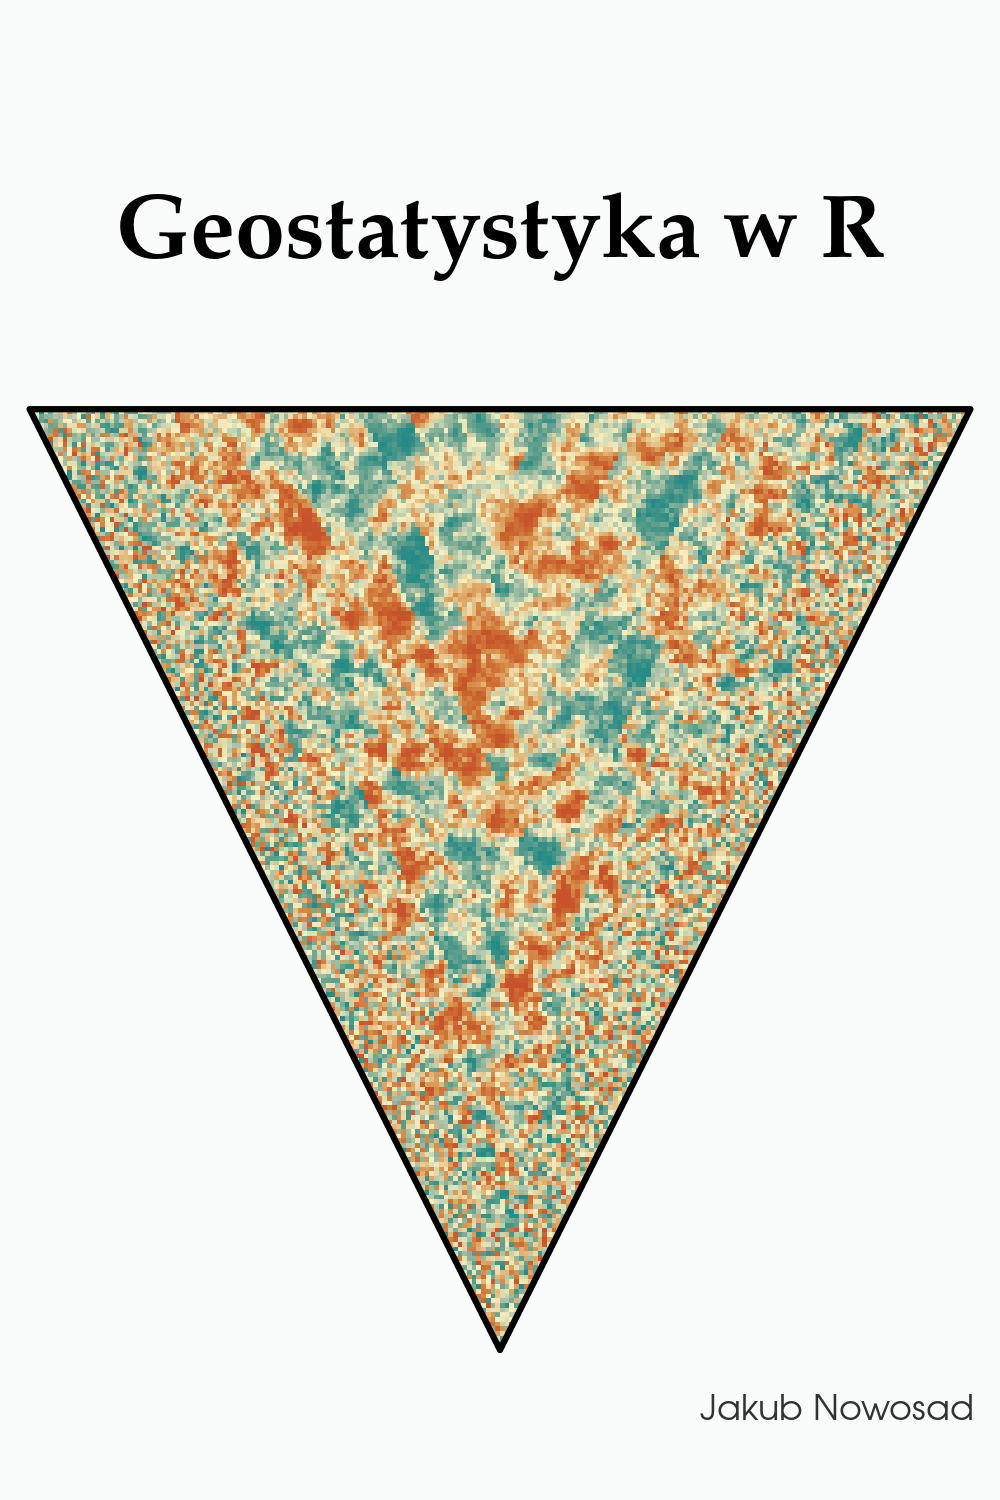
\includepdf{Rfigs/book_cover3.png}

\let\maketitle\oldmaketitle
\maketitle

\thispagestyle{empty}
\vspace*{\fill}
% Wydanie drugie, Poznań 2019 \\
Wydanie trzecie, Poznań 2021 \\
Space A \\
Książka wydana na licencji Creative Commons BY \& SA \\
Więcej informacji \url{https://bookdown.org/nowosad/geostatystyka/} \\
\\
\\
{\large ISBN: 978-83-953296-2-3}



\renewcommand*\contentsname{Spis treści}
{
\setcounter{tocdepth}{2}
\tableofcontents
}
\chapter*{O skrypcie}\label{o-skrypcie}


Masz przed sobą skrypt zawierający materiały do ćwiczeń z geostatystyki.
Składa się ona z kilkunastu rozdziałów pokazujących jak: wygląda geostatystyczna analiza danych (rozdział \ref{wprowadzenie}), dodawać i wizualizować dane przestrzenne w R (rozdział \ref{r-a-dane-przestrzenne}), wykonywać wstępną eksplorację danych nieprzestrzennych (rozdział \ref{eksploracja-analiza-danych-nieprzestrzennych}), wstępnie analizować dane przestrzenne (rozdział \ref{eksploracyjna-analiza-danych-przestrzennych}), wykorzystywać deterministyczne metody interpolacji (rozdział \ref{metody-interpolacji}), rozumieć i wykorzystywać przestrzenne miary podobieństwa i niepodobieństwa (rozdział \ref{geostatystyka-prolog}), modelować semiwariogramy bezkierunkowe i kierunkowe (rozdział \ref{modelowanie-matematycznie-autokorelacji-przestrzennej}), tworzyć estymacje jednozmienne (rozdział \ref{estymacje-jednozmienne}), estymacje wykorzystujące dane uzupełniające (rozdział \ref{wykorzystanie-do-estymacji-danych-uzupeniajacych}), estymacje wielozmienne (rozdział \ref{estymacje-wielozmienne}), estymacje danych kodowanych (rozdział \ref{estymacja-lokalnego-rozkadu-prawdopodobienstwa}), oceniać jakość wykonanych estymacji (rozdział \ref{ocena-jakosci-estymacji}) oraz budować symulacje przestrzenne (rozdział \ref{symulacje}).
Począwszy od drugiego, każdy rozdział kończy się również szeregiem zadań, które pozwalają na sprawdzenie umiejętności i ich utrwalenie.

Dodatkowo załączone są trzy appendiksy.
W appendiksie \ref{zrodla-wiedzy} można znaleźć odnośniki do innych materiałów związanych z geostatystyką i R, appendiks \ref{dane-app} opisuje dane użyte w tym skrypcie, a appendiks \ref{przyklad} pokazuje uproszczony przykład analizy geostatystycznej.

Jest to trzecie wydanie tego skryptu.
Wersje PDF wydania pierwszego i drugiego można znaleźć pod adresem \url{https://jakubnowosad.com/publications}.
Główne zmiany względem drugiego wydania to:

\begin{itemize}
\tightlist
\item
  Przejście ze stosowania pakietu \textbf{sp} na pakiety \textbf{sf} i \textbf{stars}
\item
  Dodanie nowych rycin i poprawienie istniejących
\item
  Dodanie podpisów pod rycinami
\item
  Zaktualizowanie źródeł wiedzy
\item
  Poprawienie sekcji o transformacjach danych
\item
  Dodanie sekcji o rozgrupowaniu danych
\end{itemize}

Wszystkie zaprezentowane metody i analizy zawierają również kod w języku R.
Skrypt został stworzony w R \citep{R-base} z wykorzystaniem pakietów \textbf{bookdown} \citep{R-bookdown}, \textbf{rmarkdown} \citep{R-rmarkdown}, \textbf{knitr} \citep{R-knitr} oraz programu \href{http://pandoc.org/}{Pandoc}.
Aktualna wersja skryptu znajduje się pod adresem \url{https://bookdown.org/nowosad/geostatystyka/}.

Jeżeli używasz skryptu, zacytuj go jako:

\begin{itemize}
\tightlist
\item
  Nowosad, J., (2021). Geostatystyka w R. Poznań: Space A. ISBN 978-83-953296-2-3. Online:
  \url{https://bookdown.org/nowosad/geostatystyka/}
\end{itemize}

Zachęcam do zgłaszania wszelkich uwag, błędów, pomysłów oraz komentarzy na stronie \url{https://github.com/Nowosad/geostat_book/issues}.

Ta książka jest dostępna na licencji Creative Commons Uznanie autorstwa 4.0 Międzynarodowe.

\section*{Wymagania wstępne}\label{wymagania-wstux119pne}


\subsection*{Oprogramowanie}\label{oprogramowanie}


Do odtworzenia przykładów użytych w poniższym skrypcie wystarczy podstawowa znajomość R.
Aby zainstalować R oraz RStudio można skorzystać z poniższych odnośników:

\begin{itemize}
\tightlist
\item
  \href{https://www.r-project.org/}{R} - \url{https://cloud.r-project.org/}
\item
  \href{https://www.rstudio.com/}{RStudio} - \url{https://www.rstudio.com/products/rstudio/download/}
\end{itemize}

Dodatkowo, użyte zostały poniższe pakiety R \citep{R-dismo, R-fields, R-ggplot2, R-gridExtra, R-gstat, R-mapview, R-pgirmess, R-rcartocolor, R-rsample, R-sf, R-stars}.

\begin{Shaded}
\begin{Highlighting}[]
\NormalTok{pakiety }\OtherTok{=} \FunctionTok{c}\NormalTok{(}
  \StringTok{"dismo"}\NormalTok{, }\StringTok{"fields"}\NormalTok{, }\StringTok{"ggplot2"}\NormalTok{, }\StringTok{"gridExtra"}\NormalTok{, }\StringTok{"gstat"}\NormalTok{, }\StringTok{"mapview"}\NormalTok{, }
  \StringTok{"pgirmess"}\NormalTok{, }\StringTok{"rcartocolor"}\NormalTok{, }\StringTok{"rsample"}\NormalTok{, }\StringTok{"sf"}\NormalTok{, }\StringTok{"stars"}\NormalTok{, }\StringTok{"tmap"}
\NormalTok{)}
\end{Highlighting}
\end{Shaded}

Pakiety R używane w tym skrypcie można zainstalować za pomocą metapakietu \textbf{geostatbook} \citep{R-geostatbook}:

\begin{Shaded}
\begin{Highlighting}[]
\FunctionTok{install.packages}\NormalTok{(}\StringTok{"remotes"}\NormalTok{)}
\NormalTok{remotes}\SpecialCharTok{::}\FunctionTok{install\_github}\NormalTok{(}\StringTok{"nowosad/geostatbook@3"}\NormalTok{)}
\end{Highlighting}
\end{Shaded}

\subsection*{Dane}\label{dane}


Dane wykorzystywane w tym skrypcie można pobrać w postaci spakowanego archiwum (dla rozdziału \ref{r-a-dane-przestrzenne}) oraz korzystając z pakietu \textbf{geostatbook} (dla kolejnych rozdziałów).

\begin{itemize}
\tightlist
\item
  \href{https://github.com/Nowosad/geostat_book/blob/master/dane3.zip?raw=true}{Archiwum zawierające dane do rozdziału drugiego}
\item
  \href{https://github.com/Nowosad/geostatbook}{Dane do kolejnych rozdziałów są zawarte w pakiecie geostatbook:}
\end{itemize}

\begin{Shaded}
\begin{Highlighting}[]
\CommentTok{\# install.packages("remotes")}
\NormalTok{remotes}\SpecialCharTok{::}\FunctionTok{install\_github}\NormalTok{(}\StringTok{"nowosad/geostatbook@3"}\NormalTok{)}
\end{Highlighting}
\end{Shaded}

Aby ułatwić korzystanie ze skryptu, rozdziały od \ref{eksploracja-analiza-danych-nieprzestrzennych} do \ref{symulacje} rozpoczynają się od wczytania wymaganych pakietów oraz zbiorów danych.

\chapter{Wprowadzenie}\label{wprowadzenie}

\section{Geostatystyczna analiza danych}\label{geostatystyczna-analiza-danych}

\begin{quote}
Geostatystyka to gałąź statystyki skupiająca się na przestrzennych lub czasoprzestrzennych zbiorach danych
\end{quote}

Geostatystyka jest stosowana obecnie w wielu dyscyplinach, takich jak geologia naftowa, oceanografia, geochemia, logistyka, leśnictwo, gleboznawstwo, hydrologia, meteorologia, czy epidemiologia.

Geostatystyczna analiza danych może przyjmować różną postać w zależności od postawionego celu analizy.
Rycina \ref{fig:01-wprowadzenie-1} przestawia uproszczoną ścieżkę postępowania geostatystycznego.

\begin{figure}

{\centering 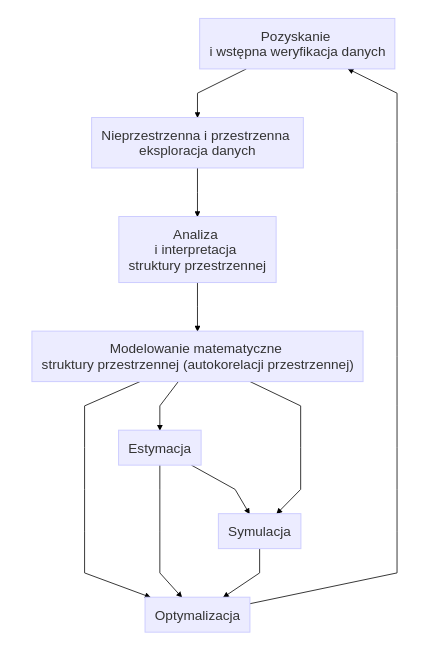
\includegraphics[width=1\linewidth]{figs/diag} 

}

\caption{Uproszczona ścieżka postępowania geostatystycznego.}\label{fig:01-wprowadzenie-1}
\end{figure}

Punktem wyjścia analizy geostatystycznej jest posiadanie danych przestrzennych opisujących badane zjawisko, np. w \textbf{postaci punktowej} (rycina \ref{fig:01-wprowadzenie-3}).

\begin{figure}

{\centering 
\includegraphics[width=1\linewidth]{01-wprowadzenie_files/figure-latex/01-wprowadzenie-3-1} 

}

\caption{Przykładowe dane reprezentujące pomiary punktowe zmiennej numerycznej.}\label{fig:01-wprowadzenie-3}
\end{figure}

Dane należy poddać eksploracji w celu ich lepszego poznania, wyszukania relacji między zmiennymi, czy znalezienia potencjalnych błędów (rycina \ref{fig:01-wprowadzenie-3b}).

\begin{figure}

{\centering 
\includegraphics[width=1\linewidth]{01-wprowadzenie_files/figure-latex/01-wprowadzenie-3b-1} 

}

\caption{Rozkład wartości zmiennej numerycznej.}\label{fig:01-wprowadzenie-3b}
\end{figure}

Na ich podstawie chcemy zrozumieć zmienność przestrzenną analizowanej cechy.
Do tego może nam posłużyć wykres nazywany \textbf{semiwariogramem} (rycina \ref{fig:01-wprowadzenie-4}).

\begin{figure}

{\centering 
\includegraphics[width=1\linewidth]{01-wprowadzenie_files/figure-latex/01-wprowadzenie-4-1} 

}

\caption{Wykres, nazywany semiwariogramem, reprezentujący niepodobieństwo wartości wraz z odległością.}\label{fig:01-wprowadzenie-4}
\end{figure}

\textbf{Semiwariogram} opisuje przestrzenną zmienność badanej cechy i za jego pomocą możemy stwierdzić jak to zjawisko zmienia się w przestrzeni.
Dodatkowo za pomocą \textbf{mapy semiwariogramu} (rycina \ref{fig:01-wprowadzenie-5}) możliwe jest stwierdzenie czy istnieją jakieś kierunki w których ta cecha zmienia się zmienia bardziej dynamicznie, a w których ta zmiana jest wolniejsza.

\begin{figure}

{\centering 
\includegraphics[width=1\linewidth]{01-wprowadzenie_files/figure-latex/01-wprowadzenie-5-1} 

}

\caption{Mapa semiwariogramu reprezentująca niepodobieństwo wartości wraz z odległością i kierunkiem.}\label{fig:01-wprowadzenie-5}
\end{figure}

Następnie korzystając z wiedzy uzyskanej z semiwariogramu i mapy semiwariogramu, jesteśmy w stanie stworzyć \textbf{model semiwariogramu} (rycina \ref{fig:01-wprowadzenie-6}).

\begin{figure}

{\centering 
\includegraphics[width=1\linewidth]{01-wprowadzenie_files/figure-latex/01-wprowadzenie-6-1} 

}

\caption{Model reprezentowany przez ciągłą linię naniesiony na semiwariogram.}\label{fig:01-wprowadzenie-6}
\end{figure}

Pozwala on zarówno na lepszy opis zmienności zjawiska, jak również służy do tworzenia \textbf{estymacji} czy też~\textbf{symulacji}.
Estymacja tworzy najbardziej potencjalnie możliwą wartość dla wybranej lokalizacji (rycina \ref{fig:01-wprowadzenie-7}).

\begin{figure}

{\centering 
\includegraphics[width=1\linewidth]{01-wprowadzenie_files/figure-latex/01-wprowadzenie-7-1} 

}

\caption{Estymacja (oszacowanie) wartości badanej zmiennej dla całego obszaru.}\label{fig:01-wprowadzenie-7}
\end{figure}

Rolą symulacji (rycina \ref{fig:01-wprowadzenie-8}) jest natomiast generowanie równie prawdopodobne możliwości rozkładu badanej cechy.

\begin{figure}

{\centering 
\includegraphics[width=1\linewidth]{01-wprowadzenie_files/figure-latex/01-wprowadzenie-8-1} 

}

\caption{Przykłady symulowanych wartości badanej zmiennej dla całego obszaru.}\label{fig:01-wprowadzenie-8}
\end{figure}

Każdy z powyższych elementów geostatystycznej analizy danych zostanie rozwinięty w dalszych rozdziałach tego skryptu.

\chapter{R a dane przestrzenne}\label{r-a-dane-przestrzenne}

\section{Wprowadzenie}\label{wprowadzenie-1}

\subsection{Reprezentacja danych nieprzestrzennych}\label{reprezentacja-danych-nieprzestrzennych}

Skrypty i funkcje w języku R są zbudowane na podstawie szeregu obiektów nieprzestrzennych.
Do wbudowanych typów obiektów należą:

\begin{itemize}
\tightlist
\item
  Wektory atomowe (ang. \emph{vector}):

  \begin{itemize}
  \tightlist
  \item
    liczbowe (ang. \emph{integer}, \emph{numeric}) - \texttt{c(1,\ 2,\ 3)} i \texttt{c(1.21,\ 3.32,\ 4.43)}
  \item
    znakowe (ang. \emph{character}) - \texttt{c("jeden",\ "dwa",\ "trzy")}
  \item
    logiczne (ang. \emph{logical}) - \texttt{c(TRUE,\ FALSE)}
  \end{itemize}
\item
  Ramki danych (ang. \emph{data.frame}) - to zbiór zmiennych (kolumn) oraz obserwacji (wierszy) zawierających różne typy danych
\item
  Macierze (ang. \emph{matrix}) - to zbiór kolumn oraz wierszy zawierających wektory jednego typu
\item
  Listy (ang. \emph{list}) - to sposób przechowywania obiektów o różnych typach i różnej długości
\end{itemize}

Dokładniejsze wyjaśnienie powyższych typów obiektów można znaleźć w rozdziałach 5 i 7 książki \href{https://nowosad.github.io/elp/}{Elementarz programisty: Wstęp do programowania używając R}.

\subsection{Pakiety}\label{pakiety}

R zawiera także wiele funkcji pozwalających na przetwarzanie, wizualizację i analizowanie danych przestrzennych.
Zawarte są one w szeregu pakietów (zbiorów funkcji), między innymi:

\begin{itemize}
\tightlist
\item
  Obsługa danych przestrzennych - \textbf{sf}, \textbf{stars}, \textbf{terra}, \textbf{raster}, \textbf{sp}
\item
  Geostatystyka - \textbf{gstat}, \textbf{geoR}
\end{itemize}

Więcej szczegółów na ten temat pakietów R służących do analizy przestrzennej można znaleźć pod adresem \url{https://cran.r-project.org/view=Spatial}.

\subsection{Reprezentacja danych przestrzennych}\label{reprezentacja-danych-przestrzennych}

Dane przestrzenne mogą być reprezentowane w R poprzez wiele różnych klas obiektów z użyciem różnych pakietów R.
Przykładowo dane wektorowe mogą być reprezentowane poprzez obiekty klasy \texttt{Spatial*} z pakietu \textbf{sp} oraz obiekty klasy \texttt{sf} z pakietu \textbf{sf}.

Pakiet \textbf{sf} oparty jest o standard OGC o nazwie Simple Features.
Większość jego funkcji zaczyna się od prefiksu \texttt{st\_}.
Ten pakiet definiuje klasę obiektów \texttt{sf}, która jest sposobem reprezentacji przestrzennych danych wektorowych.
Pozwala on na stosowanie dodatkowych typów danych wektorowych (np. poligon i multipoligon to dwie oddzielne klasy), łatwiejsze przetwarzanie danych, oraz obsługę przestrzennych baz danych takich jak PostGIS.
Pakiet \textbf{sf} jest używany przez kilkadziesiąt dodatkowych pakietów R, jednak wiele metod i funkcji nadal wymaga obiektów klasy \textbf{sp}.
Porównanie funkcji dostępnych w pakietach \textbf{sp} i \textbf{sf} można znaleźć pod adresem \url{https://github.com/r-spatial/sf/wiki/Migrating}.
Więcej o pakiecie \textbf{sf} można przeczytać w \href{https://geocompr.robinlovelace.net/spatial-class.html}{rozdziale drugim} książki Geocomputation with R.

Dane rastrowe są reprezentowane między innymi poprzez klasę \texttt{SpatialGridDataFrame} z pakietu \textbf{sp}, obiekty klasy \texttt{Raster*} z pakietu \textbf{raster}, \texttt{SpatRaster} z pakietu \textbf{terra}, oraz klasę \texttt{stars} z pakietu \textbf{stars}.

Pakiet \textbf{stars} (\emph{scalable, spatiotemporal tidy arrays}) pozwala na obsługę różnorodnych danych przestrzennych i czasoprzestrzennych reprezentowanych jako kostka danych (ang. \emph{data cubes}).
Obejmuje to, między innymi, regularne i nieregularne dane rastrowe, ale także czasoprzestrzenne dane wektorowe.
Ten pakiet zapewnia klasy i metody do wczytywania, przetwarzania, wizualizacji czy zapisywania kości danych.
Posiada on także wbudowaną integrację~z pakietem \textbf{sf}.

\subsection{GDAL/OGR}\label{gdalogr}

Pakiety \textbf{sf} czy \textbf{stars} wykorzystują zewnętrzne biblioteki \href{http://www.gdal.org/}{GDAL/OGR} w R do wczytywania i zapisywania danych przestrzennych.
GDAL to biblioteka zawierająca funkcje służące do odczytywania i zapisywania danych w formatach rastrowych, a OGR to biblioteka służąca to odczytywania i zapisywania danych w formatach wektorowych.

\subsection{PROJ}\label{proj}

Dane przestrzenne powinny być zawsze powiązane z układem współrzędnych - w ten sposób możliwe jest określenie gdzie są one położone, a także jak wykonywane są na nich operacje przestrzenne.
Biblioteka \href{https://proj.org/}{PROJ} jest używana przez pakiety \textbf{sf} i \textbf{stars} do określania i konwersji układów współrzędnych.
Układy współrzędnych mogą być opisywane na szereg sposobów, np. poprzez systemy kodów.
Najpopularniejszym z nich jest system kodów EPSG (ang. \emph{European Petroleum Survey Group}), który pozwala on na łatwe identyfikowanie układów współrzędnych.
Przykładowo, układ PL 1992 może być określony jako \texttt{"EPSG:2180"}.
Taki sposób określania układów współrzędnych wymaga jedynie znajomości odpowiedniego numery dla danego obszaru.

Dane przestrzenne przechowują też opis tego układu współrzędnych w bardziej złożony sposób nazwany WKT2.
Zawiera on opis elementów związanych z konkretnym układem współrzędnych, takich jak jednostka, elipsoida odwzorowania, itd.

Warto też wiedzieć, że przez wiele lat główną rolę pełniła reprezentacja \textbf{proj4string}, np. \texttt{"+proj=tmerc\ +lat\_0=0\ +lon\_0=19\ +k=0.9993\ +x\_0=500000\ +y\_0=-5300000\ +ellps=GRS80\ +towgs84=0,0,0,0,0,0,0\ +units=m\ +no\_defs"}, która określała własności układu współrzędnych.
Współcześnie jednak ta reprezentacja nie jest zalecana do użycia.

Strona \url{https://epsg.org/} zawiera bazę danych układów współrzędnych.

\subsection{Układy współrzędnych}\label{ukux142ady-wspuxf3ux142rzux119dnych}

Dane przestrzenne mogą być reprezentowane używając układów współrzędnych geograficznych lub prostokątnych płaskich.

W układzie współrzędnych geograficznych proporcje pomiędzy współrzędną oznaczającą długość geograficzną (X) a oznaczającą szerokość geograficzną (Y) nie są równe 1:1.
Realna wielkość oczka siatki (jego powierzchnia) jest zmienna, a jednostka mapy jest abstrakcyjna w tych układach.
W efekcie nie pozwala to na proste określanie odległości czy powierzchni.
Powyższe cechy układów współrzędnych geograficznych powodują, że do większości algorytmów w geostatystyce wykorzystywane są układy współrzędnych prostokątnych płaskich.

Układy współrzędnych prostokątnych płaskich określane są w miarach liniowych (np. metrach).
W tych układach proporcje między współrzędną X a Y są równe 1:1, a wielkość oczka jest stała.

\subsection{GEOS}\label{geos}

Pakiet \textbf{sf} używa biblioteki \href{https://libgeos.org/}{GEOS} do wykonywania operacji przestrzennych.
Przykładowe funkcje tej biblioteki to tworzenie buforów, wyliczanie centroidów, określanie relacji topologicznych (np. przecina, zawiera, etc.) i wiele innych.

\section{Import danych}\label{import-danych}

R pozwala na odczytywanie danych przestrzennych z wielu formatów.
Do najpopularniejszych należą dane tekstowe z plików o rozszerzeniu \texttt{.csv}, dane wektorowe z plików \texttt{.shp}, dane rastrowe z plików w formacie GeoTIFF, oraz bazy danych przestrzennych z plików rozszerzeniu \texttt{.gpkg}.

\subsection{Format .csv (dane punktowe)}\label{format-.csv-dane-punktowe}

Dane z plików tekstowych (np. rozszerzenie \texttt{.csv}) można odczytać za pomocą uogólnionej funkcji \texttt{read.table()} lub też funkcji szczegółowych - \texttt{read.csv()} lub \texttt{read.csv2()}.

\begin{Shaded}
\begin{Highlighting}[]
\NormalTok{dane\_punktowe }\OtherTok{=} \FunctionTok{read.csv}\NormalTok{(}\StringTok{"dane/punkty.csv"}\NormalTok{)}
\end{Highlighting}
\end{Shaded}

\begin{Shaded}
\begin{Highlighting}[]
\FunctionTok{head}\NormalTok{(dane\_punktowe)}
\end{Highlighting}
\end{Shaded}

\begin{verbatim}
##       srtm clc      temp      ndvi      savi        x        y
## 1 175.7430   1 13.852222 0.6158061 0.4189449 750298.0 716731.6
## 2 149.8111   1 15.484209 0.5558816 0.3794864 753482.9 717331.4
## 3 272.8583  NA 12.760814 0.6067462 0.3745572 747242.5 720589.0
## 4 187.2777   1 14.324648 0.3756170 0.2386246 755798.9 718828.1
## 5 260.1366   1 15.908549 0.4598393 0.3087599 746963.5 717533.5
## 6 160.1416   2  9.941118 0.5600288 0.3453627 756801.6 720474.1
\end{verbatim}

Po wczytaniu za pomocą funkcji \texttt{read.csv()}, nowy obiekt (np. \texttt{dane\_punktowe}) jest reprezentowany za pomocą klasy nieprzestrzennej \texttt{data.frame}.
Aby obiekt został przetworzony do klasy przestrzennej, konieczne jest określenie które kolumny zawierają informacje o współrzędnych; w tym wypadku współrzędne znajduję się w kolumnach \texttt{x} oraz \texttt{y}.
Nadanie układu współrzędnych odbywa się poprzez funkcję \texttt{st\_as\_sf()}.

\begin{Shaded}
\begin{Highlighting}[]
\FunctionTok{library}\NormalTok{(sf)}
\NormalTok{dane\_punktowe\_sf }\OtherTok{=} \FunctionTok{st\_as\_sf}\NormalTok{(dane\_punktowe, }\AttributeTok{coords =} \FunctionTok{c}\NormalTok{(}\StringTok{"x"}\NormalTok{, }\StringTok{"y"}\NormalTok{))}
\NormalTok{dane\_punktowe\_sf}
\end{Highlighting}
\end{Shaded}

\begin{verbatim}
## Simple feature collection with 248 features and 5 fields
## Geometry type: POINT
## Dimension:     XY
## Bounding box:  xmin: 745592.5 ymin: 712642.4 xmax: 756967.8 ymax: 721238.7
## CRS:           NA
## First 10 features:
##        srtm clc      temp      ndvi      savi                  geometry
## 1  175.7430   1 13.852222 0.6158061 0.4189449   POINT (750298 716731.6)
## 2  149.8111   1 15.484209 0.5558816 0.3794864 POINT (753482.9 717331.4)
## 3  272.8583  NA 12.760814 0.6067462 0.3745572   POINT (747242.5 720589)
## 4  187.2777   1 14.324648 0.3756170 0.2386246 POINT (755798.9 718828.1)
## 5  260.1366   1 15.908549 0.4598393 0.3087599 POINT (746963.5 717533.5)
## 6  160.1416   2  9.941118 0.5600288 0.3453627 POINT (756801.6 720474.1)
## 7  192.9223   2 13.514751 0.6009588 0.3737249   POINT (752698 718623.6)
## 8  234.9989   1 12.919225 0.4979195 0.2978503 POINT (749399.8 716955.2)
## 9  228.7312   1 19.247132 0.3819634 0.2077981   POINT (748766.6 713889)
## 10 240.5474   2 10.529105 0.5795159 0.3805268   POINT (749290.4 718861)
\end{verbatim}

Ważne, ale nie wymagane, jest także dodanie informacji o układzie przestrzennym danych za pomocą funkcji \texttt{st\_set\_crs()}.

\begin{Shaded}
\begin{Highlighting}[]
\NormalTok{dane\_punktowe\_sf }\OtherTok{=} \FunctionTok{st\_set\_crs}\NormalTok{(dane\_punktowe\_sf, }\AttributeTok{value =} \StringTok{"EPSG:2180"}\NormalTok{)}
\end{Highlighting}
\end{Shaded}

Proste wizualizacje uzyskanych danych klasy przestrzennej, np. \texttt{sf} czy \texttt{stars}, można uzyskać za pomocą funkcji \texttt{plot()} (rycina \ref{fig:02-r-a-dane-przestrzenne-5} i \ref{fig:02-r-a-dane-przestrzenne-7a}).

\begin{Shaded}
\begin{Highlighting}[]
\FunctionTok{plot}\NormalTok{(dane\_punktowe\_sf)}
\end{Highlighting}
\end{Shaded}

\begin{figure}

{\centering 
\includegraphics[width=1\linewidth]{02-r-a-dane-przestrzenne_files/figure-latex/02-r-a-dane-przestrzenne-5-1} 

}

\caption{Efekt działania funkcji plot na obiekcie klasy sf.}\label{fig:02-r-a-dane-przestrzenne-5}
\end{figure}

\subsection{Dane wektorowe}\label{dane-wektorowe}

Dane wektorowe (np. w formacie GeoPackage czy ESRI Shapefile) można odczytać za pomocą funkcji \texttt{read\_sf()} z pakietu \textbf{sf}.
Przyjmuje ona co najmniej jeden argument - \texttt{dsn}, który określa główny plik w którym znajdują się dane.

\begin{Shaded}
\begin{Highlighting}[]
\FunctionTok{library}\NormalTok{(sf)}
\NormalTok{granica\_sf }\OtherTok{=} \FunctionTok{read\_sf}\NormalTok{(}\AttributeTok{dsn =} \StringTok{"dane/granica.gpkg"}\NormalTok{)}
\CommentTok{\# plot(granica\_sf)}
\end{Highlighting}
\end{Shaded}

\subsection{Dane rastrowe}\label{dane-rastrowe}

Istnieje kilka sposobów odczytu danych rastrowych w R.
Do najpopularniejszych należą funkcje \texttt{rast()} z pakietu \textbf{terra} i \texttt{raster()} z pakietu \textbf{raster}.
W poniższym przykładzie użyjemy funkcji \texttt{read\_stars()} z pakietu \textbf{stars}.
Należy w niej jedynie podać ścieżkę do pliku rastrowego.

\begin{Shaded}
\begin{Highlighting}[]
\FunctionTok{library}\NormalTok{(stars)}
\NormalTok{siatka\_stars }\OtherTok{=} \FunctionTok{read\_stars}\NormalTok{(}\StringTok{"dane/siatka.tif"}\NormalTok{)}
\NormalTok{siatka\_stars}
\end{Highlighting}
\end{Shaded}

\begin{verbatim}
## stars object with 2 dimensions and 1 attribute
## attribute(s):
##             Min. 1st Qu. Median Mean 3rd Qu. Max. NA's
## siatka.tif     0       0      0    0       0    0 1270
## dimension(s):
##   from  to offset delta             refsys point x/y
## x    1 127 745542    90 ETRF2000-PL / CS92 FALSE [x]
## y    1  96 721256   -90 ETRF2000-PL / CS92 FALSE [y]
\end{verbatim}

\begin{Shaded}
\begin{Highlighting}[]
\FunctionTok{plot}\NormalTok{(siatka\_stars)}
\end{Highlighting}
\end{Shaded}

\begin{figure}

{\centering 
\includegraphics[width=1\linewidth]{02-r-a-dane-przestrzenne_files/figure-latex/02-r-a-dane-przestrzenne-7a-1} 

}

\caption{Efekt działania funkcji plot na obiekcie klasy sf.}\label{fig:02-r-a-dane-przestrzenne-7a}
\end{figure}

\section{Przeglądanie danych przestrzennych}\label{przeglux105danie-danych-przestrzennych}

\subsection{Struktura obiektu}\label{struktura-obiektu}

Podstawowe informacje o obiekcie można uzyskać poprzez wpisanie jego nazwy:

\begin{Shaded}
\begin{Highlighting}[]
\NormalTok{dane\_punktowe\_sf}
\end{Highlighting}
\end{Shaded}

\begin{verbatim}
## Simple feature collection with 248 features and 5 fields
## Geometry type: POINT
## Dimension:     XY
## Bounding box:  xmin: 745592.5 ymin: 712642.4 xmax: 756967.8 ymax: 721238.7
## Projected CRS: ETRF2000-PL / CS92
## First 10 features:
##        srtm clc      temp      ndvi      savi                  geometry
## 1  175.7430   1 13.852222 0.6158061 0.4189449   POINT (750298 716731.6)
## 2  149.8111   1 15.484209 0.5558816 0.3794864 POINT (753482.9 717331.4)
## 3  272.8583  NA 12.760814 0.6067462 0.3745572   POINT (747242.5 720589)
## 4  187.2777   1 14.324648 0.3756170 0.2386246 POINT (755798.9 718828.1)
## 5  260.1366   1 15.908549 0.4598393 0.3087599 POINT (746963.5 717533.5)
## 6  160.1416   2  9.941118 0.5600288 0.3453627 POINT (756801.6 720474.1)
## 7  192.9223   2 13.514751 0.6009588 0.3737249   POINT (752698 718623.6)
## 8  234.9989   1 12.919225 0.4979195 0.2978503 POINT (749399.8 716955.2)
## 9  228.7312   1 19.247132 0.3819634 0.2077981   POINT (748766.6 713889)
## 10 240.5474   2 10.529105 0.5795159 0.3805268   POINT (749290.4 718861)
\end{verbatim}

Obiekty \texttt{sf} są~zbudowane z tabeli (\emph{data frame}) wraz z dodatkową~kolumną zawierającą~geometrie (często nazywaną \texttt{geometry} lub \texttt{geom}) oraz szeregu atrybutów przestrzennych.
Strukturę obiektu \texttt{sf} można sprawdzić za pomocą funkcji \texttt{str()}:

\begin{Shaded}
\begin{Highlighting}[]
\FunctionTok{str}\NormalTok{(dane\_punktowe\_sf)}
\end{Highlighting}
\end{Shaded}

\begin{verbatim}
## Classes 'sf' and 'data.frame':   248 obs. of  6 variables:
##  $ srtm    : num  176 150 273 187 260 ...
##  $ clc     : int  1 1 NA 1 1 2 2 1 1 2 ...
##  $ temp    : num  13.9 15.5 12.8 14.3 15.9 ...
##  $ ndvi    : num  0.616 0.556 0.607 0.376 0.46 ...
##  $ savi    : num  0.419 0.379 0.375 0.239 0.309 ...
##  $ geometry:sfc_POINT of length 248; first list element:  'XY' num  750298 716732
##  - attr(*, "sf_column")= chr "geometry"
##  - attr(*, "agr")= Factor w/ 3 levels "constant","aggregate",..: NA NA NA NA NA
##   ..- attr(*, "names")= chr [1:5] "srtm" "clc" "temp" "ndvi" ...
\end{verbatim}

Obiekty \texttt{stars} mogą przyjmować różną formę w zależności od tego czy reprezentują one dane wektorowe czy rastrowe oraz tego ile wymiarów posiadają te dane.
Przykładowy obiekt \texttt{siatka\_stars} posiada dwa wymiary (\texttt{x} i \texttt{y}) oraz jeden atrybut (\texttt{siatka.tif}).

\begin{Shaded}
\begin{Highlighting}[]
\NormalTok{siatka\_stars}
\end{Highlighting}
\end{Shaded}

\begin{verbatim}
## stars object with 2 dimensions and 1 attribute
## attribute(s):
##             Min. 1st Qu. Median Mean 3rd Qu. Max. NA's
## siatka.tif     0       0      0    0       0    0 1270
## dimension(s):
##   from  to offset delta             refsys point x/y
## x    1 127 745542    90 ETRF2000-PL / CS92 FALSE [x]
## y    1  96 721256   -90 ETRF2000-PL / CS92 FALSE [y]
\end{verbatim}

Jest on zbudowany jako lista zawierająca dwuwymiarową macierz wraz ze zbiorem metadanych (można to sprawdzić za pomocą funkcji \texttt{str(siatka\_stars)}).

\subsection{Tabla atrybutów}\label{tabla-atrybutuxf3w}

Funkcja \texttt{st\_drop\_geometry()} pozwala na pozbycie się~informacji przestrzennych z obiektu klasy \texttt{sf} i uzyskanie jedynie obiektu klasy \texttt{data.frame} zawierającego nieprzestrzenne informacje o kolejnych punktach w tym zbiorze.

\begin{Shaded}
\begin{Highlighting}[]
\NormalTok{punkty\_df }\OtherTok{=} \FunctionTok{st\_drop\_geometry}\NormalTok{(dane\_punktowe\_sf)}
\FunctionTok{head}\NormalTok{(punkty\_df)}
\end{Highlighting}
\end{Shaded}

\begin{verbatim}
##       srtm clc      temp      ndvi      savi
## 1 175.7430   1 13.852222 0.6158061 0.4189449
## 2 149.8111   1 15.484209 0.5558816 0.3794864
## 3 272.8583  NA 12.760814 0.6067462 0.3745572
## 4 187.2777   1 14.324648 0.3756170 0.2386246
## 5 260.1366   1 15.908549 0.4598393 0.3087599
## 6 160.1416   2  9.941118 0.5600288 0.3453627
\end{verbatim}

Przetworzenie obiektu klasy \texttt{stars} na \texttt{data.frame} odbywa się~natomiast używając funkcji \texttt{as.data.frame()}.

\begin{Shaded}
\begin{Highlighting}[]
\NormalTok{siatka\_df }\OtherTok{=} \FunctionTok{as.data.frame}\NormalTok{(siatka\_stars)}
\FunctionTok{head}\NormalTok{(siatka\_df)}
\end{Highlighting}
\end{Shaded}

\begin{verbatim}
##          x        y siatka.tif
## 1 745586.7 721211.2         NA
## 2 745676.7 721211.2         NA
## 3 745766.7 721211.2         NA
## 4 745856.7 721211.2         NA
## 5 745946.7 721211.2         NA
## 6 746036.7 721211.2         NA
\end{verbatim}

\subsection{Współrzędne}\label{wspuxf3ux142rzux119dne}

Funkcja \texttt{st\_coordinates()} pozwala na wydobycie współrzędnych zarówno z obiektu punktowego klasy \texttt{sf} jak i siatki klasy \texttt{stars}.

\begin{Shaded}
\begin{Highlighting}[]
\CommentTok{\# sf}
\NormalTok{xy }\OtherTok{=} \FunctionTok{st\_coordinates}\NormalTok{(dane\_punktowe\_sf)}
\FunctionTok{head}\NormalTok{(xy)}
\end{Highlighting}
\end{Shaded}

\begin{verbatim}
##             X        Y
## [1,] 750298.0 716731.6
## [2,] 753482.9 717331.4
## [3,] 747242.5 720589.0
## [4,] 755798.9 718828.1
## [5,] 746963.5 717533.5
## [6,] 756801.6 720474.1
\end{verbatim}

\begin{Shaded}
\begin{Highlighting}[]
\CommentTok{\# stars}
\NormalTok{siatka\_xy }\OtherTok{=} \FunctionTok{st\_coordinates}\NormalTok{(siatka\_stars)}
\FunctionTok{head}\NormalTok{(siatka\_xy)}
\end{Highlighting}
\end{Shaded}

\begin{verbatim}
##          x        y
## 1 745586.7 721211.2
## 2 745676.7 721211.2
## 3 745766.7 721211.2
## 4 745856.7 721211.2
## 5 745946.7 721211.2
## 6 746036.7 721211.2
\end{verbatim}

\subsection{Obwiednia}\label{obwiednia}

Funkcja \texttt{st\_bbox()} określa zasięg przestrzenny danych w jednostkach mapy.

\begin{Shaded}
\begin{Highlighting}[]
\FunctionTok{st\_bbox}\NormalTok{(dane\_punktowe\_sf)}
\end{Highlighting}
\end{Shaded}

\begin{verbatim}
##     xmin     ymin     xmax     ymax 
## 745592.5 712642.4 756967.8 721238.7
\end{verbatim}

\subsection{Układ współrzędnych}\label{ukux142ad-wspuxf3ux142rzux119dnych}

Funkcja \texttt{st\_crs()} wyświetla definicję układu współrzędnych.

\begin{Shaded}
\begin{Highlighting}[]
\FunctionTok{st\_crs}\NormalTok{(dane\_punktowe\_sf)}
\end{Highlighting}
\end{Shaded}

\begin{verbatim}
## Coordinate Reference System:
##   User input: EPSG:2180 
##   wkt:
## PROJCRS["ETRF2000-PL / CS92",
##     BASEGEOGCRS["ETRF2000-PL",
##         DATUM["ETRF2000 Poland",
##             ELLIPSOID["GRS 1980",6378137,298.257222101,
##                 LENGTHUNIT["metre",1]]],
##         PRIMEM["Greenwich",0,
##             ANGLEUNIT["degree",0.0174532925199433]],
##         ID["EPSG",9702]],
##     CONVERSION["Poland CS92",
##         METHOD["Transverse Mercator",
##             ID["EPSG",9807]],
##         PARAMETER["Latitude of natural origin",0,
##             ANGLEUNIT["degree",0.0174532925199433],
##             ID["EPSG",8801]],
##         PARAMETER["Longitude of natural origin",19,
##             ANGLEUNIT["degree",0.0174532925199433],
##             ID["EPSG",8802]],
##         PARAMETER["Scale factor at natural origin",0.9993,
##             SCALEUNIT["unity",1],
##             ID["EPSG",8805]],
##         PARAMETER["False easting",500000,
##             LENGTHUNIT["metre",1],
##             ID["EPSG",8806]],
##         PARAMETER["False northing",-5300000,
##             LENGTHUNIT["metre",1],
##             ID["EPSG",8807]]],
##     CS[Cartesian,2],
##         AXIS["northing (x)",north,
##             ORDER[1],
##             LENGTHUNIT["metre",1]],
##         AXIS["easting (y)",east,
##             ORDER[2],
##             LENGTHUNIT["metre",1]],
##     USAGE[
##         SCOPE["Topographic mapping (medium and small scale)."],
##         AREA["Poland - onshore and offshore."],
##         BBOX[49,14.14,55.93,24.15]],
##     ID["EPSG",2180]]
\end{verbatim}

\section{Przetwarzanie danych przestrzennych}\label{przetwarzanie-danych-przestrzennych}

\subsection{Łączenie danych rastrowych}\label{ux142ux105czenie-danych-rastrowych}

Połączenie danych rastrowych pochodzących z kilku plików może odbyć się~poprzez wczytanie ich jako osobnych obiektów klasy \texttt{stars} a następnie połączenie ich używając funkcji \texttt{c()}.

\begin{Shaded}
\begin{Highlighting}[]
\NormalTok{srtm\_stars }\OtherTok{=} \FunctionTok{read\_stars}\NormalTok{(}\StringTok{"dane/srtm.tif"}\NormalTok{)}
\NormalTok{clc\_stars }\OtherTok{=} \FunctionTok{read\_stars}\NormalTok{(}\StringTok{"dane/clc.tif"}\NormalTok{)}
\NormalTok{dwie\_stars }\OtherTok{=} \FunctionTok{c}\NormalTok{(srtm\_stars, clc\_stars)}
\end{Highlighting}
\end{Shaded}

W efekcie uzyskiwany jest obiekt posiadający dwa atrybuty odpowiadające wczytanym plikom.

\begin{Shaded}
\begin{Highlighting}[]
\NormalTok{dwie\_stars}
\end{Highlighting}
\end{Shaded}

\begin{verbatim}
## stars object with 2 dimensions and 2 attributes
## attribute(s):
##               Min.  1st Qu.   Median      Mean  3rd Qu.     Max. NA's
## srtm.tif  143.6559 186.4765 216.4929 212.21245 235.2941 288.8382 1242
## clc.tif     1.0000   1.0000   1.0000   1.42126   2.0000   4.0000 1270
## dimension(s):
##   from  to offset delta             refsys point x/y
## x    1 127 745542    90 ETRF2000-PL / CS92 FALSE [x]
## y    1  96 721256   -90 ETRF2000-PL / CS92 FALSE [y]
\end{verbatim}

\subsection{Wydobywanie wartości z rastra}\label{wydobywanie-wartoux15bci-z-rastra}

Posiadając dwa obiekty, jeden punktowy a drugi rastrowy, dotyczące tego samego obszaru możliwe jest wydobycie wartości dla punktów używając funkcji \texttt{st\_join()}.

\begin{Shaded}
\begin{Highlighting}[]
\NormalTok{dane\_punktowe\_sf2 }\OtherTok{=} \FunctionTok{st\_join}\NormalTok{(dane\_punktowe\_sf, }\FunctionTok{st\_as\_sf}\NormalTok{(dwie\_stars))}
\end{Highlighting}
\end{Shaded}

\section{Eksport danych}\label{eksport-danych}

\subsection{Zapisywanie danych wektorowych}\label{zapisywanie-danych-wektorowych}

R pozwala również na zapisywanie danych przestrzennych.
W przypadku zapisu danych wektorowych za pomocą funkcji \texttt{write\_sf()} konieczne jest podanie ścieżki i nazwy zapisywanego obiektu wraz z rozszerzeniem (np. \texttt{dane/granica.gpkg}).

\begin{Shaded}
\begin{Highlighting}[]
\FunctionTok{write\_sf}\NormalTok{(granica\_sf, }\AttributeTok{dsn =} \StringTok{"dane/granica.gpkg"}\NormalTok{)}
\end{Highlighting}
\end{Shaded}

\subsection{Zapisywanie danych rastrowych}\label{zapisywanie-danych-rastrowych}

Funkcja \texttt{write\_sf()} pozwala również na zapisywanie danych rastrowych.
Wymaga ona podania dwóch argumentów - nazwy zapisywanego obiektu (np. \texttt{siatka\_stars}) oraz ścieżki i nazwy nowego pliku wraz z rozszerzeniem (np. \texttt{dane/nowa\_siatka.tif}).

\begin{Shaded}
\begin{Highlighting}[]
\FunctionTok{write\_stars}\NormalTok{(siatka\_stars, }\AttributeTok{dsn =} \StringTok{"dane/nowa\_siatka.tif"}\NormalTok{)}
\end{Highlighting}
\end{Shaded}

\section{Wizualizacja danych 2D}\label{wizualizacja-danych-2d}

Do wizualizacji danych przestrzennych w R służy co najmniej kilkanaście różnych pakietów.
Poniżej pokazane są przykłady użycia pakietu \textbf{tmap}.

Poniższy blok kodu tworzy złożoną wizualizację przestrzenną (rycina \ref{fig:02-r-a-dane-przestrzenne-1-bis}) składającą się~z cyfrowego modelu wysokościowego, którego różne wartości są oddane poprzez kolejne kolory (\texttt{tm\_raster()}) i legendę z prawej strony (\texttt{tm\_layout()}); granic Suwalskiego Parku Krajobrazowego (\texttt{tm\_borders()}); kropek przedstawiających dane punktowe (\texttt{tm\_dots()}); podziałki liniowej (\texttt{tm\_scale\_bar()}); strzałki północy (\texttt{tm\_compass}).

\begin{Shaded}
\begin{Highlighting}[]
\FunctionTok{library}\NormalTok{(tmap)}
\FunctionTok{tm\_shape}\NormalTok{(dwie\_stars) }\SpecialCharTok{+}
        \FunctionTok{tm\_raster}\NormalTok{(}\StringTok{"srtm.tif"}\NormalTok{, }\AttributeTok{style =} \StringTok{"cont"}\NormalTok{, }\AttributeTok{title =} \StringTok{"[m npm]"}\NormalTok{) }\SpecialCharTok{+}
        \FunctionTok{tm\_shape}\NormalTok{(granica\_sf) }\SpecialCharTok{+}
        \FunctionTok{tm\_borders}\NormalTok{() }\SpecialCharTok{+}
        \FunctionTok{tm\_shape}\NormalTok{(dane\_punktowe\_sf) }\SpecialCharTok{+}
        \FunctionTok{tm\_dots}\NormalTok{() }\SpecialCharTok{+}
        \FunctionTok{tm\_scale\_bar}\NormalTok{() }\SpecialCharTok{+}
        \FunctionTok{tm\_compass}\NormalTok{(}\AttributeTok{position =} \FunctionTok{c}\NormalTok{(}\StringTok{"left"}\NormalTok{, }\StringTok{"top"}\NormalTok{)) }\SpecialCharTok{+}
        \FunctionTok{tm\_layout}\NormalTok{(}\AttributeTok{legend.outside =} \ConstantTok{TRUE}\NormalTok{)}
\end{Highlighting}
\end{Shaded}

\begin{figure}

{\centering 
\includegraphics[width=1\linewidth]{02-r-a-dane-przestrzenne_files/figure-latex/02-r-a-dane-przestrzenne-1-bis-1} 

}

\caption{Przykład wizualizacji danych 2D stworzonej z użyciem pakietu tmap.}\label{fig:02-r-a-dane-przestrzenne-1-bis}
\end{figure}

Główna idea stojąca za pakietem \textbf{tmap} mówi o łączeniu kolejnych linii kodu znakiem \texttt{+}, i te kolejne elementy będą wyświetlane po sobie.
Podstawową funkcją tego pakietu jest \texttt{tm\_shape()}, która pozwala na zdefiniowanie jaki obiekt przestrzenny chcemy zwizualizować.
Następnie, w zależności od tego jakiego rodzaju jest nasz obiekt (np. czy to punkt czy raster), możemy zdefiniować różne typy wizualizacji.
Dla danych punktowych może to być~\texttt{tm\_dots()} czy \texttt{tm\_symbols()}, dla poligonów - \texttt{tm\_borders()} czy \texttt{tm\_polygons()}, a dla rastrów - \texttt{tm\_raster()}.
Każda z powyższych funkcji jest też~łatwo modyfikowalna, pozwalając na wybranie zmiennej do przestawienia na mapie, stylu legendy, jej tytułu, itd.
Dodatkowo, \textbf{tmap} daje możliwość umieszczenia innych elementów map, takich jak podziałka liniowa (\texttt{tm\_scale\_bar()}) i strzałka północy (\texttt{tm\_compass}).

Więcej o wizualizacji danych przestrzennych można przeczytać w książce \href{https://r-tmap.github.io/tmap-book/}{Elegant and informative maps with tmap} oraz rozdziale \href{https://geocompr.robinlovelace.net/adv-map.html}{Making maps with R} książki Geocomputation with R.

\subsection{Dane punktowe}\label{dane-punktowe}

Pakiet \textbf{tmap} posiada szereg funkcji dla różnych typów danych wejściowych.
W przypadku danych punktowych, najczęściej używane są~\texttt{tm\_symbols()} i \texttt{tm\_dots()}.
Gdy są one używane bez podania dodatkowych argumentów, wówczas otrzymujemy jedynie wizualizację~geometrii naszych danych (rycina \ref{fig:02-r-a-dane-przestrzenne-2-bis}).

\begin{Shaded}
\begin{Highlighting}[]
\FunctionTok{tm\_shape}\NormalTok{(dane\_punktowe\_sf) }\SpecialCharTok{+}
        \FunctionTok{tm\_symbols}\NormalTok{()}
\end{Highlighting}
\end{Shaded}

\begin{figure}

{\centering 
\includegraphics[width=1\linewidth]{02-r-a-dane-przestrzenne_files/figure-latex/02-r-a-dane-przestrzenne-2-bis-1} 

}

\caption{Użycie pakietu plot do wyświetlenia geometrii obiektu klasy sf.}\label{fig:02-r-a-dane-przestrzenne-2-bis}
\end{figure}

Kiedy jednak chcemy przedstawić konkretną zmienną, musimy zadeklarować w jaki sposób ma być~przedstawiona, przykładowo \texttt{col\ =\ "temp"} pokoloruje nasze punkty w zależności od wartości zmiennej \texttt{"temp"} i automatycznie doda odpowiednią legendę.
W takiej sytuacji możemy dodatkowo, np. dodać tytuł legendy (\texttt{title.col\ =\ "Temperatura\ {[}*C{]}")}) czy sposób opisu brakujących wartości \texttt{textNA\ =\ "Brak\ danych"} (rycina \ref{fig:02-r-a-dane-przestrzenne-3-bis}).

\begin{Shaded}
\begin{Highlighting}[]
\FunctionTok{tm\_shape}\NormalTok{(dane\_punktowe\_sf) }\SpecialCharTok{+}
        \FunctionTok{tm\_symbols}\NormalTok{(}\AttributeTok{col =} \StringTok{"temp"}\NormalTok{, }
                   \AttributeTok{title.col =} \StringTok{"Temperatura [*C]"}\NormalTok{,}
                   \AttributeTok{textNA =} \StringTok{"Brak danych"}\NormalTok{)}
\end{Highlighting}
\end{Shaded}

\begin{figure}

{\centering 
\includegraphics[width=1\linewidth]{02-r-a-dane-przestrzenne_files/figure-latex/02-r-a-dane-przestrzenne-3-bis-1} 

}

\caption{Użycie pakietu tmap do wizualizacji zmiennej temp w danych punktowych.}\label{fig:02-r-a-dane-przestrzenne-3-bis}
\end{figure}

Inne możliwe modyfikacje obejmują zmianę~domyślnej palety kolorystycznej (\texttt{palette\ =\ "-Spectral"}) czy też tego w jaki sposób kolejne wartości są przedstawiane (rycina \ref{fig:02-r-a-dane-przestrzenne-4-bis}).
Automatycznie używany jest podział wartości na kilka równych przedziałów, ale możliwe są~również inne podejścia do tego zadania.
Przykładowo, \texttt{style\ =\ "cont"} tworzy ciągłą legendę.

\begin{Shaded}
\begin{Highlighting}[]
\FunctionTok{tm\_shape}\NormalTok{(dane\_punktowe\_sf) }\SpecialCharTok{+}
        \FunctionTok{tm\_symbols}\NormalTok{(}\AttributeTok{col =} \StringTok{"temp"}\NormalTok{, }
                   \AttributeTok{title.col =} \StringTok{"Temperatura [*C]"}\NormalTok{,}
                   \AttributeTok{textNA =} \StringTok{"Brak danych"}\NormalTok{,  }
                   \AttributeTok{palette =} \StringTok{"{-}Spectral"}\NormalTok{,}
                   \AttributeTok{style =} \StringTok{"cont"}\NormalTok{)}
\end{Highlighting}
\end{Shaded}

\begin{figure}

{\centering 
\includegraphics[width=1\linewidth]{02-r-a-dane-przestrzenne_files/figure-latex/02-r-a-dane-przestrzenne-4-bis-1} 

}

\caption{Bardziej złożone zastosowanie pakietu tmap do wizualizacji zmiennej temp w danych punktowych.}\label{fig:02-r-a-dane-przestrzenne-4-bis}
\end{figure}

\subsection{Dane punktowe - kategorie}\label{dane-punktowe---kategorie}

Nie zawsze dane mają postać ciągłych wartości - bywają one również określeniami różnych klas.
W takich sytuacjach należy wcześniej przetworzyć typ danych do postaci kategoryzowanej (\texttt{as.factor()}) lub zmienić sposób przedstawiana wartości na \texttt{"cat"} (rycina \ref{fig:02-r-a-dane-przestrzenne-5-bis}).

\begin{Shaded}
\begin{Highlighting}[]
\FunctionTok{tm\_shape}\NormalTok{(dane\_punktowe\_sf) }\SpecialCharTok{+}
        \FunctionTok{tm\_symbols}\NormalTok{(}\AttributeTok{col =} \StringTok{"clc"}\NormalTok{, }
                   \AttributeTok{title.col =} \StringTok{"Kategoria pokrycia terenu"}\NormalTok{,}
                   \AttributeTok{style =} \StringTok{"cat"}\NormalTok{,}
                   \AttributeTok{textNA =} \StringTok{"Brak danych"}\NormalTok{)}
\end{Highlighting}
\end{Shaded}

\begin{figure}

{\centering 
\includegraphics[width=1\linewidth]{02-r-a-dane-przestrzenne_files/figure-latex/02-r-a-dane-przestrzenne-5-bis-1} 

}

\caption{Użycie funkcji plot do wyświetlenia zmiennej kategoryzowanej obiektu klasy sf.}\label{fig:02-r-a-dane-przestrzenne-5-bis}
\end{figure}

\subsection{Rastry}\label{rastry}

Pakiet \textbf{tmap} pozwala również na wyświetlanie danych rastrowych -- tym razem używając funkcji \texttt{tm\_raster()}.
Domyślnie wyświetla ona wszystkie zmienne (lub warstwy znajdujące się~w obiekcie klasy \texttt{stars} (rycina \ref{fig:02-r-a-dane-przestrzenne-6-bis}).

\begin{Shaded}
\begin{Highlighting}[]
\FunctionTok{tm\_shape}\NormalTok{(dwie\_stars) }\SpecialCharTok{+}
        \FunctionTok{tm\_raster}\NormalTok{()}
\end{Highlighting}
\end{Shaded}

\begin{figure}

{\centering 
\includegraphics[width=1\linewidth]{02-r-a-dane-przestrzenne_files/figure-latex/02-r-a-dane-przestrzenne-6-bis-1} 

}

\caption{Użycie pakietu tmap do wyświetlenia obiektu klasy stars.}\label{fig:02-r-a-dane-przestrzenne-6-bis}
\end{figure}

Wybranie jednej zmiennej ma miejsce w argumencie \texttt{col}.
Przykładowo, \texttt{col\ =\ "srtm.tif"} wyświetli pierwszą zmienną (rycina \ref{fig:02-r-a-dane-przestrzenne-7-bis}), a \texttt{col\ =\ "clc.tif"} drugą.
Wynik wizualizacji możemy też modyfikować podobnie jak w przykładach dla danych punktowych powyżej.

\begin{Shaded}
\begin{Highlighting}[]
\FunctionTok{tm\_shape}\NormalTok{(dwie\_stars) }\SpecialCharTok{+}
        \FunctionTok{tm\_raster}\NormalTok{(}\AttributeTok{col =} \StringTok{"srtm.tif"}\NormalTok{, }\AttributeTok{style =} \StringTok{"cont"}\NormalTok{, }\AttributeTok{title =} \StringTok{"m npm"}\NormalTok{)}
\end{Highlighting}
\end{Shaded}

\begin{figure}

{\centering 
\includegraphics[width=1\linewidth]{02-r-a-dane-przestrzenne_files/figure-latex/02-r-a-dane-przestrzenne-7-bis-1} 

}

\caption{Wizualizacja zmiennej srtm.tif obiektu klasy stars.}\label{fig:02-r-a-dane-przestrzenne-7-bis}
\end{figure}

Wyświetlenie wybranej zmiennej może też mieć~miejsce poprzez indeksowanie.
Opiera się~to o kilka indeksów, np. dla obiektu \texttt{siatka\_stars} są to \texttt{{[}indeks\ atrybutu,\ indeksy\ kolumn,\ indeksy\ wierszy{]}}\footnote{Liczba indeksów zależy od złożoności obiektu klasy \texttt{stars}. Przykładowo dla obiektów posiadających trzy wymiary, np. wielokanałowe dane satelitarne, mogą to być \texttt{{[}indeks\ atrybutu,\ indeksy\ kolumn,\ indeksy\ wierszy,\ indeksy\ kanału{]}}.}.
Przykładowo indeks \texttt{dwie\_stars{[}2,\ ,\ {]}} pozwala na wyświetlenie drugiego atrybutu -- możliwe jest tutaj również użycie uproszczonej formy \texttt{dwie\_stars{[}2{]}}.
Indeksowanie pozwala też na wyświetlenie fragmentu danych rastrowych.
Na przykład, indeks \texttt{{[}1,\ 2:50,\ 1:20{]}} pozwala na wyświetlenie pierwszej zmiennej, ale tylko dla kolumn od 20 do 50 i wierszy od 1 do 20 (rycina \ref{fig:02-r-a-dane-przestrzenne-8-bis}).

\begin{Shaded}
\begin{Highlighting}[]
\FunctionTok{tm\_shape}\NormalTok{(dwie\_stars[}\DecValTok{1}\NormalTok{, }\DecValTok{20}\SpecialCharTok{:}\DecValTok{50}\NormalTok{, }\DecValTok{1}\SpecialCharTok{:}\DecValTok{20}\NormalTok{]) }\SpecialCharTok{+}
        \FunctionTok{tm\_raster}\NormalTok{(}\AttributeTok{col =} \StringTok{"srtm.tif"}\NormalTok{, }\AttributeTok{style =} \StringTok{"cont"}\NormalTok{, }\AttributeTok{title =} \StringTok{"m npm"}\NormalTok{)}
\end{Highlighting}
\end{Shaded}

\begin{figure}

{\centering 
\includegraphics[width=1\linewidth]{02-r-a-dane-przestrzenne_files/figure-latex/02-r-a-dane-przestrzenne-8-bis-1} 

}

\caption{Użycie pakietu tmap do wyświetlenia wybranej zmiennej obiektu klasy stars dla wybranego zasięgu przestrzennego.}\label{fig:02-r-a-dane-przestrzenne-8-bis}
\end{figure}

\section{Zadania}\label{z2}

\begin{enumerate}
\def\labelenumi{\arabic{enumi}.}
\tightlist
\item
  Wczytaj dane z pliku \texttt{punkty\_ndvi.csv} i przetwórz je do postaci obiektu przestrzennego \texttt{ndvi\_p}.
\item
  Stwórz mapę zmiennej \texttt{ndvi} z nowo utworzonego obiektu. (Dodatkowo: zapisz mapę do pliku graficznego \texttt{punkty\_ndvi.png}).
\item
  Zapisz obiekt \texttt{ndvi\_p} do formatu GeoPackage oraz do formatu ESRI Shapefile.
\item
  Wczytaj ten nowy plik w formacie ESRI Shapefile do R.
  Przejrzyj ten obiekt.
  Jaki typ geometrii on przechowuje?
  Ile obiektów on zawiera?
  Ile ma on atrybutów (zmiennych)?
  Jaki ma on układ współrzędnych?
\item
  Nadaj powyższemu obiektowi układ współrzędnych PL1992 (\texttt{EPSG:2180}).
\item
  Wczytaj dane z pliku \texttt{srtm.tif} do R jako obiekt \texttt{srtm}.
  Jakiego rodzaju jest wynikowy obiekt?
  Jaki typ danych on przechowuje?
  Jakie ma wymiary?
  Ile ma on atrybutów (zmiennych)?
  Jaki ma on układ współrzędnych?
  Stwórz prostą mapę z nowo utworzonego obiektu.
\item
  Dla punktów z obiektu \texttt{ndvi\_p} wydobądź wartości z obiektu \texttt{srtm}.
\item
  Stwórz mapę pokazującą punkty z obiektu \texttt{ndvi\_p}, gdzie kolory będą obrazowały wartości wyciągnięte z obiektu \texttt{srtm}.
  W tle tej mapy przedstaw obiekt \texttt{srtm}.
  (Dodatkowo: spróbuj do tego użyć pakietu \textbf{tmap} lub \textbf{ggplot2}).
\end{enumerate}

\chapter{Eksploracyjna analiza danych nieprzestrzennych}\label{eksploracja-analiza-danych-nieprzestrzennych}

Odtworzenie obliczeń z tego rozdziału wymaga załączenia poniższych pakietów oraz wczytania poniższych danych:

\begin{Shaded}
\begin{Highlighting}[]
\FunctionTok{library}\NormalTok{(sf)}
\FunctionTok{library}\NormalTok{(stars)}
\FunctionTok{library}\NormalTok{(ggplot2)}
\FunctionTok{library}\NormalTok{(geostatbook)}
\FunctionTok{data}\NormalTok{(punkty)}
\FunctionTok{data}\NormalTok{(granica)}
\end{Highlighting}
\end{Shaded}

\section{Cele eksploracyjnej analizy danych}\label{cele-eksploracyjnej-analizy-danych}

Zazwyczaj przed przystąpieniem do analiz (geo-)statystycznych koniecznie jest wykonanie eksploracyjnej analizy danych nieprzestrzennych.
Jej ogólne cele obejmują:

\begin{itemize}
\tightlist
\item
  Stworzenie ogólnej charakterystyki danych oraz badanego zjawiska.
\item
  Określenie przestrzennego/czasowego typu próbkowania.
\item
  Uzyskanie informacji o relacji pomiędzy lokalizacją obserwacji a czynnikami wpływającymi na zmienność przestrzenną badanych cech.
\end{itemize}

\section{Dane}\label{dane-1}

\subsection{Struktura danych}\label{struktura-danych}

Nie istnieje jedyna, optymalna ścieżka eksploracji danych.
Proces ten różni się w zależności od posiadanego zbioru danych, jak i od postawionego pytania.
Warto jednak, aby jednym z pierwszych kroków było przyjrzenie się danym wejściowym.
Pozwala na to, między innymi, funkcja \texttt{str()}.
Przykładowo, dla obiektu klasy \texttt{sf} wyświetla ona szereg ważnych informacji.

\begin{Shaded}
\begin{Highlighting}[]
\FunctionTok{str}\NormalTok{(punkty)}
\end{Highlighting}
\end{Shaded}

\begin{verbatim}
## Classes 'sf' and 'data.frame':   242 obs. of  6 variables:
##  $ srtm    : num  176 150 187 260 160 ...
##  $ clc     : int  1 1 1 1 2 2 1 1 2 1 ...
##  $ temp    : num  13.85 15.48 14.32 15.91 9.94 ...
##  $ ndvi    : num  0.616 0.556 0.376 0.46 0.56 ...
##  $ savi    : num  0.419 0.379 0.239 0.309 0.345 ...
##  $ geometry:sfc_POINT of length 242; first list element:  'XY' num  750298 716732
##  - attr(*, "sf_column")= chr "geometry"
##  - attr(*, "agr")= Factor w/ 3 levels "constant","aggregate",..: NA NA NA NA NA
##   ..- attr(*, "names")= chr [1:5] "srtm" "clc" "temp" "ndvi" ...
##  - attr(*, "na.action")= 'omit' Named int [1:6] 3 90 110 115 140 197
##   ..- attr(*, "names")= chr [1:6] "3" "90" "110" "115" ...
\end{verbatim}

Każdą ze zmiennych można obejrzeć oddzielnie, poprzez połączenie nazwy obiekty, znaku \texttt{\$}, oraz nazwy elementu.
Przykładowo \texttt{punkty\$temp} pozwala na obejrzenie wartości wybranej zmiennej z tabeli atrybutów.

\begin{Shaded}
\begin{Highlighting}[]
\FunctionTok{str}\NormalTok{(punkty}\SpecialCharTok{$}\NormalTok{temp)}
\end{Highlighting}
\end{Shaded}

\begin{verbatim}
##  num [1:242] 13.85 15.48 14.32 15.91 9.94 ...
\end{verbatim}

\section{Statystyki opisowe}\label{statystyki-opisowe}

\subsection{Podsumowanie numeryczne}\label{podsumowanie-numeryczne}

Podstawową funkcją w R służącą wyliczaniu podstawowych statystyk jest \texttt{summary()}.
Dla zmiennych numerycznych wyświetla ona wartość minimalną, pierwszy kwartyl, medianę, średnią, trzeci kwartyl, oraz wartość maksymalną.

\begin{Shaded}
\begin{Highlighting}[]
\FunctionTok{summary}\NormalTok{(punkty)}
\end{Highlighting}
\end{Shaded}

\begin{verbatim}
##       srtm            clc             temp             ndvi       
##  Min.   :146.5   Min.   :1.000   Min.   : 7.883   Min.   :0.2024  
##  1st Qu.:190.4   1st Qu.:1.000   1st Qu.:11.953   1st Qu.:0.4629  
##  Median :217.4   Median :1.000   Median :14.937   Median :0.5141  
##  Mean   :214.3   Mean   :1.483   Mean   :15.223   Mean   :0.5034  
##  3rd Qu.:238.4   3rd Qu.:2.000   3rd Qu.:17.584   3rd Qu.:0.5712  
##  Max.   :278.4   Max.   :4.000   Max.   :24.945   Max.   :0.6597  
##       savi                 geometry  
##  Min.   :0.0824   POINT        :242  
##  1st Qu.:0.2923   epsg:2180    :  0  
##  Median :0.3253   +proj=tmer...:  0  
##  Mean   :0.3170                      
##  3rd Qu.:0.3591                      
##  Max.   :0.4404
\end{verbatim}

\subsection{Średnia i mediana}\label{ux15brednia-i-mediana}

Do określenia wartości przeciętnej zmiennych najczęściej stosuje się medianę i średnią.

\begin{Shaded}
\begin{Highlighting}[]
\FunctionTok{median}\NormalTok{(punkty}\SpecialCharTok{$}\NormalTok{temp, }\AttributeTok{na.rm =} \ConstantTok{TRUE}\NormalTok{)}
\end{Highlighting}
\end{Shaded}

\begin{verbatim}
## [1] 14.93736
\end{verbatim}

\begin{Shaded}
\begin{Highlighting}[]
\FunctionTok{mean}\NormalTok{(punkty}\SpecialCharTok{$}\NormalTok{temp, }\AttributeTok{na.rm =} \ConstantTok{TRUE}\NormalTok{)}
\end{Highlighting}
\end{Shaded}

\begin{verbatim}
## [1] 15.22251
\end{verbatim}

W wypadku symetrycznego rozkładu te dwie cechy są równe.
Średnia jest bardziej wrażliwa na wartości odstające.
Mediana jest lepszą miarą środka danych, jeżeli są one skośne.

Po co używać średniej?

\begin{itemize}
\tightlist
\item
  Bardziej przydatna w przypadku małych zbiorów danych
\item
  Gdy rozkład danych jest symetryczny
\item
  (Jednak) często warto podawać obie miary
\end{itemize}

\subsection{Minimum i maksimum}\label{minimum-i-maksimum}

Minimalna i maksymalna wartość zmiennej służy do określenia ekstremów w zbiorze danych, jak i sprawdzenia zakresu wartości.

\begin{Shaded}
\begin{Highlighting}[]
\FunctionTok{min}\NormalTok{(punkty}\SpecialCharTok{$}\NormalTok{temp, }\AttributeTok{na.rm =} \ConstantTok{TRUE}\NormalTok{)}
\end{Highlighting}
\end{Shaded}

\begin{verbatim}
## [1] 7.882644
\end{verbatim}

\begin{Shaded}
\begin{Highlighting}[]
\FunctionTok{max}\NormalTok{(punkty}\SpecialCharTok{$}\NormalTok{temp, }\AttributeTok{na.rm =} \ConstantTok{TRUE}\NormalTok{)}
\end{Highlighting}
\end{Shaded}

\begin{verbatim}
## [1] 24.94451
\end{verbatim}

\subsection{Odchylenie standardowe}\label{odchylenie-standardowe}

Dodatkowo, często używaną statystyką jest odchylenie standardowe.
Wartość ta określa w jak mocno wartości zmiennej odstają od średniej.
Dla rozkładu normalnego ta wartość ma znane własności (rycina \ref{fig:03-eksp-analiza-danych-7}):

\begin{itemize}
\tightlist
\item
  68\% obserwacji mieści się w granicach jednego odchylenia standardowego od średniej
\item
  95\% obserwacji mieści się w granicach dwóch odchyleń standardowych od średniej
\item
  99,7\% obserwacji mieści się w granicach trzech odchyleń standardowych od średniej
\end{itemize}

\begin{figure}

{\centering 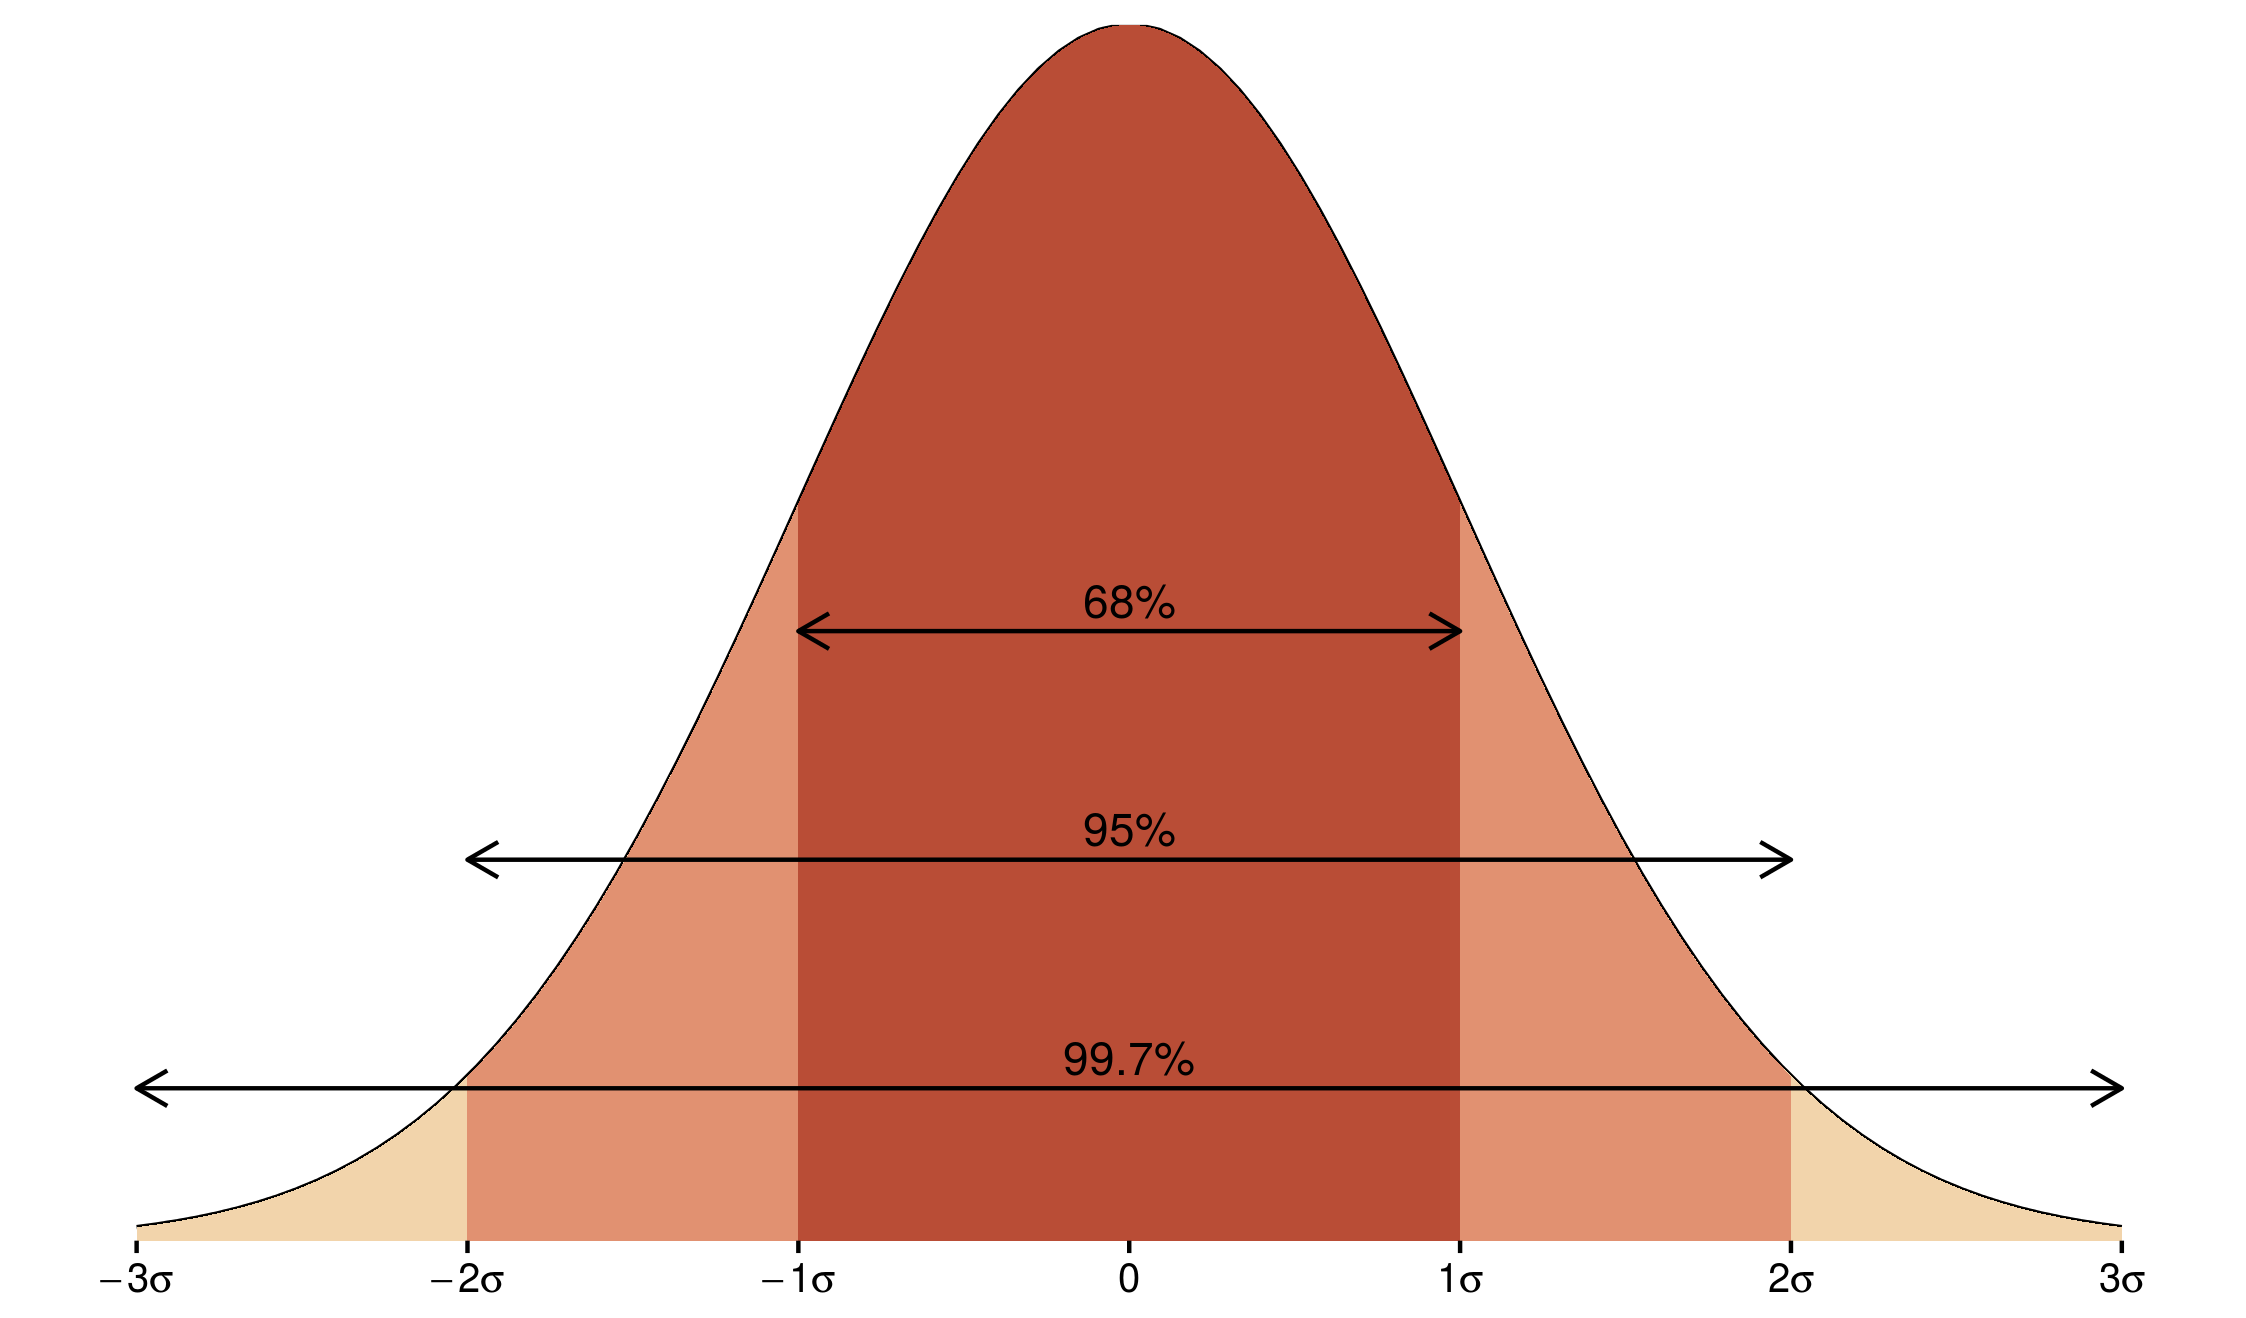
\includegraphics[width=1\linewidth]{figs/normal_distribution} 

}

\caption{Rozrzut wartości w rozkładzie normalnym w zależności od odchylenia standardowego.}\label{fig:03-eksp-analiza-danych-7}
\end{figure}

\begin{Shaded}
\begin{Highlighting}[]
\FunctionTok{sd}\NormalTok{(punkty}\SpecialCharTok{$}\NormalTok{temp, }\AttributeTok{na.rm =} \ConstantTok{TRUE}\NormalTok{)}
\end{Highlighting}
\end{Shaded}

\begin{verbatim}
## [1] 3.954922
\end{verbatim}

\subsection{Liczebność grup}\label{liczebnoux15bux107-grup}

Dla zmiennych kategoryzowanych nie powinno wyliczać się~powyższych statystyk.
Możliwe jest natomiast określenie liczebności grup używając funkcji \texttt{table()}.

\begin{Shaded}
\begin{Highlighting}[]
\FunctionTok{table}\NormalTok{(punkty}\SpecialCharTok{$}\NormalTok{clc)}
\end{Highlighting}
\end{Shaded}

\begin{verbatim}
## 
##   1   2   4 
## 165  57  20
\end{verbatim}

\section{Wykresy}\label{wykresy}

\subsection{Histogram}\label{histogram}

Histogram należy do typów wykresów najczęściej używanych w eksploracyjnej analizie danych (rycina \ref{fig:03-eksp-analiza-danych-9}).

\begin{Shaded}
\begin{Highlighting}[]
\FunctionTok{ggplot}\NormalTok{(punkty, }\FunctionTok{aes}\NormalTok{(temp)) }\SpecialCharTok{+} \FunctionTok{geom\_histogram}\NormalTok{()}
\end{Highlighting}
\end{Shaded}

\begin{figure}

{\centering 
\includegraphics[width=1\linewidth]{03-eksp_analiza_danych_files/figure-latex/03-eksp-analiza-danych-9-1} 

}

\caption{Histogram reprezentujący wartości zmiennej temp z obiektu punkty.}\label{fig:03-eksp-analiza-danych-9}
\end{figure}

Jest on graficzną reprezentacją rozkładu danych.
Wartości danych są łączone w przedziały (na osi poziomej) a na osi pionowej jest ukazana liczba punktów (obserwacji) w każdym przedziale.
Co ważne, różny dobór przedziałów może dawać inną informację - w pakiecie \textbf{ggplot2} domyślnie przedział jest ustalany poprzez podzielenie zakresu wartości przez 30.

\subsection{Estymator jądrowy gęstości}\label{estymator-jux105drowy-gux119stoux15bci}

Podobną funkcję do histogramu spełnia estymator jądrowy gęstości (ang. \emph{kernel density estimation}).
Przypomina on wygładzony wykres histogramu i również służy graficznej reprezentacji rozkładu danych (rycina \ref{fig:03-eksp-analiza-danych-10}).

\begin{Shaded}
\begin{Highlighting}[]
\FunctionTok{ggplot}\NormalTok{(punkty, }\FunctionTok{aes}\NormalTok{(temp)) }\SpecialCharTok{+} \FunctionTok{geom\_density}\NormalTok{()}
\end{Highlighting}
\end{Shaded}

\begin{figure}

{\centering 
\includegraphics[width=1\linewidth]{03-eksp_analiza_danych_files/figure-latex/03-eksp-analiza-danych-10-1} 

}

\caption{Rozkład wartości zmiennej temp z obiektu punkty.}\label{fig:03-eksp-analiza-danych-10}
\end{figure}

\subsection{Wykres kwantyl-kwantyl}\label{wykres-kwantyl-kwantyl}

Wykres kwantyl-kwantyl (ang.\emph{quantile-quantile}) ułatwia interpretację rozkładu danych (rycina \ref{fig:03-eksp-analiza-danych-11}).

\begin{Shaded}
\begin{Highlighting}[]
\FunctionTok{ggplot}\NormalTok{(punkty, }\FunctionTok{aes}\NormalTok{(}\AttributeTok{sample =}\NormalTok{ temp)) }\SpecialCharTok{+} \FunctionTok{geom\_qq}\NormalTok{()}
\end{Highlighting}
\end{Shaded}

\begin{figure}

{\centering 
\includegraphics[width=1\linewidth]{03-eksp_analiza_danych_files/figure-latex/03-eksp-analiza-danych-11-1} 

}

\caption{Wykres kwantyl-kwantyl wartości zmiennej temp z obiektu punkty.}\label{fig:03-eksp-analiza-danych-11}
\end{figure}

Na poniższej rycinie można zobaczyć przykłady najczęściej spotykanych cech rozkładu danych w wykresach kwantyl-kwantyl (rycina \ref{fig:03-eksp-analiza-danych-12}).

\begin{figure}

{\centering 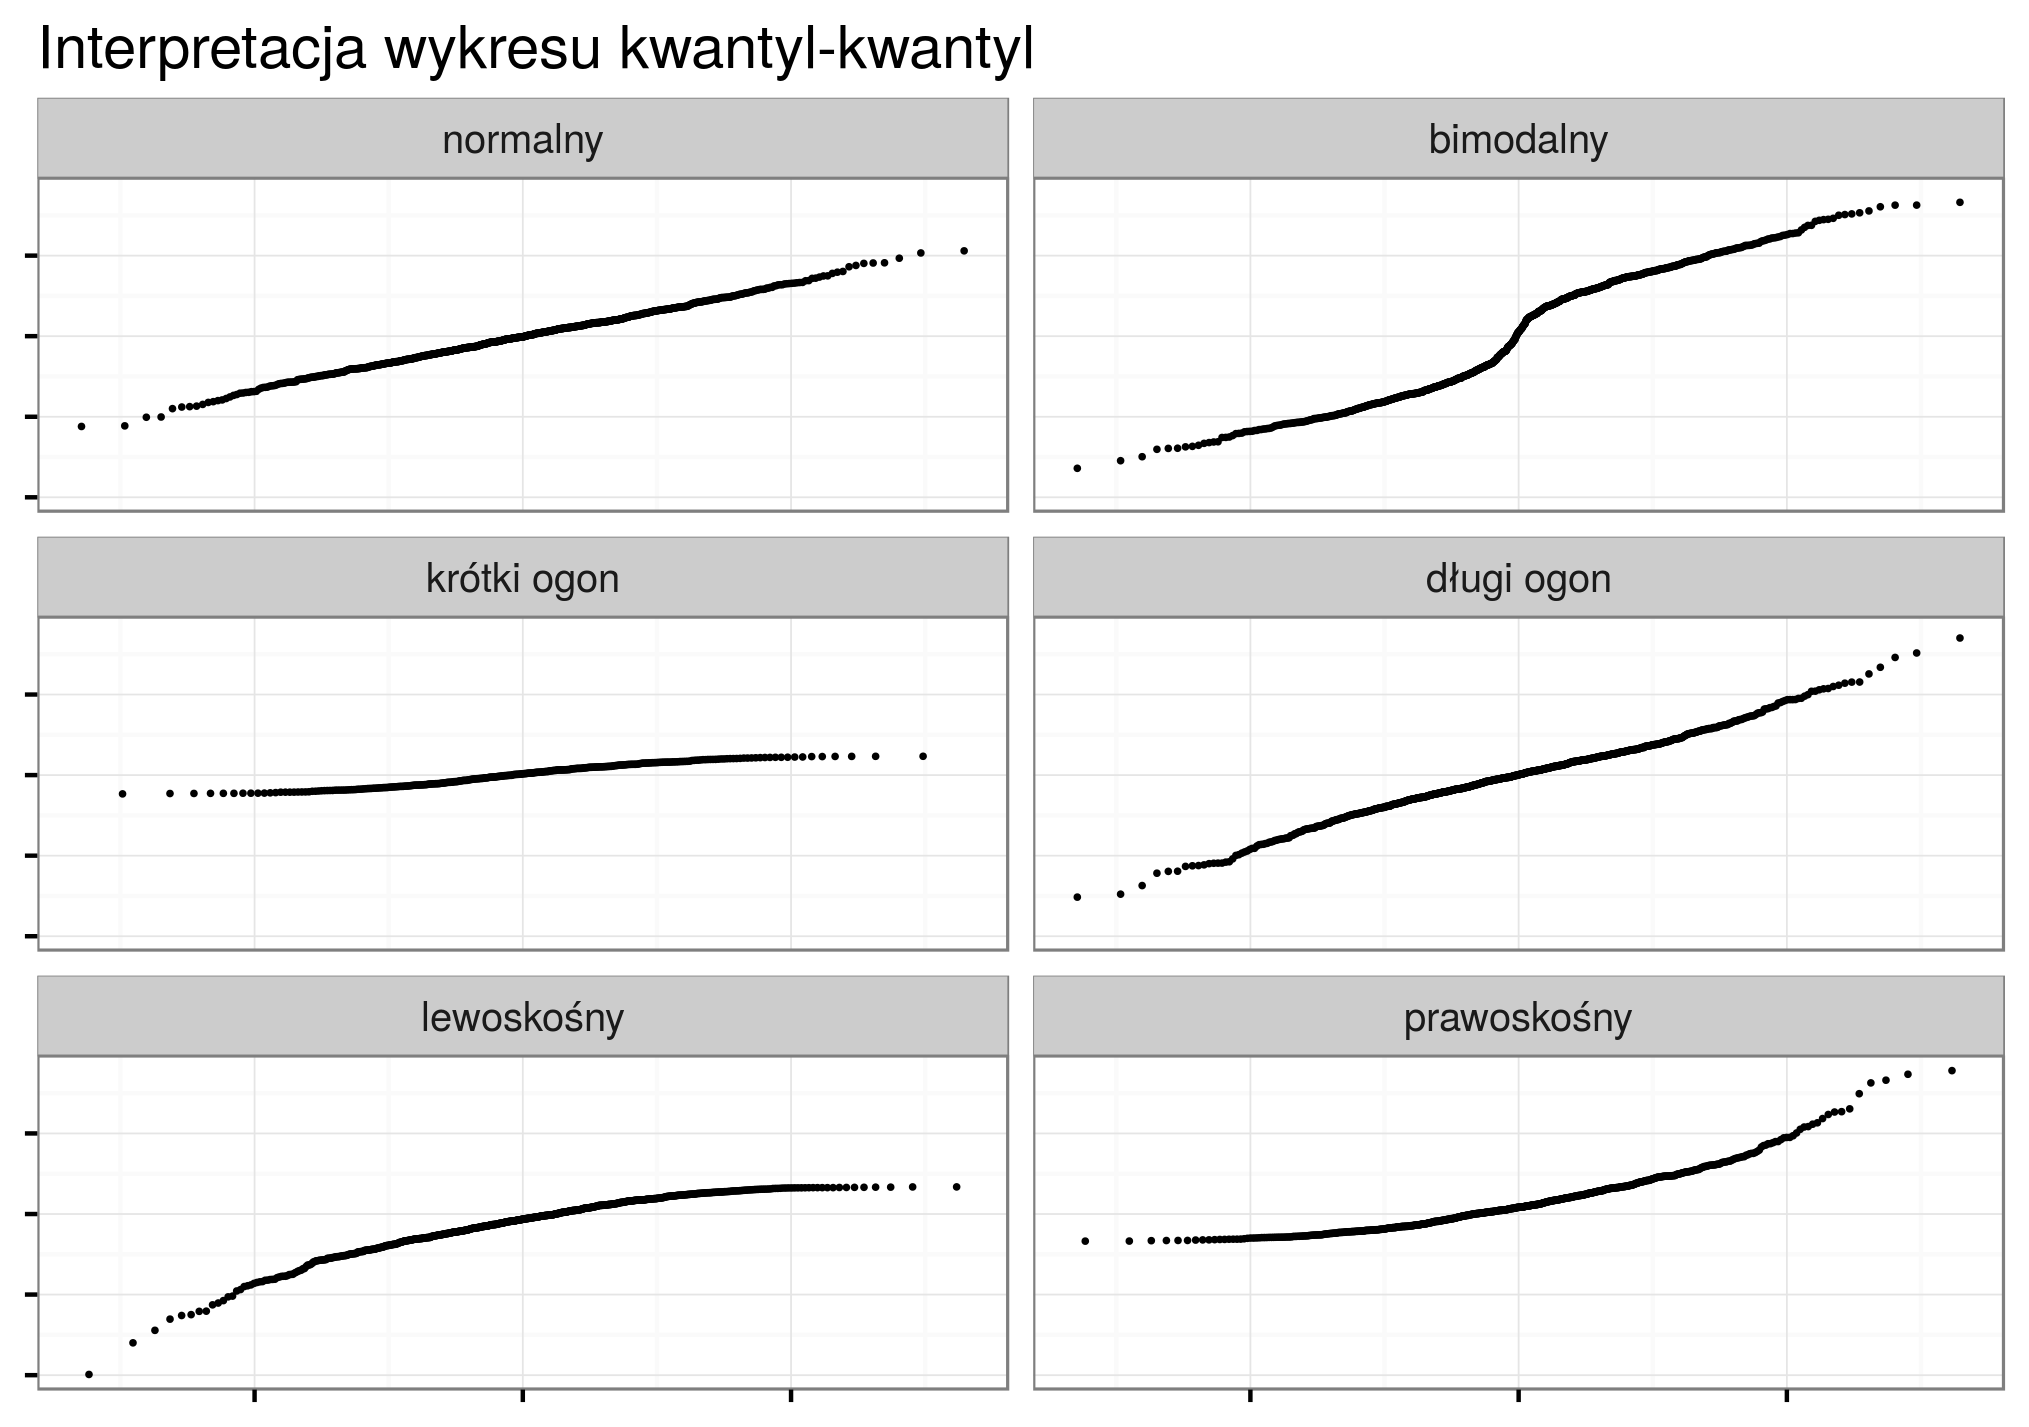
\includegraphics[width=1\linewidth]{figs/qq_plot_explained} 

}

\caption{Interpretacja rozkładu danych w zależności od wyglądu wykresu kwantyl-kwantyl.}\label{fig:03-eksp-analiza-danych-12}
\end{figure}

\subsection{Dystrybuanta (CDF)}\label{dystrybuanta-cdf}

Dystrybuanta (ang. \emph{cumulative distribution function} - CDF) wyświetla prawdopodobieństwo, że wartość zmiennej przewidywanej jest mniejsza lub równa określonej wartości (rycina \ref{fig:03-eksp-analiza-danych-13}).

\begin{Shaded}
\begin{Highlighting}[]
\FunctionTok{ggplot}\NormalTok{(punkty, }\FunctionTok{aes}\NormalTok{(temp)) }\SpecialCharTok{+} \FunctionTok{stat\_ecdf}\NormalTok{()}
\end{Highlighting}
\end{Shaded}

\begin{figure}

{\centering 
\includegraphics[width=1\linewidth]{03-eksp_analiza_danych_files/figure-latex/03-eksp-analiza-danych-13-1} 

}

\caption{Dystrybuanta zmiennej temp z obiektu punkty.}\label{fig:03-eksp-analiza-danych-13}
\end{figure}

\subsection{Wykres słupkowy}\label{wykres-sux142upkowy}

Wykres słupkowy (ang. \emph{bar plot}) przedstawia liczebność kolejnych grup (rycina \ref{fig:03-eksp-analiza-danych-13b}).

\begin{Shaded}
\begin{Highlighting}[]
\FunctionTok{ggplot}\NormalTok{(punkty, }\FunctionTok{aes}\NormalTok{(clc)) }\SpecialCharTok{+} \FunctionTok{geom\_bar}\NormalTok{()}
\end{Highlighting}
\end{Shaded}

\begin{figure}

{\centering 
\includegraphics[width=1\linewidth]{03-eksp_analiza_danych_files/figure-latex/03-eksp-analiza-danych-13b-1} 

}

\caption{Wykres słupkowy zmiennej clc z obiektu punkty.}\label{fig:03-eksp-analiza-danych-13b}
\end{figure}

\section{Porównanie zmiennych}\label{poruxf3wnanie-zmiennych}

Wybór odpowiedniej metody porównania zmiennych zależy od szeregu cech, między innymi liczby zmiennych, ich typu, rozkładu wartości, etc.

\subsection{Kowariancja}\label{kowariancja}

Kowariancja jest nieunormowaną miarą zależności liniowej pomiędzy dwiema zmiennymi.
Kowariancja dwóch zmiennych \(x\) i \(y\) pokazuje jak dwie zmienne są ze sobą liniowo powiązane.
Dodatnia kowariancja wskazuje na pozytywną relację liniową pomiędzy zmiennymi, podczas gdy ujemna kowariancja świadczy o odwrotnej sytuacji.
Jeżeli zmienne nie są ze sobą liniowo powiązane, wartość kowariancji jest bliska zeru; inaczej mówiąc, kowariancja stanowi miarę wspólnej zmienności dwóch zmiennych.
Wielkość samej kowariancji uzależniona jest od przyjętej skali zmiennej (jednostki).
Inne wyniki uzyskamy (przy tej samej zależności pomiędzy parą zmiennych), gdy będziemy analizować wyniki np. wysokości terenu w metrach i temperatury w stopniach Celsjusza a inne dla wysokości terenu w metrach i temperatury w stopniach Fahrenheita.
Do wyliczania kowariancji w R służy funkcja \texttt{cov()}.

\subsection{Współczynnik korelacji}\label{wspuxf3ux142czynnik-korelacji}

Współczynnik korelacji to unormowana miara zależności pomiędzy dwiema zmiennymi, przyjmująca wartości od -1 do 1.
Ten współczynnik jest uzyskiwany poprzez podzielenie wartości kowariancji przez odchylenie standardowe wyników.
Z racji unormowania nie jest ona uzależniona od jednostki.
Korelację można wyliczyć dzięki funkcji \texttt{cor()} (rycina \ref{fig:03-eksp-analiza-danych-15a}).
Działa ona zarówno w przypadku dwóch zmiennych numerycznych, jak i całego obiektu zawierającego zmienne numeryczne.
Za pomocą argumentu \texttt{method} można również wybrać jedną z trzech dostępnych miar korelacji: \texttt{"pearson"} przeznaczoną dla zmiennych o rozkładzie normalnym oraz \texttt{"spearman"} i \texttt{"kendall"} używaną dla zmiennych o rozkładzie różnym od normalnego.

\begin{Shaded}
\begin{Highlighting}[]
\FunctionTok{cor}\NormalTok{(punkty}\SpecialCharTok{$}\NormalTok{temp, punkty}\SpecialCharTok{$}\NormalTok{ndvi, }\AttributeTok{method =} \StringTok{"spearman"}\NormalTok{)}
\end{Highlighting}
\end{Shaded}

\begin{verbatim}
## [1] 0.04499375
\end{verbatim}

\begin{Shaded}
\begin{Highlighting}[]
\FunctionTok{ggplot}\NormalTok{(punkty, }\FunctionTok{aes}\NormalTok{(temp, ndvi)) }\SpecialCharTok{+} \FunctionTok{geom\_point}\NormalTok{()}
\end{Highlighting}
\end{Shaded}

\begin{figure}

{\centering 
\includegraphics[width=1\linewidth]{03-eksp_analiza_danych_files/figure-latex/03-eksp-analiza-danych-15a-1} 

}

\caption{Wykres rozrzutu reprezentujący relację pomiędzy zmienną temp i ndvi z obiektu punkty.}\label{fig:03-eksp-analiza-danych-15a}
\end{figure}

Dodatkowo funkcja \texttt{cor.test()} służy do testowania istotności korelacji.

\begin{Shaded}
\begin{Highlighting}[]
\FunctionTok{cor.test}\NormalTok{(punkty}\SpecialCharTok{$}\NormalTok{temp, punkty}\SpecialCharTok{$}\NormalTok{ndvi, }\AttributeTok{method =} \StringTok{"spearman"}\NormalTok{)}
\end{Highlighting}
\end{Shaded}

\begin{verbatim}
## 
##  Spearman's rank correlation rho
## 
## data:  punkty$temp and punkty$ndvi
## S = 2255764, p-value = 0.486
## alternative hypothesis: true rho is not equal to 0
## sample estimates:
##        rho 
## 0.04499375
\end{verbatim}

\subsection{Wykres pudełkowy}\label{wykres-pudeux142kowy}

Wykres pudełkowy obrazuje pięć podstawowych statystyk opisowych oraz wartości odstające (rycina \ref{fig:03-eksp-analiza-danych-17}).
Pudełko to zakres międzykwartylowy (IQR), a linie oznaczają najbardziej ekstremalne wartości, ale nie odstające.
Górna z nich to 1,5*IQR ponad krawędź pudełka, dolna to 1,5*IQR poniżej wartości dolnej krawędzi pudełka.
Linia środkowa to mediana.

\begin{Shaded}
\begin{Highlighting}[]
\NormalTok{punkty}\SpecialCharTok{$}\NormalTok{clc }\OtherTok{=} \FunctionTok{as.factor}\NormalTok{(punkty}\SpecialCharTok{$}\NormalTok{clc)}
\FunctionTok{ggplot}\NormalTok{(punkty, }\FunctionTok{aes}\NormalTok{(}\AttributeTok{x =}\NormalTok{ clc, }\AttributeTok{y =}\NormalTok{ temp)) }\SpecialCharTok{+} \FunctionTok{geom\_boxplot}\NormalTok{()}
\end{Highlighting}
\end{Shaded}

\begin{figure}

{\centering 
\includegraphics[width=1\linewidth]{03-eksp_analiza_danych_files/figure-latex/03-eksp-analiza-danych-17-1} 

}

\caption{Wykres pudełkowy pokazujący relację pomiędzy zmienną clc i temp z obiektu punkty.}\label{fig:03-eksp-analiza-danych-17}
\end{figure}

\subsection{Testowanie istotności różnić średniej pomiędzy grupami}\label{testowanie-istotnoux15bci-ruxf3ux17cniux107-ux15bredniej-pomiux119dzy-grupami}

Analiza wariancji (ang. \emph{Analysis of Variance} - ANOVA) służy do testowania istotności różnic między średnimi w wielu grupach.
Metoda ta służy do oceny czy średnie wartości cechy \(Y\) różnią się istotnie pomiędzy grupami wyznaczonymi przez zmienną \(X\).
ANOVA nie pozwala natomiast na stwierdzenie między którymi grupami występują różnice.
Aby to stwierdzić konieczne jest wykonanie porównań wielokrotnych (\emph{post-hoc}).
ANOVĘ można wykonać za pomocą funkcji \texttt{aov()} definiując zmienną zależną oraz zmienną grupującą oraz zbiór danych.

\begin{Shaded}
\begin{Highlighting}[]
\NormalTok{punkty}\SpecialCharTok{$}\NormalTok{clc }\OtherTok{=} \FunctionTok{as.factor}\NormalTok{(punkty}\SpecialCharTok{$}\NormalTok{clc)}
\NormalTok{aov\_test }\OtherTok{=} \FunctionTok{aov}\NormalTok{(temp }\SpecialCharTok{\textasciitilde{}}\NormalTok{ clc, }\AttributeTok{data =}\NormalTok{ punkty)}
\FunctionTok{summary}\NormalTok{(aov\_test)}
\end{Highlighting}
\end{Shaded}

\begin{verbatim}
##              Df Sum Sq Mean Sq F value              Pr(>F)    
## clc           2   1272   636.0   60.86 <0.0000000000000002 ***
## Residuals   239   2498    10.4                                
## ---
## Signif. codes:  0 '***' 0.001 '**' 0.01 '*' 0.05 '.' 0.1 ' ' 1
\end{verbatim}

Do wykonania porównań wielokrotnych służy funkcja \texttt{TukeyHSD()}.
Dodatkowo wyniki można wizualizować za pomocą funkcji \texttt{plot()} (rycina \ref{fig:03-eksp-analiza-danych-20}).

\begin{Shaded}
\begin{Highlighting}[]
\NormalTok{tukey }\OtherTok{=} \FunctionTok{TukeyHSD}\NormalTok{(aov\_test, }\StringTok{"clc"}\NormalTok{)}
\FunctionTok{plot}\NormalTok{(tukey, }\AttributeTok{las =} \DecValTok{1}\NormalTok{)}
\end{Highlighting}
\end{Shaded}

\begin{figure}

{\centering 
\includegraphics[width=1\linewidth]{03-eksp_analiza_danych_files/figure-latex/03-eksp-analiza-danych-20-1} 

}

\caption{Graficzna reprezentacja wyniku porównań wielokrotnych.}\label{fig:03-eksp-analiza-danych-20}
\end{figure}

\section{Transformacje danych}\label{trans-danych}

\subsection{Cel transformacji danych}\label{cel-transformacji-danych}

Transformacja danych może mieć na celu ułatwienie porównywania różnych zmiennych, zniwelowanie skośności rozkładu lub też zmniejszenie wpływu danych odstających.
W efekcie transformacja danych ułatwia przeprowadzenie analiz (geo-)statystycznych i polepsza wyniki prognoz z modeli.
Przykładowo, możliwe jest stworzenie modelu i estymacji używając logarytmu badanej zmiennej, a następnie przywrócenie oryginalnej jednostki danych.

Redukcja skośności może być przeprowadzona z na wiele sposób.
Jednym z najpopularniejszych jest użycie transformacji logarytmicznej.

\subsection{Testowanie normalności rozkładu}\label{testowanie-normalnoux15bci-rozkux142adu}

Test Shapiro-Wilka pozwala na sprawdzenie normalności rozkładu wybranej zmiennej.
Hipoteza zerowa tego testu mówi, że rozkład badanej zmiennej jest zbliżony do normalnego, natomiast hipoteza alternatywna stwierdza, że ten rozkład jest różny od normalnego.

\begin{Shaded}
\begin{Highlighting}[]
\FunctionTok{shapiro.test}\NormalTok{(punkty}\SpecialCharTok{$}\NormalTok{temp)}
\end{Highlighting}
\end{Shaded}

\begin{verbatim}
## 
##  Shapiro-Wilk normality test
## 
## data:  punkty$temp
## W = 0.96904, p-value = 0.00004054
\end{verbatim}

W powyższym przypadku, \emph{p-value} jest niskie, sugerując, że musimy odrzucić hipotezę zerową i przyjąć alternatywną: rozkład zmiennej \texttt{temp} jest różny od normalnego.

\subsection{Logarytmizacja}\label{logarytmizacja}

Jedną grupą technik służących redukcji skośności jest logarytmizacja.
Logarytmizacja w R może odbyć się za pomocą funkcji \texttt{log()} (rycina \ref{fig:03-eksp-analiza-danych-28}).

\begin{Shaded}
\begin{Highlighting}[]
\NormalTok{punkty}\SpecialCharTok{$}\NormalTok{log\_tpz }\OtherTok{=} \FunctionTok{log}\NormalTok{(punkty}\SpecialCharTok{$}\NormalTok{temp)}
\end{Highlighting}
\end{Shaded}

\begin{figure}

{\centering 
\includegraphics[width=1\linewidth]{03-eksp_analiza_danych_files/figure-latex/03-eksp-analiza-danych-28-1} 

}

\caption{Porównania wartości zmiennej temp przed i po transformacji logaritmicznej.}\label{fig:03-eksp-analiza-danych-28}
\end{figure}

\subsection{Transformacja odwrotna}\label{transformacja-odwrotna}

Przywrócenie wartości do oryginalnej jednostki, np. po estymacji, wymaga zastosowania odpowiedniej metody transformacji wstecznej \href{https://link.springer.com/article/10.1007/s10596-007-9046-x}{(Yamamoto, 2007)}.

\[y = k_0 \cdot exp[ln(\hat{y}_{OK})+\frac{\sigma^2_{OK}}{2}]\]

, gdzie:

\begin{itemize}
\tightlist
\item
  \(k_0\) - współczynnik korekcyjny (iloraz średniej oryginalnej i średniej po transformacji wstecznej)
\item
  \(exp\) - funkcja wykładnicza
\item
  \(ln\) - funkcja logarytmiczna
\item
  \(\hat{y}_{OK}\) - estymacja krigingu zwykłego
\item
  \(\sigma^2_{OK}\) - wariacja krigingu zwykłego
\end{itemize}

Zobaczmy to na uproszczonym przykładzie.
Poniższy blok kodu tworzy model semiwariogramy, a następnie estymację dla badanego obszaru.
Wyjaśnienie działania poniższych linii kodu można znaleźć w rozdziałach \ref{geostatystyka-prolog}, \ref{modelowanie-matematycznie-autokorelacji-przestrzennej} i \ref{estymacje-jednozmienne}.

\begin{Shaded}
\begin{Highlighting}[]
\FunctionTok{library}\NormalTok{(gstat)}
\FunctionTok{data}\NormalTok{(siatka)}
\NormalTok{vario }\OtherTok{=} \FunctionTok{variogram}\NormalTok{(log\_tpz }\SpecialCharTok{\textasciitilde{}} \DecValTok{1}\NormalTok{, }\AttributeTok{locations =}\NormalTok{ punkty)}
\NormalTok{model }\OtherTok{=} \FunctionTok{fit.variogram}\NormalTok{(vario, }\FunctionTok{vgm}\NormalTok{(}\AttributeTok{model =} \StringTok{"Sph"}\NormalTok{, }\AttributeTok{nugget =} \FloatTok{0.5}\NormalTok{))}
\NormalTok{ok }\OtherTok{=} \FunctionTok{krige}\NormalTok{(log\_tpz }\SpecialCharTok{\textasciitilde{}} \DecValTok{1}\NormalTok{,}
            \AttributeTok{locations =}\NormalTok{ punkty,}
            \AttributeTok{newdata =}\NormalTok{ siatka, }
            \AttributeTok{model =}\NormalTok{ model)}
\end{Highlighting}
\end{Shaded}

\begin{verbatim}
## [using ordinary kriging]
\end{verbatim}

Wynik, obiekt \texttt{ok} jest rastrem zawierającym dwie warstwy: \texttt{var1.pred} i \texttt{var1.var}.
Pierwsza z nich, \texttt{var1.pred}, zawiera estymowane wartości dla każdego oczka siatki, jednak ich jednostkami jest logarytm oryginalnej jednostki (\(ln(\hat{y}_{OK})\)).
Druga warstwa, \texttt{var1.var}, opisuje wariancję (niepewność) pomiaru w każdym oczku siatki (\(\sigma^2_{OK}\)).

Wartości z obu tych warstw możemy podstawić do powyższego wzoru.

\begin{Shaded}
\begin{Highlighting}[]
\NormalTok{bt }\OtherTok{=} \FunctionTok{exp}\NormalTok{(ok}\SpecialCharTok{$}\NormalTok{var1.pred }\SpecialCharTok{+}\NormalTok{ (ok}\SpecialCharTok{$}\NormalTok{var1.var }\SpecialCharTok{/} \DecValTok{2}\NormalTok{))}
\end{Highlighting}
\end{Shaded}

W kolejnym kroku musimy wyliczyć, \(k_0\), współczynnik korekcyjny.
Jest to iloraz średniej oryginalnej i średniej po transformacji wstecznej.

\begin{Shaded}
\begin{Highlighting}[]
\NormalTok{mu\_bt }\OtherTok{=} \FunctionTok{mean}\NormalTok{(bt, }\AttributeTok{na.rm =} \ConstantTok{TRUE}\NormalTok{)}
\NormalTok{mu\_original }\OtherTok{=} \FunctionTok{mean}\NormalTok{(punkty}\SpecialCharTok{$}\NormalTok{temp, }\AttributeTok{na.rm =} \ConstantTok{TRUE}\NormalTok{)}
\NormalTok{k0 }\OtherTok{=}\NormalTok{ mu\_original }\SpecialCharTok{/}\NormalTok{ mu\_bt}
\end{Highlighting}
\end{Shaded}

Do otrzymania wynikowych wartości w oryginalnej jednostce musimy teraz pomnożyć wartości po transformacji wstecznej ze współczynnikiem korekcyjnym (rycina \ref{fig:03-eksp-analiza-danych-28b}).

\begin{Shaded}
\begin{Highlighting}[]
\NormalTok{btt }\OtherTok{=}\NormalTok{ bt }\SpecialCharTok{*}\NormalTok{ k0}
\end{Highlighting}
\end{Shaded}

\begin{figure}

{\centering 
\includegraphics[width=1\linewidth]{03-eksp_analiza_danych_files/figure-latex/03-eksp-analiza-danych-28b-1} 

}

\caption{Porównania wartości zmiennej temp przed, po transformacji logaritmicznej, oraz po transformacji odwrotnej.}\label{fig:03-eksp-analiza-danych-28b}
\end{figure}

Finalnie możliwe jest też wpisanie wartości po transformacji odwrotnej do siatki.

\begin{Shaded}
\begin{Highlighting}[]
\NormalTok{ok}\SpecialCharTok{$}\NormalTok{var1.pred2 }\OtherTok{=}\NormalTok{ btt   }
\end{Highlighting}
\end{Shaded}

Aby uprościć sobie transformacje odwrotne w przyszłości, możemy powyższy kod przepisać do postaci funkcji \texttt{rev\_trans()}:

\begin{Shaded}
\begin{Highlighting}[]
\NormalTok{rev\_trans }\OtherTok{=} \ControlFlowTok{function}\NormalTok{(pred, var, obs)\{}
\NormalTok{        bt }\OtherTok{=} \FunctionTok{exp}\NormalTok{(pred }\SpecialCharTok{+}\NormalTok{ (var }\SpecialCharTok{/} \DecValTok{2}\NormalTok{))}
\NormalTok{        mu\_bt }\OtherTok{=} \FunctionTok{mean}\NormalTok{(bt, }\AttributeTok{na.rm =} \ConstantTok{TRUE}\NormalTok{)}
\NormalTok{        mu\_original }\OtherTok{=} \FunctionTok{mean}\NormalTok{(obs, }\AttributeTok{na.rm =} \ConstantTok{TRUE}\NormalTok{)}
\NormalTok{        k0 }\OtherTok{=}\NormalTok{ mu\_original }\SpecialCharTok{/}\NormalTok{ mu\_bt}
\NormalTok{        btt }\OtherTok{=}\NormalTok{ bt }\SpecialCharTok{*}\NormalTok{ k0}
        \FunctionTok{return}\NormalTok{(btt)}
\NormalTok{\}}
\end{Highlighting}
\end{Shaded}

Funkcja \texttt{rev\_trans()} przyjmuje trzy argumenty:

\begin{itemize}
\tightlist
\item
  \texttt{pred} - estymowane wartości, których jednostką jest logarytm oryginalnej jednostki
\item
  \texttt{var} - wariancja kolejnych estymacji
\item
  \texttt{obs} - wartości pomiarów w punktach w oryginalnej jednostce
\end{itemize}

Dla ułatwienia funkcja \texttt{rev\_trans()} znajduje się też w pakiecie \textbf{geostatbook}.

\section{Zadania}\label{z3}

Przyjrzyj się~danym z obiektu \texttt{punkty\_pref}.
Możesz go wczytać używając poniższego kodu:

\begin{Shaded}
\begin{Highlighting}[]
\FunctionTok{data}\NormalTok{(punkty\_pref)}
\end{Highlighting}
\end{Shaded}

\begin{enumerate}
\def\labelenumi{\arabic{enumi}.}
\tightlist
\item
  Ile obserwacji i zmiennych jest zawartych w tym obiekcie?
  Jaka jest jego klasa?
\item
  Określ i opisz podstawowe statystyki opisowe zmiennej \texttt{ndvi}.
\item
  Stwórz histogram obrazujący rozkład tej zmiennej.
  Czym charakteryzuje się ten rozkład?
\item
  Jakie jest prawdopodobieństwo przekroczenia wartości \texttt{ndvi} 0.4 w tym zbiorze danych?
\item
  Określ korelację pomiędzy zmienną \texttt{ndvi} a \texttt{savi}.
  Czy jest ona istotna statystycznie?
\item
  Zbuduj wykres pokazujący zmienność \texttt{ndvi} w zależności od klasy pokrycia terenu.
  Czy istnieje istotna statystycznie różnica w wartościach \texttt{ndvi} względem klas pokrycia terenu?
\item
  Wypróbuj logarytmizację danych na zmiennej \texttt{ndvi}.
  Czy poprawiła ona właściwości rozkładu tej zmiennej?
\end{enumerate}

\chapter{Eksploracyjna analiza danych przestrzennych}\label{eksploracyjna-analiza-danych-przestrzennych}

Odtworzenie obliczeń z tego rozdziału wymaga załączenia poniższych pakietów oraz wczytania poniższych danych:

\begin{Shaded}
\begin{Highlighting}[]
\FunctionTok{library}\NormalTok{(sf)}
\FunctionTok{library}\NormalTok{(stars)}
\FunctionTok{library}\NormalTok{(tmap)}
\FunctionTok{library}\NormalTok{(geostatbook)}
\FunctionTok{data}\NormalTok{(punkty)}
\FunctionTok{data}\NormalTok{(granica)}
\end{Highlighting}
\end{Shaded}

\section{Aspekt przestrzenny}\label{aspekt-przestrzenny}

\subsection{Podstawowe terminy}\label{podstawowe-terminy}

\begin{itemize}
\tightlist
\item
  Populacja - cały obszar, dla którego chcemy określić wybrane właściwości, np. temperatura powietrza.
\item
  Próba - zbiór obserwacji, dla których mamy informacje, np. pomiary ze stacji meteorologicznych.
  Inaczej, próba to podzbiór populacji.
\end{itemize}

Zazwyczaj niemożliwe (lub bardzo kosztowne) jest zdobycie informacji o całej populacji.
Z tego powodu bardzo cenne jest odpowiednie wykorzystanie informacji z próby, a następnie wnioskowanie na jej podstawie o populacji.

\subsection{Mapy punktowe}\label{mapy-punktowe}

Eksploracyjna analiza danych przestrzennych w przypadku danych punktowych ma na celu:

\begin{itemize}
\tightlist
\item
  Sprawdzenie poprawności współrzędnych (sekcja \ref{popr-wsp}).
\item
  Sprawdzenie poprawności danych, w tym między innymi określenie danych odstających lokalnie (sekcja \ref{dane-odst}).
\item
  Wgląd w typ próbkowania danych (sekcja \ref{probkowanie}).
\item
  Rozgrupowanie danych przy próbkowaniu preferencyjnym (sekcja \ref{rozgrupowanie}).
\item
  Ogólny pogląd na zmienność przestrzenną, wykorzystanie prostej automatycznej procedury interpolacji (rozdział \ref{metody-interpolacji}).
\end{itemize}

\section{Sprawdzenie poprawności współrzędnych}\label{popr-wsp}

Wstępne sprawdzenie poprawności współrzędnych można wykonać poprzez wizualizację danych przestrzennych za pomocą funkcji \texttt{plot()} (rycina \ref{fig:04-eksp-przestrzenna-3}).

\begin{Shaded}
\begin{Highlighting}[]
\FunctionTok{tm\_shape}\NormalTok{(granica) }\SpecialCharTok{+}
        \FunctionTok{tm\_polygons}\NormalTok{() }\SpecialCharTok{+}
        \FunctionTok{tm\_shape}\NormalTok{(punkty) }\SpecialCharTok{+}
        \FunctionTok{tm\_symbols}\NormalTok{() }\SpecialCharTok{+}
        \FunctionTok{tm\_grid}\NormalTok{()}
\end{Highlighting}
\end{Shaded}

\begin{figure}

{\centering 
\includegraphics[width=1\linewidth]{04-eksp_przestrzenna_files/figure-latex/04-eksp-przestrzenna-3-1} 

}

\caption{Lokalizacja punktów pomiarowych na tle granicy obszaru badań.}\label{fig:04-eksp-przestrzenna-3}
\end{figure}

\section{Dane lokalnie odstające}\label{dane-odst}

Dane lokalnie odstające oznaczają nietypowe przestrzennie wartości danej cechy; nie zawsze możliwe jest ich określenie używając statystyk opisowych czy histogramów.
Daną lokalnie odstającą może być przykładowo niska wartość otoczona wysokimi wartościami lub też wysoka wartość otoczona niskimi wartościami.
Może to oznaczać zarówno błąd w danych albo wpływ innego czynnika na analizowaną cechę.
Przyjrzenie się wartościom analizowanej cechy można wykonać z użyciem funkcji \texttt{plot()}.
Na poniższym przykładzie wyświetlona jest zmienna \texttt{temp} oznaczająca średnią temperaturę dobową (rycina \ref{fig:04-eksp-przestrzenna-8}).

\begin{Shaded}
\begin{Highlighting}[]
\FunctionTok{tm\_shape}\NormalTok{(granica) }\SpecialCharTok{+}
        \FunctionTok{tm\_polygons}\NormalTok{() }\SpecialCharTok{+}
        \FunctionTok{tm\_shape}\NormalTok{(punkty) }\SpecialCharTok{+}
        \FunctionTok{tm\_symbols}\NormalTok{(}\AttributeTok{col =} \StringTok{"temp"}\NormalTok{, }\AttributeTok{n =} \DecValTok{10}\NormalTok{) }\SpecialCharTok{+}
        \FunctionTok{tm\_layout}\NormalTok{(}\AttributeTok{legend.outside =} \ConstantTok{TRUE}\NormalTok{)}
\end{Highlighting}
\end{Shaded}

\begin{figure}

{\centering 
\includegraphics[width=1\linewidth]{04-eksp_przestrzenna_files/figure-latex/04-eksp-przestrzenna-8-1} 

}

\caption{Wizualizacja zmiennej temp pozwalająca na wyszukanie wartości lokalnie odstających.}\label{fig:04-eksp-przestrzenna-8}
\end{figure}

Dodatkowo można wykorzystać tryb \texttt{view} w pakiecie \textbf{tmap} do interaktywnego określania wartości oraz numeru punktu (numer wiersza w tabeli atrybutów).

\begin{Shaded}
\begin{Highlighting}[]
\FunctionTok{tmap\_mode}\NormalTok{(}\StringTok{"view"}\NormalTok{)}
\FunctionTok{tm\_shape}\NormalTok{(punkty) }\SpecialCharTok{+}
        \FunctionTok{tm\_symbols}\NormalTok{(}\AttributeTok{col =} \StringTok{"temp"}\NormalTok{, }\AttributeTok{n =} \DecValTok{10}\NormalTok{)}
\end{Highlighting}
\end{Shaded}

Aby powrócić do trybu statycznego, trzeba użyć funkcji \texttt{tmap\_mode("plot")}.

\begin{Shaded}
\begin{Highlighting}[]
\FunctionTok{tmap\_mode}\NormalTok{(}\StringTok{"plot"}\NormalTok{)}
\end{Highlighting}
\end{Shaded}

\section{Próbkowanie}\label{probkowanie}

\subsection{Podstawowe typy próbowania}\label{podstawowe-typy-pruxf3bowania}

Istnieje cały szereg typów próbkowania danych przestrzennych.
Funkcja \texttt{st\_sample()} z pakietu \textbf{sf} pozwala na stworzenie kilku typów próbkowania (argument \texttt{type}), między innymi:

\begin{itemize}
\tightlist
\item
  Regularny (ang.\emph{regular})
\item
  Losowy (ang.\emph{random})
\item
  Losowy stratyfikowany (ang.\emph{stratified})
\item
  Preferencyjny (ang.\emph{clustered})
\end{itemize}

\subsection{Regularny typ próbowania}\label{regularny-typ-pruxf3bowania}

W regularnym typie próbkowania, kolejne punkty rozłożone są równomiernie na badanym obszarze (rycina \ref{fig:04-eksp-przestrzenna-4}).

\begin{figure}

{\centering 
\includegraphics[width=1\linewidth]{04-eksp_przestrzenna_files/figure-latex/04-eksp-przestrzenna-4-1} 

}

\caption{Przykład próbkowania regularnego.}\label{fig:04-eksp-przestrzenna-4}
\end{figure}

\subsection{Losowy typ próbowania}\label{losowy-typ-pruxf3bowania}

W losowym typie próbkowania każda lokalizacja ma takie samo prawdopodobieństwo wystąpienia.
Dodatkowo, każdy punkt jest losowany niezależnie od pozostałych (rycina \ref{fig:04-eksp-przestrzenna-5}).

\begin{figure}

{\centering 
\includegraphics[width=1\linewidth]{04-eksp_przestrzenna_files/figure-latex/04-eksp-przestrzenna-5-1} 

}

\caption{Przykład próbkowania losowego.}\label{fig:04-eksp-przestrzenna-5}
\end{figure}

\subsection{Losowy stratyfikowany typ próbowania}\label{losowy-stratyfikowany-typ-pruxf3bowania}

Losowy stratyfikowany typ próbkowania polega na podzieleniu analizowanego obszaru na regularne komórki, a następnie dla każdej komórki losowana jest lokalizacja punktu (rycina \ref{fig:04-eksp-przestrzenna-6b}).

\begin{figure}

{\centering 
\includegraphics[width=1\linewidth]{04-eksp_przestrzenna_files/figure-latex/04-eksp-przestrzenna-6b-1} 

}

\caption{Przykład próbkowania losowego stratyfikowanego.}\label{fig:04-eksp-przestrzenna-6b}
\end{figure}

\subsection{Preferencyjny typ próbowania}\label{preferencyjny-typ-pruxf3bowania}

W preferencyjnym typie próbkowania istnieją obszary, które z jakieś powodu (np. specyficzne wartości analizowanej cechy) są znacznie częściej opróbowane niż inne (rycina \ref{fig:04-eksp-przestrzenna-7b}).

\begin{figure}

{\centering 
\includegraphics[width=1\linewidth]{04-eksp_przestrzenna_files/figure-latex/04-eksp-przestrzenna-7b-1} 

}

\caption{Przykład próbkowania preferencyjnego.}\label{fig:04-eksp-przestrzenna-7b}
\end{figure}

\section{Rozgrupowanie danych}\label{rozgrupowanie}

Typ próbkowania może wpływać na wartości statystyk opisowych.
W odpowiedzi na to istnieje szereg metod rozgrupowywania danych, wśród których można wymienić, między innymi, rozgrupowywanie poligonalne oraz rozgrupowywanie komórkowe.
Celem tych metod jest nadanie wag obserwacjom w celu zapewnienia reprezentatywności przestrzennej danych.

Na potrzeby przykładów związanych z rozgrupowaniem danych w pakiecie \textbf{geostatbook} znajduje się zbiór danych \texttt{punkty\_pref}.
W tym zbiorze gęściej opróbkowane są niskie wartości temperatury, co powoduje, że średnia dla całego obszaru jest znacznie niższa niż w rzeczywistości.

\begin{Shaded}
\begin{Highlighting}[]
\FunctionTok{data}\NormalTok{(punkty\_pref)}
\FunctionTok{tm\_shape}\NormalTok{(punkty\_pref) }\SpecialCharTok{+}
        \FunctionTok{tm\_symbols}\NormalTok{(}\AttributeTok{col =} \StringTok{"temp"}\NormalTok{, }\AttributeTok{n =} \DecValTok{10}\NormalTok{)}
\end{Highlighting}
\end{Shaded}

\begin{center}
\includegraphics[width=1\linewidth]{04-eksp_przestrzenna_files/figure-latex/unnamed-chunk-1-1} \end{center}

\begin{Shaded}
\begin{Highlighting}[]
\NormalTok{srednia\_arytmetyczna }\OtherTok{=} \FunctionTok{mean}\NormalTok{(punkty\_pref}\SpecialCharTok{$}\NormalTok{temp, }\AttributeTok{na.rm =} \ConstantTok{TRUE}\NormalTok{)}
\NormalTok{srednia\_arytmetyczna}
\end{Highlighting}
\end{Shaded}

\begin{verbatim}
## [1] 14.06929
\end{verbatim}

\subsection{Rozgrupowanie poligonalne}\label{rozgrupowanie-poligonalne}

\textbf{Rozgrupowanie poligonalne} polega na zastosowaniu jednej z metod triangulacji, np. poligonów Woronoja:

\begin{enumerate}
\def\labelenumi{\arabic{enumi}.}
\tightlist
\item
  Dla każdego punktu określany jest poligon
\item
  Wyliczana jest powierzchnia poligonu
\item
  Waga każdego punktu wyliczana jest poprzez podzielenie powierzchni indywidualnych przez powierzchnię całego obszaru, a następnie pomnożenie przez liczbę punktów
\end{enumerate}

\[w'_j=\frac{area_j}{\sum_{j=1}^{n}area_j} \cdot n\]
, gdzie \(area_j\) powierzchnia dla wybranej obserwacji, a \(n\) to łączna liczba obserwacji

\begin{Shaded}
\begin{Highlighting}[]
\FunctionTok{library}\NormalTok{(dismo)}
\NormalTok{punkty\_pref}\SpecialCharTok{$}\NormalTok{id }\OtherTok{=} \DecValTok{1}\SpecialCharTok{:}\FunctionTok{nrow}\NormalTok{(punkty\_pref)}
\NormalTok{v }\OtherTok{=} \FunctionTok{st\_as\_sf}\NormalTok{(}\FunctionTok{voronoi}\NormalTok{(}\FunctionTok{as}\NormalTok{(punkty\_pref, }\StringTok{"Spatial"}\NormalTok{)))}
\NormalTok{v}\SpecialCharTok{$}\NormalTok{pow }\OtherTok{=} \FunctionTok{as.numeric}\NormalTok{(}\FunctionTok{st\_area}\NormalTok{(v))}
\NormalTok{v}\SpecialCharTok{$}\NormalTok{waga\_rp }\OtherTok{=}\NormalTok{ v}\SpecialCharTok{$}\NormalTok{pow }\SpecialCharTok{/} \FunctionTok{sum}\NormalTok{(v}\SpecialCharTok{$}\NormalTok{pow) }\SpecialCharTok{*} \FunctionTok{nrow}\NormalTok{(punkty\_pref)}
\NormalTok{v\_df }\OtherTok{=} \FunctionTok{st\_drop\_geometry}\NormalTok{(v[}\FunctionTok{c}\NormalTok{(}\StringTok{"id"}\NormalTok{, }\StringTok{"waga\_rp"}\NormalTok{)])}
\NormalTok{punkty\_pref }\OtherTok{=} \FunctionTok{merge}\NormalTok{(punkty\_pref, v\_df, }\AttributeTok{by =} \StringTok{"id"}\NormalTok{)}
\end{Highlighting}
\end{Shaded}

\begin{Shaded}
\begin{Highlighting}[]
\FunctionTok{tm\_shape}\NormalTok{(v) }\SpecialCharTok{+}
        \FunctionTok{tm\_polygons}\NormalTok{(}\AttributeTok{col =} \StringTok{"temp"}\NormalTok{, }\AttributeTok{n =} \DecValTok{10}\NormalTok{) }\SpecialCharTok{+}
        \FunctionTok{tm\_shape}\NormalTok{(punkty\_pref) }\SpecialCharTok{+}
        \FunctionTok{tm\_dots}\NormalTok{() }\SpecialCharTok{+}
        \FunctionTok{tm\_layout}\NormalTok{(}\AttributeTok{legend.outside =} \ConstantTok{TRUE}\NormalTok{)}
\end{Highlighting}
\end{Shaded}

\begin{center}
\includegraphics[width=1\linewidth]{04-eksp_przestrzenna_files/figure-latex/unnamed-chunk-4-1} \end{center}

\begin{Shaded}
\begin{Highlighting}[]
\NormalTok{srednia\_wazona\_rp }\OtherTok{=} \FunctionTok{mean}\NormalTok{(punkty\_pref}\SpecialCharTok{$}\NormalTok{temp }\SpecialCharTok{*}\NormalTok{ punkty\_pref}\SpecialCharTok{$}\NormalTok{waga\_rp, }\AttributeTok{na.rm =} \ConstantTok{TRUE}\NormalTok{)}
\NormalTok{srednia\_wazona\_rp}
\end{Highlighting}
\end{Shaded}

\begin{verbatim}
## [1] 15.87475
\end{verbatim}

\subsection{Rozgrupowanie komórkowe}\label{rozgrupowanie-komuxf3rkowe}

Rozgrupowanie komórkowe (ang. \emph{cell declustering}) polega na:

\begin{enumerate}
\def\labelenumi{\arabic{enumi}.}
\tightlist
\item
  Stworzeniu regularnej siatki dla badanego obszaru
\item
  Policzeniu liczby obserwacji w każdym oczku siatki
\item
  Nadanie wagi dla każdego punktu, zgodnie ze wzorem:
\end{enumerate}

\[w'_j=\frac{\frac{1}{n_i}}{\text{liczba komorek z danymi}} \cdot n\]

, gdzie \(n_i\) to liczba obserwacji w komórce, a \(n\) to łączna liczba obserwacji

\begin{Shaded}
\begin{Highlighting}[]
\NormalTok{siatka\_n }\OtherTok{=} \FunctionTok{st\_make\_grid}\NormalTok{(granica, }\AttributeTok{cellsize =} \DecValTok{500}\NormalTok{)}
\NormalTok{siatka\_n }\OtherTok{=} \FunctionTok{st\_as\_sf}\NormalTok{(siatka\_n)}
\NormalTok{punkty\_pref}\SpecialCharTok{$}\NormalTok{liczebnosc }\OtherTok{=} \DecValTok{0}
\FunctionTok{st\_crs}\NormalTok{(siatka\_n) }\OtherTok{=} \FunctionTok{st\_crs}\NormalTok{(punkty\_pref)}
\NormalTok{siatka\_nr }\OtherTok{=} \FunctionTok{aggregate}\NormalTok{(punkty\_pref[}\StringTok{"liczebnosc"}\NormalTok{], }\AttributeTok{by =}\NormalTok{ siatka\_n, }\AttributeTok{FUN =}\NormalTok{ length)}
\CommentTok{\# siatka\_nr$odw\_licz = 1 / siatka\_nr$liczebnosc}
\NormalTok{punkty\_pref}\SpecialCharTok{$}\NormalTok{liczebnosc }\OtherTok{=} \ConstantTok{NULL}
\NormalTok{punkty\_pref }\OtherTok{=} \FunctionTok{st\_join}\NormalTok{(punkty\_pref, siatka\_nr)}
\NormalTok{punkty\_pref}\SpecialCharTok{$}\NormalTok{waga\_rk }\OtherTok{=}\NormalTok{ ((}\DecValTok{1} \SpecialCharTok{/}\NormalTok{ punkty\_pref}\SpecialCharTok{$}\NormalTok{liczebnosc) }\SpecialCharTok{/}
                       \FunctionTok{sum}\NormalTok{(}\SpecialCharTok{!}\FunctionTok{is.na}\NormalTok{(siatka\_nr}\SpecialCharTok{$}\NormalTok{liczebnosc))) }\SpecialCharTok{*}
                      \FunctionTok{nrow}\NormalTok{(punkty\_pref)}
\end{Highlighting}
\end{Shaded}

\begin{Shaded}
\begin{Highlighting}[]
\FunctionTok{tm\_shape}\NormalTok{(siatka\_nr) }\SpecialCharTok{+}
        \FunctionTok{tm\_polygons}\NormalTok{(}\AttributeTok{col =} \StringTok{"liczebnosc"}\NormalTok{, }\AttributeTok{n =} \DecValTok{10}\NormalTok{, }\AttributeTok{textNA =} \StringTok{"brak"}\NormalTok{) }\SpecialCharTok{+}
        \FunctionTok{tm\_shape}\NormalTok{(punkty\_pref) }\SpecialCharTok{+}
        \FunctionTok{tm\_dots}\NormalTok{() }\SpecialCharTok{+}
        \FunctionTok{tm\_layout}\NormalTok{(}\AttributeTok{legend.outside =} \ConstantTok{TRUE}\NormalTok{)}
\end{Highlighting}
\end{Shaded}

\begin{center}
\includegraphics[width=1\linewidth]{04-eksp_przestrzenna_files/figure-latex/unnamed-chunk-7-1} \end{center}

\begin{Shaded}
\begin{Highlighting}[]
\NormalTok{srednia\_wazona\_rk }\OtherTok{=} \FunctionTok{mean}\NormalTok{(punkty\_pref}\SpecialCharTok{$}\NormalTok{temp }\SpecialCharTok{*}\NormalTok{ punkty\_pref}\SpecialCharTok{$}\NormalTok{waga\_rk, }\AttributeTok{na.rm =} \ConstantTok{TRUE}\NormalTok{)}
\NormalTok{srednia\_wazona\_rk}
\end{Highlighting}
\end{Shaded}

\begin{verbatim}
## [1] 14.26612
\end{verbatim}

\subsection{Porównanie metod rozgrupowania}\label{poruxf3wnanie-metod-rozgrupowania}

Średnia wartość temperatury dla badanego obszaru wynosiła 15,59 stopni Celsjusza, jednak w preferencyjnej próbie ta wartość wynosiła 14,07 stopni Celsjusza.
Porównując dwie zastosowane metody rozgrupowania warto zauważyć, że najbliższy wynik uzyskano korzystając z rozgrupowania poligonalnego, które nieznacznie zawyżyło rzeczywistą wartość temperatury.
Rozgrupowanie komórkowe było w tym przypadku mniej dokładne, wyraźnie zawyżając wartości temperatury.

\begin{tabular}{l|r}
\hline
  & Średnia arytmetyczna\\
\hline
Populacja & 15.5913\\
\hline
Próba & 14.0693\\
\hline
Rozgrupowanie poligonalne & 15.8747\\
\hline
Rozgrupowanie komórkowe & 14.2661\\
\hline
\end{tabular}

W przypadku metod rozgrupowania należy jednak pamiętać, że ich wynik zależy od szeregu wprowadzonych parametrów, w szczególności granic badanego obszaru oraz zastosowanej wielkości oczka siatki.

\section{Zadania}\label{z4}

\begin{enumerate}
\def\labelenumi{\arabic{enumi}.}
\tightlist
\item
  Wykonaj mapę pokazującą przestrzenny rozkład wartości NDVI w zbiorze \texttt{punkty}.
  (Dodatkowo: spróbuj użyć do tego pakietu \textbf{tmap} - \texttt{install.packages("tmap")}).
\item
  Stwórz nowy obiekt \texttt{punkty4326}, który będzie zawierać pomiary z obiektu \texttt{punkty}, ale będzie w układzie odwzorowania WGS 84.
  Wykonaj mapę pokazującą przestrzenny rozkład wartości NDVI w zbiorze \texttt{punkty4326}.
  Czy dostrzegasz jakieś różnice?
\item
  Określ i opisz typ próbkowania danych \texttt{punkty} oraz danych \texttt{punkty\_pref}.
\item
  Porównaj średnią arytmetyczną zmiennej \texttt{srtm} z obiektu \texttt{punkty\_pref} ze średnimi uzyskanymi metodami rozgupowania poligonalnego i rozgrupowanie komórkowego.
  (Dodatkowo: sprawdź różne wielkości oczka siatki w rozgrupowaniu komórkowym).
\end{enumerate}

\chapter{Metody interpolacji}\label{metody-interpolacji}

Odtworzenie obliczeń z tego rozdziału wymaga załączenia poniższych pakietów oraz wczytania poniższych danych:

\begin{Shaded}
\begin{Highlighting}[]
\FunctionTok{library}\NormalTok{(sf)}
\FunctionTok{library}\NormalTok{(stars)}
\FunctionTok{library}\NormalTok{(gstat)}
\FunctionTok{library}\NormalTok{(tmap)}
\FunctionTok{library}\NormalTok{(dismo)}
\FunctionTok{library}\NormalTok{(fields)}
\FunctionTok{library}\NormalTok{(geostatbook)}
\FunctionTok{data}\NormalTok{(punkty)}
\FunctionTok{data}\NormalTok{(siatka)}
\FunctionTok{data}\NormalTok{(granica)}
\end{Highlighting}
\end{Shaded}

Przez przejściem do interpolacji geostatystycznych, którymi są poświęcona kolejne rozdziały, warto zdać sobie sprawę, że nie jest to jedyna możliwa droga postępowania do stworzenia estymacji przestrzennych.
Można wyróżnić dwie główne grupy modeli przestrzennych - modele deterministyczne (sekcja \ref{modele-deterministyczne} oraz modele statystyczne (sekcja \ref{modele-statystyczne}).

\section{Tworzenie siatek}\label{tworzenie-siatek}

Większość metod interpolacji wymaga stworzenia siatki interpolacyjnej (pustego rastra).
Istnieją dwa podstawowe rodzaje takich siatek - siatki regularne oraz siatki nieregularne.

\subsection{Siatki regularne}\label{siatki-regularne}

Siatki regularne mają kształt prostokąta obejmującego cały analizowany obszar.
Określenie granic obszaru można wykonać na podstawie zasięgu danych punktowych za pomocą funkcji \texttt{st\_bbox()} z pakietu \textbf{sf}.

\begin{Shaded}
\begin{Highlighting}[]
\FunctionTok{st\_bbox}\NormalTok{(punkty)}
\end{Highlighting}
\end{Shaded}

\begin{verbatim}
##     xmin     ymin     xmax     ymax 
## 745592.5 712723.3 756967.8 721238.7
\end{verbatim}

Do stworzenia siatki można wykorzystać funkcję \texttt{st\_as\_stars()}.
Tworzy ona nowy obiekt na podstawie obwiedni istniejącego obiektu punktowego oraz zadanej rozdzielczości (rycina \ref{fig:05-interpolacje-4b}).\footnote{Możliwe jest też ręczne określenie granic obszaru poprzez wpisanie zakresów współrzędnych w funkcji \texttt{st\_bbox()}.}

\begin{Shaded}
\begin{Highlighting}[]
\NormalTok{punkty\_bbox }\OtherTok{=} \FunctionTok{st\_bbox}\NormalTok{(punkty)}
\NormalTok{nowa\_siatka }\OtherTok{=} \FunctionTok{st\_as\_stars}\NormalTok{(punkty\_bbox, }
                          \AttributeTok{dx =} \DecValTok{500}\NormalTok{,}
                          \AttributeTok{dy =} \DecValTok{500}\NormalTok{)}
\NormalTok{nowa\_siatka }\OtherTok{=} \FunctionTok{st\_set\_crs}\NormalTok{(nowa\_siatka, }\StringTok{"EPSG:2180"}\NormalTok{)}
\end{Highlighting}
\end{Shaded}

\begin{figure}

{\centering 
\includegraphics[width=1\linewidth]{05-interpolacje_files/figure-latex/05-interpolacje-4b-1} 

}

\caption{Wizualizacja regularnej siatki z oczkiem o boku 500 na 500 metrów.}\label{fig:05-interpolacje-4b}
\end{figure}

\subsection{Siatki nieregularne}\label{siatki-nieregularne}

Siatki nieregularne mają zazwyczaj kształt wieloboku obejmującego analizowany obszar.
Mogą one powstać, np. w oparciu o wcześniej istniejące granice.

W poniższym przypadku odczytywana jest granica badanego obszaru z pliku w formacie GeoPackage.
Taki obiekt można np. stworzyć za pomocą oprogramowania GIS takiego jak \href{http://www.qgis.org/pl/site/}{QGIS}.
Następnie tworzony jest nowy obiekt \texttt{nowa\_siatka\_n} poprzez wybranie tylko tych oczek siatki, które znajdują się~wewnątrz zadanych granic.

\begin{Shaded}
\begin{Highlighting}[]
\NormalTok{granica }\OtherTok{=} \FunctionTok{read\_sf}\NormalTok{(}\StringTok{"dane/granica.gpkg"}\NormalTok{)}
\NormalTok{nowa\_siatka\_n }\OtherTok{=}\NormalTok{ nowa\_siatka[granica]}
\end{Highlighting}
\end{Shaded}

Wynik przetworzenia można zobaczyć na rycinie \ref{fig:05-interpolacje-7}.

\begin{figure}

{\centering 
\includegraphics[width=1\linewidth]{05-interpolacje_files/figure-latex/05-interpolacje-7-1} 

}

\caption{Wizualizacja nieregularnej siatki z oczkiem o boku 500 na 500 metrów.}\label{fig:05-interpolacje-7}
\end{figure}

\subsection{Siatki - wizualizacja}\label{siatki---wizualizacja}

Sprawdzenie, czy uzyskana siatka oraz dane punktowe się na siebie nakładają można sprawdzić z pomocą pakietu \textbf{tmap} (rycina \ref{fig:05-interpolacje-6}).

\begin{Shaded}
\begin{Highlighting}[]
\FunctionTok{tm\_shape}\NormalTok{(nowa\_siatka) }\SpecialCharTok{+}
        \FunctionTok{tm\_raster}\NormalTok{(}\AttributeTok{legend.show =} \ConstantTok{FALSE}\NormalTok{) }\SpecialCharTok{+}
        \FunctionTok{tm\_shape}\NormalTok{(punkty) }\SpecialCharTok{+}
        \FunctionTok{tm\_dots}\NormalTok{()}
\end{Highlighting}
\end{Shaded}

\begin{figure}

{\centering 
\includegraphics[width=1\linewidth]{05-interpolacje_files/figure-latex/05-interpolacje-6-1} 

}

\caption{Wizualizacja regularnej siatki z nałożonym położeniem obserwacji punktowych.}\label{fig:05-interpolacje-6}
\end{figure}

\section{Modele deterministyczne}\label{modele-deterministyczne}

Modele deterministyczne charakteryzują się tym, że ich parametry są zazwyczaj ustalane w oparciu o funkcję odległości lub powierzchni.
W tych modelach brakuje szacunków na temat oceny błędu modelu.
Zaletą tych modeli jest ich prostota oraz krótki czas obliczeń.
Do modeli deterministycznych należą, między innymi:

\begin{itemize}
\tightlist
\item
  Metoda diagramów Woronoja (ang. \emph{Voronoi diagram}) (sekcja \ref{voronoi})
\item
  Metoda średniej ważonej odległością (ang. \emph{Inverse Distance Weighted - IDW}) (sekcja \ref{idw})
\item
  Funkcje wielomianowe (ang. \emph{Polynomials}) (sekcja \ref{funkcje-wielomianowe})
\item
  Funkcje sklejane (ang. \emph{Splines}) (sekcja \ref{funkcje-sklejane})
\end{itemize}

\subsection{Diagramy Woronoja}\label{voronoi}

Metoda diagramów Woronoja polega na stworzeniu nieregularnych poligonów na podstawie analizowanych punktów, a następnie wpisaniu w każdy poligon wartości odpowiadającego mu punktu.
Na poniższym przykładzie ta metoda stosowana jest z użyciem funkcji \texttt{voronoi()} z pakietu \textbf{dismo} (rycina \ref{fig:05-interpolacje-10}).

\begin{Shaded}
\begin{Highlighting}[]
\NormalTok{voronoi\_interp }\OtherTok{=} \FunctionTok{voronoi}\NormalTok{(}\FunctionTok{st\_coordinates}\NormalTok{(punkty))}
\NormalTok{voronoi\_interp }\OtherTok{=} \FunctionTok{st\_as\_sf}\NormalTok{(voronoi\_interp)}
\NormalTok{voronoi\_interp}\SpecialCharTok{$}\NormalTok{temp }\OtherTok{=}\NormalTok{ punkty}\SpecialCharTok{$}\NormalTok{temp}
\end{Highlighting}
\end{Shaded}

\begin{Shaded}
\begin{Highlighting}[]
\FunctionTok{tm\_shape}\NormalTok{(voronoi\_interp) }\SpecialCharTok{+}
        \FunctionTok{tm\_polygons}\NormalTok{(}\AttributeTok{col =} \StringTok{"temp"}\NormalTok{, }\AttributeTok{n =} \DecValTok{10}\NormalTok{, }\AttributeTok{palette =} \StringTok{"{-}Spectral"}\NormalTok{,}
                    \AttributeTok{title =} \StringTok{"Diagramy Woronoja:}\SpecialCharTok{\textbackslash{}n}\StringTok{temperatura"}\NormalTok{) }\SpecialCharTok{+}
        \FunctionTok{tm\_layout}\NormalTok{(}\AttributeTok{legend.outside =} \ConstantTok{TRUE}\NormalTok{)}
\end{Highlighting}
\end{Shaded}

\begin{figure}

{\centering 
\includegraphics[width=1\linewidth]{05-interpolacje_files/figure-latex/05-interpolacje-10-1} 

}

\caption{Interpolacja zmiennej temp używając metody diagramów Woronoja.}\label{fig:05-interpolacje-10}
\end{figure}

\subsection{IDW}\label{idw}

Metoda średniej ważonej odległością (IDW) wylicza wartość dla każdej komórki na podstawie wartości punktów obokległych ważonych odwrotnością ich odległości.
W efekcie, czym bardziej jest punkt oddalony, tym mniejszy jest jego wpływ na interpolowaną wartość.
Wagę punktów ustala się z użyciem argumentu wykładnika potęgowego (\texttt{idp}, ang. \emph{inverse distance weighting power}) (rycina \ref{fig:05-interpolacje-11}).

\begin{figure}

{\centering 
\includegraphics[width=1\linewidth]{05-interpolacje_files/figure-latex/05-interpolacje-12-1} 

}

\caption{Relacja pomiędzy argumentem wykładnika potęgowego a wpływem wartości punktów wraz z odległością.}\label{fig:05-interpolacje-12}
\end{figure}

W pakiecie \textbf{gstat} istnieje do tego celu funkcja \texttt{idw()}, która przyjmuje analizowaną cechę (\texttt{temp\textasciitilde{}1}), zbiór punktowy, siatkę, oraz wartość wykładnika potęgowego (argument \texttt{idp}) (rycina \ref{fig:05-interpolacje-11}).

\begin{Shaded}
\begin{Highlighting}[]
\NormalTok{idw\_interp }\OtherTok{=} \FunctionTok{idw}\NormalTok{(temp }\SpecialCharTok{\textasciitilde{}} \DecValTok{1}\NormalTok{, }\AttributeTok{locations =}\NormalTok{ punkty,}
                 \AttributeTok{newdata =}\NormalTok{ siatka, }\AttributeTok{idp =} \DecValTok{2}\NormalTok{)}
\end{Highlighting}
\end{Shaded}

\begin{verbatim}
## [inverse distance weighted interpolation]
\end{verbatim}

\begin{Shaded}
\begin{Highlighting}[]
\FunctionTok{tm\_shape}\NormalTok{(idw\_interp) }\SpecialCharTok{+}
        \FunctionTok{tm\_raster}\NormalTok{(}\AttributeTok{col =} \StringTok{"var1.pred"}\NormalTok{, }\AttributeTok{n =} \DecValTok{10}\NormalTok{, }\AttributeTok{palette =} \StringTok{"{-}Spectral"}\NormalTok{,}
                  \AttributeTok{style =} \StringTok{"cont"}\NormalTok{, }\AttributeTok{title =} \StringTok{"IDW"}\NormalTok{) }\SpecialCharTok{+}
        \FunctionTok{tm\_layout}\NormalTok{(}\AttributeTok{legend.outside =} \ConstantTok{TRUE}\NormalTok{)}
\end{Highlighting}
\end{Shaded}

\begin{figure}

{\centering 
\includegraphics[width=1\linewidth]{05-interpolacje_files/figure-latex/05-interpolacje-11-1} 

}

\caption{Interpolacja zmiennej temp używając metody średniej ważonej odległością (IDW).}\label{fig:05-interpolacje-11}
\end{figure}

\subsection{Funkcje wielomianowe}\label{funkcje-wielomianowe}

Stosowanie funkcji wielomianowych w R może odbyć się z wykorzystaniem funkcji \texttt{gstat()} z pakietu \textbf{gstat}.
Wymaga ona podania trzech argumentów: \texttt{formula} określającego naszą analizowaną cechę (\texttt{temp\textasciitilde{}1} mówi, że chcemy interpolować wartość temperatury zależnej od samej siebie), \texttt{data} określający analizowany zbiór danych, oraz \texttt{degree} określającą stopień wielomianu.
Następnie funkcja \texttt{predict()} przenosi nowe wartości na wcześniej stworzoną siatkę.
Porównanie wielomianów pierwszego, drugiego i trzeciego stopnia można znaleźć na rycinach \ref{fig:05-interpolacje-13}, \ref{fig:05-interpolacje-14} i \ref{fig:05-interpolacje-15}.

\begin{Shaded}
\begin{Highlighting}[]
\CommentTok{\# wielomian 1 stopnia}
\NormalTok{wielomian\_1 }\OtherTok{=} \FunctionTok{gstat}\NormalTok{(}\AttributeTok{formula =}\NormalTok{ temp }\SpecialCharTok{\textasciitilde{}} \DecValTok{1}\NormalTok{, }\AttributeTok{locations =}\NormalTok{ punkty,}
                    \AttributeTok{degree =} \DecValTok{1}\NormalTok{)}
\NormalTok{wielomian\_1\_pred }\OtherTok{=} \FunctionTok{predict}\NormalTok{(wielomian\_1, }\AttributeTok{newdata =}\NormalTok{ siatka)}
\end{Highlighting}
\end{Shaded}

\begin{verbatim}
## [ordinary or weighted least squares prediction]
\end{verbatim}

\begin{Shaded}
\begin{Highlighting}[]
\FunctionTok{tm\_shape}\NormalTok{(wielomian\_1\_pred) }\SpecialCharTok{+}
        \FunctionTok{tm\_raster}\NormalTok{(}\AttributeTok{col =} \StringTok{"var1.pred"}\NormalTok{, }\AttributeTok{n =} \DecValTok{10}\NormalTok{, }\AttributeTok{palette =} \StringTok{"{-}Spectral"}\NormalTok{,}
                  \AttributeTok{style =} \StringTok{"cont"}\NormalTok{, }\AttributeTok{title =} \StringTok{"Wielomian pierwszego stopnia"}\NormalTok{) }\SpecialCharTok{+}
        \FunctionTok{tm\_layout}\NormalTok{(}\AttributeTok{legend.outside =} \ConstantTok{TRUE}\NormalTok{)}
\end{Highlighting}
\end{Shaded}

\begin{figure}

{\centering 
\includegraphics[width=1\linewidth]{05-interpolacje_files/figure-latex/05-interpolacje-13-1} 

}

\caption{Powierzchnia trendu zmiennej temp określona używając wielomianu pierwszego stopnia.}\label{fig:05-interpolacje-13}
\end{figure}

\begin{Shaded}
\begin{Highlighting}[]
\CommentTok{\# wielomian 2 stopnia}
\NormalTok{wielomian\_2 }\OtherTok{=} \FunctionTok{gstat}\NormalTok{(}\AttributeTok{formula =}\NormalTok{ temp }\SpecialCharTok{\textasciitilde{}} \DecValTok{1}\NormalTok{, }\AttributeTok{locations =}\NormalTok{ punkty,}
                    \AttributeTok{degree =} \DecValTok{2}\NormalTok{)}
\NormalTok{wielomian\_2\_pred }\OtherTok{=} \FunctionTok{predict}\NormalTok{(wielomian\_2, }\AttributeTok{newdata =}\NormalTok{ siatka)}
\end{Highlighting}
\end{Shaded}

\begin{verbatim}
## [ordinary or weighted least squares prediction]
\end{verbatim}

\begin{Shaded}
\begin{Highlighting}[]
\FunctionTok{tm\_shape}\NormalTok{(wielomian\_2\_pred) }\SpecialCharTok{+}
        \FunctionTok{tm\_raster}\NormalTok{(}\AttributeTok{col =} \StringTok{"var1.pred"}\NormalTok{, }\AttributeTok{n =} \DecValTok{10}\NormalTok{, }\AttributeTok{palette =} \StringTok{"{-}Spectral"}\NormalTok{,}
                  \AttributeTok{style =} \StringTok{"cont"}\NormalTok{, }\AttributeTok{title =} \StringTok{"Wielomian drugiego stopnia"}\NormalTok{) }\SpecialCharTok{+}
        \FunctionTok{tm\_layout}\NormalTok{(}\AttributeTok{legend.outside =} \ConstantTok{TRUE}\NormalTok{)}
\end{Highlighting}
\end{Shaded}

\begin{figure}

{\centering 
\includegraphics[width=1\linewidth]{05-interpolacje_files/figure-latex/05-interpolacje-14-1} 

}

\caption{Powierzchnia trendu zmiennej temp określona używając wielomianu drugiego stopnia.}\label{fig:05-interpolacje-14}
\end{figure}

\begin{Shaded}
\begin{Highlighting}[]
\CommentTok{\# wielomian 3 stopnia}
\NormalTok{wielomian\_3 }\OtherTok{=} \FunctionTok{gstat}\NormalTok{(}\AttributeTok{formula =}\NormalTok{ temp }\SpecialCharTok{\textasciitilde{}} \DecValTok{1}\NormalTok{, }\AttributeTok{locations =}\NormalTok{ punkty,}
                    \AttributeTok{degree =} \DecValTok{3}\NormalTok{)}
\NormalTok{wielomian\_3\_pred }\OtherTok{=} \FunctionTok{predict}\NormalTok{(wielomian\_3, }\AttributeTok{newdata =}\NormalTok{ siatka)}
\end{Highlighting}
\end{Shaded}

\begin{verbatim}
## [ordinary or weighted least squares prediction]
\end{verbatim}

\begin{Shaded}
\begin{Highlighting}[]
\FunctionTok{tm\_shape}\NormalTok{(wielomian\_3\_pred) }\SpecialCharTok{+}
        \FunctionTok{tm\_raster}\NormalTok{(}\AttributeTok{col =} \StringTok{"var1.pred"}\NormalTok{, }\AttributeTok{n =} \DecValTok{10}\NormalTok{, }\AttributeTok{palette =} \StringTok{"{-}Spectral"}\NormalTok{,}
                  \AttributeTok{style =} \StringTok{"cont"}\NormalTok{, }\AttributeTok{title =} \StringTok{"Wielomian trzeciego stopnia"}\NormalTok{) }\SpecialCharTok{+}
        \FunctionTok{tm\_layout}\NormalTok{(}\AttributeTok{legend.outside =} \ConstantTok{TRUE}\NormalTok{)}
\end{Highlighting}
\end{Shaded}

\begin{figure}

{\centering 
\includegraphics[width=1\linewidth]{05-interpolacje_files/figure-latex/05-interpolacje-15-1} 

}

\caption{Powierzchnia trendu zmiennej temp określona używając wielomianu trzeciego stopnia.}\label{fig:05-interpolacje-15}
\end{figure}

\subsection{Funkcje sklejane}\label{funkcje-sklejane}

Interpolacja z użyciem funkcji sklejanych (funkcja \texttt{Tps()} z pakietu \textbf{fields}) dopasowuje krzywą powierzchnię do wartości analizowanych punktów (rycina \ref{fig:05-interpolacje-16}).

\begin{Shaded}
\begin{Highlighting}[]
\NormalTok{tps }\OtherTok{=} \FunctionTok{Tps}\NormalTok{(}\FunctionTok{st\_coordinates}\NormalTok{(punkty), punkty}\SpecialCharTok{$}\NormalTok{temp)}
\NormalTok{siatka}\SpecialCharTok{$}\NormalTok{tps\_pred }\OtherTok{=} \FunctionTok{predict}\NormalTok{(tps, }\FunctionTok{st\_coordinates}\NormalTok{(siatka))}
\NormalTok{siatka}\SpecialCharTok{$}\NormalTok{tps\_pred[}\FunctionTok{is.na}\NormalTok{(siatka}\SpecialCharTok{$}\NormalTok{X2)] }\OtherTok{=} \ConstantTok{NA}
\end{Highlighting}
\end{Shaded}

\begin{Shaded}
\begin{Highlighting}[]
\FunctionTok{tm\_shape}\NormalTok{(siatka) }\SpecialCharTok{+}
        \FunctionTok{tm\_raster}\NormalTok{(}\AttributeTok{col =} \StringTok{"tps\_pred"}\NormalTok{, }\AttributeTok{n =} \DecValTok{10}\NormalTok{, }\AttributeTok{palette =} \StringTok{"{-}Spectral"}\NormalTok{,}
                  \AttributeTok{style =} \StringTok{"cont"}\NormalTok{, }\AttributeTok{title =} \StringTok{"Funkcje sklejane"}\NormalTok{) }\SpecialCharTok{+}
        \FunctionTok{tm\_layout}\NormalTok{(}\AttributeTok{legend.outside =} \ConstantTok{TRUE}\NormalTok{)}
\end{Highlighting}
\end{Shaded}

\begin{figure}

{\centering 
\includegraphics[width=1\linewidth]{05-interpolacje_files/figure-latex/05-interpolacje-16-1} 

}

\caption{Interpolacja zmiennej temp z użyciem funkcji sklejanych.}\label{fig:05-interpolacje-16}
\end{figure}

\subsection{Porównanie modeli deterministycznych}\label{poruxf3wnanie-modeli-deterministycznych}

Na rycinie \ref{fig:05-interpolacje-17} można wizualnie porównać wyniki uzyskane czterema metodami deterministycznymi.

\begin{figure}

{\centering 
\includegraphics[width=1\linewidth]{05-interpolacje_files/figure-latex/05-interpolacje-17-1} 

}

\caption{Porównanie czterech metod interpolacji dla zmiennej temp używając jednolitej skali wartości.}\label{fig:05-interpolacje-17}
\end{figure}

\section{Modele statystyczne}\label{modele-statystyczne}

Modele statystyczne charakteryzują się tym, że ich parametry określane są w oparciu o teorię prawdopodobieństwa, dodatkowo wynik estymacji zawiera także oszacowanie błędu.
Te metody jednak zazwyczaj wymagają większych zasobów sprzętowych.
Do modeli statystycznych należą, między innymi:

\begin{itemize}
\tightlist
\item
  Kriging
\item
  Modele regresyjne
\item
  Modele bayesowskie
\item
  Modele hybrydowe
\end{itemize}

W kolejnych rozdziałach znajduje się omówienie kilku podstawowych typów pierwszej z tych metod - krigingu.

\section{Zadania}\label{z5}

\begin{enumerate}
\def\labelenumi{\arabic{enumi}.}
\tightlist
\item
  Stwórz siatkę interpolacyjną o rozdzielczości 200 metrów dla obszaru Suwalskiego Parku Krajobrazowego.
\item
  Korzystając z danych \texttt{punkty} wykonaj interpolację zmiennej \texttt{srtm} używając:
\end{enumerate}

\begin{itemize}
\tightlist
\item
  Poligonów Woronoja
\item
  Metody IDW
\item
  Funkcji wielomianowych
\item
  Funkcji sklejanych
\end{itemize}

\begin{enumerate}
\def\labelenumi{\arabic{enumi}.}
\setcounter{enumi}{2}
\tightlist
\item
  Porównaj uzyskane wyniki poprzez ich wizualizację.
  Czym różnią się powyższe metody?
\item
  Wykonaj interpolację zmiennej \texttt{temp} metodą IDW sprawdzając różne parametry argumentu \texttt{idp}.
  W jaki sposób wpływa on na uzyskaną interpolację?
\end{enumerate}

\chapter{Miary relacji przestrzennych}\label{geostatystyka-prolog}

Odtworzenie obliczeń z tego rozdziału wymaga załączenia poniższych pakietów oraz wczytania poniższych danych:

\begin{Shaded}
\begin{Highlighting}[]
\FunctionTok{library}\NormalTok{(sf)}
\FunctionTok{library}\NormalTok{(stars)}
\FunctionTok{library}\NormalTok{(gstat)}
\FunctionTok{library}\NormalTok{(pgirmess)}
\FunctionTok{library}\NormalTok{(ggplot2)}
\FunctionTok{library}\NormalTok{(geostatbook)}
\FunctionTok{data}\NormalTok{(punkty)}
\FunctionTok{data}\NormalTok{(siatka)}
\FunctionTok{data}\NormalTok{(granica)}
\end{Highlighting}
\end{Shaded}

\section{Geostatystyka}\label{geostatystyka}

\subsection{Definicja}\label{definicja}

Geostatystyka jest to zbiór narzędzi statystycznych uwzględniających w analizie danych ich przestrzenną i czasową lokalizację, a opartych o teorię funkcji losowych.

\subsection{Funkcje geostatystyki}\label{funkcje-geostatystyki}

Istnieją cztery główne funkcje geostatystyki:

\begin{enumerate}
\def\labelenumi{\arabic{enumi}.}
\tightlist
\item
  Identyfikacja i modelowanie struktury przestrzennej/czasowej zjawiska.
\item
  Estymacja - szacowanie wartości badanej zmiennej w nieopróbowanym miejscu i/lub momencie czasu.
\item
  Symulacja - generowanie alternatywnych obrazów, które honorują wyniki pomiarów i strukturę przestrzenną/czasową zjawiska.
\item
  Optymalizacja próbkowania/sieci pomiarowej.
\end{enumerate}

Inaczej mówiąc, celem geostatystyki nie musi być tylko interpolacja (estymacja) przestrzenna, ale również zrozumienie zmienności przestrzennej lub czasowej zjawiska, symulowanie wartości, oraz optymalizacja sieci pomiarowej.

\subsection{Podstawowe etapy}\label{podstawowe-etapy}

W przypadku estymacji geostatystycznej, zwanej inaczej interpolacją geostatystyczną, pełna ścieżka postępowania składa się z siedmiu elementów:

\begin{enumerate}
\def\labelenumi{\arabic{enumi}.}
\tightlist
\item
  Zaprojektowanie sposobu (typu) próbkowania oraz organizacji zadań.
\item
  Zebranie danych, analiza laboratoryjna.
\item
  Wstępna eksploracja danych, ocena ich jakości.
\item
  Modelowanie semiwariogramów na podstawie dostępnych danych.
\item
  Estymacja badanej cechy.
\item
  Porównanie i ocena modeli.
\item
  Stworzenie wynikowego produktu i jego dystrybucja.
\end{enumerate}

\subsection{Dane wejściowe}\label{dane-wejux15bciowe}

Jedną z najważniejszych ograniczeń stosowania metod geostatystycznych jest spełnienie odpowiednich założeń dotyczących danych wejściowych.
Muszą one:

\begin{itemize}
\tightlist
\item
  Zawierać wystarczająco dużą liczbę punktów (minimalnie \textgreater30, ale zazwyczaj więcej niż 100/150).
\item
  Być reprezentatywne.
\item
  Być niezależne.
\item
  Być stworzone używając stałej metodyki.
\item
  Być wystarczająco dokładne.
\end{itemize}

\subsection{Badane zjawisko}\label{badane-zjawisko}

Oprócz ograniczeń dotyczących danych wejściowych, istnieją również dwa założenia dotyczące analizowanej cechy (analizowanego zjawiska):

\begin{enumerate}
\def\labelenumi{\arabic{enumi}.}
\tightlist
\item
  Przestrzennej ciągłości - przestrzenna korelacja między zmienny w dwóch lokalizacjach zależy tylko od ich odległości (oraz czasem kierunku), lecz nie od tego gdzie są one położone.
\item
  Stacjonarności - średnia i wariancja są stałe na całym badanym obszarze.
\end{enumerate}

\subsection{Podstawowe symbole}\label{podstawowe-symbole}

Podstawowe symbole w określaniu przestrzennej zmienności (rycina \ref{fig:headtail}) to:

\begin{itemize}
\tightlist
\item
  \(u_{\alpha}\) - wektor współrzędnych.
\item
  \(z(u_{\alpha})\) - badana zmienna jako funkcja położenia - inaczej określany jako ogon (ang. \emph{tail}).
\item
  \(h\) - lag - odstęp pomiędzy dwoma lokalizacjami.
\item
  \(z(u_{\alpha}+h)\) - wartość badanej zmiennej odległej o odstęp \(h\) - inaczej określany jako głowa (ang. \emph{head}).
\end{itemize}

\begin{figure}

{\centering 
\includegraphics[width=1\linewidth]{06-semiwariancja_files/figure-latex/headtail-1} 

}

\caption{Wizualizacja relacji pomiędzy wartością ogona a głowy odległymi od siebie o wektor h.}\label{fig:headtail}
\end{figure}

\section{Przestrzenna kowariancja i korelacja}\label{przestrzenna-kowariancja-i-korelacja}

\subsection{Miary podobieństwa}\label{miary-podobieux144stwa}

Przestrzenna kowariancja, korelacja i semiwariancja to miary określające przestrzenną zmienność analizowanej cechy.

\begin{itemize}
\tightlist
\item
  Kowariancja i korelacja to miary podobieństwa pomiędzy dwoma zmiennymi.
\item
  Przenosząc to na aspekt przestrzenny, badamy jedną zmienną, ale pomiędzy dwoma punktami odległymi od siebie o pewien dystans (określany jako lag).
\item
  W efekcie otrzymujemy miarę podobieństwa pomiędzy wartością głowy i ogona (rycina \ref{fig:zprzs0}).
\end{itemize}

\begin{figure}

{\centering 
\includegraphics[width=1\linewidth]{06-semiwariancja_files/figure-latex/zprzs0-1} 

}

\caption{Relacja między wartościami zmiennej temp w danym miejscu a wartościami zmiennej temp w odległości do 200 metrów.}\label{fig:zprzs0}
\end{figure}

\subsection{Wykres rozrzutu z przesunięciem}\label{wykres-rozrzutu-z-przesuniux119ciem}

Wykres rozrzutu z przesunięciem pokazuje korelację pomiędzy wartościami analizowanej cechy w pewnych grupach odległości.
Taki wykres można stworzyć używając funkcji \texttt{hscat()} z pakietu \textbf{gstat} (rycina \ref{fig:zprzs}).

\begin{Shaded}
\begin{Highlighting}[]
\FunctionTok{hscat}\NormalTok{(temp}\SpecialCharTok{\textasciitilde{}}\DecValTok{1}\NormalTok{, }\AttributeTok{data =}\NormalTok{ punkty, }\AttributeTok{breaks =} \FunctionTok{seq}\NormalTok{(}\DecValTok{0}\NormalTok{, }\DecValTok{4000}\NormalTok{, }\AttributeTok{by =} \DecValTok{500}\NormalTok{))}
\end{Highlighting}
\end{Shaded}

\begin{figure}

{\centering 
\includegraphics[width=1\linewidth]{06-semiwariancja_files/figure-latex/zprzs-1} 

}

\caption{Wykres rozrzutu z przesunięciem dla zamiennej temp.}\label{fig:zprzs}
\end{figure}

Przykładowo, na powyższym wykresie widać wartość cechy \texttt{temp} z kolejnymi przesunięciami - od 0 do 500 metrów, od 500 metrów do 1000 metrów, itd.
W pierwszym przedziale wartość cechy \texttt{temp} z przesunięciem wykazuje korelację na poziomie 0,876, a następnie z każdym kolejnym przedziałem (odległością) ta wartość maleje.
W przedziale 3500 do 4000 metrów osiąga jedynie 0,128.
Pozwala to na stwierdzenie, że cecha \texttt{temp} wykazuje zmienność przestrzenną - podobieństwo jej wartości zmniejsza się wraz z odległością.

\subsection{Autokowariancja}\label{autokowariancja}

Podobną informację jak wykres rozrzutu z przesunięciem daje autokowariancja (rycina \ref{fig:06-semiwariancja-3}).
Pokazuje ona jak mocno przestrzennie powiązane są wartości par obserwacji odległych od siebie o kolejne przedziały.
Jej wyliczenie jest możliwe z użyciem funkcji \texttt{variogram()} z pakietu \textbf{gstat}, gdzie definiuje się analizowaną zmienną, zbiór punktowy, oraz ustala się argument \texttt{covariogram} na \texttt{TRUE}.

\begin{Shaded}
\begin{Highlighting}[]
\NormalTok{kowario }\OtherTok{=} \FunctionTok{variogram}\NormalTok{(temp}\SpecialCharTok{\textasciitilde{}}\DecValTok{1}\NormalTok{, }\AttributeTok{locations =}\NormalTok{ punkty,}
                    \AttributeTok{covariogram =} \ConstantTok{TRUE}\NormalTok{)}
\FunctionTok{plot}\NormalTok{(kowario)}
\end{Highlighting}
\end{Shaded}

\begin{figure}

{\centering 
\includegraphics[width=1\linewidth]{06-semiwariancja_files/figure-latex/06-semiwariancja-3-1} 

}

\caption{Autokowariancja zmiennej temp.}\label{fig:06-semiwariancja-3}
\end{figure}

\subsection{Autokorelacja}\label{autokorelacja}

Kolejną miarą przestrzennego podobieństwa jest autokorelacja (rycina \ref{fig:06-semiwariancja-5}).
Jej wykres (autokorelogram) pokazuje wartość jednej z miar autokorelacji (np. I Morana lub C Geary'ego) w stosunku do odległości.
Na poniższym przykładzie, wartość statystyki I Morana jest wyliczana poprzez funkcję \texttt{correlog()} z pakietu \textbf{pgirmess}.

\begin{Shaded}
\begin{Highlighting}[]
\NormalTok{wsp }\OtherTok{=} \FunctionTok{st\_coordinates}\NormalTok{(punkty)}
\NormalTok{kor }\OtherTok{=} \FunctionTok{correlog}\NormalTok{(wsp, punkty}\SpecialCharTok{$}\NormalTok{temp, }\AttributeTok{method =} \StringTok{"Moran"}\NormalTok{)}
\FunctionTok{plot}\NormalTok{(kor)}
\end{Highlighting}
\end{Shaded}

\begin{figure}

{\centering 
\includegraphics[width=1\linewidth]{06-semiwariancja_files/figure-latex/06-semiwariancja-5-1} 

}

\caption{Autokorelacja zmiennej temp.}\label{fig:06-semiwariancja-5}
\end{figure}

\section{Semiwariancja}\label{semiwariancja}

\subsection{Miara niepodobieństwa}\label{miara-niepodobieux144stwa}

Trzecią miarę charakteryzującą relację między obserwacjami odległymi o kolejne odstępy jest semiwariancja.
Z praktycznego punktu widzenia, semiwariogram jest preferowaną miarą relacji przestrzennej, ponieważ wykazuje tendencję do lepszego wygładzania danych niż funkcja kowariancji.
Dodatkowo, semiwariogram jest mniej wymagający obliczeniowo.
Jednocześnie warto zdawać sobie sprawę, że kowarancja i korelacja przestrzenna nadaje się nie gorzej niż semiwariancja dla potrzeb interpretacji relacji przestrzennych.

\subsection{Wzór}\label{wzuxf3r}

Zmienność przestrzenna analizowanej cechy może być określona za pomocą semiwariancji.
Jest to połowa średniej kwadratu różnicy pomiędzy wartościami badanej zmiennej (\(z\)) w dwóch lokalizacjach odległych o wektor \(h\):

\[\gamma(h) = \frac{1}{2}(z(u_{\alpha}) - z(u_{\alpha} + h))^2\]

Przykładowo, aby wyliczyć wartość semiwariancji (\texttt{gamma}) pomiędzy dwoma punktami musimy znać wartość pierwszego z nich (w przykładzie jest to ok. 13,85 stopni Celsjusza) oraz drugiego z nich (ok. 15,48 stopni Celsjusza).
Korzystając z wzoru na semiwariację otrzymujemy wartość równą ok. 1,33.
Znamy również odległość między punktami (ok. 3240,89 metra), więc możemy w uproszczeniu stwierdzić, że dla tej pary punktów odległych o 3240 metrów wartość semiwariancji wynosi około 1,33.

\begin{Shaded}
\begin{Highlighting}[]
\NormalTok{odl }\OtherTok{=} \FunctionTok{st\_distance}\NormalTok{(punkty[}\FunctionTok{c}\NormalTok{(}\DecValTok{1}\NormalTok{, }\DecValTok{2}\NormalTok{), ])[}\DecValTok{2}\NormalTok{]}
\NormalTok{gamma }\OtherTok{=} \FloatTok{0.5} \SpecialCharTok{*}\NormalTok{ (punkty}\SpecialCharTok{$}\NormalTok{temp[}\DecValTok{1}\NormalTok{] }\SpecialCharTok{{-}}\NormalTok{ punkty}\SpecialCharTok{$}\NormalTok{temp[}\DecValTok{2}\NormalTok{]) }\SpecialCharTok{\^{}} \DecValTok{2}
\NormalTok{gamma}
\end{Highlighting}
\end{Shaded}

\begin{verbatim}
## [1] 1.331691
\end{verbatim}

\subsection{Chmura semiwariogramu}\label{chmura-semiwariogramu}

Jeżeli w badanej próbie mamy \(n\) obserwacji oznacza to, że możemy zaobserwować \(\frac{1}{2}n(n-1)\) par obserwacji.
Każda z tych par obserwacji daje nam informację o semiwariancji występującej wraz z odległością.
Tę semiwariancję można zaprezentować na wykresie zwanym chmurą semiwariogramu (rycina \ref{fig:06-semiwariancja-7}).
Do jej wyliczenia służy funkcja \texttt{variogram()} z argumentem \texttt{cloud\ =\ TRUE}.

\begin{Shaded}
\begin{Highlighting}[]
\NormalTok{vario\_cloud }\OtherTok{=} \FunctionTok{variogram}\NormalTok{(temp }\SpecialCharTok{\textasciitilde{}} \DecValTok{1}\NormalTok{, }\AttributeTok{locations =}\NormalTok{ punkty, }
                         \AttributeTok{cloud =} \ConstantTok{TRUE}\NormalTok{)}
\FunctionTok{plot}\NormalTok{(vario\_cloud)}
\end{Highlighting}
\end{Shaded}

\begin{figure}

{\centering 
\includegraphics[width=1\linewidth]{06-semiwariancja_files/figure-latex/06-semiwariancja-7-1} 

}

\caption{Chmura semiwariogramu zmiennej temp.}\label{fig:06-semiwariancja-7}
\end{figure}

Chmura semiwariogramu pozwala także na zauważenie par punktów, których wartości znacząco odstają.
Aby zlokalizować te pary punktów, można zastosować funkcję \texttt{plot()} z argumentem \texttt{digitize\ =\ TRUE}, a następnie za pomocą kilku kliknięć określić obszar zawierający nietypowe wartości (rycina \ref{fig:06-semiwariancja-8}).
Po skończonym wyborze należy nacisnąć klawisz Esc.

\begin{Shaded}
\begin{Highlighting}[]
\NormalTok{vario\_cloud\_sel }\OtherTok{=} \FunctionTok{plot}\NormalTok{(vario\_cloud, }\AttributeTok{digitize =} \ConstantTok{TRUE}\NormalTok{)}
\end{Highlighting}
\end{Shaded}

\begin{figure}

{\centering 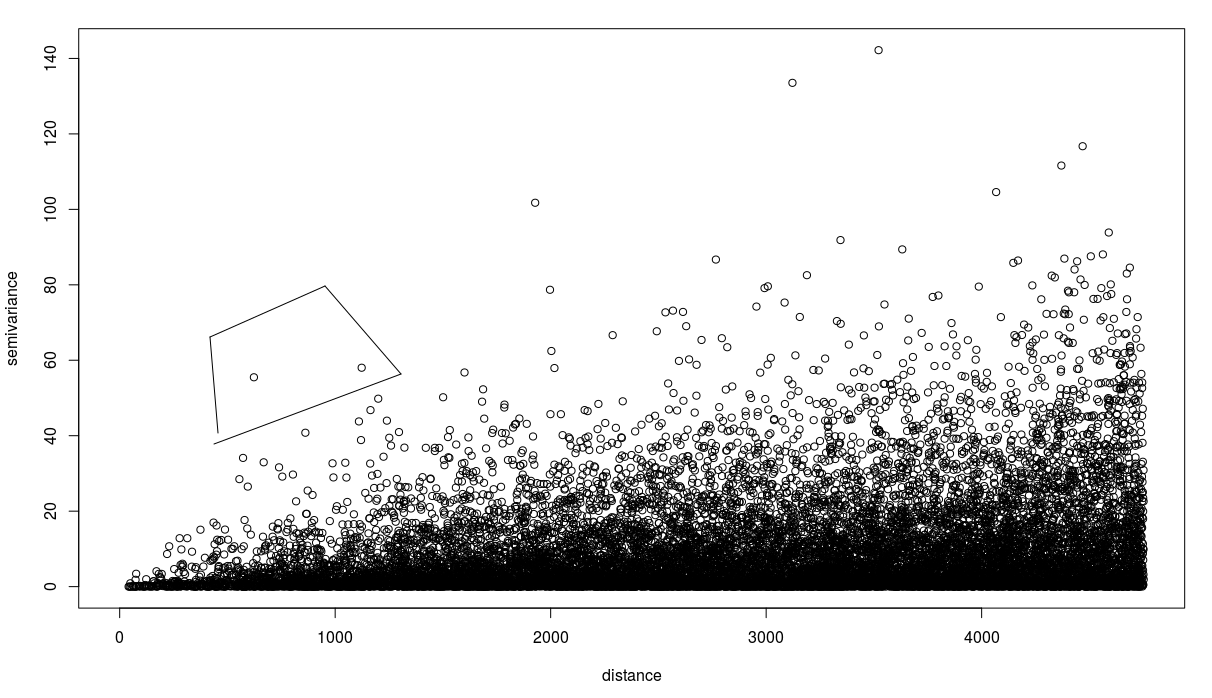
\includegraphics[width=1\linewidth]{figs/cloud_sel} 

}

\caption{Przykład wyboru par odstających z chmury semiwariogramu zmiennej temp.}\label{fig:06-semiwariancja-8}
\end{figure}

Następnie można wyświetlić wybrane pary punktów z użyciem funkcji \texttt{plot()} (rycina \ref{fig:06-semiwariancja-9}).

\begin{Shaded}
\begin{Highlighting}[]
\FunctionTok{plot}\NormalTok{(vario\_cloud\_sel, punkty)}
\end{Highlighting}
\end{Shaded}

\begin{figure}

{\centering 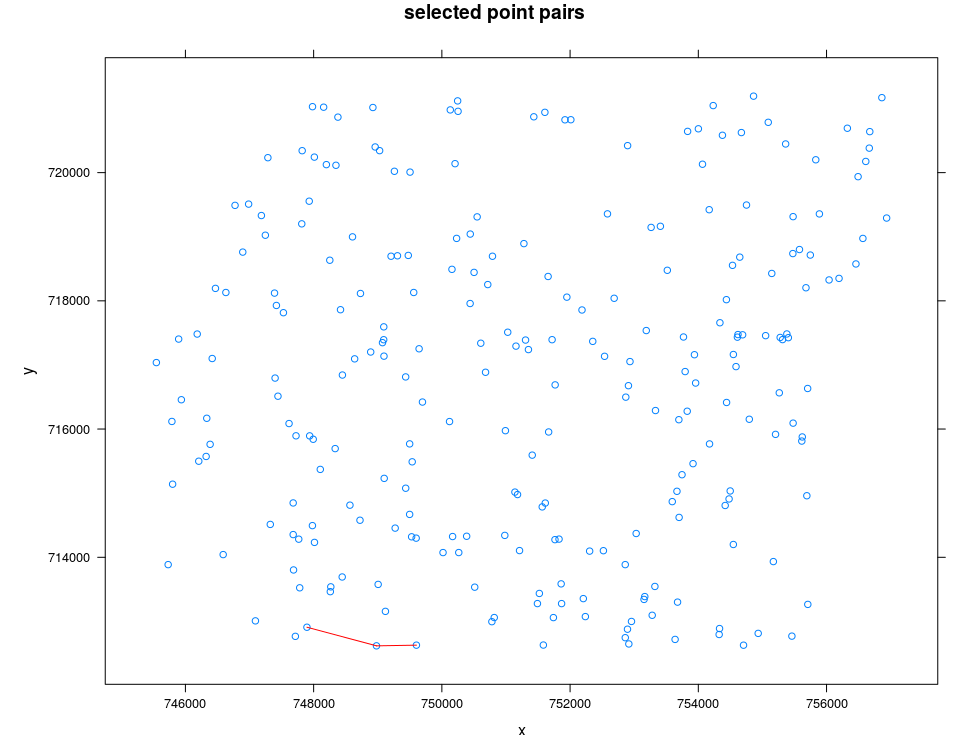
\includegraphics[width=1\linewidth]{figs/points_sel} 

}

\caption{Lokalizacja wybranych par obserwacji (czerwone linie).}\label{fig:06-semiwariancja-9}
\end{figure}

\subsection{Charakterystyka struktury przestrzennej}\label{charakterystyka-struktury-przestrzennej}

Semiwariogram jest wykresem pokazującym relację pomiędzy odległością a semiwariancją (rycina \ref{fig:06-semiwariancja-10}).
Inaczej mówiąc, dla kolejnych odstępów (lagów) wartość semiwariancji jest uśredniana i przestawiania w odniesieniu do odległości.

\[\hat{\gamma}(h) = \frac{1}{2N(h)}\sum_{\alpha=1}^{N(h)}(z(u_{\alpha}) - z(u_{\alpha}+h))^2\]

, gdzie \(N(h)\) oznacza liczbę par punktów w odstępie \(h\).

W oparciu o semiwariogram empiryczny (czyli oparty na danych) możemy następnie dopasować do niego model/e.

\begin{figure}

{\centering 
\includegraphics[width=1\linewidth]{06-semiwariancja_files/figure-latex/06-semiwariancja-10-1} 

}

\caption{Semiwariogram empiryczny zmiennej temp.}\label{fig:06-semiwariancja-10}
\end{figure}

\subsection{Tworzenie semiwariogramu}\label{tworzenie-semiwariogramu}

Stworzenie podstawowego semiwariogramu w pakiecie \textbf{gstat} odbywa się z użyciem funkcji \texttt{variogram()}.
Należy w niej zdefiniować analizowaną zmienną (w tym przykładzie \texttt{temp\ \textasciitilde{}\ 1}) oraz zbiór punktowy (\texttt{punkty}).

\begin{Shaded}
\begin{Highlighting}[]
\NormalTok{vario\_par }\OtherTok{=} \FunctionTok{variogram}\NormalTok{(temp }\SpecialCharTok{\textasciitilde{}} \DecValTok{1}\NormalTok{, }\AttributeTok{locations =}\NormalTok{ punkty)}
\NormalTok{vario\_par}
\end{Highlighting}
\end{Shaded}

\begin{verbatim}
##      np      dist     gamma dir.hor dir.ver   id
## 1   111  212.9356  1.203287       0       0 var1
## 2   283  489.0804  2.639854       0       0 var1
## 3   446  792.3222  4.226593       0       0 var1
## 4   631 1116.0957  5.187903       0       0 var1
## 5   815 1423.8256  6.352106       0       0 var1
## 6   892 1739.7600  7.186529       0       0 var1
## 7   943 2051.5149  7.598215       0       0 var1
## 8  1078 2371.6198  8.453746       0       0 var1
## 9  1218 2684.4065  9.826903       0       0 var1
## 10 1155 3002.3276  9.626642       0       0 var1
## 11 1242 3312.6962 11.642621       0       0 var1
## 12 1285 3633.4536 11.357612       0       0 var1
## 13 1302 3944.5241 11.635848       0       0 var1
## 14 1362 4261.7974 14.460067       0       0 var1
## 15 1409 4578.9006 15.480848       0       0 var1
\end{verbatim}

Do wyświetlenia semiwariogramu służy funkcja \texttt{plot()}.
Można również dodać informację o liczbie par punktów, jaka posłużyła do wyliczenia semiwariancji dla kolejnych odstępów poprzez argument \texttt{plot.numbers\ =\ TRUE} (rycina \ref{fig:06-semiwariancja-12}).

\begin{Shaded}
\begin{Highlighting}[]
\FunctionTok{plot}\NormalTok{(vario\_par, }\AttributeTok{plot.numbers =} \ConstantTok{TRUE}\NormalTok{)}
\end{Highlighting}
\end{Shaded}

\begin{figure}

{\centering 
\includegraphics[width=1\linewidth]{06-semiwariancja_files/figure-latex/06-semiwariancja-12-1} 

}

\caption{Semiwariogram empiryczny zmiennej temp wraz z zaznaczoną liczbą par dla każdego odstępu.}\label{fig:06-semiwariancja-12}
\end{figure}

\subsection{Parametry semiwariogramu}\label{parametry-semiwariogramu}

Przy ustalaniu parametrów semiwariogramu powinno się stosować do kilku utartych zasad (tzw. \emph{rules of thumb}):

\begin{itemize}
\tightlist
\item
  W każdym odstępie powinno się znaleźć co najmniej 30 par punktów.
\item
  Maksymalny zasięg semiwariogramu (ang. \emph{cutoff distance}) to 1/2 pierwiastka z badanej powierzchni (inne źródła mówią o połowie z przekątnej badanego obszaru/jednej trzeciej).
\item
  Liczba odstępów powinna nie być mniejsza niż 10.
\item
  Optymalnie maksymalny zasięg semiwariogramu powinien być dłuższy o 10-15\% od zasięgu zjawiska.
\item
  Optymalnie odstępy powinny być jak najbliżej siebie i jednocześnie nie być chaotyczne.
\item
  Warto metodą prób i błędów określić optymalne parametry semiwariogramu.
\item
  Należy określić czy zjawisko wykazuje anizotropię przestrzenną.
\end{itemize}

\subsection{Obliczenia pomocnicze}\label{obliczenia-pomocnicze}

W zrozumieniu danych oraz przy określaniu parametrów semiwariogramu może pomóc szereg obliczeń pomocniczych.
Przykładowo, aby wyliczyć liczbę par obserwacji można użyć poniższego kodu.

\begin{Shaded}
\begin{Highlighting}[]
\FloatTok{0.5} \SpecialCharTok{*} \FunctionTok{nrow}\NormalTok{(punkty) }\SpecialCharTok{*}\NormalTok{ (}\FunctionTok{nrow}\NormalTok{(punkty) }\SpecialCharTok{{-}} \DecValTok{1}\NormalTok{)}
\end{Highlighting}
\end{Shaded}

\begin{verbatim}
## [1] 29161
\end{verbatim}

Powierzchnia zajmowana przez jedną próbkę jest osiągana poprzez podzielenie całej badanej powierzchni poprzez liczbę punktów.

\begin{Shaded}
\begin{Highlighting}[]
\NormalTok{pow\_pr }\OtherTok{=} \FunctionTok{st\_area}\NormalTok{(granica) }\SpecialCharTok{/} \FunctionTok{nrow}\NormalTok{(punkty)}
\NormalTok{pow\_pr}
\end{Highlighting}
\end{Shaded}

\begin{verbatim}
## 261886.9 [m^2]
\end{verbatim}

Średnia odległość między punktami to wartość pierwiastka z powierzchni zajmowanej przez jedną próbkę.

\begin{Shaded}
\begin{Highlighting}[]
\FunctionTok{sqrt}\NormalTok{(pow\_pr)}
\end{Highlighting}
\end{Shaded}

\begin{verbatim}
## 511.7489 [m]
\end{verbatim}

Ostatnim obliczeniem pomocniczym jest określenie połowy pierwiastka powierzchni.
Może być ono następnie użyte do ustalenia maksymalnego zasięgu semiwariogramu.

\begin{Shaded}
\begin{Highlighting}[]
\NormalTok{pow }\OtherTok{=} \FunctionTok{st\_area}\NormalTok{(granica)}
\FloatTok{0.5} \SpecialCharTok{*} \FunctionTok{sqrt}\NormalTok{(pow)}
\end{Highlighting}
\end{Shaded}

\begin{verbatim}
## 3980.472 [m]
\end{verbatim}

\subsection{Modyfikacja semiwariogramu}\label{modyfikacja-semiwariogramu}

Maksymalny zasięg semiwariogramu (ang. \emph{cutoff distance}) jest domyślnie wyliczany w pakiecie \textbf{gstat} jako 1/3 z najdłuższej przekątnej badanego obszaru.
Można jednak tę wartość zmodyfikować używając argumentu \texttt{cutoff} (rycina \ref{fig:06-semiwariancja-18}).

\begin{Shaded}
\begin{Highlighting}[]
\NormalTok{vario\_par }\OtherTok{=} \FunctionTok{variogram}\NormalTok{(temp }\SpecialCharTok{\textasciitilde{}} \DecValTok{1}\NormalTok{, }\AttributeTok{locations =}\NormalTok{ punkty,}
                      \AttributeTok{cutoff =} \DecValTok{4000}\NormalTok{)}
\FunctionTok{plot}\NormalTok{(vario\_par)}
\end{Highlighting}
\end{Shaded}

\begin{figure}

{\centering 
\includegraphics[width=1\linewidth]{06-semiwariancja_files/figure-latex/06-semiwariancja-18-1} 

}

\caption{Semiwariogram empiryczny zmiennej temp używając ręcznie ustalonej wartości maksymalnego zasięgu semiwariogramu.}\label{fig:06-semiwariancja-18}
\end{figure}

Dodatkowo, domyślnie w pakiecie \textbf{gstat} odległość między przedziałami (ang. \emph{interval width}) jest wyliczana jako maksymalny zasięg semiwariogramu podzielony przez 15.
Można to oczywiście zmienić używając zarówno argumentu \texttt{cutoff}, jak i argumentu \texttt{width} mówiącego o szerokości odstępów (rycina \ref{fig:06-semiwariancja-19}).

\begin{Shaded}
\begin{Highlighting}[]
\NormalTok{vario\_par }\OtherTok{=} \FunctionTok{variogram}\NormalTok{(temp }\SpecialCharTok{\textasciitilde{}} \DecValTok{1}\NormalTok{, }\AttributeTok{locations =}\NormalTok{ punkty,}
                      \AttributeTok{cutoff =} \DecValTok{4000}\NormalTok{, }\AttributeTok{width =} \DecValTok{100}\NormalTok{)}
\FunctionTok{plot}\NormalTok{(vario\_par)}
\end{Highlighting}
\end{Shaded}

\begin{figure}

{\centering 
\includegraphics[width=1\linewidth]{06-semiwariancja_files/figure-latex/06-semiwariancja-19-1} 

}

\caption{Semiwariogram empiryczny zmiennej temp używając ręcznie ustalonej wartości szerokości odstępów.}\label{fig:06-semiwariancja-19}
\end{figure}

\section{Anizotropia}\label{anizotropia}

\subsection{Anizotropia struktury przestrzennej}\label{anizotropia-struktury-przestrzennej}

W wielu sytuacjach, podobieństwo pomiędzy wartość cechy w punktach zależy nie tylko od odległości, ale także od kierunku.
O takim zjawisku mówimy, że wykazuje ono anizotropię struktury przestrzennej.

\subsection{Mapa semiwariogramu}\label{mapa-semiwariogramu}

Mapa semiwariogramu (zwana inaczej powierzchnią semiwariogramu) służy do określenia czy struktura przestrzenna zjawiska posiada anizotropię, a jeżeli tak to w jakim kierunku.
Na podstawie mapy semiwariogramu identyfikuje się także parametry potrzebne do zbudowania semiwariogramów kierunkowych.

Stworzenie mapy semiwariogramu odbywa się poprzez dodanie kilku argumentów do funkcji \texttt{variogram()}: oprócz argumentu zmiennej i zbioru punktowego, jest to \texttt{cutoff}, \texttt{width}, oraz \texttt{map\ =\ TRUE}.
Następnie można ją wyświetlić używając funkcji \texttt{plot()} (rycina \ref{fig:06-semiwariancja-21}).
Warto w tym wypadku użyć dodatkowego argumentu \texttt{threshold}, który powoduje, że niepewna wartość semiwariancji (wyliczona na małej liczbie punktów) nie jest wyświetlana.

\begin{Shaded}
\begin{Highlighting}[]
\NormalTok{vario\_map }\OtherTok{=} \FunctionTok{variogram}\NormalTok{(temp }\SpecialCharTok{\textasciitilde{}} \DecValTok{1}\NormalTok{, }\AttributeTok{locations =}\NormalTok{ punkty, }
                      \AttributeTok{cutoff =} \DecValTok{4000}\NormalTok{, }\AttributeTok{width =} \DecValTok{400}\NormalTok{, }\AttributeTok{map =} \ConstantTok{TRUE}\NormalTok{)}
\CommentTok{\# co najmniej 30 par punktów}
\FunctionTok{plot}\NormalTok{(vario\_map, }\AttributeTok{threshold =} \DecValTok{30}\NormalTok{,}
     \AttributeTok{col.regions =} \FunctionTok{hcl.colors}\NormalTok{(}\DecValTok{40}\NormalTok{, }\AttributeTok{palette =} \StringTok{"ag\_GrnYl"}\NormalTok{, }\AttributeTok{rev =} \ConstantTok{TRUE}\NormalTok{)) }
\end{Highlighting}
\end{Shaded}

\begin{figure}

{\centering 
\includegraphics[width=1\linewidth]{06-semiwariancja_files/figure-latex/06-semiwariancja-21-1} 

}

\caption{Mapa semiwariogramu zmiennej temp.}\label{fig:06-semiwariancja-21}
\end{figure}

\subsection{Semiwariogramy kierunkowe}\label{semiwariogramy-kierunkowe}

W przypadku, gdy zjawisko wykazuje anizotropię przestrzenną, możliwe jest stworzenie semiwariogramów dla różnych wybranych kierunków (rycina \ref{fig:06-semiwariancja-22}).
Dla argumentu \texttt{alpha\ =\ c(0,\ 45,\ 90,\ 135)} wybrane cztery główne kierunki to 0, 45, 90 i 135 stopni.
Oznacza to, że przykładowo dla kierunku 45 stopni brane pod uwagę będą wszystkie pary punktów pomiędzy 22,5 a 67,5 stopnia.

\begin{Shaded}
\begin{Highlighting}[]
\NormalTok{vario\_kier }\OtherTok{=} \FunctionTok{variogram}\NormalTok{(temp }\SpecialCharTok{\textasciitilde{}} \DecValTok{1}\NormalTok{, }\AttributeTok{locations =}\NormalTok{ punkty, }
                        \AttributeTok{alpha =} \FunctionTok{c}\NormalTok{(}\DecValTok{0}\NormalTok{, }\DecValTok{45}\NormalTok{, }\DecValTok{90}\NormalTok{, }\DecValTok{135}\NormalTok{))}
\FunctionTok{plot}\NormalTok{(vario\_kier)}
\end{Highlighting}
\end{Shaded}

\begin{figure}

{\centering 
\includegraphics[width=1\linewidth]{06-semiwariancja_files/figure-latex/06-semiwariancja-22-1} 

}

\caption{Semiwariogramy kierunkowe dla zmiennej temp.}\label{fig:06-semiwariancja-22}
\end{figure}

\section{Zadania}\label{z6}

Przyjrzyj się~danym z obiektu \texttt{punkty\_pref}.
Możesz go wczytać używając poniższego kodu:

\begin{Shaded}
\begin{Highlighting}[]
\FunctionTok{data}\NormalTok{(punkty\_pref)}
\end{Highlighting}
\end{Shaded}

\begin{enumerate}
\def\labelenumi{\arabic{enumi}.}
\item
  Stwórz wykres rozrzutu z przesunięciem dla zmiennej \texttt{srtm} dla odstępów od 0 do 5000 metrów co 625 metry.
  Co można odczytać z otrzymanego wykresu?
\item
  Wylicz odległość oraz wartość semiwariancji dla zmiennej \texttt{srtm} pomiędzy pierwszym i drugim, pierwszym i trzecim, oraz drugim i trzecim punktem.
  Zwizualizuj te trzy punkty.
  W jaki sposób można zinterpretować otrzymane wyniki wartości semiwariancji?
\item
  Twórz chmurę semiwariogramu dla zmiennej \texttt{temp}.
  W jaki sposób można zaobserwować na niej wartości odstające?
  Co one oznaczają?
\item
  Jaka jest liczba par obserwacji, średnia powierzchnia zajmowana przez jedną próbkę (w km\textsuperscript{2}) oraz średnia odległość między punktami (w km)?
\item
  Stwórz semiwariogram zmiennej \texttt{srtm}.
  Ile par punktów posłużyło do wyliczenia pierwszego odstępu?
\item
  Zmodyfikuj powyższy semiwariogram, żeby jego maksymalny zasięg wynosił 3,5 kilometra.
\item
  Stwórz mapę semiwariogramu dla zmiennej \texttt{srtm}.
  Sprawdź różne wartości \texttt{cutoff} (od 3 do 5 km) oraz \texttt{width} (od 200 do 500 metrów).
  Zmień domyślną paletę kolorów w wizualizacji mapy semiwariogramu.
  (Dodatkowe: spróbuj do tego celu użyć pakietu \textbf{viridisLite}).
\item
  Co przedstawia stworzona mapa semiwariogramu?
  Czy badane zjawisko wykazuje izotropię czy anizotropię?
\item
  Jeżeli mapa semiwariogramu wykazuje anizotropię struktury przestrzennej to w jakim kierunku?
  Stwórz semiwariogramy dla wybranych kierunków.
\end{enumerate}

\chapter{Modelowanie autokorelacji przestrzennej}\label{modelowanie-matematycznie-autokorelacji-przestrzennej}

Odtworzenie obliczeń z tego rozdziału wymaga załączenia poniższych pakietów oraz wczytania poniższych danych:

\begin{Shaded}
\begin{Highlighting}[]
\FunctionTok{library}\NormalTok{(sf)}
\FunctionTok{library}\NormalTok{(stars)}
\FunctionTok{library}\NormalTok{(gstat)}
\FunctionTok{library}\NormalTok{(geostatbook)}
\FunctionTok{data}\NormalTok{(punkty)}
\end{Highlighting}
\end{Shaded}

\section{Modelowanie matematycznie autokorelacji przestrzennej}\label{modelowanie-matematycznie-autokorelacji-przestrzennej-1}

\subsection{Modelowanie struktury przestrzennej}\label{modelowanie-struktury-przestrzennej}

Semiwariogram empiryczny (wyliczony z danych punktowych) jest:

\begin{itemize}
\tightlist
\item
  Nieciągły - wartości semiwariancji są średnimi przedziałowymi.
\item
  Chaotyczny - badana próba jest jedynie przybliżeniem rzeczywistości, dodatkowo obciążonym błędami.
\end{itemize}

Estymacje i symulacje przestrzenne wymagają modelu struktury przestrzennej analizowanej cechy, a nie tylko wartości empirycznych.
Dodatkowo, matematycznie modelowanie wygładza chaotyczne fluktuacje danych empirycznych (rycina \ref{fig:07-modelowanie-3}).

\begin{figure}

{\centering 
\includegraphics[width=1\linewidth]{07-modelowanie_files/figure-latex/07-modelowanie-3-1} 

}

\caption{Porównanie semiwariogramu empirycznego i modelu semiwariogramu.}\label{fig:07-modelowanie-3}
\end{figure}

\subsection{Model semiwariogramu}\label{model-semiwariogramu}

Model semiwariogramu składa się zazwyczaj z trzech podstawowych elementów (rycina \ref{fig:07-modelowanie-4}).
Są to:

\begin{itemize}
\tightlist
\item
  \textbf{Nugget} - efekt nuggetowy - pozwala na określenie błędu w danych wejściowych oraz zmienności na dystansie krótszym niż pierwszy odstęp.
\item
  \textbf{Sill} - semiwariancja progowa - oznacza wariancję badanej zmiennej.
\item
  \textbf{Range} - zasięg - to odległość do której istnieje przestrzenna korelacja.
\end{itemize}

\begin{figure}

{\centering 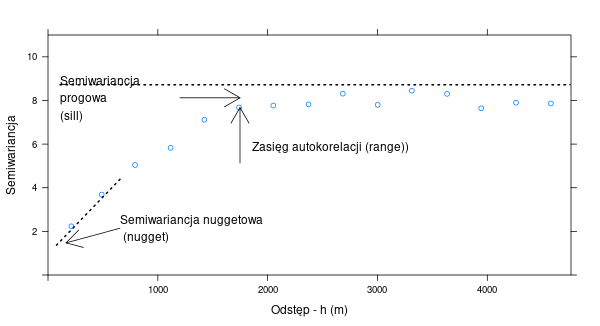
\includegraphics[width=1\linewidth]{figs/variogram_text} 

}

\caption{Podstawowe elementy modelu semiwariogramu.}\label{fig:07-modelowanie-4}
\end{figure}

\subsection{Model nuggetowy}\label{model-nuggetowy}

Model nuggetowy określa sytuację, w której analizowana zmienna nie wykazuje autokorelacji.
Inaczej mówiąc, niepodobieństwo jej wartości nie wzrasta wraz z odległością.
Model nuggetowy nie powinien być używany samodzielnie - w większości zastosowań jest on elementem modelu złożonego.
Służy on do określania, między innymi, błędu pomiarowego czy zmienności na krótkich odstępach.

\section{Modele podstawowe}\label{modele-podstawowe}

\subsection{Typy modeli podstawowych}\label{typy-modeli-podstawowych}

Pakiet \texttt{gstat} zawiera 20 podstawowych modeli geostatystycznych, w tym najczęściej używane takie jak:

\begin{itemize}
\tightlist
\item
  Nuggetowy (ang. \emph{Nugget effect model})
\item
  Sferyczny (ang. \emph{Spherical model})
\item
  Gaussowski (ang. \emph{Gaussian model})
\item
  Potęgowy (ang. \emph{Power model})
\item
  Wykładniczy (ang. \emph{Exponential model})
\item
  Inne
\end{itemize}

Do wyświetlenia listy nazw modeli i ich skrótów służy funkcja \texttt{vgm()}.

\begin{Shaded}
\begin{Highlighting}[]
\FunctionTok{vgm}\NormalTok{()}
\end{Highlighting}
\end{Shaded}

\begin{verbatim}
##    short                                      long
## 1    Nug                              Nug (nugget)
## 2    Exp                         Exp (exponential)
## 3    Sph                           Sph (spherical)
## 4    Gau                            Gau (gaussian)
## 5    Exc        Exclass (Exponential class/stable)
## 6    Mat                              Mat (Matern)
## 7    Ste Mat (Matern, M. Stein's parameterization)
## 8    Cir                            Cir (circular)
## 9    Lin                              Lin (linear)
## 10   Bes                              Bes (bessel)
## 11   Pen                      Pen (pentaspherical)
## 12   Per                            Per (periodic)
## 13   Wav                                Wav (wave)
## 14   Hol                                Hol (hole)
## 15   Log                         Log (logarithmic)
## 16   Pow                               Pow (power)
## 17   Spl                              Spl (spline)
## 18   Leg                            Leg (Legendre)
## 19   Err                   Err (Measurement error)
## 20   Int                           Int (Intercept)
\end{verbatim}

Można się również im przyjrzeć używając funkcji \texttt{show.vgms()} (rycina \ref{fig:07-modelowanie-6}).

\begin{Shaded}
\begin{Highlighting}[]
\FunctionTok{show.vgms}\NormalTok{()}
\end{Highlighting}
\end{Shaded}

\begin{figure}

{\centering 
\includegraphics[width=1\linewidth]{07-modelowanie_files/figure-latex/07-modelowanie-6-1} 

}

\caption{Przykład modeli semiwariogramu dostępnych w pakiecie gstat.}\label{fig:07-modelowanie-6}
\end{figure}

Istnieje możliwość wyświetlenia tylko wybranych modeli podstawowych poprzez argument \texttt{models} (rycina \ref{fig:07-modelowanie-7}).

\begin{Shaded}
\begin{Highlighting}[]
\FunctionTok{show.vgms}\NormalTok{(}\AttributeTok{models =} \FunctionTok{c}\NormalTok{(}\StringTok{"Sph"}\NormalTok{, }\StringTok{"Gau"}\NormalTok{, }\StringTok{"Pow"}\NormalTok{, }\StringTok{"Exp"}\NormalTok{), }
          \AttributeTok{range =} \FloatTok{1.4}\NormalTok{, }\AttributeTok{max =} \FloatTok{2.5}\NormalTok{)}
\end{Highlighting}
\end{Shaded}

\begin{figure}

{\centering 
\includegraphics[width=1\linewidth]{07-modelowanie_files/figure-latex/07-modelowanie-7-1} 

}

\caption{Porównanie modeli sferycznego (Sph), gaussowskiego (Gau), potęgowego (Pow) i wykładniczego (Exp).}\label{fig:07-modelowanie-7}
\end{figure}

Dodatkowo, można je porównać na jednym wykresie poprzez argument \texttt{as.groups\ =\ TRUE} (rycina \ref{fig:07-modelowanie-8}).

\begin{Shaded}
\begin{Highlighting}[]
\FunctionTok{show.vgms}\NormalTok{(}\AttributeTok{models =} \FunctionTok{c}\NormalTok{(}\StringTok{"Sph"}\NormalTok{, }\StringTok{"Gau"}\NormalTok{, }\StringTok{"Pow"}\NormalTok{, }\StringTok{"Exp"}\NormalTok{), }
          \AttributeTok{range =} \FloatTok{1.4}\NormalTok{, }\AttributeTok{max =} \FloatTok{2.5}\NormalTok{, }\AttributeTok{as.groups =} \ConstantTok{TRUE}\NormalTok{)}
\end{Highlighting}
\end{Shaded}

\begin{figure}

{\centering 
\includegraphics[width=1\linewidth]{07-modelowanie_files/figure-latex/07-modelowanie-8-1} 

}

\caption{Porównanie modeli sferycznego (Sph), gaussowskiego (Gau), potęgowego (Pow) i wykładniczego (Exp) na jednym wykresie.}\label{fig:07-modelowanie-8}
\end{figure}

\section{Metody modelowania}\label{metody-modelowania}

\subsection{Rodzaje metod modelowania}\label{rodzaje-metod-modelowania}

Istnieją trzy najczęściej spotykane metody modelowania geostatystycznego:

\begin{itemize}
\tightlist
\item
  Ustawianie ``ręczne'' parametrów modelu, np. funkcja \texttt{vgm()} z pakietu \textbf{gstat}.
\item
  Ustawianie ``wizualne'' parametrów modelu, np. funkcja \texttt{eyefit()} z pakietu \textbf{geoR}.
\item
  Automatyczny wybór parametrów na podstawie różnych kryteriów statystycznych, np. funkcja \texttt{fit.variogram()} z pakietu \textbf{gstat}, \texttt{variofit()} z pakietu \textbf{geoR}, \texttt{autofitVariogram()} z pakietu \textbf{automap}.
\end{itemize}

Odpowiednie określenie modelu matematycznego często nie jest proste.
W efekcie automatyczne metody nie zawsze są w stanie dać lepszy wynik od modelowania ``ręcznego''.
Najlepiej, gdy wybór modelu oparty jest o wiedzę na temat zakładanego procesu przestrzennego.

\subsection{\texorpdfstring{Funkcja \texttt{fit.variogram()}}{Funkcja fit.variogram()}}\label{funkcja-fit.variogram}

Funkcja \texttt{fit.variogram()} z pakietu \textbf{gstat} dopasowuje zasięg oraz semiwariancję progową w oparciu o ustalone ``ręcznie'' wejściowe parametry modelu\footnote{Więcej na temat działania tej funkcji można przeczytać we wpisie na stronie \url{https://www.r-spatial.org/r/2016/02/14/gstat-variogram-fitting.html}.}.

\section{Modelowanie izotropowe}\label{modelowanie-izotropowe}

Do zbudowania modelu semiwariogramu należy wykonać szereg kroków:

\begin{enumerate}
\def\labelenumi{\arabic{enumi}.}
\tightlist
\item
  Stworzyć i wyświetlić semiwariogram empiryczny analizowanej zmiennej z użyciem funkcji \texttt{variogram()} oraz \texttt{plot()}.
\item
  Zdefiniować wejściowe parametry semiwariogramu.
  W najprostszej sytuacji wystarczy zdefiniować używany model/e poprzez skróconą nazwę używanej funkcji (\texttt{model}).
  Możliwe, ale nie wymagane jest także określenie wejściowej semiwariancji cząstkowej (\texttt{psill}) oraz zasięgu modelu (\texttt{range}) w funkcji \texttt{vgm()}.
  Uzyskany model można przedstawić w funkcji \texttt{plot()} podając nazwę obiektu zawierającego semiwariogram empiryczny oraz obiektu zawierającego model.
\item
  Dopasować parametry modelu używając funkcji \texttt{fit.variogram()}.
  To dopasowanie można również zwizualizować używając funkcji \texttt{plot()}.
\end{enumerate}

\subsection{Model sferyczny}\label{model-sferyczny}

Model sferyczny (\texttt{Sph}) jest jednym z najczęściej stosowanych modeli geostatystycznych.
Reprezentuje on cechę, której zmienność wartości ma charakter naprzemiennych płatów niskich i wysokich wartości (rycina \ref{fig:07-modelowanie-10}).
Średnio te płaty mają średnicę określoną przez zasięg (\texttt{range}) modelu.

\begin{figure}

{\centering 
\includegraphics[width=1\linewidth]{07-modelowanie_files/figure-latex/07-modelowanie-10-1} 

}

\caption{Przykład zjawiska reprezentowanego poprzez model sferyczny.}\label{fig:07-modelowanie-10}
\end{figure}

Stworzenie takiego modelu dla zmiennej \texttt{temp} polega najpierw na zbudowaniu semiwariogramu empirycznego używając funkcji \texttt{variogram()} (rycina \ref{fig:07-modelowanie-11}).

\begin{Shaded}
\begin{Highlighting}[]
\NormalTok{vario }\OtherTok{=} \FunctionTok{variogram}\NormalTok{(temp }\SpecialCharTok{\textasciitilde{}} \DecValTok{1}\NormalTok{, }\AttributeTok{locations =}\NormalTok{ punkty)}
\FunctionTok{plot}\NormalTok{(vario)}
\end{Highlighting}
\end{Shaded}

\begin{figure}

{\centering 
\includegraphics[width=1\linewidth]{07-modelowanie_files/figure-latex/07-modelowanie-11-1} 

}

\caption{Semiwariogram zmiennej temp.}\label{fig:07-modelowanie-11}
\end{figure}

W kolejnym kroku, przy użyciu funkcji \texttt{vgm()} określa się~typ modelu oraz jego podstawowe parametry (rycina \ref{fig:07-modelowanie-12}).

\begin{Shaded}
\begin{Highlighting}[]
\NormalTok{model\_sph }\OtherTok{=} \FunctionTok{vgm}\NormalTok{(}\AttributeTok{psill =} \DecValTok{10}\NormalTok{, }\AttributeTok{model =} \StringTok{"Sph"}\NormalTok{, }\AttributeTok{range =} \DecValTok{3000}\NormalTok{)}
\NormalTok{model\_sph}
\end{Highlighting}
\end{Shaded}

\begin{verbatim}
##   model psill range
## 1   Sph    10  3000
\end{verbatim}

\begin{Shaded}
\begin{Highlighting}[]
\FunctionTok{plot}\NormalTok{(vario, }\AttributeTok{model =}\NormalTok{ model\_sph)}
\end{Highlighting}
\end{Shaded}

\begin{figure}

{\centering 
\includegraphics[width=1\linewidth]{07-modelowanie_files/figure-latex/07-modelowanie-12-1} 

}

\caption{Model sferyczny zmiennej temp.}\label{fig:07-modelowanie-12}
\end{figure}

Dodatkowo możliwe jest także automatyczne dopasowanie modelu w oparciu o wstępnie podane parametry używając funkcji \texttt{fit.variogram()} (rycina \ref{fig:07-modelowanie-13}).

\begin{Shaded}
\begin{Highlighting}[]
\NormalTok{fitted\_sph }\OtherTok{=} \FunctionTok{fit.variogram}\NormalTok{(vario, model\_sph)}
\NormalTok{fitted\_sph}
\end{Highlighting}
\end{Shaded}

\begin{verbatim}
##   model    psill    range
## 1   Sph 13.20295 4549.691
\end{verbatim}

\begin{Shaded}
\begin{Highlighting}[]
\FunctionTok{plot}\NormalTok{(vario, }\AttributeTok{model =}\NormalTok{ fitted\_sph)}
\end{Highlighting}
\end{Shaded}

\begin{figure}

{\centering 
\includegraphics[width=1\linewidth]{07-modelowanie_files/figure-latex/07-modelowanie-13-1} 

}

\caption{Automatycznie dopasowany model sferyczny zmiennej temp używając wstępnie podanych parametrów.}\label{fig:07-modelowanie-13}
\end{figure}

W niektórych przypadkach funkcja \texttt{fit.variogram()} da także zadowalające wyniki, gdy tylko zostanie podany typ modelu (rycina \ref{fig:07-modelowanie-14}).

\begin{Shaded}
\begin{Highlighting}[]
\NormalTok{model\_sph2 }\OtherTok{=} \FunctionTok{vgm}\NormalTok{(}\AttributeTok{model =} \StringTok{"Sph"}\NormalTok{)}
\NormalTok{fitted\_sph2 }\OtherTok{=} \FunctionTok{fit.variogram}\NormalTok{(vario, model\_sph2)}
\NormalTok{fitted\_sph2}
\end{Highlighting}
\end{Shaded}

\begin{verbatim}
##   model   psill    range
## 1   Sph 13.2018 4549.092
\end{verbatim}

\begin{Shaded}
\begin{Highlighting}[]
\FunctionTok{plot}\NormalTok{(vario, }\AttributeTok{model =}\NormalTok{ fitted\_sph2)}
\end{Highlighting}
\end{Shaded}

\begin{figure}

{\centering 
\includegraphics[width=1\linewidth]{07-modelowanie_files/figure-latex/07-modelowanie-14-1} 

}

\caption{Automatycznie dopasowany model sferyczny zmiennej temp używając jedynie wstępnie podanego typu modelu.}\label{fig:07-modelowanie-14}
\end{figure}

\subsection{Model wykładniczy}\label{model-wykux142adniczy}

Model wykładniczy (\texttt{Exp}) również jest jednym z najczęściej używanych w geostatystyce.
Od modelu sferycznego różni go szczególnie to, że nie ma on skończonego zasięgu.
W jego przypadku, zamiast zasięgu podaje się tzw. zasięg praktyczny.
Oznacza on odległość na jakiej model osiąga 95\% wartości wariancji progowej (rycina \ref{fig:07-modelowanie-15}).

\begin{figure}

{\centering 
\includegraphics[width=1\linewidth]{07-modelowanie_files/figure-latex/07-modelowanie-15-1} 

}

\caption{Przykład zjawiska reprezentowanego poprzez model wykładniczy.}\label{fig:07-modelowanie-15}
\end{figure}

Proces tworzenia tego modelu jest bardzo podobny do przedstawionego powyżej - budowany jest semiwariogram empiryczny, a następnie ustalany jest model poprzez podanie kilku jego parametrów (rycina \ref{fig:07-modelowanie-17}).

\begin{Shaded}
\begin{Highlighting}[]
\NormalTok{vario }\OtherTok{=} \FunctionTok{variogram}\NormalTok{(temp }\SpecialCharTok{\textasciitilde{}} \DecValTok{1}\NormalTok{, }\AttributeTok{locations =}\NormalTok{ punkty)}
\CommentTok{\# plot(vario)}
\NormalTok{model\_exp }\OtherTok{=} \FunctionTok{vgm}\NormalTok{(}\AttributeTok{psill =} \DecValTok{10}\NormalTok{, }\AttributeTok{model =} \StringTok{"Exp"}\NormalTok{, }\AttributeTok{range =} \DecValTok{3000}\NormalTok{)}
\NormalTok{model\_exp}
\end{Highlighting}
\end{Shaded}

\begin{verbatim}
##   model psill range
## 1   Exp    10  3000
\end{verbatim}

\begin{Shaded}
\begin{Highlighting}[]
\FunctionTok{plot}\NormalTok{(vario, }\AttributeTok{model =}\NormalTok{ model\_exp)}
\end{Highlighting}
\end{Shaded}

\begin{figure}

{\centering 
\includegraphics[width=1\linewidth]{07-modelowanie_files/figure-latex/07-modelowanie-17-1} 

}

\caption{Model wykładniczy zmiennej temp.}\label{fig:07-modelowanie-17}
\end{figure}

Dalej, funkcja \texttt{fit.variogram()} może pomóc w dopasowaniu tego modelu (rycina \ref{fig:07-modelowanie-18}).

\begin{Shaded}
\begin{Highlighting}[]
\NormalTok{fitted\_exp }\OtherTok{=} \FunctionTok{fit.variogram}\NormalTok{(vario, model\_exp)}
\NormalTok{fitted\_exp}
\end{Highlighting}
\end{Shaded}

\begin{verbatim}
##   model    psill    range
## 1   Exp 17.87051 3298.917
\end{verbatim}

\begin{Shaded}
\begin{Highlighting}[]
\FunctionTok{plot}\NormalTok{(vario, }\AttributeTok{model =}\NormalTok{ fitted\_exp)}
\end{Highlighting}
\end{Shaded}

\begin{figure}

{\centering 
\includegraphics[width=1\linewidth]{07-modelowanie_files/figure-latex/07-modelowanie-18-1} 

}

\caption{Automatycznie dopasowany model wykładniczy zmiennej temp.}\label{fig:07-modelowanie-18}
\end{figure}

\subsection{Model gaussowski}\label{model-gaussowski}

Model gaussowski (\texttt{Gau}) również posiada zasięg praktyczny definiowany jako 95\% wartości wariancji progowej (rycina \ref{fig:07-modelowanie-19}).
Jego cechą charakterystyczną jest paraboliczny kształt na początkowym odcinku.
Jest on najczęściej używany do modelowania cech o regularnej i łagodnej zmienności przestrzennej.
Model gaussowski z uwagi na swoje cechy zazwyczaj nie powinien być stosowany samodzielnie, lecz jako element modelu złożonego.

\begin{figure}

{\centering 
\includegraphics[width=1\linewidth]{07-modelowanie_files/figure-latex/07-modelowanie-19-1} 

}

\caption{Przykład zjawiska reprezentowanego poprzez model gaussowski.}\label{fig:07-modelowanie-19}
\end{figure}

Zdefiniowanie modelu gaussowskiego odbywa się używając skrótu \texttt{"Gau"} (rycina \ref{fig:07-modelowanie-21}).

\begin{Shaded}
\begin{Highlighting}[]
\NormalTok{vario }\OtherTok{=} \FunctionTok{variogram}\NormalTok{(temp }\SpecialCharTok{\textasciitilde{}} \DecValTok{1}\NormalTok{, }\AttributeTok{locations =}\NormalTok{ punkty)}
\CommentTok{\# plot(vario)}
\NormalTok{model\_gau }\OtherTok{=} \FunctionTok{vgm}\NormalTok{(}\AttributeTok{psill =} \DecValTok{13}\NormalTok{, }\AttributeTok{model =} \StringTok{"Gau"}\NormalTok{, }\AttributeTok{range =} \DecValTok{3000}\NormalTok{)}
\NormalTok{model\_gau}
\end{Highlighting}
\end{Shaded}

\begin{verbatim}
##   model psill range
## 1   Gau    13  3000
\end{verbatim}

\begin{Shaded}
\begin{Highlighting}[]
\FunctionTok{plot}\NormalTok{(vario, }\AttributeTok{model =}\NormalTok{ model\_gau)}
\end{Highlighting}
\end{Shaded}

\begin{figure}

{\centering 
\includegraphics[width=1\linewidth]{07-modelowanie_files/figure-latex/07-modelowanie-21-1} 

}

\caption{Model gaussowski zmiennej temp.}\label{fig:07-modelowanie-21}
\end{figure}

Dopasowanie tego modelu może również nastąpić używając funkcji \texttt{fit.variogram()} (rycina \ref{fig:07-modelowanie-22}).

\begin{Shaded}
\begin{Highlighting}[]
\NormalTok{fitted\_gau }\OtherTok{=} \FunctionTok{fit.variogram}\NormalTok{(vario, model\_gau)}
\NormalTok{fitted\_gau}
\end{Highlighting}
\end{Shaded}

\begin{verbatim}
##   model    psill    range
## 1   Gau 8.573835 852.2404
\end{verbatim}

\begin{Shaded}
\begin{Highlighting}[]
\FunctionTok{plot}\NormalTok{(vario, }\AttributeTok{model =}\NormalTok{ fitted\_gau)}
\end{Highlighting}
\end{Shaded}

\begin{figure}

{\centering 
\includegraphics[width=1\linewidth]{07-modelowanie_files/figure-latex/07-modelowanie-22-1} 

}

\caption{Automatycznie dopasowany model gaussowski zmiennej temp.}\label{fig:07-modelowanie-22}
\end{figure}

\subsection{Model potęgowy}\label{model-potux119gowy}

Model potęgowy (\texttt{Pow}) to przykład tzw. modelu nieograniczonego (rycina \ref{fig:07-modelowanie-23}).
Jego wartość rośnie w nieskończoność, dlatego niemożliwe jest określenie jego zasięgu.
W przypadku modelu potęgowego, parametr \texttt{range} oznacza wykładnik potęgowy.

\begin{figure}

{\centering 
\includegraphics[width=1\linewidth]{07-modelowanie_files/figure-latex/07-modelowanie-23-1} 

}

\caption{Przykład zjawiska reprezentowanego poprzez model potęgowy.}\label{fig:07-modelowanie-23}
\end{figure}

Model potęgowy jest określany skrótem \texttt{"Pow"} (ryciny \ref{fig:07-modelowanie-25} i \ref{fig:07-modelowanie-26}).

\begin{Shaded}
\begin{Highlighting}[]
\NormalTok{vario }\OtherTok{=} \FunctionTok{variogram}\NormalTok{(temp }\SpecialCharTok{\textasciitilde{}} \DecValTok{1}\NormalTok{, }\AttributeTok{locations =}\NormalTok{ punkty)}
\CommentTok{\# plot(vario)}
\NormalTok{model\_pow }\OtherTok{=} \FunctionTok{vgm}\NormalTok{(}\AttributeTok{psill =} \FloatTok{0.03}\NormalTok{, }\AttributeTok{model =} \StringTok{"Pow"}\NormalTok{, }\AttributeTok{range =} \FloatTok{0.7}\NormalTok{)}
\NormalTok{model\_pow}
\end{Highlighting}
\end{Shaded}

\begin{verbatim}
##   model psill range
## 1   Pow  0.03   0.7
\end{verbatim}

\begin{Shaded}
\begin{Highlighting}[]
\FunctionTok{plot}\NormalTok{(vario, }\AttributeTok{model =}\NormalTok{ model\_pow)}
\end{Highlighting}
\end{Shaded}

\begin{figure}

{\centering 
\includegraphics[width=1\linewidth]{07-modelowanie_files/figure-latex/07-modelowanie-25-1} 

}

\caption{Model potęgowy zmiennej temp.}\label{fig:07-modelowanie-25}
\end{figure}

\begin{Shaded}
\begin{Highlighting}[]
\NormalTok{fitted\_pow }\OtherTok{=} \FunctionTok{fit.variogram}\NormalTok{(vario, model\_pow)}
\NormalTok{fitted\_pow}
\end{Highlighting}
\end{Shaded}

\begin{verbatim}
##   model      psill     range
## 1   Pow 0.02515946 0.7535889
\end{verbatim}

\begin{Shaded}
\begin{Highlighting}[]
\FunctionTok{plot}\NormalTok{(vario, }\AttributeTok{model =}\NormalTok{ fitted\_pow)}
\end{Highlighting}
\end{Shaded}

\begin{figure}

{\centering 
\includegraphics[width=1\linewidth]{07-modelowanie_files/figure-latex/07-modelowanie-26-1} 

}

\caption{Automatycznie dopasowany model potęgowy zmiennej temp.}\label{fig:07-modelowanie-26}
\end{figure}

\subsection{Porównanie modeli}\label{poruxf3wnanie-modeli}

Z uwagi na swoją charakterystykę, każdy z powyższych modeli ma inny zakres wartości.
Aby porównać te modele należy je przedstawić używając tej samej skali kolorystycznej (\ref{fig:07-modelowanie-27}).

\begin{figure}

{\centering 
\includegraphics[width=1\linewidth]{07-modelowanie_files/figure-latex/07-modelowanie-27-1} 

}

\caption{Porównanie powierzchni reprezentowanej przez modele sferyczny, wykładniczy, gaussowski i potęgowy.}\label{fig:07-modelowanie-27}
\end{figure}

\subsection{Modele złożone I}\label{modele-zux142oux17cone-i}

Najczęściej pojedynczy model nie jest w stanie odwzorować dokładnie zmienności przestrzennej analizowanej cechy.
W takich sytuacjach konieczne jest połączenie dwóch lub więcej modeli podstawowych.
Najbardziej powszechny model złożony składa się z funkcji nuggetowej (dla odległości zero) oraz drugiej funkcji (dla dalszej odległości) (rycina \ref{fig:07-modelowanie-28}).
Zdefiniowanie takiej funkcji odbywa się poprzez dodanie argumentu \texttt{nugget} w funkcji \texttt{vgm()}.

\begin{Shaded}
\begin{Highlighting}[]
\NormalTok{vario }\OtherTok{=} \FunctionTok{variogram}\NormalTok{(temp }\SpecialCharTok{\textasciitilde{}} \DecValTok{1}\NormalTok{, }\AttributeTok{locations =}\NormalTok{ punkty)}
\NormalTok{model\_zl1 }\OtherTok{=} \FunctionTok{vgm}\NormalTok{(}\AttributeTok{psill =} \DecValTok{10}\NormalTok{, }\AttributeTok{model =} \StringTok{"Sph"}\NormalTok{, }\AttributeTok{range =} \DecValTok{3000}\NormalTok{,}
                \AttributeTok{nugget =} \FloatTok{0.5}\NormalTok{)}
\NormalTok{model\_zl1}
\end{Highlighting}
\end{Shaded}

\begin{verbatim}
##   model psill range
## 1   Nug   0.5     0
## 2   Sph  10.0  3000
\end{verbatim}

\begin{Shaded}
\begin{Highlighting}[]
\FunctionTok{plot}\NormalTok{(vario, }\AttributeTok{model =}\NormalTok{ model\_zl1)}
\end{Highlighting}
\end{Shaded}

\begin{figure}

{\centering 
\includegraphics[width=1\linewidth]{07-modelowanie_files/figure-latex/07-modelowanie-28-1} 

}

\caption{Złożony model zmiennej temp.}\label{fig:07-modelowanie-28}
\end{figure}

Dalsze dopasowanie modeli złożonych również można uzyskać używając funkcji \texttt{fit.variogram()} (rycina \ref{fig:07-modelowanie-29}).

\begin{Shaded}
\begin{Highlighting}[]
\NormalTok{fitted\_zl1 }\OtherTok{=} \FunctionTok{fit.variogram}\NormalTok{(vario, model\_zl1)}
\NormalTok{fitted\_zl1}
\end{Highlighting}
\end{Shaded}

\begin{verbatim}
##   model      psill    range
## 1   Nug  0.6751142    0.000
## 2   Sph 13.7617233 5511.173
\end{verbatim}

\begin{Shaded}
\begin{Highlighting}[]
\FunctionTok{plot}\NormalTok{(vario, }\AttributeTok{model =}\NormalTok{ fitted\_zl1)}
\end{Highlighting}
\end{Shaded}

\begin{figure}

{\centering 
\includegraphics[width=1\linewidth]{07-modelowanie_files/figure-latex/07-modelowanie-29-1} 

}

\caption{Automatycznie dopasowany złożony model zmiennej temp.}\label{fig:07-modelowanie-29}
\end{figure}

\subsection{Modele złożone II}\label{modele-zux142oux17cone-ii}

Bardziej złożone modele można tworzyć z pomocą argumentu \texttt{add.to}.
Przyjmuje on kolejny obiekt funkcji \texttt{vgm()} i poprzez połączenie tych dwóch obiektów otrzymuje model złożony.
Na poniższym przykładzie stworzony został model złożony składający się z modelu nuggetowego oraz dwóch modeli gaussowskich (ryciny \ref{fig:07-modelowanie-30} i \ref{fig:07-modelowanie-31}).

\begin{Shaded}
\begin{Highlighting}[]
\NormalTok{vario }\OtherTok{=} \FunctionTok{variogram}\NormalTok{(temp }\SpecialCharTok{\textasciitilde{}} \DecValTok{1}\NormalTok{, }\AttributeTok{locations =}\NormalTok{ punkty)}
\NormalTok{model\_zl2 }\OtherTok{=} \FunctionTok{vgm}\NormalTok{(}\DecValTok{10}\NormalTok{, }\StringTok{"Gau"}\NormalTok{, }\DecValTok{3000}\NormalTok{, }
                \AttributeTok{add.to =} \FunctionTok{vgm}\NormalTok{(}\DecValTok{4}\NormalTok{, }\AttributeTok{model =} \StringTok{"Gau"}\NormalTok{,}
                             \AttributeTok{range =} \DecValTok{500}\NormalTok{, }\AttributeTok{nugget =} \FloatTok{0.5}\NormalTok{))}
\NormalTok{model\_zl2}
\end{Highlighting}
\end{Shaded}

\begin{verbatim}
##   model psill range
## 1   Nug   0.5     0
## 2   Gau   4.0   500
## 3   Gau  10.0  3000
\end{verbatim}

\begin{Shaded}
\begin{Highlighting}[]
\FunctionTok{plot}\NormalTok{(vario, }\AttributeTok{model =}\NormalTok{ model\_zl2)}
\end{Highlighting}
\end{Shaded}

\begin{figure}

{\centering 
\includegraphics[width=1\linewidth]{07-modelowanie_files/figure-latex/07-modelowanie-30-1} 

}

\caption{Złożony model zmiennej temp składający się z modelu nuggetowego oraz dwóch modeli gaussowskich.}\label{fig:07-modelowanie-30}
\end{figure}

\begin{Shaded}
\begin{Highlighting}[]
\NormalTok{fitted\_zl2 }\OtherTok{=} \FunctionTok{fit.variogram}\NormalTok{(vario, model\_zl2)}
\FunctionTok{plot}\NormalTok{(vario, }\AttributeTok{model =}\NormalTok{ fitted\_zl2)}
\end{Highlighting}
\end{Shaded}

\begin{figure}

{\centering 
\includegraphics[width=1\linewidth]{07-modelowanie_files/figure-latex/07-modelowanie-31-1} 

}

\caption{Automatycznie dopasowany złożony model zmiennej temp składający się z modelu nuggetowego oraz dwóch modeli gaussowskich.}\label{fig:07-modelowanie-31}
\end{figure}

\section{Modelowanie anizotropowe}\label{modelowanie-anizotropowe}

\subsection{Anizotropia}\label{anizotropia-1}

Uwzględnienie anizotropii wymaga zamiany parametru zasięgu na trzy inne parametry (rycina \ref{fig:07-modelowanie-33}):

\begin{itemize}
\tightlist
\item
  Kąt określający dominujący kierunek.
\item
  Zasięg w dominującym kierunku.
\item
  Proporcję anizotropii, czyli relację pomiędzy zasięgiem w przeciwległym kierunku do zasięgu w dominującym kierunku.
\end{itemize}

\begin{figure}

{\centering 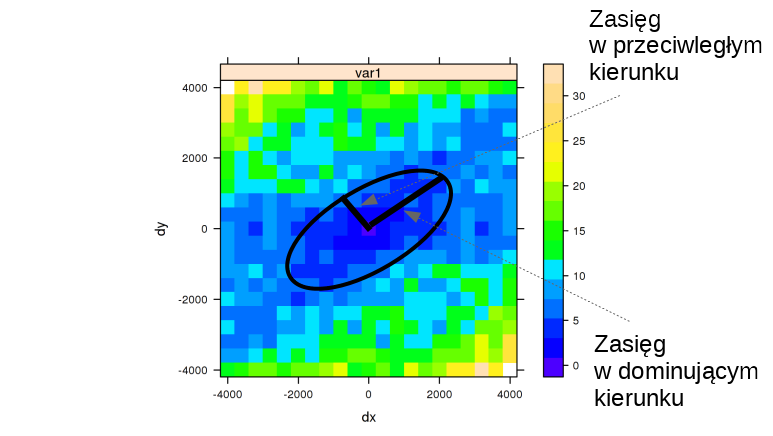
\includegraphics[width=1\linewidth]{figs/mapa_semiwariogramu} 

}

\caption{Podstawowe parametry mapy semiwariogramu.}\label{fig:07-modelowanie-33}
\end{figure}

W pakiecie \textbf{gstat} odbywa się to poprzez dodanie argumentu \texttt{alpha} do funkcji \texttt{variogram()}.
Należy w niej zdefiniować analizowane kierunki, które zostały określone na podstawie mapy semiwariogramu.
Następnie w funkcji \texttt{vgm()} należy podać nowy argument \texttt{anis}.
Przyjmuje on dwie wartości. Pierwsza z nich (\texttt{45} w przykładzie poniżej) oznacza dominujący kierunek anizotropii, druga zaś (\texttt{0.4}) mówi o tzw. proporcji anizotropii.
Proporcja anizotropii jest to relacja pomiędzy zmiennością na kierunku prostopadłym a głównym kierunku.
Na poniższym przykładzie zasięg ustalony dla głównego kierunku wynosi 4000 metrów.
Wartość proporcji anizotropii, \texttt{0.4}, w tym wypadku oznacza że dla prostopadłego kierunku zasięg będzie wynosił 1600 metrów (4000 metrów x 0.4) (rycina \ref{fig:07-modelowanie-34}).

\begin{Shaded}
\begin{Highlighting}[]
\NormalTok{vario\_map }\OtherTok{=} \FunctionTok{variogram}\NormalTok{(temp }\SpecialCharTok{\textasciitilde{}} \DecValTok{1}\NormalTok{, }
                      \AttributeTok{locations =}\NormalTok{ punkty,}
                      \AttributeTok{cutoff =} \DecValTok{4000}\NormalTok{,}
                      \AttributeTok{width =} \DecValTok{400}\NormalTok{, }
                      \AttributeTok{map =} \ConstantTok{TRUE}\NormalTok{)}
\FunctionTok{plot}\NormalTok{(vario\_map, }\AttributeTok{threshold =} \DecValTok{30}\NormalTok{, }
     \AttributeTok{col.regions =} \FunctionTok{hcl.colors}\NormalTok{(}\DecValTok{40}\NormalTok{, }\AttributeTok{palette =} \StringTok{"ag\_GrnYl"}\NormalTok{, }\AttributeTok{rev =} \ConstantTok{TRUE}\NormalTok{))}
\end{Highlighting}
\end{Shaded}

\begin{figure}

{\centering 
\includegraphics[width=1\linewidth]{07-modelowanie_files/figure-latex/07-modelowanie-34-1} 

}

\caption{Mapa semiwariogramu zmiennej temp.}\label{fig:07-modelowanie-34}
\end{figure}

Anizotropia może być także reprezentowana używając semiwariogramów kierunkowych (rycina \ref{fig:07-modelowanie-35})

\begin{Shaded}
\begin{Highlighting}[]
\NormalTok{vario\_kier }\OtherTok{=} \FunctionTok{variogram}\NormalTok{(temp }\SpecialCharTok{\textasciitilde{}} \DecValTok{1}\NormalTok{, }
                       \AttributeTok{locations =}\NormalTok{ punkty,}
                       \AttributeTok{alpha =} \FunctionTok{c}\NormalTok{(}\DecValTok{0}\NormalTok{, }\DecValTok{45}\NormalTok{, }\DecValTok{90}\NormalTok{, }\DecValTok{135}\NormalTok{),}
                       \AttributeTok{cutoff =} \DecValTok{4000}\NormalTok{)}
\FunctionTok{plot}\NormalTok{(vario\_kier)}
\end{Highlighting}
\end{Shaded}

\begin{figure}

{\centering 
\includegraphics[width=1\linewidth]{07-modelowanie_files/figure-latex/07-modelowanie-35-1} 

}

\caption{Semiwariogramy kierunkowe zmiennej temp.}\label{fig:07-modelowanie-35}
\end{figure}

Następnie semiwariogramy kierunkowe mogą być~modelowane ręcznie (rycina \ref{fig:07-modelowanie-36}) lub też używając automatycznego dopasowania (rycina \ref{fig:07-modelowanie-37}).

\begin{Shaded}
\begin{Highlighting}[]
\NormalTok{vario\_kier\_fit }\OtherTok{=} \FunctionTok{vgm}\NormalTok{(}\AttributeTok{psill =} \DecValTok{8}\NormalTok{, }\AttributeTok{model =} \StringTok{"Sph"}\NormalTok{, }\AttributeTok{range =} \DecValTok{4000}\NormalTok{, }
                     \AttributeTok{nugget =} \FloatTok{0.5}\NormalTok{, }\AttributeTok{anis =} \FunctionTok{c}\NormalTok{(}\DecValTok{45}\NormalTok{, }\FloatTok{0.4}\NormalTok{))}
\FunctionTok{plot}\NormalTok{(vario\_kier, vario\_kier\_fit, }\AttributeTok{as.table =} \ConstantTok{TRUE}\NormalTok{)}
\end{Highlighting}
\end{Shaded}

\begin{figure}

{\centering 
\includegraphics[width=1\linewidth]{07-modelowanie_files/figure-latex/07-modelowanie-36-1} 

}

\caption{Modele kierunkowe zmiennej temp.}\label{fig:07-modelowanie-36}
\end{figure}

\begin{Shaded}
\begin{Highlighting}[]
\NormalTok{vario\_kier\_fit2 }\OtherTok{=} \FunctionTok{fit.variogram}\NormalTok{(vario\_kier,}
                                \FunctionTok{vgm}\NormalTok{(}\AttributeTok{model =} \StringTok{"Sph"}\NormalTok{,}
                                    \AttributeTok{anis =} \FunctionTok{c}\NormalTok{(}\DecValTok{45}\NormalTok{, }\FloatTok{0.4}\NormalTok{), }
                                    \AttributeTok{nugget =} \FloatTok{0.5}\NormalTok{))}
\FunctionTok{plot}\NormalTok{(vario\_kier, vario\_kier\_fit2, }\AttributeTok{as.table =} \ConstantTok{TRUE}\NormalTok{)}
\end{Highlighting}
\end{Shaded}

\begin{figure}

{\centering 
\includegraphics[width=1\linewidth]{07-modelowanie_files/figure-latex/07-modelowanie-37-1} 

}

\caption{Automatycznie dopasowane modele kierunkowe zmiennej temp.}\label{fig:07-modelowanie-37}
\end{figure}

\section{Zadania}\label{z7}

Przyjrzyj się danym z obiektu \texttt{punkty\_pref}. Możesz go wczytać używając poniższego kodu:

\begin{Shaded}
\begin{Highlighting}[]
\FunctionTok{data}\NormalTok{(punkty\_pref)}
\end{Highlighting}
\end{Shaded}

\begin{enumerate}
\def\labelenumi{\arabic{enumi}.}
\tightlist
\item
  Zbuduj modele semiwariogramu zmiennej \texttt{srtm} używając modelu sferycznego używając zarówno ręcznie ustalonych parametrów oraz funkcji \texttt{fit.variogram()}.
  Porównaj graficznie uzyskane modele.
\item
  Zbuduj modele semiwariogramu zmiennej \texttt{srtm} używając modelu nuggetowego, sferycznego, wykładniczego, gausowskiego i potęgowego.
  Porównaj graficznie uzyskane modele.
\item
  Stwórz złożony model semiwariogramu zmiennej \texttt{srtm} używając modelu nuggetowego i sferycznego.
\item
  W oparciu o mapę semiwariogramu, zbuduj semiwariogramy kierunkowe zmiennej \texttt{srtm} dla kierunków wykazujących anizotropię przestrzenną.
  Następnie zbuduj modele semiwariogramu dla uzyskanych semiwariogramów kierunkowych.
\item
  (Dodatkowe) Spróbuj użyć jednego z modeli podstawowych, który nie był opisywany w tym rozdziale.
  Czym ten wybrany model się charakteryzuje?
\end{enumerate}

\chapter{Estymacje jednozmienne}\label{estymacje-jednozmienne}

Odtworzenie obliczeń z tego rozdziału wymaga załączenia poniższych pakietów oraz wczytania poniższych danych:

\begin{Shaded}
\begin{Highlighting}[]
\FunctionTok{library}\NormalTok{(sf)}
\FunctionTok{library}\NormalTok{(stars)}
\FunctionTok{library}\NormalTok{(gstat)}
\FunctionTok{library}\NormalTok{(tmap)}
\FunctionTok{library}\NormalTok{(geostatbook)}
\FunctionTok{data}\NormalTok{(punkty)}
\FunctionTok{data}\NormalTok{(siatka)}
\end{Highlighting}
\end{Shaded}

\section{Kriging}\label{kriging}

\subsection{Interpolacja geostatystyczna}\label{interpolacja-geostatystyczna}

Kriging (interpolacja geostatystyczna) to grupa metod estymacji zaproponowana w latach 50. przez Daniego Krige.
Główna zasada mówi, że prognoza w danej lokalizacji jest kombinacją obokległych obserwacji.
Waga nadawana każdej z obserwacji jest zależna od stopnia (przestrzennej) korelacji - stąd też bierze się istotna rola semiwariogramów.

\subsection{Metod krigingu}\label{metod-krigingu}

Istnieje szereg metod krigingu, w tym:

\begin{itemize}
\tightlist
\item
  Kriging prosty (ang. \emph{Simple kriging}) (sekcja \ref{kriging-prosty})
\item
  Kriging zwykły (ang. \emph{Ordinary kriging}) (sekcja \ref{kriging-zwykly})
\item
  Kriging z trendem (ang. \emph{Kriging with a trend}) (sekcja \ref{kriging-z-trendem})
\item
  Kriging stratyfikowany (ang. \emph{Kriging within strata} -- KWS)
\item
  Kriging prosty ze zmiennymi średnimi lokalnymi (ang. \emph{Simple kriging with varying local means} - SKlm) (sekcja \ref{SKlm})
\item
  Kriging z zewnętrznym trendem/Uniwersalny kriging (ang.\emph{Kriging with an external trend/Universal kriging}) (sekcja \ref{kriging-uniwersalny})
\item
  Kokriging (ang. \emph{Co-kriging}) (sekcja \ref{kokriging})
\item
  Kriging danych kodowanych (ang. \emph{Indicator kriging}) (sekcja \ref{kriging-danych-kodowanych})
\item
  Inne
\end{itemize}

\section{Kriging prosty}\label{kriging-prosty}

\subsection{\texorpdfstring{Kriging prosty (ang. \emph{Simple kriging})}{Kriging prosty (ang. Simple kriging)}}\label{kriging-prosty-ang.-simple-kriging}

Kriging prosty zakłada, że średnia jest znana i stała na całym obszarze.
W poniższym przykładzie po stworzeniu semiwariogramu empirycznego, dopasowano model semiwariogramu składający się z funkcji sferycznej o zasięgu 4000 metrów i wartości nuggetu równej 0,5 (rycina \ref{fig:08-estymacje-3}).

\begin{Shaded}
\begin{Highlighting}[]
\NormalTok{vario }\OtherTok{=} \FunctionTok{variogram}\NormalTok{(temp }\SpecialCharTok{\textasciitilde{}} \DecValTok{1}\NormalTok{, }\AttributeTok{locations =}\NormalTok{ punkty)}
\NormalTok{model }\OtherTok{=} \FunctionTok{vgm}\NormalTok{(}\DecValTok{10}\NormalTok{, }\AttributeTok{model =} \StringTok{"Sph"}\NormalTok{, }\AttributeTok{range =} \DecValTok{4000}\NormalTok{, }\AttributeTok{nugget =} \FloatTok{0.5}\NormalTok{)}
\NormalTok{model}
\end{Highlighting}
\end{Shaded}

\begin{verbatim}
##   model psill range
## 1   Nug   0.5     0
## 2   Sph  10.0  4000
\end{verbatim}

\begin{Shaded}
\begin{Highlighting}[]
\FunctionTok{plot}\NormalTok{(vario, }\AttributeTok{model =}\NormalTok{ model)}
\end{Highlighting}
\end{Shaded}

\begin{figure}

{\centering 
\includegraphics[width=1\linewidth]{08-estymacje_files/figure-latex/08-estymacje-3-1} 

}

\caption{Model złożony z modelu nuggetowego i sferycznego dla zmiennej temp.}\label{fig:08-estymacje-3}
\end{figure}

\begin{Shaded}
\begin{Highlighting}[]
\CommentTok{\# fitted = fit.variogram(vario, model)}
\end{Highlighting}
\end{Shaded}

Następnie następuje estymacja wartości z użyciem metody krigingu prostego.
W funkcji \texttt{krige()} z pakietu \textbf{gstat}, użycie tej metody wymaga ustalenia średniej wartości cechy za pomocą argumentu \texttt{beta}.

\begin{Shaded}
\begin{Highlighting}[]
\FunctionTok{mean}\NormalTok{(punkty}\SpecialCharTok{$}\NormalTok{temp)}
\end{Highlighting}
\end{Shaded}

\begin{verbatim}
## [1] 15.22251
\end{verbatim}

\begin{Shaded}
\begin{Highlighting}[]
\NormalTok{sk }\OtherTok{=} \FunctionTok{krige}\NormalTok{(temp }\SpecialCharTok{\textasciitilde{}} \DecValTok{1}\NormalTok{, }
            \AttributeTok{locations =}\NormalTok{ punkty,}
            \AttributeTok{newdata =}\NormalTok{ siatka,}
            \AttributeTok{model =}\NormalTok{ model,}
            \AttributeTok{beta =} \DecValTok{15}\NormalTok{)}
\end{Highlighting}
\end{Shaded}

\begin{verbatim}
## [using simple kriging]
\end{verbatim}

Wynik krigingu prostego, jak i każdy inny uzyskany z użyciem pakietu \textbf{gstat}, można podejrzeć wpisując nazwę wynikowego obiektu.
Szczególnie ważne są dwie, nowe zmienne - \texttt{var1.pred} oraz \texttt{var1.var}.
Pierwsza z nich oznacza wartość estymowaną dla każdego oczka siatki, druga zaś mówi o wariancji estymacji.

\begin{Shaded}
\begin{Highlighting}[]
\NormalTok{sk}
\end{Highlighting}
\end{Shaded}

\begin{verbatim}
## stars object with 2 dimensions and 2 attributes
## attribute(s):
##                Min.  1st Qu.    Median      Mean   3rd Qu.     Max. NA's
## var1.pred  8.473052 12.70587 14.961083 15.488215 17.711775 24.36355 1270
## var1.var   0.821095  1.61326  1.974793  2.041073  2.355011  6.26745 1270
## dimension(s):
##   from  to offset delta               refsys x/y
## x    1 127 745542    90 ETRS89 / Poland CS92 [x]
## y    1  96 721256   -90 ETRS89 / Poland CS92 [y]
\end{verbatim}

Obie uzyskane zmienne można wyświetlić z użyciem pakietu \textbf{tmap} (rycina \ref{fig:plotsy2}).

\begin{Shaded}
\begin{Highlighting}[]
\FunctionTok{tm\_shape}\NormalTok{(sk) }\SpecialCharTok{+}
        \FunctionTok{tm\_raster}\NormalTok{(}\AttributeTok{col =} \FunctionTok{c}\NormalTok{(}\StringTok{"var1.pred"}\NormalTok{, }\StringTok{"var1.var"}\NormalTok{),}
                  \AttributeTok{style =} \StringTok{"cont"}\NormalTok{, }
                  \AttributeTok{palette =} \FunctionTok{list}\NormalTok{(}\StringTok{"{-}Spectral"}\NormalTok{, }\StringTok{"viridis"}\NormalTok{)) }\SpecialCharTok{+}
        \FunctionTok{tm\_layout}\NormalTok{(}\AttributeTok{legend.frame =} \ConstantTok{TRUE}\NormalTok{)}
\end{Highlighting}
\end{Shaded}

\begin{figure}

{\centering 
\includegraphics[width=1\linewidth]{08-estymacje_files/figure-latex/plotsy2-1} 

}

\caption{Estymacja i wariancja estymacji używając metody krigingu prostego (SK).}\label{fig:plotsy2}
\end{figure}

\subsection{Kriging prosty po transformacji danych}\label{kriging-prosty-po-transformacji-danych}

Zarówno kriging prosty, jak i kolejne metody krigingowe opisane w tym skrypcie, mogą używać zmiennych wejściowych poddanych transformacjom, np. logaritmizacji (sekcja \ref{trans-danych}).
Może to mieć na celu zniwelowanie skośności rozkładu i w efekcie uzyskanie pewniejszych wyników.
Tutaj konieczne jest pamiętanie o kilku koniecznych krokach: (1) wykonaniu transformacji przy budowaniu semiwariogramu, (2) wykonaniu transformacji przy tworzeniu estymacji, oraz (3) zastosowaniu transformacji odwrotnej na uzyskanych wynikach.
Zobaczmy to na poniższym przykładzie.

W pierwszym etapie budujemy i modelujemy semiwariogram, jednakże zamiast używać bezpośrednio wartości zmiennej \texttt{temp} poddajemy ją logaritmizacji poprzez \texttt{log(temp)}.

\begin{Shaded}
\begin{Highlighting}[]
\NormalTok{vario\_kp2 }\OtherTok{=} \FunctionTok{variogram}\NormalTok{(}\FunctionTok{log}\NormalTok{(temp) }\SpecialCharTok{\textasciitilde{}} \DecValTok{1}\NormalTok{, }\AttributeTok{locations =}\NormalTok{ punkty)}
\NormalTok{model\_kp2 }\OtherTok{=} \FunctionTok{vgm}\NormalTok{(}\FloatTok{0.06}\NormalTok{, }\AttributeTok{model =} \StringTok{"Sph"}\NormalTok{, }\AttributeTok{range =} \DecValTok{4000}\NormalTok{, }\AttributeTok{nugget =} \FloatTok{0.002}\NormalTok{)}
\NormalTok{model\_kp2}
\end{Highlighting}
\end{Shaded}

\begin{verbatim}
##   model psill range
## 1   Nug 0.002     0
## 2   Sph 0.060  4000
\end{verbatim}

\begin{Shaded}
\begin{Highlighting}[]
\FunctionTok{plot}\NormalTok{(vario\_kp2, }\AttributeTok{model =}\NormalTok{ model\_kp2)}
\end{Highlighting}
\end{Shaded}

\begin{figure}

{\centering 
\includegraphics[width=1\linewidth]{08-estymacje_files/figure-latex/08-estymacje-3b-1} 

}

\caption{Model złożony z modelu nuggetowego i sferycznego dla zmiennej temp.}\label{fig:08-estymacje-3b}
\end{figure}

\begin{Shaded}
\begin{Highlighting}[]
\CommentTok{\# fitted\_kp2 = fit.variogram(vario\_kp2, model\_kp2)}
\end{Highlighting}
\end{Shaded}

Następnie, musimy określić logarytm średniej wartości badanej zmiennej dla całego obszaru oraz użyć logarytmu tej zmiennej do stworzenia estymacji.

\begin{Shaded}
\begin{Highlighting}[]
\FunctionTok{mean}\NormalTok{(}\FunctionTok{log}\NormalTok{(punkty}\SpecialCharTok{$}\NormalTok{temp))}
\end{Highlighting}
\end{Shaded}

\begin{verbatim}
## [1] 2.689027
\end{verbatim}

\begin{Shaded}
\begin{Highlighting}[]
\NormalTok{sk\_kp2 }\OtherTok{=} \FunctionTok{krige}\NormalTok{(}\FunctionTok{log}\NormalTok{(temp) }\SpecialCharTok{\textasciitilde{}} \DecValTok{1}\NormalTok{, }
            \AttributeTok{locations =}\NormalTok{ punkty,}
            \AttributeTok{newdata =}\NormalTok{ siatka,}
            \AttributeTok{model =}\NormalTok{ model\_kp2,}
            \AttributeTok{beta =} \FloatTok{2.69}\NormalTok{)}
\end{Highlighting}
\end{Shaded}

\begin{verbatim}
## [using simple kriging]
\end{verbatim}

Wynik krigingu prostego zawiera dwie zmienne - \texttt{var1.pred} oraz \texttt{var1.var}.
Co warte podkreślenia, pierwsza z nich określa wartość estymowaną dla każdego oczka siatki w logarytmie badanej jednostki.
Przykładowo, gdy nasza zmienna określała temperaturę~w stopniach Celsjusza, to wynik jest przestawiony w logarytmie stopni Celsjusza.

\begin{Shaded}
\begin{Highlighting}[]
\NormalTok{sk\_kp2}
\end{Highlighting}
\end{Shaded}

\begin{verbatim}
## stars object with 2 dimensions and 2 attributes
## attribute(s):
##                   Min.     1st Qu.     Median       Mean    3rd Qu.       Max.
## var1.pred  2.116458867 2.532130644 2.70146692 2.70654657 2.86844059 3.19736223
## var1.var   0.003507856 0.008334475 0.01053523 0.01092072 0.01284403 0.03625981
##            NA's
## var1.pred  1270
## var1.var   1270
## dimension(s):
##   from  to offset delta               refsys x/y
## x    1 127 745542    90 ETRS89 / Poland CS92 [x]
## y    1  96 721256   -90 ETRS89 / Poland CS92 [y]
\end{verbatim}

W związku z tym, koniecznym ostatnim krokiem jest przywrócenie oryginalnej jednostki.
Możemy to zrobić używając funkcji \texttt{rev\_trans()} z pakietu \textbf{geostatbook} (sekcja \ref{transformacja-odwrotna}), która przyjmuje naszą zlogaritmizowaną estymację, wariancję~estymacji i oryginalne wartości pomiarów w punktach.

\begin{Shaded}
\begin{Highlighting}[]
\NormalTok{sk\_kp2}\SpecialCharTok{$}\NormalTok{temp }\OtherTok{=} \FunctionTok{rev\_trans}\NormalTok{(sk\_kp2}\SpecialCharTok{$}\NormalTok{var1.pred, sk\_kp2}\SpecialCharTok{$}\NormalTok{var1.var, punkty}\SpecialCharTok{$}\NormalTok{temp)}
\NormalTok{sk\_kp2}
\end{Highlighting}
\end{Shaded}

\begin{verbatim}
## stars object with 2 dimensions and 3 attributes
## attribute(s):
##                   Min.      1st Qu.      Median        Mean     3rd Qu.
## var1.pred  2.116458867  2.532130644  2.70146692  2.70654657  2.86844059
## var1.var   0.003507856  0.008334475  0.01053523  0.01092072  0.01284403
## temp       8.187681121 12.430871960 14.72626722 15.22250747 17.40643717
##                   Max. NA's
## var1.pred   3.19736223 1270
## var1.var    0.03625981 1270
## temp       24.10950341 1270
## dimension(s):
##   from  to offset delta               refsys x/y
## x    1 127 745542    90 ETRS89 / Poland CS92 [x]
## y    1  96 721256   -90 ETRS89 / Poland CS92 [y]
\end{verbatim}

W efekcie otrzymujemy estymację w oryginalnych jednostkach - stopniach Celsjusza.
Trzy uzyskane zmienne można wyświetlić z użyciem pakietu \textbf{tmap} (rycina \ref{fig:plotsy2b}).

\begin{Shaded}
\begin{Highlighting}[]
\FunctionTok{tm\_shape}\NormalTok{(sk\_kp2) }\SpecialCharTok{+}
        \FunctionTok{tm\_raster}\NormalTok{(}\AttributeTok{col =} \FunctionTok{c}\NormalTok{(}\StringTok{"var1.pred"}\NormalTok{, }\StringTok{"var1.var"}\NormalTok{, }\StringTok{"temp"}\NormalTok{),}
                  \AttributeTok{style =} \StringTok{"cont"}\NormalTok{, }
                  \AttributeTok{palette =} \FunctionTok{list}\NormalTok{(}\StringTok{"{-}Spectral"}\NormalTok{, }\StringTok{"viridis"}\NormalTok{, }\StringTok{"{-}Spectral"}\NormalTok{)) }\SpecialCharTok{+}
        \FunctionTok{tm\_layout}\NormalTok{(}\AttributeTok{legend.frame =} \ConstantTok{TRUE}\NormalTok{)}
\end{Highlighting}
\end{Shaded}

\begin{figure}

{\centering 
\includegraphics[width=1\linewidth]{08-estymacje_files/figure-latex/plotsy2b-1} 

}

\caption{Estymacja logarytmu zmiennej temp, jej wariancja estymacji, oraz estymacja wartości tej zmiennej po przeprowadzeniu procesu transformacji odwrotnej.}\label{fig:plotsy2b}
\end{figure}

\section{Kriging zwykły}\label{kriging-zwykly}

\subsection{\texorpdfstring{Kriging zwykły (ang. \emph{Ordinary kriging})}{Kriging zwykły (ang. Ordinary kriging)}}\label{kriging-zwykux142y-ang.-ordinary-kriging}

W krigingu zwykłym średnia traktowana jest jako wartość nieznana.
Metoda ta uwzględnia lokalne fluktuacje średniej poprzez stosowanie ruchomego okna.
Parametry ruchomego okna można określić za pomocą jednego z dwóch argumentów:

\begin{itemize}
\tightlist
\item
  \texttt{nmax} - użyta zostanie określona liczba najbliższych obserwacji.
\item
  \texttt{maxdist} - użyte zostaną jedynie obserwacje w zadanej odległości.
\end{itemize}

\begin{Shaded}
\begin{Highlighting}[]
\CommentTok{\# ok = krige(temp \textasciitilde{} 1,}
\CommentTok{\#             locations = punkty,}
\CommentTok{\#             newdata = siatka, }
\CommentTok{\#             model = model, }
\CommentTok{\#             nmax = 30)}
\NormalTok{ok }\OtherTok{=} \FunctionTok{krige}\NormalTok{(temp }\SpecialCharTok{\textasciitilde{}} \DecValTok{1}\NormalTok{,}
            \AttributeTok{locations =}\NormalTok{ punkty,}
            \AttributeTok{newdata =}\NormalTok{ siatka, }
            \AttributeTok{model =}\NormalTok{ model, }
            \AttributeTok{maxdist =} \DecValTok{1500}\NormalTok{)}
\end{Highlighting}
\end{Shaded}

\begin{verbatim}
## [using ordinary kriging]
\end{verbatim}

Podobnie jak w przypadku krigingu prostego, można przyjrzeć się wynikom estymacji podając nazwę wynikowego obiektu oraz wyświetlić je używając funkcji \texttt{tm\_shape()} and \texttt{tm\_raster()} (rycina \ref{fig:plotsy2ok2}).

\begin{Shaded}
\begin{Highlighting}[]
\NormalTok{ok}
\end{Highlighting}
\end{Shaded}

\begin{verbatim}
## stars object with 2 dimensions and 2 attributes
## attribute(s):
##                 Min.  1st Qu.    Median      Mean  3rd Qu.      Max. NA's
## var1.pred  8.4763353 12.71717 14.967146 15.531098 17.70921 24.326622 1270
## var1.var   0.8215425  1.62057  1.990971  2.082008  2.39254  9.882173 1270
## dimension(s):
##   from  to offset delta               refsys x/y
## x    1 127 745542    90 ETRS89 / Poland CS92 [x]
## y    1  96 721256   -90 ETRS89 / Poland CS92 [y]
\end{verbatim}

\begin{Shaded}
\begin{Highlighting}[]
\FunctionTok{tm\_shape}\NormalTok{(ok) }\SpecialCharTok{+}
        \FunctionTok{tm\_raster}\NormalTok{(}\AttributeTok{col =} \FunctionTok{c}\NormalTok{(}\StringTok{"var1.pred"}\NormalTok{, }\StringTok{"var1.var"}\NormalTok{),}
                  \AttributeTok{style =} \StringTok{"cont"}\NormalTok{, }
                  \AttributeTok{palette =} \FunctionTok{list}\NormalTok{(}\StringTok{"{-}Spectral"}\NormalTok{, }\StringTok{"viridis"}\NormalTok{)) }\SpecialCharTok{+}
        \FunctionTok{tm\_layout}\NormalTok{(}\AttributeTok{legend.frame =} \ConstantTok{TRUE}\NormalTok{)}
\end{Highlighting}
\end{Shaded}

\begin{figure}

{\centering 
\includegraphics[width=1\linewidth]{08-estymacje_files/figure-latex/plotsy2ok2-1} 

}

\caption{Estymacja i wariancja estymacji używając metody krigingu zwykłego (OK).}\label{fig:plotsy2ok2}
\end{figure}

\section{Kriging z trendem}\label{kriging-z-trendem}

\subsection{\texorpdfstring{Kriging z trendem (ang. \emph{Kriging with a trend})}{Kriging z trendem (ang. Kriging with a trend)}}\label{kriging-z-trendem-ang.-kriging-with-a-trend}

Kriging z trendem, określany również jako kriging z wewnętrznym trendem, do estymacji wykorzystuje (oprócz zmienności wartości wraz z odległością) położenie analizowanych punktów.
W pierwszym kroku konieczne jest dodanie współrzędnych do używanego obiektu i do używanej siatki.

\begin{Shaded}
\begin{Highlighting}[]
\CommentTok{\# dodanie współrzędnych do punktów}
\NormalTok{punkty}\SpecialCharTok{$}\NormalTok{x }\OtherTok{=} \FunctionTok{st\_coordinates}\NormalTok{(punkty)[, }\DecValTok{1}\NormalTok{]}
\NormalTok{punkty}\SpecialCharTok{$}\NormalTok{y }\OtherTok{=} \FunctionTok{st\_coordinates}\NormalTok{(punkty)[, }\DecValTok{2}\NormalTok{]}
\CommentTok{\# dodanie współrzędnych do siatki}
\NormalTok{siatka}\SpecialCharTok{$}\NormalTok{x }\OtherTok{=} \FunctionTok{st\_coordinates}\NormalTok{(siatka)[, }\DecValTok{1}\NormalTok{]}
\NormalTok{siatka}\SpecialCharTok{$}\NormalTok{y }\OtherTok{=} \FunctionTok{st\_coordinates}\NormalTok{(siatka)[, }\DecValTok{2}\NormalTok{]}
\end{Highlighting}
\end{Shaded}

Współrzędne dodawane są do całej (regularnej) siatki.
Możemy przyciąć je do badanego obszaru poprzez wpisanie wartości \texttt{NA} w miejscach poza naszym obszarem zainteresowań.

\begin{Shaded}
\begin{Highlighting}[]
\NormalTok{siatka}\SpecialCharTok{$}\NormalTok{x[}\FunctionTok{is.na}\NormalTok{(siatka}\SpecialCharTok{$}\NormalTok{X2)] }\OtherTok{=} \ConstantTok{NA}
\NormalTok{siatka}\SpecialCharTok{$}\NormalTok{y[}\FunctionTok{is.na}\NormalTok{(siatka}\SpecialCharTok{$}\NormalTok{X2)] }\OtherTok{=} \ConstantTok{NA}
\end{Highlighting}
\end{Shaded}

Następnie pierwszy z argumentów w funkcji \texttt{variogram()} musi przyjąć postać \texttt{temp\ \textasciitilde{}\ x\ +\ y}, co oznacza, że uwzględniamy liniowy trend zależny od współrzędnej \texttt{x} oraz \texttt{y} (rycina \ref{fig:08-estymacje-11}).

\begin{Shaded}
\begin{Highlighting}[]
\NormalTok{vario\_kzt }\OtherTok{=} \FunctionTok{variogram}\NormalTok{(temp }\SpecialCharTok{\textasciitilde{}}\NormalTok{ x }\SpecialCharTok{+}\NormalTok{ y, }\AttributeTok{locations =}\NormalTok{ punkty)}
\FunctionTok{plot}\NormalTok{(vario\_kzt)}
\end{Highlighting}
\end{Shaded}

\begin{figure}

{\centering 
\includegraphics[width=1\linewidth]{08-estymacje_files/figure-latex/08-estymacje-11-1} 

}

\caption{Semiwariogram zmiennej temp uwzględniający współrzędne x i y.}\label{fig:08-estymacje-11}
\end{figure}

Dalszym etapem jest dopasowanie modelu semiwariancji, a następnie wyliczenie estymowanych wartości z użyciem funkcji \texttt{krige()}.
Należy tutaj pamiętać, aby wzór (w przykładzie \texttt{temp\ \textasciitilde{}\ x\ +\ y}) był taki sam podczas budowania semiwariogramu, jak i estymacji (rycina \ref{fig:08-estymacje-12}).

\begin{Shaded}
\begin{Highlighting}[]
\NormalTok{model\_kzt }\OtherTok{=} \FunctionTok{vgm}\NormalTok{(}\AttributeTok{model =} \StringTok{"Sph"}\NormalTok{, }\AttributeTok{nugget =} \DecValTok{1}\NormalTok{)}
\NormalTok{fitted\_kzt }\OtherTok{=} \FunctionTok{fit.variogram}\NormalTok{(vario\_kzt, model\_kzt)}
\NormalTok{fitted\_kzt}
\end{Highlighting}
\end{Shaded}

\begin{verbatim}
##   model     psill    range
## 1   Nug 0.2568762    0.000
## 2   Sph 6.7107464 2087.465
\end{verbatim}

\begin{Shaded}
\begin{Highlighting}[]
\FunctionTok{plot}\NormalTok{(vario\_kzt, fitted\_kzt)}
\end{Highlighting}
\end{Shaded}

\begin{figure}

{\centering 
\includegraphics[width=1\linewidth]{08-estymacje_files/figure-latex/08-estymacje-12-1} 

}

\caption{Model semiwariogramu zmiennej temp uwzględniający współrzędne x i y.}\label{fig:08-estymacje-12}
\end{figure}

\begin{Shaded}
\begin{Highlighting}[]
\NormalTok{kzt }\OtherTok{=} \FunctionTok{krige}\NormalTok{(temp }\SpecialCharTok{\textasciitilde{}}\NormalTok{ x }\SpecialCharTok{+}\NormalTok{ y, }
             \AttributeTok{locations =}\NormalTok{ punkty, }
             \AttributeTok{newdata =}\NormalTok{ siatka, }
             \AttributeTok{model =}\NormalTok{ fitted\_kzt)}
\end{Highlighting}
\end{Shaded}

\begin{verbatim}
## [using universal kriging]
\end{verbatim}

Wyświetlenie wyników odbywa się używając pakietu \textbf{tmap}.

\begin{Shaded}
\begin{Highlighting}[]
\FunctionTok{tm\_shape}\NormalTok{(kzt) }\SpecialCharTok{+}
        \FunctionTok{tm\_raster}\NormalTok{(}\AttributeTok{col =} \FunctionTok{c}\NormalTok{(}\StringTok{"var1.pred"}\NormalTok{, }\StringTok{"var1.var"}\NormalTok{),}
                  \AttributeTok{style =} \StringTok{"cont"}\NormalTok{, }
                  \AttributeTok{palette =} \FunctionTok{list}\NormalTok{(}\StringTok{"{-}Spectral"}\NormalTok{, }\StringTok{"viridis"}\NormalTok{)) }\SpecialCharTok{+}
        \FunctionTok{tm\_layout}\NormalTok{(}\AttributeTok{legend.frame =} \ConstantTok{TRUE}\NormalTok{)}
\end{Highlighting}
\end{Shaded}

\begin{figure}

{\centering 
\includegraphics[width=1\linewidth]{08-estymacje_files/figure-latex/plotsy2kzt-1} 

}

\caption{Estymacja i wariancja estymacji używając metody krigingu z trendem (KZT).}\label{fig:plotsy2kzt}
\end{figure}

\section{Porównanie wyników SK, SK (trans), OK i KZT}\label{poruxf3wnanie-wynikuxf3w-sk-sk-trans-ok-i-kzt}

Poniższe porównanie krigingu prostego (SK), krigingu prostego po zastosowaniu transformacji (SK trans), zwykłego (OK) i z trendem (KZT) wykazuje niewielkie różnice w uzyskanych wynikach (rycina \ref{fig:ploty-trzy}).

\begin{figure}

{\centering 
\includegraphics[width=1\linewidth]{08-estymacje_files/figure-latex/ploty-trzy-1} 

}

\caption{Porównanie wyników estymacji używając metody krigingu prostego (SK), krigingu zwykłego (OK) i krigingu z trendem (KZT).}\label{fig:ploty-trzy}
\end{figure}

W rozdziałach \ref{estymacje-wielozmienne} oraz \ref{wykorzystanie-do-estymacji-danych-uzupeniajacych} pokazane będą uzyskane wyniki interpolacji temperatury powietrza korzystając z innych metod krigingu.

\section{Zadania}\label{z8}

Zadania w tym rozdziale są oparte o dane z obiektu \texttt{punkty\_pref}.
Możesz go wczytać używając poniższego kodu:

\begin{Shaded}
\begin{Highlighting}[]
\FunctionTok{data}\NormalTok{(punkty\_pref)}
\end{Highlighting}
\end{Shaded}

Na jego podstawie stwórz trzy obiekty - \texttt{punkty\_pref1} zawierający wszystkie punkty, \texttt{punkty\_pref2} zawierający losowe 100 punktów, oraz \texttt{punkty\_pref3} zawierający losowe 30 punktów.

\begin{Shaded}
\begin{Highlighting}[]
\FunctionTok{set.seed}\NormalTok{(}\DecValTok{2018{-}11{-}25}\NormalTok{)}
\NormalTok{punkty\_pref1 }\OtherTok{=}\NormalTok{ punkty\_pref}
\NormalTok{punkty\_pref2 }\OtherTok{=}\NormalTok{ punkty\_pref[}\FunctionTok{sample}\NormalTok{(}\FunctionTok{nrow}\NormalTok{(punkty\_pref), }\DecValTok{100}\NormalTok{), ]}
\NormalTok{punkty\_pref3 }\OtherTok{=}\NormalTok{ punkty\_pref[}\FunctionTok{sample}\NormalTok{(}\FunctionTok{nrow}\NormalTok{(punkty\_pref), }\DecValTok{30}\NormalTok{), ]}
\end{Highlighting}
\end{Shaded}

\begin{enumerate}
\def\labelenumi{\arabic{enumi}.}
\tightlist
\item
  Zbuduj optymalne modele semiwariogramu zmiennej \texttt{srtm} dla trzech zbiorów danych - \texttt{punkty\_pref1}, \texttt{punkty\_pref2}, \texttt{punkty\_pref3}.
  Porównaj graficznie uzyskane modele.
\item
  W oparciu o uzyskane modele stwórz estymacje zmiennej \texttt{srtm} dla trzech zbiorów danych - \texttt{punkty\_pref1}, \texttt{punkty\_pref2}, \texttt{punkty\_pref3} używając krigingu prostego.
  Porównaj graficznie zarówno mapy estymacji jak i mapy wariancji.
  Opisz zaobserwowane różnice.
\item
  W oparciu o uzyskane modele stwórz estymacje zmiennej \texttt{srtm} dla zbioru danych \texttt{punkty\_pref3} używając krigingu zwykłego.
  Sprawdź jak wygląda wynik estymacji uwzględniając (i) 10 najbliższych obserwacji, (ii) 30 najbliższych obserwacji, (iii) obserwacje w odległości do 2 km.
\item
  Używając krigingu z trendem, stwórz optymalne modele zmiennej \texttt{srtm} dla dwóch zbiorów danych - \texttt{punkty\_pref1} oraz \texttt{punkty\_pref3}.
\item
  Porównaj graficznie zarówno mapy estymacji jak i mapy wariancji dla krigingu prostego, zwykłego oraz z trendem dla danych \texttt{punkty\_pref3}.
  Jakie można zauważyć podobieństwa a jakie różnice?
\item
  Dla zmiennej \texttt{temp} z obiektu \texttt{punkty\_pref1} stwórz mapę semiwariogramu.
  Czy ta zmienna wykazuje anizotropię przestrzenną?
  Jeżeli tak to stwórz semiwariogramy kierunkowe i ich modele, a następnie estymację zmiennej \texttt{temp}.
\end{enumerate}

\chapter{Estymacje używające danych uzupełniających}\label{wykorzystanie-do-estymacji-danych-uzupeniajacych}

Odtworzenie obliczeń z tego rozdziału wymaga załączenia poniższych pakietów oraz wczytania poniższych danych:

\begin{Shaded}
\begin{Highlighting}[]
\FunctionTok{library}\NormalTok{(sf)}
\FunctionTok{library}\NormalTok{(stars)}
\FunctionTok{library}\NormalTok{(gstat)}
\FunctionTok{library}\NormalTok{(tmap)}
\FunctionTok{library}\NormalTok{(geostatbook)}
\FunctionTok{data}\NormalTok{(punkty)}
\FunctionTok{data}\NormalTok{(siatka)}
\FunctionTok{data}\NormalTok{(dane\_uzup)}
\end{Highlighting}
\end{Shaded}

W wielu przypadkach, oprócz konkretnych pomiarów, istnieje również informacja na temat zmienności innych cech na analizowanym obszarze.
W sytuacji, gdy dodatkowe zmienne są skorelowane ze zmienną analizowaną można wykorzystać jedną z metod krigingu wykorzystującą dane uzupełniające, tj. kriging stratyfikowany, kriging prosty ze zmiennymi średnimi lokalnymi, czy kriging uniwersalny.

\begin{center}
\includegraphics[width=1\linewidth]{09-dane_uzupelniajace_files/figure-latex/09-dane-uzupelniajace-3-1} \end{center}

\section{Kriging prosty ze zmiennymi średnimi lokalnymi (LVM)}\label{SKlm}

\subsection{\texorpdfstring{Kriging prosty ze zmiennymi średnimi lokalnymi (LVM) (ang. \emph{Simple kriging with varying local means})}{Kriging prosty ze zmiennymi średnimi lokalnymi (LVM) (ang. Simple kriging with varying local means)}}\label{kriging-prosty-ze-zmiennymi-ux15brednimi-lokalnymi-lvm-ang.-simple-kriging-with-varying-local-means}

Kriging prosty ze zmiennymi średnimi lokalnymi zamiast znanej (stałej) stacjonarnej średniej wykorzystuje zmienne średnie lokalne uzyskane na podstawie innej informacji.

Lokalna średnia może być uzyskana za pomocą wyliczenia regresji liniowej pomiędzy zmienną badaną a zmienną dodatkową.
W takiej sytuacji konieczne jest użycie funkcji \texttt{lm()}.
W poniższym przykładzie budowany jest model liniowy relacji pomiędzy temperaturą powietrza (\texttt{temp}), a wysokością nad poziomem morza (\texttt{srtm}).

\begin{Shaded}
\begin{Highlighting}[]
\NormalTok{coef }\OtherTok{=} \FunctionTok{lm}\NormalTok{(temp }\SpecialCharTok{\textasciitilde{}}\NormalTok{ srtm, punkty)}\SpecialCharTok{$}\NormalTok{coef}
\NormalTok{coef}
\end{Highlighting}
\end{Shaded}

\begin{verbatim}
## (Intercept)        srtm 
## 17.41296753 -0.01021971
\end{verbatim}

Wykorzystując relację pomiędzy tymi dwoma zmiennymi tworzony jest semiwariogram empiryczny, który następnie jest modelowany (rycina \ref{fig:09-dane-uzupelniajace-5}).

\begin{Shaded}
\begin{Highlighting}[]
\NormalTok{vario }\OtherTok{=} \FunctionTok{variogram}\NormalTok{(temp }\SpecialCharTok{\textasciitilde{}}\NormalTok{ srtm, }\AttributeTok{location =}\NormalTok{ punkty)}
\NormalTok{model\_sim }\OtherTok{=} \FunctionTok{vgm}\NormalTok{(}\AttributeTok{model =} \StringTok{"Sph"}\NormalTok{, }\AttributeTok{nugget =} \DecValTok{1}\NormalTok{)}
\NormalTok{fitted\_sim }\OtherTok{=} \FunctionTok{fit.variogram}\NormalTok{(vario, model\_sim)}
\NormalTok{fitted\_sim}
\end{Highlighting}
\end{Shaded}

\begin{verbatim}
##   model      psill    range
## 1   Nug  0.6756367    0.000
## 2   Sph 13.1450299 5085.204
\end{verbatim}

\begin{Shaded}
\begin{Highlighting}[]
\FunctionTok{plot}\NormalTok{(vario, }\AttributeTok{model =}\NormalTok{ fitted\_sim)}
\end{Highlighting}
\end{Shaded}

\begin{figure}

{\centering 
\includegraphics[width=1\linewidth]{09-dane_uzupelniajace_files/figure-latex/09-dane-uzupelniajace-5-1} 

}

\caption{Model semiwariogramu zmiennej temp używając zmiennej srtm.}\label{fig:09-dane-uzupelniajace-5}
\end{figure}

Ostatnim krokiem jest estymacja geostatystyczna, w której oprócz czterech podstawowych argumentów, definiujemy także parametr \texttt{beta}.
W tym wypadku jest to wypadku obiekt uzyskany na podstawie regresji liniowej.

\begin{Shaded}
\begin{Highlighting}[]
\NormalTok{sk\_lvm }\OtherTok{=} \FunctionTok{krige}\NormalTok{(temp }\SpecialCharTok{\textasciitilde{}}\NormalTok{ srtm, }
               \AttributeTok{location =}\NormalTok{ punkty, }
               \AttributeTok{newdata =}\NormalTok{ dane\_uzup, }
               \AttributeTok{model =}\NormalTok{ fitted\_sim, }
               \AttributeTok{beta =}\NormalTok{ coef)}
\end{Highlighting}
\end{Shaded}

\begin{verbatim}
## [using simple kriging]
\end{verbatim}

\begin{Shaded}
\begin{Highlighting}[]
\NormalTok{sk\_lvm}
\end{Highlighting}
\end{Shaded}

\begin{verbatim}
## stars object with 2 dimensions and 2 attributes
## attribute(s):
##                Min.   1st Qu.    Median      Mean   3rd Qu.      Max. NA's
## var1.pred  8.559515 12.745494 14.958937 15.523648 17.759209 24.240945 1242
## var1.var   1.066204  1.875899  2.248138  2.321278  2.638222  6.852509 1242
## dimension(s):
##   from  to offset delta               refsys x/y
## x    1 127 745542    90 ETRS89 / Poland CS92 [x]
## y    1  96 721256   -90 ETRS89 / Poland CS92 [y]
\end{verbatim}

\begin{Shaded}
\begin{Highlighting}[]
\FunctionTok{tm\_shape}\NormalTok{(sk\_lvm) }\SpecialCharTok{+}
        \FunctionTok{tm\_raster}\NormalTok{(}\AttributeTok{col =} \FunctionTok{c}\NormalTok{(}\StringTok{"var1.pred"}\NormalTok{, }\StringTok{"var1.var"}\NormalTok{),}
                  \AttributeTok{style =} \StringTok{"cont"}\NormalTok{, }
                  \AttributeTok{palette =} \FunctionTok{list}\NormalTok{(}\StringTok{"{-}Spectral"}\NormalTok{, }\StringTok{"viridis"}\NormalTok{)) }\SpecialCharTok{+}
        \FunctionTok{tm\_layout}\NormalTok{(}\AttributeTok{legend.frame =} \ConstantTok{TRUE}\NormalTok{)}
\end{Highlighting}
\end{Shaded}

\begin{figure}

{\centering 
\includegraphics[width=1\linewidth]{09-dane_uzupelniajace_files/figure-latex/plotsylvm2-1} 

}

\caption{Estymacja i wariancja estymacji używając metody prostego krigingu ze zmiennymi średnimi lokalnymi (LVM).}\label{fig:plotsylvm2}
\end{figure}

\section{Kriging uniwersalny}\label{kriging-uniwersalny}

\subsection{\texorpdfstring{Kriging uniwersalny (ang. \emph{Universal kriging})}{Kriging uniwersalny (ang. Universal kriging)}}\label{kriging-uniwersalny-ang.-universal-kriging}

Kriging uniwersalny, określany również jako kriging z trendem (ang. \emph{Kriging with a trend model}) zakłada, że nieznana średnia lokalna zmienia się stopniowo na badanym obszarze.
W krigingu uniwersalnym możemy stosować zarówno zmienne jakościowe, jak i ilościowe.

W pierwszym przykładzie, kriging uniwersalny służy stworzeniu semiwariogramu, modelowaniu oraz estymacji temperatury powietrza z użyciem zmiennej pokrycia terenu (ryciny \ref{fig:09-dane-uzupelniajace-7}, \ref{fig:09-dane-uzupelniajace-8}, \ref{fig:plotsy4uk1}).

\begin{Shaded}
\begin{Highlighting}[]
\NormalTok{punkty}\SpecialCharTok{$}\NormalTok{clc }\OtherTok{=} \FunctionTok{as.factor}\NormalTok{(punkty}\SpecialCharTok{$}\NormalTok{clc)}
\NormalTok{vario\_uk1 }\OtherTok{=} \FunctionTok{variogram}\NormalTok{(temp }\SpecialCharTok{\textasciitilde{}}\NormalTok{ clc, }\AttributeTok{location =}\NormalTok{ punkty)}
\CommentTok{\# vario\_uk1}
\CommentTok{\# plot(vario\_uk1)}
\NormalTok{model\_uk1 }\OtherTok{=} \FunctionTok{vgm}\NormalTok{(}\AttributeTok{model =} \StringTok{"Sph"}\NormalTok{, }\AttributeTok{nugget =} \DecValTok{1}\NormalTok{)}
\NormalTok{vario\_fit\_uk1 }\OtherTok{=} \FunctionTok{fit.variogram}\NormalTok{(vario\_uk1, }\AttributeTok{model =}\NormalTok{ model\_uk1)}
\NormalTok{vario\_fit\_uk1}
\end{Highlighting}
\end{Shaded}

\begin{verbatim}
##   model    psill    range
## 1   Nug 1.626245    0.000
## 2   Sph 9.059005 6426.143
\end{verbatim}

\begin{Shaded}
\begin{Highlighting}[]
\FunctionTok{plot}\NormalTok{(vario\_uk1, vario\_fit\_uk1)}
\end{Highlighting}
\end{Shaded}

\begin{figure}

{\centering 
\includegraphics[width=1\linewidth]{09-dane_uzupelniajace_files/figure-latex/09-dane-uzupelniajace-7-1} 

}

\caption{Model semiwariogramu zmiennej temp używając zmiennej clc.}\label{fig:09-dane-uzupelniajace-7}
\end{figure}

\begin{Shaded}
\begin{Highlighting}[]
\NormalTok{dane\_uzup}\SpecialCharTok{$}\NormalTok{clc }\OtherTok{=} \FunctionTok{as.factor}\NormalTok{(dane\_uzup}\SpecialCharTok{$}\NormalTok{clc)}
\FunctionTok{tm\_shape}\NormalTok{(dane\_uzup[}\StringTok{"clc"}\NormalTok{]) }\SpecialCharTok{+}
        \FunctionTok{tm\_raster}\NormalTok{(}\AttributeTok{palette =} \FunctionTok{c}\NormalTok{(}\StringTok{"\#d9d40c"}\NormalTok{, }\StringTok{"\#416422"}\NormalTok{, }\StringTok{"\#0c6cae"}\NormalTok{))}
\end{Highlighting}
\end{Shaded}

\begin{figure}

{\centering 
\includegraphics[width=1\linewidth]{09-dane_uzupelniajace_files/figure-latex/09-dane-uzupelniajace-8-1} 

}

\caption{Rozkład przestrzenny wartości zmiennej clc używanej w modelu.}\label{fig:09-dane-uzupelniajace-8}
\end{figure}

\begin{Shaded}
\begin{Highlighting}[]
\NormalTok{uk1 }\OtherTok{=} \FunctionTok{krige}\NormalTok{(temp }\SpecialCharTok{\textasciitilde{}}\NormalTok{ clc, }
            \AttributeTok{locations =}\NormalTok{ punkty,}
            \AttributeTok{newdata =}\NormalTok{ dane\_uzup, }
            \AttributeTok{model =}\NormalTok{ vario\_fit\_uk1)}
\end{Highlighting}
\end{Shaded}

\begin{verbatim}
## [using universal kriging]
\end{verbatim}

\begin{Shaded}
\begin{Highlighting}[]
\FunctionTok{tm\_shape}\NormalTok{(uk1) }\SpecialCharTok{+}
        \FunctionTok{tm\_raster}\NormalTok{(}\AttributeTok{col =} \FunctionTok{c}\NormalTok{(}\StringTok{"var1.pred"}\NormalTok{, }\StringTok{"var1.var"}\NormalTok{),}
                  \AttributeTok{style =} \StringTok{"cont"}\NormalTok{, }
                  \AttributeTok{palette =} \FunctionTok{list}\NormalTok{(}\StringTok{"{-}Spectral"}\NormalTok{, }\StringTok{"viridis"}\NormalTok{)) }\SpecialCharTok{+}
        \FunctionTok{tm\_layout}\NormalTok{(}\AttributeTok{legend.frame =} \ConstantTok{TRUE}\NormalTok{)}
\end{Highlighting}
\end{Shaded}

\begin{figure}

{\centering 
\includegraphics[width=1\linewidth]{09-dane_uzupelniajace_files/figure-latex/plotsy4uk1-1} 

}

\caption{Estymacja i wariancja estymacji używając zmiennej clc i metody krigingu uniwersalnego (KU).}\label{fig:plotsy4uk1}
\end{figure}

W kolejnym przykładzie zastosowane są już dwie zmienne uzupełniające - wartość wskaźnika wegetacji (\texttt{ndvi}) oraz wysokość nad poziomem morza (\texttt{srtm}) (ryciny \ref{fig:09-dane-uzupelniajace-10}, \ref{fig:plotsy4KU}).

\begin{Shaded}
\begin{Highlighting}[]
\NormalTok{vario\_uk2 }\OtherTok{=} \FunctionTok{variogram}\NormalTok{(temp }\SpecialCharTok{\textasciitilde{}}\NormalTok{ ndvi }\SpecialCharTok{+}\NormalTok{ srtm, }\AttributeTok{location =}\NormalTok{ punkty)}
\CommentTok{\# vario\_uk2}
\CommentTok{\# plot(vario\_uk2)}
\NormalTok{model }\OtherTok{=} \FunctionTok{vgm}\NormalTok{(}\AttributeTok{model =} \StringTok{"Sph"}\NormalTok{, }\AttributeTok{nugget =} \DecValTok{1}\NormalTok{)}
\NormalTok{vario\_fit\_uk2 }\OtherTok{=} \FunctionTok{fit.variogram}\NormalTok{(vario\_uk2, }\AttributeTok{model =}\NormalTok{ model)}
\NormalTok{vario\_fit\_uk2}
\end{Highlighting}
\end{Shaded}

\begin{verbatim}
##   model      psill    range
## 1   Nug  0.7602125    0.000
## 2   Sph 12.4326154 5188.676
\end{verbatim}

\begin{Shaded}
\begin{Highlighting}[]
\FunctionTok{plot}\NormalTok{(vario\_uk2, vario\_fit\_uk2)}
\end{Highlighting}
\end{Shaded}

\begin{figure}

{\centering 
\includegraphics[width=1\linewidth]{09-dane_uzupelniajace_files/figure-latex/09-dane-uzupelniajace-10-1} 

}

\caption{Model semiwariogramu zmiennej temp używając zmiennych ndvi i srtm.}\label{fig:09-dane-uzupelniajace-10}
\end{figure}

\begin{Shaded}
\begin{Highlighting}[]
\NormalTok{uk2 }\OtherTok{=} \FunctionTok{krige}\NormalTok{(temp }\SpecialCharTok{\textasciitilde{}}\NormalTok{ ndvi }\SpecialCharTok{+}\NormalTok{ srtm,}
             \AttributeTok{locations =}\NormalTok{ punkty, }
             \AttributeTok{newdata =}\NormalTok{ dane\_uzup,}
             \AttributeTok{model =}\NormalTok{ vario\_fit\_uk2)}
\end{Highlighting}
\end{Shaded}

\begin{verbatim}
## [using universal kriging]
\end{verbatim}

\begin{Shaded}
\begin{Highlighting}[]
\FunctionTok{tm\_shape}\NormalTok{(uk2) }\SpecialCharTok{+}
        \FunctionTok{tm\_raster}\NormalTok{(}\AttributeTok{col =} \FunctionTok{c}\NormalTok{(}\StringTok{"var1.pred"}\NormalTok{, }\StringTok{"var1.var"}\NormalTok{),}
                  \AttributeTok{style =} \StringTok{"cont"}\NormalTok{, }
                  \AttributeTok{palette =} \FunctionTok{list}\NormalTok{(}\StringTok{"{-}Spectral"}\NormalTok{, }\StringTok{"viridis"}\NormalTok{)) }\SpecialCharTok{+}
        \FunctionTok{tm\_layout}\NormalTok{(}\AttributeTok{legend.frame =} \ConstantTok{TRUE}\NormalTok{)}
\end{Highlighting}
\end{Shaded}

\begin{figure}

{\centering 
\includegraphics[width=1\linewidth]{09-dane_uzupelniajace_files/figure-latex/plotsy4KU-1} 

}

\caption{Estymacja i wariancja estymacji używając zmiennych ndvi i srtm i metody krigingu uniwersalnego (KU).}\label{fig:plotsy4KU}
\end{figure}

\section{Zadania}\label{z11}

Zadania w tym rozdziale są oparte o dane z obiektu \texttt{punkty}.

\begin{Shaded}
\begin{Highlighting}[]
\FunctionTok{data}\NormalTok{(punkty)}
\end{Highlighting}
\end{Shaded}

\begin{enumerate}
\def\labelenumi{\arabic{enumi}.}
\tightlist
\item
  Zastosuj kriging prosty ze zmiennymi średnimi lokalnymi do stworzenia estymacji zmiennej \texttt{ndvi} używając jej relacji ze zmienną \texttt{savi}.
\item
  Stwórz estymację krigingu uniwersalnego dla zmiennej \texttt{ndvi} używając jej relacji ze zmienną \texttt{savi}.
\item
  Stwórz estymację krigingu uniwersalnego dla zmiennej \texttt{ndvi} używając jej relacji ze zmiennymi \texttt{clc}, \texttt{srtm}, \texttt{temp} i \texttt{savi}.
\item
  Porównaj graficznie trzy powyższe estymacje.
  Opisz podobieństwa i różnice.
\end{enumerate}

\chapter{Estymacje wielozmienne}\label{estymacje-wielozmienne}

Odtworzenie obliczeń z tego rozdziału wymaga załączenia poniższych pakietów oraz wczytania poniższych danych:

\begin{Shaded}
\begin{Highlighting}[]
\FunctionTok{library}\NormalTok{(sf)}
\FunctionTok{library}\NormalTok{(stars)}
\FunctionTok{library}\NormalTok{(gstat)}
\FunctionTok{library}\NormalTok{(tmap)}
\FunctionTok{library}\NormalTok{(geostatbook)}
\FunctionTok{data}\NormalTok{(punkty)}
\FunctionTok{data}\NormalTok{(punkty\_ndvi)}
\FunctionTok{data}\NormalTok{(siatka)}
\end{Highlighting}
\end{Shaded}

\section{Kokriging}\label{kokriging}

\subsection{\texorpdfstring{Kokriging (ang. \emph{co-kriging})}{Kokriging (ang. co-kriging)}}\label{kokriging-ang.-co-kriging}

Kokriging pozwala na wykorzystanie dodatkowej zmiennej (ang. \emph{auxiliary variable}), zwanej inaczej kozmienną (ang. \emph{co-variable}), która może być użyta do prognozowania wartości badanej zmiennej w nieopróbowanej lokalizacji.
Zmienna dodatkowa może być pomierzona w tych samych miejscach, gdzie badana zmienna, jak też w innych niż badana zmienna.
Możliwa jest też sytuacja, gdy zmienna dodatkowa jest pomierzona w dwóch powyższych przypadkach.
Kokriging wymaga, aby obie zmienne były istotnie ze sobą skorelowane.
Najczęściej kokriging jest stosowany w sytuacji, gdy zmienna dodatkowa jest łatwiejsza (tańsza) do pomierzenia niż zmienna główna.
W efekcie, uzyskany zbiór danych zawiera informacje o badanej zmiennej oraz gęściej opróbowane informacje o zmiennej dodatkowej.
Jeżeli informacje o zmiennej dodatkowej są znane dla całego obszaru wówczas bardziej odpowiednią techniką będzie kriging z zewnętrznym trendem (KED).

\subsection{Wybór dodatkowej zmiennej}\label{wybuxf3r-dodatkowej-zmiennej}

Wybór zmiennej dodatkowej może opierać się na dwóch kryteriach:

\begin{itemize}
\tightlist
\item
  Teoretycznym
\item
  Empirycznym
\end{itemize}

\section{Krossemiwariogramy}\label{krossemiwariogramy}

\subsection{\texorpdfstring{Krossemiwariogramy (ang. \textbf{crossvariogram})}{Krossemiwariogramy (ang. crossvariogram)}}\label{krossemiwariogramy-ang.-crossvariogram}

Metoda kokrigingu opiera się nie o semiwariogram, lecz o krossemiwariogramy.
Krossemiwariogram jest to wariancja różnicy pomiędzy dwiema zmiennymi w dwóch lokalizacjach.
Wyliczając krossemiwariogram otrzymujemy empiryczne semiwariogramy dla dwóch badanych zmiennych oraz krosswariogram dla kombinacji dwóch zmiennych.

W poniższym przykładzie istnieją dwie zmienne, \texttt{savi} ze zbioru \texttt{punkty} pomierzona w 242 lokalizacjach oraz \texttt{ndvi} ze zbioru \texttt{punkty\_ndvi} pomierzona w 992 punktach (ryciny \ref{fig:10-kokriging-3} i \ref{fig:10-kokriging-3}).

\begin{Shaded}
\begin{Highlighting}[]
\FunctionTok{tm\_shape}\NormalTok{(punkty) }\SpecialCharTok{+}
        \FunctionTok{tm\_symbols}\NormalTok{(}\AttributeTok{col =} \StringTok{"savi"}\NormalTok{)}
\end{Highlighting}
\end{Shaded}

\begin{figure}

{\centering 
\includegraphics[width=1\linewidth]{10-kokriging_files/figure-latex/10-kokriging-3-1} 

}

\caption{Mapa wartości zmiennej savi.}\label{fig:10-kokriging-3}
\end{figure}

\begin{Shaded}
\begin{Highlighting}[]
\FunctionTok{tm\_shape}\NormalTok{(punkty\_ndvi) }\SpecialCharTok{+}
        \FunctionTok{tm\_symbols}\NormalTok{(}\AttributeTok{col =} \StringTok{"ndvi"}\NormalTok{)}
\end{Highlighting}
\end{Shaded}

\begin{figure}

{\centering 
\includegraphics[width=1\linewidth]{10-kokriging_files/figure-latex/10-kokriging-4-1} 

}

\caption{Mapa wartości zmiennej ndvi.}\label{fig:10-kokriging-4}
\end{figure}

Tworzenie krossemiwariogramów odbywa się z użyciem funkcji \texttt{gstat()}. Na początku definiujemy pierwszy obiekt \texttt{g}.
Składa się on z obiektu pustego (\texttt{NULL}), nazwy pierwszej zmiennej (nazwa może być dowolna), wzoru (w przykładzie \texttt{savi\ \textasciitilde{}\ 1}), oraz pierwszego zbioru punktowego.
Następnie do pierwszego obiektu \texttt{g} dodajemy nowe informacje również poprzez funkcję \texttt{gstat()}. Jest to nazwa obiektu (\texttt{g}), nazwa drugiej zmiennej, wzór, oraz drugi zbiór punktowy.

\begin{Shaded}
\begin{Highlighting}[]
\NormalTok{g }\OtherTok{=} \FunctionTok{gstat}\NormalTok{(}\ConstantTok{NULL}\NormalTok{, }
          \AttributeTok{id =} \StringTok{"SAVI"}\NormalTok{, }
          \AttributeTok{form =}\NormalTok{ savi }\SpecialCharTok{\textasciitilde{}} \DecValTok{1}\NormalTok{, }
          \AttributeTok{data =}\NormalTok{ punkty)}
\NormalTok{g }\OtherTok{=} \FunctionTok{gstat}\NormalTok{(g, }
          \AttributeTok{id =} \StringTok{"NDVI"}\NormalTok{, }
          \AttributeTok{form =}\NormalTok{ ndvi }\SpecialCharTok{\textasciitilde{}} \DecValTok{1}\NormalTok{, }
          \AttributeTok{data =}\NormalTok{ punkty\_ndvi)}
\NormalTok{g}
\end{Highlighting}
\end{Shaded}

\begin{verbatim}
## data:
## SAVI : formula = savi`~`1 ; data dim = 242 x 5
## NDVI : formula = ndvi`~`1 ; data dim = 992 x 1
\end{verbatim}

Z uzyskanego w ten sposób obiektu tworzymy krossemiwariogram (funkcja \texttt{variogram()}), a następnie go wizualizujemy używając funkcji \texttt{plot()} (rycina \ref{fig:10-kokriging-6}).

\begin{Shaded}
\begin{Highlighting}[]
\NormalTok{v }\OtherTok{=} \FunctionTok{variogram}\NormalTok{(g)}
\FunctionTok{plot}\NormalTok{(v)}
\end{Highlighting}
\end{Shaded}

\begin{figure}

{\centering 
\includegraphics[width=1\linewidth]{10-kokriging_files/figure-latex/10-kokriging-6-1} 

}

\caption{Krossemiwariogram zmiennych savi i ndvi.}\label{fig:10-kokriging-6}
\end{figure}

\section{Modelowanie krossemiwariogramów}\label{modelowanie-krossemiwariogramuxf3w}

Modelowanie krossemiwariogramów, podobnie jak ich tworzenie, odbywa się używając funkcji \texttt{gstat()},
gdzie podaje się wcześniejszy obiekt \texttt{g}, model, oraz argument \texttt{fill.all\ =\ TRUE}.
Ten ostatni parametr powoduje, że model dodawany jest do wszystkich elementów krossemiwariogramu.

\begin{Shaded}
\begin{Highlighting}[]
\NormalTok{g\_model }\OtherTok{=} \FunctionTok{vgm}\NormalTok{(}\FloatTok{0.006}\NormalTok{, }\AttributeTok{model =} \StringTok{"Sph"}\NormalTok{,}
              \AttributeTok{range =} \DecValTok{1200}\NormalTok{, }\AttributeTok{nugget =} \FloatTok{0.001}\NormalTok{)}
\NormalTok{g1 }\OtherTok{=} \FunctionTok{gstat}\NormalTok{(g, }\AttributeTok{model =}\NormalTok{ g\_model, }\AttributeTok{fill.all =} \ConstantTok{TRUE}\NormalTok{)}
\NormalTok{g1}
\end{Highlighting}
\end{Shaded}

\begin{verbatim}
## data:
## SAVI : formula = savi`~`1 ; data dim = 242 x 5
## NDVI : formula = ndvi`~`1 ; data dim = 992 x 1
## variograms:
##              model psill range
## SAVI[1]        Nug 0.001     0
## SAVI[2]        Sph 0.006  1200
## NDVI[1]        Nug 0.001     0
## NDVI[2]        Sph 0.006  1200
## SAVI.NDVI[1]   Nug 0.001     0
## SAVI.NDVI[2]   Sph 0.006  1200
\end{verbatim}

W przypadku semiwariogramów funkcja \texttt{fit.variogram()} służyła dopasowaniu parametrów modelu do semiwariogramu empirycznego.
Podobną rolę w krossemiwariogramach spełnia funkcja \texttt{fit.lmc()} - dopasowuje ona liniowy model koregionalizacji do semiwariogramów wielozmienych (rycina \ref{fig:10-kokriging-8}).
Funkcja \texttt{fit.lmc()} oczekuje co najmniej dwóch elementów, krossemiwariogramu oraz modelów krossemiwariancji.
W poniższym przykładzie dodatkowo użyto parametru \texttt{correct.diagonal\ =\ 1.01}, z uwagi na to że analizowane zmienne wykazywały bardzo silną korelację oraz parametru \texttt{fit.method}.
Ten ostatni parametr określa, która z użytych metod automatycznego dopasowania semiwariogramów jest używana.
Pakiet \textbf{gstat} ma domyślnie ustawione \texttt{fit.method\ =\ 7}, co daje największe znaczenie parom punktów o najmniejszym zasięgu.
Ta opcja nie jest zazwyczaj optymalna w przypadku krossemiwariogramów - tutaj częściej stosuje się \texttt{fit.method\ =\ 6} (wagi nie są nadawane) lub \texttt{fit.method\ =\ 1} (wagi proporcjonalne do liczby par punktów w każdym przedziale).

\begin{Shaded}
\begin{Highlighting}[]
\NormalTok{g2 }\OtherTok{=} \FunctionTok{fit.lmc}\NormalTok{(v, g1,}
                \AttributeTok{correct.diagonal =} \FloatTok{1.01}\NormalTok{,}
                \AttributeTok{fit.method =} \DecValTok{6}\NormalTok{)}
\NormalTok{g2}
\end{Highlighting}
\end{Shaded}

\begin{verbatim}
## data:
## SAVI : formula = savi`~`1 ; data dim = 242 x 5
## NDVI : formula = ndvi`~`1 ; data dim = 992 x 1
## variograms:
##              model        psill range
## SAVI[1]        Nug 0.0009873135     0
## SAVI[2]        Sph 0.0050465345  1200
## NDVI[1]        Nug 0.0023006100     0
## NDVI[2]        Sph 0.0070299532  1200
## SAVI.NDVI[1]   Nug 0.0014922022     0
## SAVI.NDVI[2]   Sph 0.0055018027  1200
\end{verbatim}

\begin{Shaded}
\begin{Highlighting}[]
\FunctionTok{plot}\NormalTok{(v, g2)}
\end{Highlighting}
\end{Shaded}

\begin{figure}

{\centering 
\includegraphics[width=1\linewidth]{10-kokriging_files/figure-latex/10-kokriging-8-1} 

}

\caption{Automatycznie dopasowane modele krossemiwariogramu zmiennych savi i ndvi.}\label{fig:10-kokriging-8}
\end{figure}

\section{Kokriging}\label{kokriging-1}

Posiadając dopasowane modele oraz siatkę można uzyskać wynik używając funkcji \texttt{predict()} (rycina \ref{fig:kokriging-predicted}).

\begin{Shaded}
\begin{Highlighting}[]
\NormalTok{ck }\OtherTok{=} \FunctionTok{predict}\NormalTok{(g2, }\AttributeTok{newdata =}\NormalTok{ siatka)}
\end{Highlighting}
\end{Shaded}

\begin{verbatim}
## Linear Model of Coregionalization found. Good.
## [using ordinary cokriging]
\end{verbatim}

W efekcie otrzymujemy pięć zmiennych:

\begin{enumerate}
\def\labelenumi{\arabic{enumi}.}
\tightlist
\item
  \texttt{SAVI.pred} - estymacja zmiennej \texttt{savi}
\item
  \texttt{SAVI.var} - wariancja zmiennej \texttt{savi}
\item
  \texttt{NDVI.pred} - estymacja zmiennej \texttt{ndvi}
\item
  \texttt{NDVI.var} - wariancja zmiennej \texttt{ndvi}
\item
  \texttt{cov.SAVI.NDVI} - kowariancja zmiennych \texttt{savi} oraz \texttt{ndvi}
\end{enumerate}

\begin{Shaded}
\begin{Highlighting}[]
\NormalTok{ck}
\end{Highlighting}
\end{Shaded}

\begin{verbatim}
## stars object with 2 dimensions and 5 attributes
## attribute(s):
##                       Min.     1st Qu.      Median        Mean     3rd Qu.
## SAVI.pred      0.077243684 0.290908153 0.321211504 0.315700226 0.348022981
## SAVI.var       0.001525063 0.002379011 0.002638353 0.002652832 0.002905902
## NDVI.pred      0.205549518 0.468630003 0.508090071 0.501150702 0.542080400
## NDVI.var       0.003082640 0.003893078 0.004212984 0.004272496 0.004578181
## cov.SAVI.NDVI  0.001930305 0.002625231 0.002885524 0.002929714 0.003180885
##                       Max. NA's
## SAVI.pred      0.437090600 1270
## SAVI.var       0.004777928 1270
## NDVI.pred      0.658528553 1270
## NDVI.var       0.007378830 1270
## cov.SAVI.NDVI  0.005432433 1270
## dimension(s):
##   from  to offset delta               refsys x/y
## x    1 127 745542    90 ETRS89 / Poland CS92 [x]
## y    1  96 721256   -90 ETRS89 / Poland CS92 [y]
\end{verbatim}

\begin{Shaded}
\begin{Highlighting}[]
\FunctionTok{tm\_shape}\NormalTok{(ck) }\SpecialCharTok{+}
        \FunctionTok{tm\_raster}\NormalTok{(}\AttributeTok{col =} \FunctionTok{c}\NormalTok{(}\StringTok{"SAVI.pred"}\NormalTok{, }\StringTok{"SAVI.var"}\NormalTok{),}
                  \AttributeTok{style =} \StringTok{"cont"}\NormalTok{, }
                  \AttributeTok{palette =} \FunctionTok{list}\NormalTok{(}\StringTok{"{-}Spectral"}\NormalTok{, }\StringTok{"viridis"}\NormalTok{)) }\SpecialCharTok{+}
        \FunctionTok{tm\_layout}\NormalTok{(}\AttributeTok{legend.frame =} \ConstantTok{TRUE}\NormalTok{)}
\end{Highlighting}
\end{Shaded}

\begin{figure}

{\centering 
\includegraphics[width=1\linewidth]{10-kokriging_files/figure-latex/kokriging-predicted-1} 

}

\caption{Estymacja i wariancja estymacji zmiennej savi używając metody kokrigingu (CK).}\label{fig:kokriging-predicted}
\end{figure}

\section{Zadania}\label{z10}

Zadania w tym rozdziale są oparte o dane z \texttt{meuse.all} z pakietu \textbf{gstat}.

\begin{Shaded}
\begin{Highlighting}[]
\FunctionTok{data}\NormalTok{(}\StringTok{"meuse.all"}\NormalTok{)}
\NormalTok{meuse }\OtherTok{=} \FunctionTok{st\_as\_sf}\NormalTok{(meuse.all, }\AttributeTok{coords =} \FunctionTok{c}\NormalTok{(}\StringTok{"x"}\NormalTok{, }\StringTok{"y"}\NormalTok{))}
\end{Highlighting}
\end{Shaded}

Na jego podstawie wydziel dwa obiekty - \texttt{meuse164} zawierający tylko zmienną \texttt{cadmium} (kadm) dla 164 punktów, oraz \texttt{meuse60} zawierający tylko zmienną \texttt{copper} (miedź) dla 60 punktów.

\begin{Shaded}
\begin{Highlighting}[]
\FunctionTok{set.seed}\NormalTok{(}\DecValTok{431}\NormalTok{)}
\NormalTok{meuse164 }\OtherTok{=}\NormalTok{ meuse[}\StringTok{"cadmium"}\NormalTok{]}
\NormalTok{meuse60 }\OtherTok{=}\NormalTok{ meuse[}\FunctionTok{sample}\NormalTok{(}\FunctionTok{nrow}\NormalTok{(meuse), }\DecValTok{60}\NormalTok{), }\StringTok{"copper"}\NormalTok{]}
\end{Highlighting}
\end{Shaded}

\begin{enumerate}
\def\labelenumi{\arabic{enumi}.}
\tightlist
\item
  Stwórz siatkę interpolacyjną o rozdzielczości 100 jednostek dla obszaru, w którym znajdują się punkty \texttt{meuse}.
\item
  Zbuduj optymalne modele semiwariogramu zmiennej \texttt{cadmium} dla obiektu \texttt{meuse164} oraz zmiennej \texttt{copper} dla obiektu \texttt{meuse60}.
  Porównaj graficznie uzyskane modele.
\item
  Korzystając z obiektów \texttt{meuse164} oraz \texttt{meuse60} stwórz krossemiwariogram.
\item
  Zbuduj ręczny model uzyskanego krossemiwariogramu.
  Następnie stwórz model automatyczny.
  Porównaj uzyskane wyniki.
\item
  Stwórz estymację zmiennej \texttt{copper} w nowo utworzonej siatce korzystając z kokrigingu.
\item
  Dodatkowe: stwórz estymację zmiennej \texttt{savi} z obiektu \texttt{punkty} używając krigingu zwykłego.
  Porównaj uzyskaną estymację z estymacją przedstawioną w tym rozdziale, stworzoną używając kokrigingu.
\end{enumerate}

\chapter{Estymacja lokalnego rozkładu prawdopodobieństwa}\label{estymacja-lokalnego-rozkadu-prawdopodobienstwa}

Odtworzenie obliczeń z tego rozdziału wymaga załączenia poniższych pakietów oraz wczytania poniższych danych:

\begin{Shaded}
\begin{Highlighting}[]
\FunctionTok{library}\NormalTok{(sf)}
\FunctionTok{library}\NormalTok{(stars)}
\FunctionTok{library}\NormalTok{(gstat)}
\FunctionTok{library}\NormalTok{(tmap)}
\FunctionTok{library}\NormalTok{(ggplot2)}
\FunctionTok{library}\NormalTok{(geostatbook)}
\FunctionTok{data}\NormalTok{(punkty)}
\FunctionTok{data}\NormalTok{(siatka)}
\end{Highlighting}
\end{Shaded}

\section{Kriging danych kodowanych}\label{kriging-danych-kodowanych}

\subsection{\texorpdfstring{Kriging danych kodowanych (ang. \emph{Indicator kriging})}{Kriging danych kodowanych (ang. Indicator kriging)}}\label{kriging-danych-kodowanych-ang.-indicator-kriging}

Kriging danych kodowanych to metoda krigingu oparta o dane kategoryzowane lub też dane przetworzone z postaci ciągłej do binarnej.
Jest ona zazwyczaj używana jest to oszacowania prawdopodobieństwa przekroczenia zdefiniowanej wartości progowej, może być również używana do szacowania wartości z całego rozkładu.
Wartości danych wykorzystywane do krigingu danych kodowanych są określone jako 0 lub 1, co reprezentuje czy wartość danej zmiennej jest powyżej czy poniżej określonego progu.

\subsection{Wady i zalety krigingu danych kodowanych}\label{wady-i-zalety-krigingu-danych-kodowanych}

Zalety:

\begin{itemize}
\tightlist
\item
  Możliwość zastosowania, gdy nie interesuje nas konkretna wartość, ale znalezienie obszarów o wartości przekraczającej dany poziom.
\item
  Nie jest istotny kształt rozkładu.
\end{itemize}

Wady:

\begin{itemize}
\tightlist
\item
  Potencjalnie trudne do modelowania semiwariogramy (szczególnie skrajnych przedziałów).
\item
  Czasochłonność/pracochłonność.
\end{itemize}

\section{Przykłady krigingu danych kodowanych}\label{przykux142ady-krigingu-danych-kodowanych}

\subsection{Binaryzacja danych}\label{binaryzacja-danych}

Pierwszym krokiem w krigingu danych kodowanych jest stworzenie zmiennej binarnej.
Na poniższym przykładzie tworzona jest nowa zmienna \texttt{temp\_ind}.
Przyjmuje ona wartość \texttt{TRUE} (czyli \texttt{1}) dla pomiarów temperatury wyższych niż 20 stopni Celsjusza, a dla pomiarów równych i niższych niż 20 stopni Celsjusza jej wartość wynosi \texttt{FALSE} (czyli \texttt{0}).

\begin{Shaded}
\begin{Highlighting}[]
\FunctionTok{summary}\NormalTok{(punkty}\SpecialCharTok{$}\NormalTok{temp)}
\end{Highlighting}
\end{Shaded}

\begin{verbatim}
##    Min. 1st Qu.  Median    Mean 3rd Qu.    Max. 
##   7.883  11.953  14.937  15.223  17.584  24.945
\end{verbatim}

\begin{Shaded}
\begin{Highlighting}[]
\NormalTok{punkty}\SpecialCharTok{$}\NormalTok{temp\_ind }\OtherTok{=}\NormalTok{ punkty}\SpecialCharTok{$}\NormalTok{temp }\SpecialCharTok{\textgreater{}} \DecValTok{20}
\FunctionTok{summary}\NormalTok{(punkty}\SpecialCharTok{$}\NormalTok{temp\_ind)}
\end{Highlighting}
\end{Shaded}

\begin{verbatim}
##    Mode   FALSE    TRUE 
## logical     207      35
\end{verbatim}

W przykładzie, próg został wyznaczony arbitralnie.
Istnieje oczywiście szereg innych możliwości wyznaczania progu.
Można wykorzystać wiedzę zewnętrzną (np. toksyczne stężenie analizowanej substancji) lub też posłużyć się wykresem dystrybuanty do określenia istotnej zmiany wartości (rycina \ref{fig:11-dane-kodowane-4}).

\begin{Shaded}
\begin{Highlighting}[]
\FunctionTok{ggplot}\NormalTok{(punkty, }\FunctionTok{aes}\NormalTok{(temp)) }\SpecialCharTok{+} \FunctionTok{stat\_ecdf}\NormalTok{()}
\end{Highlighting}
\end{Shaded}

\begin{figure}

{\centering 
\includegraphics[width=1\linewidth]{11-dane_kodowane_files/figure-latex/11-dane-kodowane-4-1} 

}

\caption{Dystrybuanta zmiennej temp.}\label{fig:11-dane-kodowane-4}
\end{figure}

\subsection{Modelowanie}\label{modelowanie}

Tworzenie i modelowanie semiwariogramu empirycznego w krigingu danych kodowanych wygląda tak samo jak, np. w przypadku krigingu zwykłego (ryciny \ref{fig:11-dane-kodowane-5} i \ref{fig:11-dane-kodowane-6}).
Korzystając z funkcji \texttt{variogram()} tworzony jest semiwariogram empiryczny, używając \texttt{vgm()} tworzony jest model ``ręczny'', który następnie jest dopasowywany z użyciem funkcji \texttt{fit.variogram()}.

\begin{Shaded}
\begin{Highlighting}[]
\NormalTok{vario\_ind }\OtherTok{=} \FunctionTok{variogram}\NormalTok{(temp\_ind }\SpecialCharTok{\textasciitilde{}} \DecValTok{1}\NormalTok{, }\AttributeTok{locations =}\NormalTok{ punkty)}
\FunctionTok{plot}\NormalTok{(vario\_ind)}
\end{Highlighting}
\end{Shaded}

\begin{figure}

{\centering 
\includegraphics[width=1\linewidth]{11-dane_kodowane_files/figure-latex/11-dane-kodowane-5-1} 

}

\caption{Semiwariogram empiryczny binarnej zmiennej.}\label{fig:11-dane-kodowane-5}
\end{figure}

\begin{Shaded}
\begin{Highlighting}[]
\NormalTok{model\_ind }\OtherTok{=} \FunctionTok{vgm}\NormalTok{(}\AttributeTok{model =} \StringTok{"Sph"}\NormalTok{, }\AttributeTok{nugget =} \FloatTok{0.01}\NormalTok{)}
\NormalTok{fitted\_ind }\OtherTok{=} \FunctionTok{fit.variogram}\NormalTok{(vario\_ind, model\_ind)}
\NormalTok{fitted\_ind}
\end{Highlighting}
\end{Shaded}

\begin{verbatim}
##   model      psill    range
## 1   Nug 0.00000000    0.000
## 2   Sph 0.08703823 2342.636
\end{verbatim}

\begin{Shaded}
\begin{Highlighting}[]
\FunctionTok{plot}\NormalTok{(vario\_ind, }\AttributeTok{model =}\NormalTok{ fitted\_ind)}
\end{Highlighting}
\end{Shaded}

\begin{figure}

{\centering 
\includegraphics[width=1\linewidth]{11-dane_kodowane_files/figure-latex/11-dane-kodowane-6-1} 

}

\caption{Model semiwariogramu empirycznego binarnej zmiennej.}\label{fig:11-dane-kodowane-6}
\end{figure}

\subsection{Estymacja}\label{estymacja}

Ostatnim etapem jest stworzenie interpolacji geostatystycznej z pomocą funkcji \texttt{krige}.
Wymaga ona czterech argumentów - wzoru (\texttt{temp\_ind\ \textasciitilde{}\ 1}), zbioru punktowego (\texttt{punkty}), siatki do interpolacji (\texttt{siatka}) oraz modelu (\texttt{fitted\_ind}).

\begin{Shaded}
\begin{Highlighting}[]
\NormalTok{ik }\OtherTok{=} \FunctionTok{krige}\NormalTok{(temp\_ind }\SpecialCharTok{\textasciitilde{}} \DecValTok{1}\NormalTok{, }
           \AttributeTok{locations =}\NormalTok{ punkty,}
           \AttributeTok{newdata =}\NormalTok{ siatka,}
           \AttributeTok{model =}\NormalTok{ fitted\_ind)}
\end{Highlighting}
\end{Shaded}

\begin{verbatim}
## [using ordinary kriging]
\end{verbatim}

W wyniku estymacji otrzymuje się mapę przestawiającą prawdopodobieństwo przekroczenia zadanej wartości (w tym wypadku jest to 20 stopni Celsjusza) oraz uzyskaną wariancję estymacji (rycina \ref{fig:plotsy2ok}).

\begin{Shaded}
\begin{Highlighting}[]
\FunctionTok{tm\_shape}\NormalTok{(ik) }\SpecialCharTok{+}
        \FunctionTok{tm\_raster}\NormalTok{(}\AttributeTok{col =} \FunctionTok{c}\NormalTok{(}\StringTok{"var1.pred"}\NormalTok{, }\StringTok{"var1.var"}\NormalTok{),}
                  \AttributeTok{style =} \StringTok{"cont"}\NormalTok{, }
                  \AttributeTok{palette =} \FunctionTok{list}\NormalTok{(}\StringTok{"{-}Spectral"}\NormalTok{, }\StringTok{"viridis"}\NormalTok{)) }\SpecialCharTok{+}
        \FunctionTok{tm\_layout}\NormalTok{(}\AttributeTok{legend.frame =} \ConstantTok{TRUE}\NormalTok{)}
\end{Highlighting}
\end{Shaded}

\begin{figure}

{\centering 
\includegraphics[width=1\linewidth]{11-dane_kodowane_files/figure-latex/plotsy2ok-1} 

}

\caption{Estymacja i wariancja estymacji używając metody krigingu danych kodowanych (IK).}\label{fig:plotsy2ok}
\end{figure}

\subsection{Tworzenie mapy binarnej}\label{tworzenie-mapy-binarnej}

Mapy przestawiające prawdopodobieństwo można też przetworzyć do postaci map binarnych poprzez użycie wybranej wartości progowej.
Rozkład wartości prawdopodobieństwa jest możliwy do zobaczenia, np. używając histogramu (rycina \ref{fig:11-dane-kodowane-8}).

\begin{Shaded}
\begin{Highlighting}[]
\NormalTok{ik\_df }\OtherTok{=} \FunctionTok{as.data.frame}\NormalTok{(ik)}
\FunctionTok{ggplot}\NormalTok{(ik\_df, }\FunctionTok{aes}\NormalTok{(var1.pred)) }\SpecialCharTok{+} \FunctionTok{geom\_histogram}\NormalTok{()}
\end{Highlighting}
\end{Shaded}

\begin{figure}

{\centering 
\includegraphics[width=1\linewidth]{11-dane_kodowane_files/figure-latex/11-dane-kodowane-8-1} 

}

\caption{Rozkład wartości estymacji używając metody krigingu danych kodowanych (IK).}\label{fig:11-dane-kodowane-8}
\end{figure}

Następnie można stworzyć nową zmienną binarną w oparciu o wartości estymacji.
Poniższy kod tworzy dwie nowe zmienne - \texttt{prog1}, gdzie wartość progowa została arbitralnie ustalona na 0.1 oraz \texttt{prog2} z wartością progową 0.75.

\begin{Shaded}
\begin{Highlighting}[]
\NormalTok{ik}\SpecialCharTok{$}\NormalTok{prog1 }\OtherTok{=}\NormalTok{ ik}\SpecialCharTok{$}\NormalTok{var1.pred }\SpecialCharTok{\textgreater{}} \FloatTok{0.1}
\NormalTok{ik}\SpecialCharTok{$}\NormalTok{prog2 }\OtherTok{=}\NormalTok{ ik}\SpecialCharTok{$}\NormalTok{var1.pred }\SpecialCharTok{\textgreater{}} \FloatTok{0.75}
\end{Highlighting}
\end{Shaded}

W wyniku otrzymuje się binarne mapy, dla których stwierdza się~obszary powyżej lub poniższej zadanego prawdopodobieństwa (rycina \ref{fig:plotsy2ik2}).

\begin{Shaded}
\begin{Highlighting}[]
\FunctionTok{tm\_shape}\NormalTok{(ik) }\SpecialCharTok{+}
        \FunctionTok{tm\_raster}\NormalTok{(}\AttributeTok{col =} \FunctionTok{c}\NormalTok{(}\StringTok{"prog1"}\NormalTok{, }\StringTok{"prog2"}\NormalTok{)) }\SpecialCharTok{+}
        \FunctionTok{tm\_layout}\NormalTok{(}\AttributeTok{legend.frame =} \ConstantTok{TRUE}\NormalTok{)}
\end{Highlighting}
\end{Shaded}

\begin{figure}

{\centering 
\includegraphics[width=1\linewidth]{11-dane_kodowane_files/figure-latex/plotsy2ik2-1} 

}

\caption{Binarne mapy dla progu ustalonego na 0.1 oraz 0.75.}\label{fig:plotsy2ik2}
\end{figure}

\subsection{Alternatywne użycie funkcji}\label{alternatywne-uux17cycie-funkcji}

Alternatywnie, zamiast tworzenia nowej zmiennej (takiej jak \texttt{temp\_ind}), można wykorzystać funkcję \texttt{I}.
Z jej użyciem można definiować przyjęte progi bezpośrednio do funkcji \texttt{variogram} i \texttt{krige}.
Na poniższych przykładach w ten sposób ustalono trzy progi - poniżej 20, poniżej 16, oraz poniżej 12 stopni Celsjusza (rycina \ref{fig:ploty-trzyik}).

\begin{Shaded}
\begin{Highlighting}[]
\NormalTok{vario\_ind20 }\OtherTok{=} \FunctionTok{variogram}\NormalTok{(}\FunctionTok{I}\NormalTok{(temp }\SpecialCharTok{\textless{}} \DecValTok{20}\NormalTok{) }\SpecialCharTok{\textasciitilde{}} \DecValTok{1}\NormalTok{, }\AttributeTok{locations =}\NormalTok{ punkty)}
\NormalTok{fitted\_ind20 }\OtherTok{=} \FunctionTok{fit.variogram}\NormalTok{(vario\_ind20, }
                              \FunctionTok{vgm}\NormalTok{(}\StringTok{"Sph"}\NormalTok{, }\AttributeTok{nugget =} \FloatTok{0.01}\NormalTok{))}
\NormalTok{vario\_ind16 }\OtherTok{=} \FunctionTok{variogram}\NormalTok{(}\FunctionTok{I}\NormalTok{(temp }\SpecialCharTok{\textless{}} \DecValTok{16}\NormalTok{) }\SpecialCharTok{\textasciitilde{}} \DecValTok{1}\NormalTok{, }\AttributeTok{locations =}\NormalTok{ punkty)}
\NormalTok{fitted\_ind16 }\OtherTok{=} \FunctionTok{fit.variogram}\NormalTok{(vario\_ind16, }
                              \FunctionTok{vgm}\NormalTok{(}\StringTok{"Sph"}\NormalTok{, }\AttributeTok{nugget =} \FloatTok{0.03}\NormalTok{))}
\NormalTok{vario\_ind12 }\OtherTok{=} \FunctionTok{variogram}\NormalTok{(}\FunctionTok{I}\NormalTok{(temp }\SpecialCharTok{\textless{}} \DecValTok{12}\NormalTok{) }\SpecialCharTok{\textasciitilde{}} \DecValTok{1}\NormalTok{, }\AttributeTok{locations =}\NormalTok{ punkty)}
\NormalTok{fitted\_ind12 }\OtherTok{=} \FunctionTok{fit.variogram}\NormalTok{(vario\_ind12, }
                              \FunctionTok{vgm}\NormalTok{(}\StringTok{"Sph"}\NormalTok{, }\AttributeTok{nugget =} \FloatTok{0.03}\NormalTok{))}
\end{Highlighting}
\end{Shaded}

\begin{Shaded}
\begin{Highlighting}[]
\NormalTok{ik20 }\OtherTok{=} \FunctionTok{krige}\NormalTok{(}\FunctionTok{I}\NormalTok{(temp }\SpecialCharTok{\textless{}} \DecValTok{20}\NormalTok{) }\SpecialCharTok{\textasciitilde{}} \DecValTok{1}\NormalTok{,}
              \AttributeTok{locations =}\NormalTok{ punkty,}
              \AttributeTok{newdata =}\NormalTok{ siatka,}
              \AttributeTok{model =}\NormalTok{ fitted\_ind20, }
              \AttributeTok{nmax =} \DecValTok{30}\NormalTok{)}
\end{Highlighting}
\end{Shaded}

\begin{verbatim}
## [using ordinary kriging]
\end{verbatim}

\begin{Shaded}
\begin{Highlighting}[]
\NormalTok{ik16 }\OtherTok{=} \FunctionTok{krige}\NormalTok{(}\FunctionTok{I}\NormalTok{(temp }\SpecialCharTok{\textless{}} \DecValTok{16}\NormalTok{) }\SpecialCharTok{\textasciitilde{}} \DecValTok{1}\NormalTok{,}
              \AttributeTok{locations =}\NormalTok{ punkty,}
              \AttributeTok{newdata =}\NormalTok{ siatka,}
              \AttributeTok{model =}\NormalTok{ fitted\_ind16, }
              \AttributeTok{nmax =} \DecValTok{30}\NormalTok{)}
\end{Highlighting}
\end{Shaded}

\begin{verbatim}
## [using ordinary kriging]
\end{verbatim}

\begin{Shaded}
\begin{Highlighting}[]
\NormalTok{ik12 }\OtherTok{=} \FunctionTok{krige}\NormalTok{(}\FunctionTok{I}\NormalTok{(temp }\SpecialCharTok{\textless{}} \DecValTok{12}\NormalTok{) }\SpecialCharTok{\textasciitilde{}} \DecValTok{1}\NormalTok{,}
              \AttributeTok{locations =}\NormalTok{ punkty,}
              \AttributeTok{newdata =}\NormalTok{ siatka,}
              \AttributeTok{model =}\NormalTok{ fitted\_ind12, }
              \AttributeTok{nmax =} \DecValTok{30}\NormalTok{)}
\end{Highlighting}
\end{Shaded}

\begin{verbatim}
## [using ordinary kriging]
\end{verbatim}

\begin{figure}

{\centering 
\includegraphics[width=1\linewidth]{11-dane_kodowane_files/figure-latex/ploty-trzyik-1} 

}

\caption{Estymacje używając metody krigingu danych kodowanych (IK) dla różnych progów prawdopodobieństwa.}\label{fig:ploty-trzyik}
\end{figure}

\section{Zadania}\label{z9}

Zadania w tym rozdziale są oparte o dane z obiektu \texttt{punkty\_ndvi}.

\begin{Shaded}
\begin{Highlighting}[]
\FunctionTok{data}\NormalTok{(punkty\_ndvi)}
\end{Highlighting}
\end{Shaded}

\begin{enumerate}
\def\labelenumi{\arabic{enumi}.}
\tightlist
\item
  Używając obiektu \texttt{punkty\_ndvi} stwórz nowe zmienne określające czy zmienna \texttt{ndvi} ma wartość:

  \begin{itemize}
  \tightlist
  \item
    poniżej 0.3
  \item
    pomiędzy 0.3 a 0.5
  \item
    powyżej 0.5
  \end{itemize}
\item
  Poczytaj na temat tego wskaźnika.
  Co mogą oznaczać powyższe przedziały?
\item
  Korzystając z trzech powyższych przedziałów stwórz mapy prawdopodobieństwa.
  W jaki sposób można zinterpretować trzy uzyskane mapy?
\item
  Używając wybranego progu prawdopodobieństwa, stwórz trzy mapy binarne.
\item
  (Dodatkowe) połącz trzy mapy binarne w jedną mapę pokazującą uproszczone pokrycie terenu.
\end{enumerate}

\chapter{Ocena jakości estymacji}\label{ocena-jakosci-estymacji}

Odtworzenie obliczeń z tego rozdziału wymaga załączenia poniższych pakietów oraz wczytania poniższych danych:

\begin{Shaded}
\begin{Highlighting}[]
\FunctionTok{library}\NormalTok{(sf)}
\FunctionTok{library}\NormalTok{(stars)}
\FunctionTok{library}\NormalTok{(gstat)}
\FunctionTok{library}\NormalTok{(tmap)}
\FunctionTok{library}\NormalTok{(rsample)}
\FunctionTok{library}\NormalTok{(ggplot2)}
\FunctionTok{library}\NormalTok{(geostatbook)}
\FunctionTok{data}\NormalTok{(punkty)}
\FunctionTok{data}\NormalTok{(siatka)}
\end{Highlighting}
\end{Shaded}

\section{Wizualizacja jakości estymacji}\label{wizualizacja-jakoux15bci-estymacji}

\subsection{Mapa}\label{mapa}

Do oceny przestrzennej jakości estymacji można zastosować mapę przestawiającą błędy estymacji (rycina \ref{fig:mapa}).
Wyliczenie błędów estymacji odbywa się poprzez odjęcie od obserwacji wartości estymowanej.

\begin{Shaded}
\begin{Highlighting}[]
\NormalTok{blad\_estymacji }\OtherTok{=}\NormalTok{ obserwowane }\SpecialCharTok{{-}}\NormalTok{ estymacja}
\end{Highlighting}
\end{Shaded}

\begin{figure}

{\centering 
\includegraphics[width=1\linewidth]{12-ocena_files/figure-latex/mapa-1} 

}

\caption{Mapa przedstawiająca rozkład przestrzenny błędów estymacji.}\label{fig:mapa}
\end{figure}

\subsection{Histogram}\label{histogram-1}

Błąd estymacji można również przedstawić na wykresach, między innymi, na histogramie (rycina \ref{fig:hist}).

\begin{figure}

{\centering 
\includegraphics[width=1\linewidth]{12-ocena_files/figure-latex/hist-1} 

}

\caption{Rozkład wartości błędów estymacji.}\label{fig:hist}
\end{figure}

\subsection{Wykres rozrzutu}\label{wykres-rozrzutu}

Do porównania pomiędzy wartością estymowaną a obserwowaną może również posłużyć wykres rozrzutu (rycina \ref{fig:point}).

\begin{figure}

{\centering 
\includegraphics[width=1\linewidth]{12-ocena_files/figure-latex/point-1} 

}

\caption{Wykres rozrzutu porównujący rzeczywiste (obserwowane) wartości i wartości estymowane.}\label{fig:point}
\end{figure}

\section{Statystyki jakości estymacji}\label{statystyki-jakoux15bci-estymacji}

\subsection{Podstawowe statystyki}\label{podstawowe-statystyki}

W momencie, gdy trzeba określić jakość estymacji lub porównać wyniki pomiędzy estymacjami należy zastosować tzw. statystyki jakości estymacji.
Do podstawowych statystyk ocen jakości estymacji należą:

\begin{itemize}
\tightlist
\item
  Średni błąd estymacji (MPE, ang. \emph{mean prediction error}).
\item
  Pierwiastek błędu średniokwadratowego (RMSE, ang. \emph{root mean square error}).
\item
  Współczynnik determinacji (R\textsuperscript{2}, ang. \emph{coefficient of determination}).
\end{itemize}

Idealna estymacja dawałaby brak błędu oraz współczynnik determinacji pomiędzy pomiarami (całą populacją) i szacunkiem równy 1.
Należy jednak zdawać sobie sprawę, że dane wejściowe są obarczone błędem/niepewnością, dlatego też w praktyce idealna estymacja nie jest osiągana.
Wysokie, pojedyncze wartości błędu mogą świadczyć, np. o wystąpieniu wartości odstających.

\subsection{Średni błąd estymacji}\label{ux15bredni-bux142ux105d-estymacji}

Średni błąd estymacji (MPE) można wyliczyć korzystając z poniższego wzoru:

\[ MPE=\frac{\sum_{i=1}^{n}(v_i - \hat{v}_i)}{n} \]\\
, gdzie \(v_i\) to wartość obserwowana a \(\hat{v}_i\) to wartość estymowana.

Średni błąd estymacji można też wyliczyć używając funkcji \texttt{mean()} w R.

\begin{Shaded}
\begin{Highlighting}[]
\NormalTok{MPE }\OtherTok{=} \FunctionTok{mean}\NormalTok{(obserwowane }\SpecialCharTok{{-}}\NormalTok{ estymacja)}
\end{Highlighting}
\end{Shaded}

Optymalnie wartość średniego błędu estymacji powinna być jak najbliżej 0.

\subsection{Pierwiastek błędu średniokwadratowego}\label{pierwiastek-bux142ux119du-ux15bredniokwadratowego}

Pierwiastek błędu średniokwadratowego (RMSE) jest możliwy do wyliczenia poprzez wzór:

\[ RMSE=\sqrt{\frac{\sum_{i=1}^{n}(v_i-\hat{v}_i)^2}{n}} \]\\
, gdzie \(v_i\) to wartość obserwowana a \(\hat{v}_i\) to wartość estymowana.

RMSE można też wyliczyć w R.

\begin{Shaded}
\begin{Highlighting}[]
\NormalTok{RMSE }\OtherTok{=} \FunctionTok{sqrt}\NormalTok{(}\FunctionTok{mean}\NormalTok{((obserwowane }\SpecialCharTok{{-}}\NormalTok{ estymacja) }\SpecialCharTok{\^{}} \DecValTok{2}\NormalTok{))}
\end{Highlighting}
\end{Shaded}

Optymalnie wartość pierwiastka błędu średniokwadratowego powinna być jak najmniejsza.

\subsection{Współczynnik determinacji}\label{wspuxf3ux142czynnik-determinacji}

Współczynnik determinacji (R\textsuperscript{2}) jest możliwy do wyliczenia poprzez wzór:

\[ R^2 = 1 - \frac{\sum_{i=1}^{n} (\hat v_i - v_i)^2}{\sum_{i=1}^{n} (v_i - \overline{v_i})^2} \]

, gdzie \(v_i\) to wartość obserwowana, \(\hat{v}_i\) to wartość estymowana, a \(\overline{v}\) średnia arytmetyczna wartości obserwowanych.

R\textsuperscript{2} można też wyliczyć w R.

\begin{Shaded}
\begin{Highlighting}[]
\NormalTok{R2 }\OtherTok{=} \DecValTok{1} \SpecialCharTok{{-}} \FunctionTok{sum}\NormalTok{((estymacja }\SpecialCharTok{{-}}\NormalTok{ obserwowane) }\SpecialCharTok{\^{}} \DecValTok{2}\NormalTok{) }\SpecialCharTok{/}
    \FunctionTok{sum}\NormalTok{((obserwowane }\SpecialCharTok{{-}} \FunctionTok{mean}\NormalTok{(obserwowane)) }\SpecialCharTok{\^{}} \DecValTok{2}\NormalTok{)}
\end{Highlighting}
\end{Shaded}

lub

\begin{Shaded}
\begin{Highlighting}[]
\NormalTok{R2 }\OtherTok{=} \FunctionTok{cor}\NormalTok{(obserwowane, estymacja) }\SpecialCharTok{\^{}} \DecValTok{2}
\end{Highlighting}
\end{Shaded}

Współczynnik determinacji przyjmuje wartości od 0 do 1, gdzie model jest lepszy im wartość tego współczynnika jest bliższa jedności.

\section{Jakość wyników estymacji}\label{jakoux15bux107-wynikuxf3w-estymacji}

\subsection{Walidacja wyników estymacji}\label{walidacja-wynikuxf3w-estymacji}

Dokładne dopasowanie modelu do danych może w efekcie nie dawać najlepszych wyników.
Szczególnie będzie to widoczne w przypadku modelowania, w którym dane obarczone są znacznym szumem (zawierają wyraźny błąd) lub też posiadają kilka wartości odstających.
W efekcie ważne jest stosowanie metod pozwalających na wybranie optymalnego modelu.
Do takich metod należy, między innymi, walidacja podzbiorem (ang. \emph{jackknifing}) oraz kroswalidacja (ang. \emph{crossvalidation}).

\subsection{Walidacja podzbiorem}\label{walidacja-podzbiorem}

Walidacja podzbiorem polega na podziale zbioru danych na dwa podzbiory - treningowy i testowy.
Zbiór treningowy służy do stworzenia semiwariogramu empirycznego, zbudowania modelu oraz estymacji wartości.
Następnie wynik estymacji porównywany jest z rzeczywistymi wartościami ze zbioru testowego.
Zaletą tego podejścia jest stosowanie danych niezależnych od estymacji do oceny jakości modelu.
Wadą natomiast jest konieczność posiadania (relatywnie) dużego zbioru danych.

Na poniższym przykładzie zbiór danych dzielony jest używając funkcji \texttt{initial\_split()} z pakietu \textbf{rsample}.
Użycie tej funkcji powoduje obiektu zawierającego wydzielony podzbiór treningowy i testowy.
Ważną zaletą funkcji \texttt{initial\_split()} jest to, iż w zbiorze treningowym i testowym zachowane są podobne rozkłady wartości.
W przykładzie użyto argumentu \texttt{prop\ =\ 0.75}, który oznacza, że 75\% danych będzie należało do zbioru treningowego, a 25\% do zbioru testowego.
Następnie, korzystając ze stworzonego obiektu, budowane są dwa zbiory danych - treningowy (\texttt{train}) oraz testowy (\texttt{test}).

\begin{Shaded}
\begin{Highlighting}[]
\FunctionTok{set.seed}\NormalTok{(}\DecValTok{224}\NormalTok{)}
\NormalTok{punkty\_podzial }\OtherTok{=} \FunctionTok{initial\_split}\NormalTok{(punkty, }\AttributeTok{prop =} \FloatTok{0.75}\NormalTok{, }\AttributeTok{strata =}\NormalTok{ temp)}
\NormalTok{train }\OtherTok{=} \FunctionTok{training}\NormalTok{(punkty\_podzial)}
\NormalTok{test }\OtherTok{=} \FunctionTok{testing}\NormalTok{(punkty\_podzial)}
\end{Highlighting}
\end{Shaded}

Dalszym krokiem jest stworzenie semiwariogramu empirycznego oraz jego modelowanie w oparciu o zbiór treningowy (rycina \ref{fig:12-ocena-9}).

\begin{Shaded}
\begin{Highlighting}[]
\NormalTok{vario }\OtherTok{=} \FunctionTok{variogram}\NormalTok{(temp }\SpecialCharTok{\textasciitilde{}} \DecValTok{1}\NormalTok{, }\AttributeTok{locations =}\NormalTok{ train)}
\NormalTok{model }\OtherTok{=} \FunctionTok{vgm}\NormalTok{(}\AttributeTok{model =} \StringTok{"Sph"}\NormalTok{, }\AttributeTok{nugget =} \FloatTok{0.5}\NormalTok{)}
\NormalTok{fitted }\OtherTok{=} \FunctionTok{fit.variogram}\NormalTok{(vario, model)}
\FunctionTok{plot}\NormalTok{(vario, }\AttributeTok{model =}\NormalTok{ fitted)}
\end{Highlighting}
\end{Shaded}

\begin{figure}

{\centering 
\includegraphics[width=1\linewidth]{12-ocena_files/figure-latex/12-ocena-9-1} 

}

\caption{Model semiwariogramu w oparciu o zbiór testowy.}\label{fig:12-ocena-9}
\end{figure}

Do porównania wyników estymacji w stosunku do zbioru testowego posłuży funkcja \texttt{krige()}.
Wcześniej wymagała ona podania wzoru, zbioru punktowego, siatki oraz modelu.
W tym przypadku jednak chcemy porównać wynik estymacji i testowy zbiór punktowy.
Dlatego też, zamiast obiektu siatki definiujemy obiekt zawierający zbiór testowy (\texttt{test}).

\begin{Shaded}
\begin{Highlighting}[]
\NormalTok{test\_sk }\OtherTok{=} \FunctionTok{krige}\NormalTok{(temp }\SpecialCharTok{\textasciitilde{}} \DecValTok{1}\NormalTok{, }
                 \AttributeTok{locations =}\NormalTok{ train,}
                 \AttributeTok{newdata =}\NormalTok{ test,}
                 \AttributeTok{model =}\NormalTok{ fitted,}
                 \AttributeTok{beta =} \DecValTok{15}\NormalTok{)}
\end{Highlighting}
\end{Shaded}

\begin{verbatim}
## [using simple kriging]
\end{verbatim}

\begin{Shaded}
\begin{Highlighting}[]
\FunctionTok{summary}\NormalTok{(test\_sk)}
\end{Highlighting}
\end{Shaded}

\begin{verbatim}
##    var1.pred         var1.var               geometry 
##  Min.   : 9.818   Min.   :0.8199   POINT        :62  
##  1st Qu.:12.226   1st Qu.:1.5630   epsg:2180    : 0  
##  Median :14.695   Median :2.1911   +proj=tmer...: 0  
##  Mean   :15.255   Mean   :2.2243                     
##  3rd Qu.:17.193   3rd Qu.:2.6707                     
##  Max.   :22.345   Max.   :5.3092
\end{verbatim}

Uzyskane w ten sposób wyniki możemy określić używając statystyk jakości estymacji lub też wykresów (ryciny \ref{fig:12-ocena-12}, \ref{fig:12-ocena-13}, \ref{fig:12-ocena-14}).

\begin{Shaded}
\begin{Highlighting}[]
\NormalTok{blad\_estymacji\_sk }\OtherTok{=}\NormalTok{ test}\SpecialCharTok{$}\NormalTok{temp }\SpecialCharTok{{-}}\NormalTok{ test\_sk}\SpecialCharTok{$}\NormalTok{var1.pred}
\FunctionTok{summary}\NormalTok{(blad\_estymacji\_sk)}
\end{Highlighting}
\end{Shaded}

\begin{verbatim}
##     Min.  1st Qu.   Median     Mean  3rd Qu.     Max. 
## -2.84080 -0.94748  0.02028  0.04646  0.96024  3.46009
\end{verbatim}

\begin{Shaded}
\begin{Highlighting}[]
\NormalTok{MPE }\OtherTok{=} \FunctionTok{mean}\NormalTok{(test}\SpecialCharTok{$}\NormalTok{temp }\SpecialCharTok{{-}}\NormalTok{ test\_sk}\SpecialCharTok{$}\NormalTok{var1.pred)}
\NormalTok{MPE}
\end{Highlighting}
\end{Shaded}

\begin{verbatim}
## [1] 0.04645957
\end{verbatim}

\begin{Shaded}
\begin{Highlighting}[]
\NormalTok{RMSE }\OtherTok{=} \FunctionTok{sqrt}\NormalTok{(}\FunctionTok{mean}\NormalTok{((test}\SpecialCharTok{$}\NormalTok{temp }\SpecialCharTok{{-}}\NormalTok{ test\_sk}\SpecialCharTok{$}\NormalTok{var1.pred) }\SpecialCharTok{\^{}} \DecValTok{2}\NormalTok{))}
\NormalTok{RMSE}
\end{Highlighting}
\end{Shaded}

\begin{verbatim}
## [1] 1.408219
\end{verbatim}

\begin{Shaded}
\begin{Highlighting}[]
\NormalTok{R2 }\OtherTok{=} \FunctionTok{cor}\NormalTok{(test}\SpecialCharTok{$}\NormalTok{temp, test\_sk}\SpecialCharTok{$}\NormalTok{var1.pred) }\SpecialCharTok{\^{}} \DecValTok{2}
\NormalTok{R2}
\end{Highlighting}
\end{Shaded}

\begin{verbatim}
## [1] 0.9038962
\end{verbatim}

\begin{Shaded}
\begin{Highlighting}[]
\NormalTok{test\_sk}\SpecialCharTok{$}\NormalTok{blad\_estymacji\_sk }\OtherTok{=}\NormalTok{ blad\_estymacji\_sk}
\FunctionTok{tm\_shape}\NormalTok{(test\_sk) }\SpecialCharTok{+}
        \FunctionTok{tm\_symbols}\NormalTok{(}\AttributeTok{col =} \StringTok{"blad\_estymacji\_sk"}\NormalTok{, }\AttributeTok{title.col =} \StringTok{""}\NormalTok{) }\SpecialCharTok{+}
        \FunctionTok{tm\_layout}\NormalTok{(}\AttributeTok{main.title =} \StringTok{"Błąd estymacji"}\NormalTok{, }\AttributeTok{legend.outside =} \ConstantTok{TRUE}\NormalTok{)}
\end{Highlighting}
\end{Shaded}

\begin{figure}

{\centering 
\includegraphics[width=1\linewidth]{12-ocena_files/figure-latex/12-ocena-12-1} 

}

\caption{Mapa przedstawiająca rozkład przestrzenny błędów estymacji uzyskanych używając krigingu prostego.}\label{fig:12-ocena-12}
\end{figure}

\begin{Shaded}
\begin{Highlighting}[]
\FunctionTok{ggplot}\NormalTok{(test\_sk, }\FunctionTok{aes}\NormalTok{(blad\_estymacji\_sk)) }\SpecialCharTok{+}
    \FunctionTok{geom\_histogram}\NormalTok{() }\SpecialCharTok{+} 
    \FunctionTok{xlab}\NormalTok{(}\StringTok{"Błąd estymacji"}\NormalTok{) }\SpecialCharTok{+} 
    \FunctionTok{ylab}\NormalTok{(}\StringTok{"Liczebność"}\NormalTok{)}
\end{Highlighting}
\end{Shaded}

\begin{figure}

{\centering 
\includegraphics[width=1\linewidth]{12-ocena_files/figure-latex/12-ocena-13-1} 

}

\caption{Rozkład wartości błędów estymacji uzyskanych używając krigingu prostego.}\label{fig:12-ocena-13}
\end{figure}

\begin{Shaded}
\begin{Highlighting}[]
\NormalTok{test\_sk}\SpecialCharTok{$}\NormalTok{true }\OtherTok{=}\NormalTok{ test}\SpecialCharTok{$}\NormalTok{temp}
\FunctionTok{ggplot}\NormalTok{(test\_sk, }\FunctionTok{aes}\NormalTok{(var1.pred, true)) }\SpecialCharTok{+}
    \FunctionTok{geom\_point}\NormalTok{() }\SpecialCharTok{+}
    \FunctionTok{xlab}\NormalTok{(}\StringTok{"Estymacja"}\NormalTok{) }\SpecialCharTok{+}
    \FunctionTok{ylab}\NormalTok{(}\StringTok{"Obserwacja"}\NormalTok{)}
\end{Highlighting}
\end{Shaded}

\begin{figure}

{\centering 
\includegraphics[width=1\linewidth]{12-ocena_files/figure-latex/12-ocena-14-1} 

}

\caption{Wykres rozrzutu porównujący rzeczywiste (obserwowane) wartości i wartości estymowane uzyskane używając krigingu prostego.}\label{fig:12-ocena-14}
\end{figure}

W sytuacji, gdy uzyskany model jest wystarczająco dobry, możemy również uzyskać estymację dla całego obszaru z użyciem funkcji \texttt{krige()}, tym razem jednak podając obiekt siatki (rycina \ref{fig:12-ocena-15}).

\begin{Shaded}
\begin{Highlighting}[]
\NormalTok{test\_sk }\OtherTok{=} \FunctionTok{krige}\NormalTok{(temp }\SpecialCharTok{\textasciitilde{}} \DecValTok{1}\NormalTok{,}
                \AttributeTok{locations =}\NormalTok{ train,}
                \AttributeTok{newdata =}\NormalTok{ siatka,}
                \AttributeTok{model =}\NormalTok{ fitted,}
                \AttributeTok{beta =} \DecValTok{15}\NormalTok{)}
\end{Highlighting}
\end{Shaded}

\begin{verbatim}
## [using simple kriging]
\end{verbatim}

\begin{Shaded}
\begin{Highlighting}[]
\FunctionTok{tm\_shape}\NormalTok{(test\_sk) }\SpecialCharTok{+}
        \FunctionTok{tm\_raster}\NormalTok{(}\StringTok{"var1.pred"}\NormalTok{, }\AttributeTok{style =} \StringTok{"cont"}\NormalTok{, }\AttributeTok{palette =} \StringTok{"{-}Spectral"}\NormalTok{)}
\end{Highlighting}
\end{Shaded}

\begin{figure}

{\centering 
\includegraphics[width=1\linewidth]{12-ocena_files/figure-latex/12-ocena-15-1} 

}

\caption{Estymacja uzyskana dla całego obszaru.}\label{fig:12-ocena-15}
\end{figure}

\subsection{Kroswalidacja}\label{kroswalidacja}

W przypadku kroswalidacji te same dane wykorzystywane są do budowy modelu, estymacji, a następnie do oceny prognozy.
Procedura kroswalidacji LOO (ang. \emph{leave-one-out cross-validation}) składa się z poniższych kroków:

\begin{enumerate}
\def\labelenumi{\arabic{enumi}.}
\tightlist
\item
  Zbudowanie matematycznego modelu z dostępnych obserwacji.
\item
  Dla każdej znanej obserwacji następuje:

  \begin{itemize}
  \tightlist
  \item
    Usunięcie jej ze zbioru danych.
  \item
    Użycie modelu do wykonania estymacji w miejscu tej obserwacji.
  \item
    Wyliczenie reszty (ang. \emph{residual}), czyli różnicy pomiędzy znaną wartością a estymacją.
  \end{itemize}
\item
  Podsumowanie otrzymanych wyników.
\end{enumerate}

W pakiecie \textbf{gstat}, kroswalidacja LOO jest dostępna w funkcjach \texttt{krige.cv()} oraz \texttt{gstat.cv()}.
Działają one bardzo podobnie jak funkcje \texttt{krige()} oraz \texttt{gstat()}, jednak w przeciwieństwie do nich nie wymagają podania obiektu siatki.

\begin{Shaded}
\begin{Highlighting}[]
\NormalTok{vario }\OtherTok{=} \FunctionTok{variogram}\NormalTok{(temp }\SpecialCharTok{\textasciitilde{}} \DecValTok{1}\NormalTok{, }\AttributeTok{data =}\NormalTok{ punkty)}
\NormalTok{model }\OtherTok{=} \FunctionTok{vgm}\NormalTok{(}\AttributeTok{model =} \StringTok{"Sph"}\NormalTok{, }\AttributeTok{nugget =} \FloatTok{0.5}\NormalTok{)}
\NormalTok{fitted }\OtherTok{=} \FunctionTok{fit.variogram}\NormalTok{(vario, model)}
\NormalTok{cv\_sk }\OtherTok{=} \FunctionTok{krige.cv}\NormalTok{(temp }\SpecialCharTok{\textasciitilde{}} \DecValTok{1}\NormalTok{,}
                 \AttributeTok{locations =}\NormalTok{ punkty,}
                 \AttributeTok{model =}\NormalTok{ fitted,}
                 \AttributeTok{beta =} \DecValTok{15}\NormalTok{)}
\FunctionTok{summary}\NormalTok{(cv\_sk)}
\end{Highlighting}
\end{Shaded}

\begin{verbatim}
##    var1.pred         var1.var        observed         residual       
##  Min.   : 8.945   Min.   :1.154   Min.   : 7.883   Min.   :-5.08278  
##  1st Qu.:12.258   1st Qu.:1.808   1st Qu.:11.953   1st Qu.:-0.90162  
##  Median :14.695   Median :2.177   Median :14.937   Median : 0.05113  
##  Mean   :15.235   Mean   :2.245   Mean   :15.223   Mean   :-0.01262  
##  3rd Qu.:17.422   3rd Qu.:2.564   3rd Qu.:17.584   3rd Qu.: 0.85763  
##  Max.   :23.620   Max.   :5.319   Max.   :24.945   Max.   : 4.30996  
##      zscore               fold                 geometry  
##  Min.   :-3.555383   Min.   :  1.00   POINT        :242  
##  1st Qu.:-0.627964   1st Qu.: 61.25   epsg:2180    :  0  
##  Median : 0.030835   Median :121.50   +proj=tmer...:  0  
##  Mean   : 0.000425   Mean   :121.50                      
##  3rd Qu.: 0.636819   3rd Qu.:181.75                      
##  Max.   : 3.140278   Max.   :242.00
\end{verbatim}

Uzyskane w ten sposób wyniki możemy określić używając statystyk jakości estymacji lub też wykresów (ryciny \ref{fig:12-ocena-17}, \ref{fig:12-ocena-18}, \ref{fig:12-ocena-19}).

\begin{Shaded}
\begin{Highlighting}[]
\FunctionTok{summary}\NormalTok{(cv\_sk}\SpecialCharTok{$}\NormalTok{residual)}
\end{Highlighting}
\end{Shaded}

\begin{verbatim}
##     Min.  1st Qu.   Median     Mean  3rd Qu.     Max. 
## -5.08278 -0.90162  0.05113 -0.01262  0.85763  4.30996
\end{verbatim}

\begin{Shaded}
\begin{Highlighting}[]
\NormalTok{MPE }\OtherTok{=} \FunctionTok{mean}\NormalTok{(cv\_sk}\SpecialCharTok{$}\NormalTok{residual)}
\NormalTok{MPE}
\end{Highlighting}
\end{Shaded}

\begin{verbatim}
## [1] -0.0126244
\end{verbatim}

\begin{Shaded}
\begin{Highlighting}[]
\NormalTok{RMSE }\OtherTok{=} \FunctionTok{sqrt}\NormalTok{(}\FunctionTok{mean}\NormalTok{((cv\_sk}\SpecialCharTok{$}\NormalTok{residual) }\SpecialCharTok{\^{}} \DecValTok{2}\NormalTok{))}
\NormalTok{RMSE}
\end{Highlighting}
\end{Shaded}

\begin{verbatim}
## [1] 1.40683
\end{verbatim}

\begin{Shaded}
\begin{Highlighting}[]
\NormalTok{R2 }\OtherTok{=} \FunctionTok{cor}\NormalTok{(cv\_sk}\SpecialCharTok{$}\NormalTok{observed, cv\_sk}\SpecialCharTok{$}\NormalTok{var1.pred) }\SpecialCharTok{\^{}} \DecValTok{2}
\NormalTok{R2}
\end{Highlighting}
\end{Shaded}

\begin{verbatim}
## [1] 0.8732558
\end{verbatim}

\begin{Shaded}
\begin{Highlighting}[]
\FunctionTok{tm\_shape}\NormalTok{(cv\_sk) }\SpecialCharTok{+}
        \FunctionTok{tm\_symbols}\NormalTok{(}\AttributeTok{col =} \StringTok{"residual"}\NormalTok{, }\AttributeTok{title.col =} \StringTok{""}\NormalTok{,}
                   \AttributeTok{breaks =} \FunctionTok{c}\NormalTok{(}\SpecialCharTok{{-}}\DecValTok{10}\NormalTok{, }\SpecialCharTok{{-}}\DecValTok{5}\NormalTok{, }\SpecialCharTok{{-}}\DecValTok{3}\NormalTok{, }\SpecialCharTok{{-}}\DecValTok{1}\NormalTok{, }\DecValTok{1}\NormalTok{, }\DecValTok{3}\NormalTok{, }\DecValTok{5}\NormalTok{, }\DecValTok{10}\NormalTok{)) }\SpecialCharTok{+}
        \FunctionTok{tm\_layout}\NormalTok{(}\AttributeTok{main.title =} \StringTok{"Błąd estymacji"}\NormalTok{, }\AttributeTok{legend.outside =} \ConstantTok{TRUE}\NormalTok{)}
\end{Highlighting}
\end{Shaded}

\begin{figure}

{\centering 
\includegraphics[width=1\linewidth]{12-ocena_files/figure-latex/12-ocena-17-1} 

}

\caption{Mapa przedstawiająca rozkład przestrzenny błędów estymacji uzyskanych używając krigingu prostego i kroswalidacji.}\label{fig:12-ocena-17}
\end{figure}

\begin{Shaded}
\begin{Highlighting}[]
\FunctionTok{ggplot}\NormalTok{(cv\_sk, }\FunctionTok{aes}\NormalTok{(residual)) }\SpecialCharTok{+}
    \FunctionTok{geom\_histogram}\NormalTok{() }\SpecialCharTok{+}
    \FunctionTok{xlab}\NormalTok{(}\StringTok{"Błąd estymacji"}\NormalTok{) }\SpecialCharTok{+}
    \FunctionTok{ylab}\NormalTok{(}\StringTok{"Liczebność"}\NormalTok{)}
\end{Highlighting}
\end{Shaded}

\begin{figure}

{\centering 
\includegraphics[width=1\linewidth]{12-ocena_files/figure-latex/12-ocena-18-1} 

}

\caption{Rozkład wartości błędów estymacji uzyskanych używając krigingu prostego i kroswalidacji.}\label{fig:12-ocena-18}
\end{figure}

\begin{Shaded}
\begin{Highlighting}[]
\FunctionTok{ggplot}\NormalTok{(cv\_sk, }\FunctionTok{aes}\NormalTok{(var1.pred, observed)) }\SpecialCharTok{+}
    \FunctionTok{geom\_point}\NormalTok{() }\SpecialCharTok{+}
    \FunctionTok{xlab}\NormalTok{(}\StringTok{"Estymacja"}\NormalTok{) }\SpecialCharTok{+}
    \FunctionTok{ylab}\NormalTok{(}\StringTok{"Obserwacja"}\NormalTok{)}
\end{Highlighting}
\end{Shaded}

\begin{figure}

{\centering 
\includegraphics[width=1\linewidth]{12-ocena_files/figure-latex/12-ocena-19-1} 

}

\caption{Wykres rozrzutu porównujący rzeczywiste (obserwowane) wartości i wartości estymowane uzyskane używając krigingu prostego i kroswalidacji.}\label{fig:12-ocena-19}
\end{figure}

Podobnie jak w walidacji podzbiorem, gdy uzyskany model jest wystarczająco dobry, estymację dla całego obszaru uzyskuje się z użyciem funkcji \texttt{krige()} (rycina \ref{fig:12-ocena-20}).

\begin{Shaded}
\begin{Highlighting}[]
\NormalTok{cv\_skk }\OtherTok{=} \FunctionTok{krige}\NormalTok{(temp }\SpecialCharTok{\textasciitilde{}} \DecValTok{1}\NormalTok{, }
                \AttributeTok{locations =}\NormalTok{ punkty,}
                \AttributeTok{newdata =}\NormalTok{ siatka, }
                \AttributeTok{model =}\NormalTok{ fitted, }
                \AttributeTok{beta =} \DecValTok{15}\NormalTok{)}
\end{Highlighting}
\end{Shaded}

\begin{verbatim}
## [using simple kriging]
\end{verbatim}

\begin{Shaded}
\begin{Highlighting}[]
\FunctionTok{tm\_shape}\NormalTok{(cv\_skk) }\SpecialCharTok{+}
        \FunctionTok{tm\_raster}\NormalTok{(}\StringTok{"var1.pred"}\NormalTok{, }\AttributeTok{style =} \StringTok{"cont"}\NormalTok{, }\AttributeTok{palette =} \StringTok{"{-}Spectral"}\NormalTok{)}
\end{Highlighting}
\end{Shaded}

\begin{figure}

{\centering 
\includegraphics[width=1\linewidth]{12-ocena_files/figure-latex/12-ocena-20-1} 

}

\caption{Estymacja uzyskana dla całego obszaru po oceneniu modelu używając kroswalidacji.}\label{fig:12-ocena-20}
\end{figure}

\section{Zadania}\label{z12}

\begin{enumerate}
\def\labelenumi{\arabic{enumi}.}
\tightlist
\item
  Wydziel obiekt \texttt{punkty} w taki sposób aby 70\% danych należało zbioru treningowego, a 30 \% danych do zbioru testowego.
  Zwizualizuj oba nowe zbiory danych.
\item
  Stwórz optymalne modele zmiennej \texttt{temp} ze zbioru treningowego używając krigingu zwykłego, kokrigingu oraz krigingu uniwersalnego.
\item
  Wykonaj estymacje korzystając z powyższych modeli.
  Porównaj uzyskane estymacje korzystając ze statystyk jakości estymacji oraz wizualizacji jakości estymacji i używając zbioru testowego.
  Który ze stworzonych modeli można uznać za najlepszy?
  Dlaczego?
\item
  Porównaj uzyskane modele używając kroswalidacji.
  Jak wygląda rozkład reszt z uzyskanych estymacji?
  Który model można uznać za najlepszy oglądając rozkłady reszt?
\item
  Stwórz optymalne modele zmiennej \texttt{temp} ze zbioru treningowego używając krigingu zwykłego, kokrigingu oraz krigingu uniwersalnego, ale tym razem wcześniej transformując wartości tej zmiennej używając metod opisanych w sekcji \ref{trans-danych}.
  Wykonaj estymacje korzystając z powyższych modeli.
  Porównaj uzyskane estymacje korzystając ze statystyk jakości estymacji oraz wizualizacji jakości estymacji i używając zbioru testowego.
  Który ze stworzonych modeli można uznać za najlepszy?
  Dlaczego?
  Czy któryś z uzyskanych modeli dla zmiennej po transformacji jest lepszy niż dla zmiennej przed transformacją?
\end{enumerate}

\chapter{Symulacje}\label{symulacje}

Odtworzenie obliczeń z tego rozdziału wymaga załączenia poniższych pakietów oraz wczytania poniższych danych:

\begin{Shaded}
\begin{Highlighting}[]
\FunctionTok{library}\NormalTok{(sf)}
\FunctionTok{library}\NormalTok{(stars)}
\FunctionTok{library}\NormalTok{(gstat)}
\FunctionTok{library}\NormalTok{(tmap)}
\FunctionTok{library}\NormalTok{(ggplot2)}
\FunctionTok{library}\NormalTok{(geostatbook)}
\FunctionTok{data}\NormalTok{(punkty)}
\FunctionTok{data}\NormalTok{(siatka)}
\end{Highlighting}
\end{Shaded}

\section{Symulacje geostatystyczne}\label{symulacje-geostatystyczne}

Kriging daje optymalne estymacje, czyli wyznacza najbardziej potencjalnie możliwą wartość dla wybranej lokalizacji.
Dodatkowo, efektem krigingu jest wygładzony obraz.
W konsekwencji wyniki estymacji różnią się od danych pomiarowych.
Uzyskiwana jest tylko (aż?) estymacja, a prawdziwa wartość jest niepewna\ldots{}
Korzystając z symulacji geostatystycznych nie tworzymy estymacji, ale generujemy równie prawdopodobne możliwości poprzez symulację z rozkładu prawdopodobieństwa (wykorzystując generator liczb losowych).

\subsection{Właściwości}\label{wux142aux15bciwoux15bci}

Właściwości symulacji geostatystycznych:

\begin{itemize}
\tightlist
\item
  Efekt symulacji ma bardziej realistyczny przestrzenny wzór (ang. \emph{pattern}) niż kriging, którego efektem jest wygładzona reprezentacja rzeczywistości.
\item
  Każda z symulowanych map jest równie prawdopodobna.
\item
  Symulacje pozwalają na przedstawianie niepewności interpolacji.
\item
  Jednocześnie - kriging jest znacznie lepszy, gdy naszym celem jest jak najdokładniejsza estymacja.
\end{itemize}

\subsection{Typy symulacji}\label{typy-symulacji}

Istnieją dwa podstawowe typy symulacji geostatystycznych:

\begin{itemize}
\tightlist
\item
  Symulacje bezwarunkowe (ang. \emph{Unconditional Simulations}) - wykorzystujące semiwariogram, żeby włączyć informację przestrzenną, ale wartości ze zmierzonych punktów nie są w niej wykorzystywane.
\item
  Symulacje warunkowe (ang. \emph{Conditional Simulations}) - opiera się ona o średnią wartość, strukturę kowariancji oraz obserwowane wartości (w tym sekwencyjna symulacja danych kodowanych (ang. \emph{Sequential indicator simulation})).
\end{itemize}

\section{Symulacje bezwarunkowe}\label{symulacje-bezwarunkowe}

Symulacje bezwarunkowe w pakiecie \textbf{gstat} tworzy się z wykorzystaniem funkcji \texttt{krige()}.
Podobnie jak w przypadku estymacji geostatystycznych, należy tutaj podać wzór, model, siatkę, średnią globalną (\texttt{beta}), oraz liczbę sąsiednich punktów używanych do symulacji (w przykładzie poniżej \texttt{nmax\ =\ 30}).
Należy wprowadzić również informacje, że nie korzystamy z danych punktowych (\texttt{locations\ =\ NULL}) oraz że chcemy stworzyć dane sztuczne (\texttt{dummy\ =\ TRUE}).
Ostatni argument (\texttt{nsim\ =\ 4}) informuje o liczbie symulacji do przeprowadzenia (Ryciny \ref{fig:symbezw1-fig}, \ref{fig:symbezw2-fig}).

\begin{Shaded}
\begin{Highlighting}[]
\NormalTok{sym\_bezw1 }\OtherTok{=} \FunctionTok{krige}\NormalTok{(}\AttributeTok{formula =}\NormalTok{ z }\SpecialCharTok{\textasciitilde{}} \DecValTok{1}\NormalTok{, }
                   \AttributeTok{model =} \FunctionTok{vgm}\NormalTok{(}\AttributeTok{psill =} \FloatTok{0.025}\NormalTok{,}
                               \AttributeTok{model =} \StringTok{"Exp"}\NormalTok{, }
                               \AttributeTok{range =} \DecValTok{100}\NormalTok{), }
                   \AttributeTok{newdata =}\NormalTok{ siatka, }
                   \AttributeTok{beta =} \DecValTok{1}\NormalTok{,}
                   \AttributeTok{nmax =} \DecValTok{30}\NormalTok{,}
                   \AttributeTok{locations =} \ConstantTok{NULL}\NormalTok{, }
                   \AttributeTok{dummy =} \ConstantTok{TRUE}\NormalTok{, }
                   \AttributeTok{nsim =} \DecValTok{4}\NormalTok{)}
\end{Highlighting}
\end{Shaded}

\begin{verbatim}
## [using unconditional Gaussian simulation]
\end{verbatim}

\begin{Shaded}
\begin{Highlighting}[]
\FunctionTok{tm\_shape}\NormalTok{(sym\_bezw1) }\SpecialCharTok{+}
        \FunctionTok{tm\_raster}\NormalTok{(}\AttributeTok{title =} \StringTok{""}\NormalTok{, }\AttributeTok{style =} \StringTok{"cont"}\NormalTok{)}
\end{Highlighting}
\end{Shaded}

\begin{figure}

{\centering 
\includegraphics[width=1\linewidth]{13-symulacje_files/figure-latex/symbezw1-fig-1} 

}

\caption{Przestrzennie skorelowana powierzchnia o średniej równej 1, wartości nsill równej 0.025, zasięgu równym 100, oraz modelu wykładniczego}\label{fig:symbezw1-fig}
\end{figure}

\begin{Shaded}
\begin{Highlighting}[]
\NormalTok{sym\_bezw2 }\OtherTok{=} \FunctionTok{krige}\NormalTok{(}\AttributeTok{formula =}\NormalTok{ z }\SpecialCharTok{\textasciitilde{}} \DecValTok{1}\NormalTok{, }
                   \AttributeTok{model =} \FunctionTok{vgm}\NormalTok{(}\AttributeTok{psill =} \FloatTok{0.025}\NormalTok{,}
                               \AttributeTok{model =} \StringTok{"Exp"}\NormalTok{, }
                               \AttributeTok{range =} \DecValTok{1500}\NormalTok{), }
                   \AttributeTok{newdata =}\NormalTok{ siatka, }
                   \AttributeTok{beta =} \DecValTok{1}\NormalTok{,}
                   \AttributeTok{nmax =} \DecValTok{30}\NormalTok{, }
                   \AttributeTok{locations =} \ConstantTok{NULL}\NormalTok{, }
                   \AttributeTok{dummy =} \ConstantTok{TRUE}\NormalTok{, }
                   \AttributeTok{nsim =} \DecValTok{4}\NormalTok{)}
\end{Highlighting}
\end{Shaded}

\begin{verbatim}
## [using unconditional Gaussian simulation]
\end{verbatim}

\begin{Shaded}
\begin{Highlighting}[]
\FunctionTok{tm\_shape}\NormalTok{(sym\_bezw2) }\SpecialCharTok{+}
        \FunctionTok{tm\_raster}\NormalTok{(}\AttributeTok{title =} \StringTok{""}\NormalTok{, }\AttributeTok{style =} \StringTok{"cont"}\NormalTok{)}
\end{Highlighting}
\end{Shaded}

\begin{figure}

{\centering 
\includegraphics[width=1\linewidth]{13-symulacje_files/figure-latex/symbezw2-fig-1} 

}

\caption{Przestrzennie skorelowana powierzchnia o średniej równej 1, wartości nsill równej 0.025, zasięgu równym 1500, oraz modelu wykładniczego}\label{fig:symbezw2-fig}
\end{figure}

\section{Symulacje warunkowe}\label{symulacje-warunkowe}

\subsection{Sekwencyjna symulacja gaussowska}\label{sekwencyjna-symulacja-gaussowska}

Jednym z podstawowych typów symulacji warunkowych jest sekwencyjna symulacja gaussowska (ang. \emph{Sequential Gaussian simulation}).
Polega ona na wybieraniu losowo lokalizacji nie posiadającej zmierzonej wartości badanej zmiennej:

\begin{enumerate}
\def\labelenumi{\arabic{enumi}.}
\tightlist
\item
  Krigingu wartości w tej lokalizacji korzystając z dostępnych danych.
\item
  Wylosowaniu wartości z rozkładu normalnego o średniej i wariancji wynikającej z krigingu.
\item
  Dodaniu symulowanej wartości do zbioru danych i przejściu do kolejnej lokalizacji.
\item
  Powtórzeniu poprzednich kroków, aż do momentu gdy nie pozostanie już żadna nieokreślona lokalizacja.
\end{enumerate}

Sekwencyjna symulacja gaussowska wymaga zmiennej posiadającej wartości o rozkładzie zbliżonym do normalnego.
Można to sprawdzić poprzez wizualizacje danych (histogram, wykres kwantyl-kwantyl) lub też test statystyczny (test Shapiro-Wilka) (ryciny \ref{fig:13-symulacje-3} i \ref{fig:13-symulacje-3a}).
Zmienna \texttt{temp} nie ma rozkładu zbliżonego do normalnego.

\begin{Shaded}
\begin{Highlighting}[]
\FunctionTok{ggplot}\NormalTok{(punkty, }\FunctionTok{aes}\NormalTok{(temp)) }\SpecialCharTok{+} \FunctionTok{geom\_histogram}\NormalTok{()}
\end{Highlighting}
\end{Shaded}

\begin{figure}

{\centering 
\includegraphics[width=1\linewidth]{13-symulacje_files/figure-latex/13-symulacje-3-1} 

}

\caption{Rozkład wartości zmiennej temp.}\label{fig:13-symulacje-3}
\end{figure}

\begin{Shaded}
\begin{Highlighting}[]
\FunctionTok{ggplot}\NormalTok{(punkty, }\FunctionTok{aes}\NormalTok{(}\AttributeTok{sample =}\NormalTok{ temp)) }\SpecialCharTok{+} \FunctionTok{stat\_qq}\NormalTok{()}
\FunctionTok{shapiro.test}\NormalTok{(punkty}\SpecialCharTok{$}\NormalTok{temp)}
\end{Highlighting}
\end{Shaded}

\begin{verbatim}
## 
##  Shapiro-Wilk normality test
## 
## data:  punkty$temp
## W = 0.96904, p-value = 0.00004054
\end{verbatim}

\begin{figure}

{\centering 
\includegraphics[width=1\linewidth]{13-symulacje_files/figure-latex/13-symulacje-3a-1} 

}

\caption{Wykres kwantyl-kwantyl wartości zmiennej temp.}\label{fig:13-symulacje-3a}
\end{figure}

Na potrzeby symulacji zmienna \texttt{temp} została zlogarytmizowna (ryciny \ref{fig:13-symulacje-4} i \ref{fig:13-symulacje-4a}).

\begin{Shaded}
\begin{Highlighting}[]
\NormalTok{punkty}\SpecialCharTok{$}\NormalTok{temp\_log }\OtherTok{=} \FunctionTok{log}\NormalTok{(punkty}\SpecialCharTok{$}\NormalTok{temp)}
\FunctionTok{ggplot}\NormalTok{(punkty, }\FunctionTok{aes}\NormalTok{(temp\_log)) }\SpecialCharTok{+} \FunctionTok{geom\_histogram}\NormalTok{()}
\end{Highlighting}
\end{Shaded}

\begin{figure}

{\centering 
\includegraphics[width=1\linewidth]{13-symulacje_files/figure-latex/13-symulacje-4-1} 

}

\caption{Rozkład wartości zmiennej temp po logaritmizacji.}\label{fig:13-symulacje-4}
\end{figure}

\begin{Shaded}
\begin{Highlighting}[]
\FunctionTok{ggplot}\NormalTok{(punkty, }\FunctionTok{aes}\NormalTok{(}\AttributeTok{sample =}\NormalTok{ temp\_log)) }\SpecialCharTok{+} \FunctionTok{stat\_qq}\NormalTok{()}
\FunctionTok{shapiro.test}\NormalTok{(punkty}\SpecialCharTok{$}\NormalTok{temp\_log)}
\end{Highlighting}
\end{Shaded}

\begin{verbatim}
## 
##  Shapiro-Wilk normality test
## 
## data:  punkty$temp_log
## W = 0.98435, p-value = 0.009226
\end{verbatim}

\begin{figure}

{\centering 
\includegraphics[width=1\linewidth]{13-symulacje_files/figure-latex/13-symulacje-4a-1} 

}

\caption{Wykres kwantyl-kwantyl wartości zmiennej temp po logaritmizacji.}\label{fig:13-symulacje-4a}
\end{figure}

Dalsze etapy przypominają przeprowadzenie estymacji statystycznej, jedynym wyjątkiem jest dodanie argumentu mówiącego o liczbie symulacji do przeprowadzenia (\texttt{nsim} w funkcji \texttt{krige()}) (ryciny \ref{fig:13-symulacje-5} i \ref{fig:13-symulacje-6}).

\begin{Shaded}
\begin{Highlighting}[]
\NormalTok{vario }\OtherTok{=} \FunctionTok{variogram}\NormalTok{(temp\_log }\SpecialCharTok{\textasciitilde{}} \DecValTok{1}\NormalTok{, }\AttributeTok{locations =}\NormalTok{ punkty)}
\NormalTok{model }\OtherTok{=} \FunctionTok{vgm}\NormalTok{(}\AttributeTok{model =} \StringTok{"Sph"}\NormalTok{, }\AttributeTok{nugget =} \FloatTok{0.005}\NormalTok{)}
\NormalTok{fitted }\OtherTok{=} \FunctionTok{fit.variogram}\NormalTok{(vario, model)}
\FunctionTok{plot}\NormalTok{(vario, }\AttributeTok{model =}\NormalTok{ fitted)}
\end{Highlighting}
\end{Shaded}

\begin{figure}

{\centering 
\includegraphics[width=1\linewidth]{13-symulacje_files/figure-latex/13-symulacje-5-1} 

}

\caption{Model semiwariogramu zmiennej temp po logaritmizacji}\label{fig:13-symulacje-5}
\end{figure}

\begin{Shaded}
\begin{Highlighting}[]
\NormalTok{sym\_ok }\OtherTok{=} \FunctionTok{krige}\NormalTok{(temp\_log }\SpecialCharTok{\textasciitilde{}} \DecValTok{1}\NormalTok{, }
               \AttributeTok{locations =}\NormalTok{ punkty,}
               \AttributeTok{newdata =}\NormalTok{ siatka, }
               \AttributeTok{model =}\NormalTok{ fitted,}
               \AttributeTok{nmax =} \DecValTok{30}\NormalTok{, }
               \AttributeTok{nsim =} \DecValTok{4}\NormalTok{)}
\end{Highlighting}
\end{Shaded}

\begin{verbatim}
## drawing 4 GLS realisations of beta...
## [using conditional Gaussian simulation]
\end{verbatim}

\begin{Shaded}
\begin{Highlighting}[]
\FunctionTok{tm\_shape}\NormalTok{(sym\_ok) }\SpecialCharTok{+}
        \FunctionTok{tm\_raster}\NormalTok{(}\AttributeTok{title =} \StringTok{""}\NormalTok{, }\AttributeTok{style =} \StringTok{"cont"}\NormalTok{)}
\end{Highlighting}
\end{Shaded}

\begin{figure}

{\centering 
\includegraphics[width=1\linewidth]{13-symulacje_files/figure-latex/13-symulacje-6-1} 

}

\caption{Symulacja warunkowa zmiennej temp po logaritmizacji.}\label{fig:13-symulacje-6}
\end{figure}

Wyniki symulacji można przetworzyć do pierwotnej jednostki z użyciem funkcji \texttt{rev\_trans()}, którą stworzyliśmy w sekcji \ref{transformacja-odwrotna}.
Potrzebuje ona jednak najpierw określenia wariancji symulacji (rycina \ref{fig:13-symulacje-7a}).
Do jej wyliczenia używamy kombinacji funkcji \texttt{st\_apply()} oraz \texttt{var()}.
W funkcji \texttt{st\_apply()} konieczne tutaj jest określenie argumentu \texttt{MARGIN\ =\ c("x",\ "y")}, co oznacza że funkcja \texttt{var} będzie wykonana dla każdej komórki niezależnie.
W efekcie tej operacji otrzymujemy tylko jedną warstwę.

\begin{Shaded}
\begin{Highlighting}[]
\NormalTok{sym\_ok\_var }\OtherTok{=} \FunctionTok{st\_apply}\NormalTok{(sym\_ok, }\AttributeTok{MARGIN =} \FunctionTok{c}\NormalTok{(}\StringTok{"x"}\NormalTok{, }\StringTok{"y"}\NormalTok{), }\AttributeTok{FUN =}\NormalTok{ var)}
\FunctionTok{tm\_shape}\NormalTok{(sym\_ok\_var) }\SpecialCharTok{+}
        \FunctionTok{tm\_raster}\NormalTok{(}\AttributeTok{style =} \StringTok{"cont"}\NormalTok{, }\AttributeTok{palette =} \StringTok{"Purples"}\NormalTok{)}
\end{Highlighting}
\end{Shaded}

\begin{figure}

{\centering 
\includegraphics[width=1\linewidth]{13-symulacje_files/figure-latex/13-symulacje-7a-1} 

}

\caption{Wariancja symulacji warunkowej.}\label{fig:13-symulacje-7a}
\end{figure}

Teraz możliwe jest przywrócenie oryginalnej jednostki dla wszystkich symulacji z użyciem funkcji \texttt{st\_apply()} i \texttt{rev\_trans()}.
(rycina \ref{fig:13-symulacje-7})

\begin{Shaded}
\begin{Highlighting}[]
\NormalTok{sym\_ok\_rescaled }\OtherTok{=} \FunctionTok{st\_apply}\NormalTok{(sym\_ok, }\DecValTok{3}\NormalTok{, rev\_trans, }
                           \AttributeTok{var =}\NormalTok{ sym\_ok\_var}\SpecialCharTok{$}\NormalTok{var, }\AttributeTok{obs =}\NormalTok{ punkty}\SpecialCharTok{$}\NormalTok{temp)}
\FunctionTok{tm\_shape}\NormalTok{(sym\_ok\_rescaled) }\SpecialCharTok{+}
        \FunctionTok{tm\_raster}\NormalTok{(}\AttributeTok{title =} \StringTok{""}\NormalTok{, }\AttributeTok{style =} \StringTok{"cont"}\NormalTok{)}
\end{Highlighting}
\end{Shaded}

\begin{figure}

{\centering 
\includegraphics[width=1\linewidth]{13-symulacje_files/figure-latex/13-symulacje-7-1} 

}

\caption{Symulacja warunkowa po przeskalowaniu do oryginalnych wartości.}\label{fig:13-symulacje-7}
\end{figure}

Symulacje geostatystyczne pozwalają również na przedstawianie niepewności interpolacji.
W tym wypadku należy wykonać znacznie więcej powtórzeń (np. \texttt{nsim\ =\ 100}).

\begin{Shaded}
\begin{Highlighting}[]
\NormalTok{sym\_sk }\OtherTok{=} \FunctionTok{krige}\NormalTok{(temp\_log }\SpecialCharTok{\textasciitilde{}} \DecValTok{1}\NormalTok{, }
               \AttributeTok{location =}\NormalTok{ punkty, }
               \AttributeTok{newdata =}\NormalTok{ siatka, }
               \AttributeTok{model =}\NormalTok{ fitted, }
               \AttributeTok{nsim =} \DecValTok{100}\NormalTok{, }
               \AttributeTok{nmax =} \DecValTok{30}\NormalTok{)}
\end{Highlighting}
\end{Shaded}

\begin{verbatim}
## drawing 100 GLS realisations of beta...
## [using conditional Gaussian simulation]
\end{verbatim}

Uzyskane wyniki należy przeliczyć do oryginalnej jednostki, a następnie wyliczyć odchylenie standardowe ich wartości.
Można to zrobić korzystając trzykrotnie z funkcji \texttt{st\_apply()}.
Przywrócenie oryginalnej jednostki odbywa się poprzez wyliczenie wariancji symulacji, a następnie użycie funkcji \texttt{rev\_trans()}.

\begin{Shaded}
\begin{Highlighting}[]
\CommentTok{\# wyliczenie wariancji (jedostka log)}
\NormalTok{sym\_sk\_var }\OtherTok{=} \FunctionTok{st\_apply}\NormalTok{(sym\_sk, }\AttributeTok{MARGIN =} \FunctionTok{c}\NormalTok{(}\StringTok{"x"}\NormalTok{, }\StringTok{"y"}\NormalTok{), }\AttributeTok{FUN =}\NormalTok{ var)}
\CommentTok{\# przywrócenie oryginalnej jednostki}
\NormalTok{sym\_sk\_rescaled }\OtherTok{=} \FunctionTok{st\_apply}\NormalTok{(sym\_sk, }\DecValTok{3}\NormalTok{, rev\_trans,}
                           \AttributeTok{var =}\NormalTok{ sym\_sk\_var}\SpecialCharTok{$}\NormalTok{var, }\AttributeTok{obs =}\NormalTok{ punkty}\SpecialCharTok{$}\NormalTok{temp)}
\NormalTok{sym\_sk\_rescaled}
\end{Highlighting}
\end{Shaded}

\begin{verbatim}
## stars object with 3 dimensions and 1 attribute
## attribute(s), summary of first 100000 cells:
##           Min. 1st Qu.   Median     Mean  3rd Qu.     Max.  NA's
## var1  5.940927 12.0208 14.42623 15.17054 17.58016 44.30015 10550
## dimension(s):
##        from  to offset delta               refsys          values x/y
## x         1 127 745542    90 ETRS89 / Poland CS92            NULL [x]
## y         1  96 721256   -90 ETRS89 / Poland CS92            NULL [y]
## sample    1 100     NA    NA                   NA sim1,...,sim100
\end{verbatim}

Wyliczenie odchylenia standardowego odbywa się poprzez argumenty \texttt{MARGIN\ =\ c("x",\ "y")} oraz \texttt{FUN\ =\ sd}.
W ten sposób funkcja \texttt{sd()} będzie wykonana niezależnie dla każdej komórki dla wszystkich warstw.
W efekcie tej operacji otrzymuje się tylko jedną warstwę.

\begin{Shaded}
\begin{Highlighting}[]
\CommentTok{\# wyliczenie odchylenia standardowego}
\NormalTok{sym\_sk\_sd }\OtherTok{=} \FunctionTok{st\_apply}\NormalTok{(sym\_sk\_rescaled, }\AttributeTok{MARGIN =} \FunctionTok{c}\NormalTok{(}\StringTok{"x"}\NormalTok{, }\StringTok{"y"}\NormalTok{), }\AttributeTok{FUN =}\NormalTok{ sd)}
\NormalTok{sym\_sk\_sd}
\end{Highlighting}
\end{Shaded}

\begin{verbatim}
## stars object with 2 dimensions and 1 attribute
## attribute(s):
##          Min.  1st Qu.   Median     Mean  3rd Qu.     Max. NA's
## sd  0.6338984 1.300872 1.586329 1.679782 1.963209 4.263553 1270
## dimension(s):
##   from  to offset delta               refsys x/y
## x    1 127 745542    90 ETRS89 / Poland CS92 [x]
## y    1  96 721256   -90 ETRS89 / Poland CS92 [y]
\end{verbatim}

Finalnie otrzymujemy mapę odchylenia standardowego symulowanych wartości (rycina \ref{fig:13-symulacje-8}).
Można na niej odczytać obszary o najpewniejszych (najmniej zmiennych) wartościach (jasny kolor) oraz obszary o największej zmienności cechy (kolor niebieski).

\begin{Shaded}
\begin{Highlighting}[]
\FunctionTok{tm\_shape}\NormalTok{(sym\_sk\_sd) }\SpecialCharTok{+}
        \FunctionTok{tm\_raster}\NormalTok{(}\AttributeTok{title =} \StringTok{""}\NormalTok{, }\AttributeTok{style =} \StringTok{"cont"}\NormalTok{, }\AttributeTok{palette =} \StringTok{"YlGnBu"}\NormalTok{)}
\end{Highlighting}
\end{Shaded}

\begin{figure}

{\centering 
\includegraphics[width=1\linewidth]{13-symulacje_files/figure-latex/13-symulacje-8-1} 

}

\caption{Mapa odchylenia standardowego symulowanych wartości.}\label{fig:13-symulacje-8}
\end{figure}

\subsection{Sekwencyjna symulacja danych kodowanych}\label{sekwencyjna-symulacja-danych-kodowanych}

Symulacje geostatystyczne można również zastosować do danych binarnych.
Dla potrzeb przykładu tworzona jest nowa zmienna \texttt{temp\_ind} przyjmująca wartość \texttt{TRUE} dla pomiarów o wartościach temperatury niższych niż 12 stopni Celsjusza oraz \texttt{FALSE} dla pomiarów o wartościach temperatury równych lub wyższych niż 12 stopni Celsjusza.

\begin{Shaded}
\begin{Highlighting}[]
\FunctionTok{summary}\NormalTok{(punkty}\SpecialCharTok{$}\NormalTok{temp)}
\end{Highlighting}
\end{Shaded}

\begin{verbatim}
##    Min. 1st Qu.  Median    Mean 3rd Qu.    Max. 
##   7.883  11.953  14.937  15.223  17.584  24.945
\end{verbatim}

\begin{Shaded}
\begin{Highlighting}[]
\NormalTok{punkty}\SpecialCharTok{$}\NormalTok{temp\_ind }\OtherTok{=}\NormalTok{ punkty}\SpecialCharTok{$}\NormalTok{temp }\SpecialCharTok{\textless{}} \DecValTok{12}
\FunctionTok{summary}\NormalTok{(punkty}\SpecialCharTok{$}\NormalTok{temp\_ind)}
\end{Highlighting}
\end{Shaded}

\begin{verbatim}
##    Mode   FALSE    TRUE 
## logical     180      62
\end{verbatim}

W tej metodzie kolejne etapy przypominają przeprowadzenie krigingu danych kodowanych (rycina \ref{fig:13-symulacje-10}).
Jedynie w funkcji \texttt{krige()} należy dodać argument mówiący o liczbie symulacji do przeprowadzenia (\texttt{nsim}).

\begin{Shaded}
\begin{Highlighting}[]
\NormalTok{vario\_ind }\OtherTok{=} \FunctionTok{variogram}\NormalTok{(temp\_ind }\SpecialCharTok{\textasciitilde{}} \DecValTok{1}\NormalTok{, }\AttributeTok{locations =}\NormalTok{ punkty)}
\CommentTok{\# plot(vario\_ind)}
\NormalTok{fitted\_ind }\OtherTok{=} \FunctionTok{fit.variogram}\NormalTok{(vario\_ind,}
                            \FunctionTok{vgm}\NormalTok{(}\AttributeTok{model =} \StringTok{"Sph"}\NormalTok{, }\AttributeTok{nugget =} \FloatTok{0.3}\NormalTok{))}
\NormalTok{fitted\_ind}
\end{Highlighting}
\end{Shaded}

\begin{verbatim}
##   model      psill    range
## 1   Nug 0.03492253    0.000
## 2   Sph 0.13081796 1733.339
\end{verbatim}

\begin{Shaded}
\begin{Highlighting}[]
\FunctionTok{plot}\NormalTok{(vario\_ind, }\AttributeTok{model =}\NormalTok{ fitted\_ind)}
\end{Highlighting}
\end{Shaded}

\begin{figure}

{\centering 
\includegraphics[width=1\linewidth]{13-symulacje_files/figure-latex/13-symulacje-10-1} 

}

\caption{Model semiwariogramu empirycznego binarnej zmiennej stworzony na potrzeby symulacji.}\label{fig:13-symulacje-10}
\end{figure}

\begin{Shaded}
\begin{Highlighting}[]
\NormalTok{sym\_ind }\OtherTok{=} \FunctionTok{krige}\NormalTok{(temp\_ind }\SpecialCharTok{\textasciitilde{}} \DecValTok{1}\NormalTok{, }
                \AttributeTok{locations =}\NormalTok{ punkty, }
                \AttributeTok{newdata =}\NormalTok{ siatka, }
                \AttributeTok{model =}\NormalTok{ fitted\_ind, }
                \AttributeTok{indicators =} \ConstantTok{TRUE}\NormalTok{,}
                \AttributeTok{nsim =} \DecValTok{4}\NormalTok{, }
                \AttributeTok{nmax =} \DecValTok{30}\NormalTok{)}
\end{Highlighting}
\end{Shaded}

\begin{verbatim}
## drawing 4 GLS realisations of beta...
## [using conditional indicator simulation]
\end{verbatim}

Wynik symulacji danych kodowanych znacząco różni się od wyniku krigingu danych kodowanych.
W przeciwieństwie do tej drugiej metody, w rezultacie symulacji nie otrzymujemy prawdopodobieństwa zajścia danej klasy, ale konkretne wartości \texttt{1} lub \texttt{0} (rycina \ref{fig:13-symulacje-11}).

\begin{Shaded}
\begin{Highlighting}[]
\FunctionTok{tm\_shape}\NormalTok{(sym\_ind) }\SpecialCharTok{+}
        \FunctionTok{tm\_raster}\NormalTok{(}\AttributeTok{title =} \StringTok{""}\NormalTok{, }\AttributeTok{style =} \StringTok{"cat"}\NormalTok{, }\AttributeTok{palette =} \FunctionTok{c}\NormalTok{(}\StringTok{"\#88CCEE"}\NormalTok{, }\StringTok{"\#CC6677"}\NormalTok{)) }\SpecialCharTok{+}
        \FunctionTok{tm\_layout}\NormalTok{(}\AttributeTok{main.title =} \StringTok{"Symulacja warunkowa"}\NormalTok{)}
\end{Highlighting}
\end{Shaded}

\begin{figure}

{\centering 
\includegraphics[width=1\linewidth]{13-symulacje_files/figure-latex/13-symulacje-11-1} 

}

\caption{Przykłady symulacji danych kodowanych.}\label{fig:13-symulacje-11}
\end{figure}

\section{Zadania}\label{z13}

\begin{enumerate}
\def\labelenumi{\arabic{enumi}.}
\tightlist
\item
  Stwórz nową siatkę dla obszaru o zasięgu x od 0 do 40000 i zasięgu y od 0 do 30000 oraz rozdzielczości 250.
\item
  Zbuduj po trzy symulacje bezwarunkowe w tej siatce korzystając z:

  \begin{itemize}
  \tightlist
  \item
    modelu sferycznego o semiwariancji cząstkowej 15 i zasięgu 7000
  \item
    modelu nugetowego o wartości 1 razem z modelem sferycznym o semiwariancji cząstkowej 15 i zasięgu 7000
  \item
    modelu sferycznego o semiwariancji cząstkowej 5 i zasięgu 7000
  \item
    modelu sferycznego o semiwariancji cząstkowej 15 i zasięgu 1000
  \end{itemize}
\item
  Porównaj graficznie uzyskane powyżej wyniki i opisz je.
\item
  Stwórz optymalny model semiwariogramu zmiennej \texttt{temp} z obiektu \texttt{punkty}.
  Następnie korzystając z wybranej metody krigingowej, poznanej w poprzednich rozdziałach, wykonaj estymację zmiennej \texttt{temp}.
\item
  Wykonaj cztery symulacje warunkowe używając optymalnego modelu semiwariancji stworzonego w poprzednim zadaniu.
  Porównaj uzyskaną estymację geostatystyczną z symulacjami geostatystycznymi.
  Jakie można zaobserwować podobieństwa a jakie różnice?
\item
  Zbuduj optymalny model semiwariogramu empirycznego określający prawdopodobieństwo wystąpienia wartości \texttt{ndvi} poniżej 0.4 dla zbioru \texttt{punkty}.
  Wykonaj estymację metodą krigingu danych kodowanych.
  Następnie używając tego samego modelu, wykonaj cztery symulacje warunkowe (symulacje danych kodowanych).
  Jakie wartości progowe prawdopodobieństwa przypominają uzyskane symulacje?
\end{enumerate}

\appendix \addcontentsline{toc}{chapter}{\appendixname}


\chapter{Źródła wiedzy}\label{zrodla-wiedzy}

\section{Podstawy R}\label{podstawy-r}

\begin{itemize}
\tightlist
\item
  \href{https://nowosad.github.io/elp/}{Elementarz programisty: Wstęp do programowania używając R} \citep{nowosadElementarz2020}
\item
  \href{http://www.biecek.pl/R/}{Przewodnik po pakiecie R} \citep{biecekPrzewodnikPoPakiecie2014}
\item
  \href{https://github.com/gagolews/Programowanie_w_jezyku_R}{Programowanie w języku R Analiza Danych. Obliczenia. Symulacje} \citep{gagolewski2016programowanie}
\item
  R for Data Science - \url{https://r4ds.had.co.nz/} - \url{https://helion.pl/ksiazki/jezyk-r-kompletny-zestaw-narzedzi-dla-analitykow-danych-hadley-wickham-garrett-grolemund,jezrkv.htm\#format/d} \citep{wickham2016r}
\item
  Efficient R programming - \url{https://csgillespie.github.io/efficientR/} - \url{https://helion.pl/ksiazki/wydajne-programowanie-w-r-praktyczny-przewodnik-po-lepszym-programowaniu-colin-gillespie-robin-lovelace,e_1vi4.htm\#format/e} \citep{gillespie2016efficient}
\item
  Metody przetwarzania danych meteorologicznych w języku programowania R - \url{http://enwo.pl/przetwarzanie} \citep{czerneckiMetodyPrzetwarzaniaDanych2018}
\end{itemize}

\section{Analizy przestrzenne w R}\label{analizy-przestrzenne-w-r}

\begin{itemize}
\tightlist
\item
  \href{https://geocompr.robinlovelace.net/}{Geocomputation with R} \citep{lovelace2019geocomputation}
\item
  \href{https://r-tmap.github.io/tmap-book/}{Elegant and informative maps with tmap} \citep{tennekes_elegant_2022}
\item
  \href{http://www.asdar-book.org/}{Applied Spatial Dala Analysis with R} \citep{bivand2014applied}
\item
  \href{https://www.r-spatial.org/book/}{Spatial Data Science} \citep{pebesma2020spatial}
\item
  \href{https://cran.r-project.org/web/views/Spatial.html}{CRAN Task View: Analysis of Spatial Data}
\end{itemize}

\section{Geostatystyka}\label{geostatystyka-1}

\begin{itemize}
\tightlist
\item
  \href{http://www.geoinfo.amu.edu.pl/staff/astach/www_geostat/programy/A_Stach_\%20poradnik_geostatystyki.pdf}{Praktyczny poradnik - jak szybko zrozumieć i wykorzystać geostatystykę w pracy badawczej} \citep{stachpraktyczny}
\item
  \href{http://www.css.cornell.edu/faculty/dgr2/_static/files/R_PDF/gs_intro_20Mar2019.pdf}{An introduction to geostatistics with R/gstat} \citep{rossiter2016introduction}
\item
  \href{https://edepot.wur.nl/485517}{A Practical Guide to Geostatistical Mapping} \citep{hengl2009practical}
\item
  \href{http://www.gstat.org/gstat.pdf}{gstat user's manual} \citep{pebesma2001gstat}
\item
  \href{https://books.google.pl/books?id=vC2dcXFLI3YC}{Applied Geostatistics} \citep{isaaks1989applied}
\item
  \href{https://books.google.pl/books?id=4SdRAAAAMAAJ}{Statistics for spatial data} \citep{cressie1992statistics}
\item
  \href{http://www.oupcanada.com/catalog/9780195115383.html}{Geostatistics for Natural Resources Evaluation} \citep{goovaerts1997geostatistics}
\item
  \href{http://eu.wiley.com/WileyCDA/WileyTitle/productCd-0470028580.html}{Geostatistics for Environmental Scientists} \citep{webster2007geostatistics}
\end{itemize}

\chapter{Dane}\label{dane-app}

Dane wykorzystywane w tym skrypcie można pobrać w postaci spakowanego archiwum (dla rozdziału \ref{r-a-dane-przestrzenne}) oraz korzystając z pakietu \textbf{geostatbook} (dla kolejnych rozdziałów).
Dodatkowo, przy instalacji pakietu \textbf{geostatbook} pobierane są wszystkie inne pakiety potrzebne do pełnego korzystania z materiałów zawartych w tym skrypcie.

\begin{itemize}
\tightlist
\item
  \href{https://github.com/Nowosad/geostat_book/blob/master/dane3.zip?raw=true}{Archiwum zawierające dane do rozdziału drugiego}
\item
  \href{https://github.com/Nowosad/geostatbook}{Dane do kolejnych rozdziałów są zawarte w pakiecie geostatbook:}
\end{itemize}

\begin{Shaded}
\begin{Highlighting}[]
\CommentTok{\# install.packages("remotes")}
\NormalTok{remotes}\SpecialCharTok{::}\FunctionTok{install\_github}\NormalTok{(}\StringTok{"nowosad/geostatbook@3"}\NormalTok{)}
\end{Highlighting}
\end{Shaded}

\begin{Shaded}
\begin{Highlighting}[]
\FunctionTok{library}\NormalTok{(geostatbook)}
\end{Highlighting}
\end{Shaded}

\section{\texorpdfstring{\texttt{punkty}}{punkty}}\label{punkty}

\begin{Shaded}
\begin{Highlighting}[]
\FunctionTok{data}\NormalTok{(}\StringTok{"punkty"}\NormalTok{)}
\NormalTok{?punkty}
\end{Highlighting}
\end{Shaded}

Zbiór danych \texttt{punkty} zawiera 242 obserwacje oraz 5 zmiennych dla obszaru Suwalskiego Parku Krajobrazowego i okolic.
Zmienne:

\begin{itemize}
\tightlist
\item
  \texttt{srtm} - wysokość w metrach n.p.m. pozyskana z numerycznego modelu terenu z misji SRTM
\item
  \texttt{clc} - uproszczona kategoria pokrycia terenu z bazy Corine Land Cover.
  1 oznacza tereny rolne, 2 oznacza lasy i ekosystemy seminaturalne, 3 to obszary podmokłe, 4 to obszary wodne
\item
  \texttt{temp} - temperatura powierzchni ziemi w stopniach Celsjusza
\item
  \texttt{ndvi} - znormalizowany różnicowy wskaźnik wegetacji (ang. \emph{Normalized Difference Vegetation Index})
\item
  \texttt{savi} - wskaźnik wegetacji mniej podatny na wpływ jasności gleby na uzyskane wyniki (ang. \emph{Soil Adjusted Vegetation Index})
\end{itemize}

\begin{Shaded}
\begin{Highlighting}[]
\FunctionTok{tm\_shape}\NormalTok{(punkty) }\SpecialCharTok{+}
        \FunctionTok{tm\_symbols}\NormalTok{(}\AttributeTok{col =} \FunctionTok{c}\NormalTok{(}\StringTok{"srtm"}\NormalTok{, }\StringTok{"clc"}\NormalTok{, }\StringTok{"temp"}\NormalTok{, }\StringTok{"ndvi"}\NormalTok{, }\StringTok{"savi"}\NormalTok{)) }\SpecialCharTok{+}
        \FunctionTok{tm\_layout}\NormalTok{(}\AttributeTok{legend.frame =} \ConstantTok{TRUE}\NormalTok{)}
\end{Highlighting}
\end{Shaded}

\begin{center}
\includegraphics[width=1\linewidth]{15-appendix-dane_files/figure-latex/15-appendix-dane-5-1} \end{center}

\section{\texorpdfstring{\texttt{punkty\_ndvi}}{punkty\_ndvi}}\label{punkty_ndvi}

\begin{Shaded}
\begin{Highlighting}[]
\FunctionTok{data}\NormalTok{(}\StringTok{"punkty\_ndvi"}\NormalTok{)}
\NormalTok{?punkty\_ndvi}
\end{Highlighting}
\end{Shaded}

Zbiór danych \texttt{punkty\_ndvi} zawiera 993 obserwacji oraz 1 zmienną dla obszaru Suwalskiego Parku Krajobrazowego i okolic.
Zmienna:

\begin{itemize}
\tightlist
\item
  \texttt{ndvi} - znormalizowany różnicowy wskaźnik wegetacji (ang. \emph{Normalized Difference Vegetation Index})
\end{itemize}

\begin{Shaded}
\begin{Highlighting}[]
\FunctionTok{tm\_shape}\NormalTok{(punkty\_ndvi) }\SpecialCharTok{+}
        \FunctionTok{tm\_symbols}\NormalTok{(}\AttributeTok{col =} \StringTok{"ndvi"}\NormalTok{) }\SpecialCharTok{+}
        \FunctionTok{tm\_layout}\NormalTok{(}\AttributeTok{legend.frame =} \ConstantTok{TRUE}\NormalTok{)}
\end{Highlighting}
\end{Shaded}

\begin{center}
\includegraphics[width=1\linewidth]{15-appendix-dane_files/figure-latex/15-appendix-dane-7-1} \end{center}

\section{\texorpdfstring{\texttt{punkty\_pref}}{punkty\_pref}}\label{punkty_pref}

\begin{Shaded}
\begin{Highlighting}[]
\FunctionTok{data}\NormalTok{(}\StringTok{"punkty\_pref"}\NormalTok{)}
\NormalTok{?punkty\_pref}
\end{Highlighting}
\end{Shaded}

Zbiór danych \texttt{punkty\_pref} zawiera 264 obserwacji oraz 5 zmiennych dla obszaru Suwalskiego Parku Krajobrazowego i okolic.
Są one rozlokowane w sposób preferencyjny.
Zmienna:

\begin{itemize}
\tightlist
\item
  \texttt{srtm} - wysokość w metrach n.p.m. pozyskana z numerycznego modelu terenu z misji SRTM
\item
  \texttt{clc} - uproszczona kategoria pokrycia terenu z bazy Corine Land Cover.
  1 oznacza tereny rolne, 2 oznacza lasy i ekosystemy seminaturalne, 3 to obszary podmokłe, 4 to obszary wodne
\item
  \texttt{temp} - temperatura powierzchni ziemi w stopniach Celsjusza
\item
  \texttt{ndvi} - znormalizowany różnicowy wskaźnik wegetacji (ang. \emph{Normalized Difference Vegetation Index})
\item
  \texttt{savi} - wskaźnik wegetacji mniej podatny na wpływ jasności gleby na uzyskane wyniki (ang. \emph{Soil Adjusted Vegetation Index})
\end{itemize}

\begin{Shaded}
\begin{Highlighting}[]
\FunctionTok{tm\_shape}\NormalTok{(punkty\_pref) }\SpecialCharTok{+}
        \FunctionTok{tm\_symbols}\NormalTok{(}\AttributeTok{col =} \FunctionTok{c}\NormalTok{(}\StringTok{"srtm"}\NormalTok{, }\StringTok{"clc"}\NormalTok{, }\StringTok{"temp"}\NormalTok{, }\StringTok{"ndvi"}\NormalTok{, }\StringTok{"savi"}\NormalTok{)) }\SpecialCharTok{+}
        \FunctionTok{tm\_layout}\NormalTok{(}\AttributeTok{legend.frame =} \ConstantTok{TRUE}\NormalTok{)}
\end{Highlighting}
\end{Shaded}

\begin{center}
\includegraphics[width=1\linewidth]{15-appendix-dane_files/figure-latex/15-appendix-dane-9-1} \end{center}

\section{\texorpdfstring{\texttt{granica}}{granica}}\label{granica}

\begin{Shaded}
\begin{Highlighting}[]
\FunctionTok{data}\NormalTok{(}\StringTok{"granica"}\NormalTok{)}
\NormalTok{?granica}
\end{Highlighting}
\end{Shaded}

Granica Suwalskiego Parku Krajobrazowego.

\begin{Shaded}
\begin{Highlighting}[]
\FunctionTok{tm\_shape}\NormalTok{(granica) }\SpecialCharTok{+} 
        \FunctionTok{tm\_polygons}\NormalTok{()}
\end{Highlighting}
\end{Shaded}

\begin{center}
\includegraphics[width=1\linewidth]{15-appendix-dane_files/figure-latex/15-appendix-dane-11-1} \end{center}

\section{\texorpdfstring{\texttt{siatka}}{siatka}}\label{siatka}

\begin{Shaded}
\begin{Highlighting}[]
\FunctionTok{data}\NormalTok{(}\StringTok{"siatka"}\NormalTok{)}
\NormalTok{?siatka}
\end{Highlighting}
\end{Shaded}

Siatka badanego obszaru dla obszaru Suwalskiego Parku Krajobrazowego i okolic.
Zawiera ona 96 wierszy i 127 kolumn.

\begin{Shaded}
\begin{Highlighting}[]
\FunctionTok{tm\_shape}\NormalTok{(siatka) }\SpecialCharTok{+} 
        \FunctionTok{tm\_raster}\NormalTok{()}
\end{Highlighting}
\end{Shaded}

\begin{center}
\includegraphics[width=1\linewidth]{15-appendix-dane_files/figure-latex/15-appendix-dane-13-1} \end{center}

\section{\texorpdfstring{\texttt{dane\_uzup}}{dane\_uzup}}\label{dane_uzup}

\begin{Shaded}
\begin{Highlighting}[]
\FunctionTok{data}\NormalTok{(}\StringTok{"dane\_uzup"}\NormalTok{)}
\NormalTok{?dane\_uzup}
\end{Highlighting}
\end{Shaded}

Siatka badanego obszaru dla obszaru Suwalskiego Parku Krajobrazowego i okolic zawierająca zmienne dodatkowe.
Zawiera ona 96 wierszy i 127 kolumn oraz 4 zmienne:

\begin{itemize}
\tightlist
\item
  \texttt{srtm} - wysokość w metrach n.p.m. pozyskana z numerycznego modelu terenu z misji SRTM
\item
  \texttt{clc} - uproszczona kategoria pokrycia terenu z bazy Corine Land Cover.
  1 oznacza tereny rolne, 2 oznacza lasy i ekosystemy seminaturalne, 3 to obszary podmokłe, 4 to obszary wodne
\item
  \texttt{ndvi} - znormalizowany różnicowy wskaźnik wegetacji (ang. \emph{Normalized Difference Vegetation Index})
\item
  \texttt{savi} - wskaźnik wegetacji mniej podatny na wpływ jasności gleby na uzyskane wyniki (ang. \emph{Soil Adjusted Vegetation Index})
\end{itemize}

\begin{Shaded}
\begin{Highlighting}[]
\FunctionTok{tm\_shape}\NormalTok{(dane\_uzup) }\SpecialCharTok{+} 
        \FunctionTok{tm\_raster}\NormalTok{() }\SpecialCharTok{+}
        \FunctionTok{tm\_layout}\NormalTok{(}\AttributeTok{legend.frame =} \ConstantTok{TRUE}\NormalTok{)}
\end{Highlighting}
\end{Shaded}

\begin{center}
\includegraphics[width=1\linewidth]{15-appendix-dane_files/figure-latex/15-appendix-dane-15-1} \end{center}

\chapter{Przykład analizy geostatystycznej}\label{przyklad}

\section{Analiza geostatystyczna}\label{analiza-geostatystyczna}

Analiza geostatystyczna jest złożonym procesem, często wymagającym sprawdzenia jakości danych i ich korekcji oraz wypróbowania wielu możliwości modelowania.
Poniższy appendiks skupia się na pokazaniu przykładu uproszczonej analizy geostatystycznej, w której głównym celem jest estymacja średniej wartości temperatury.

\section{Przygotowanie danych}\label{przygotowanie-danych}

Pierwszym krokiem analizy geostatystycznej jest załadowanie pakietów, które zostaną użyte.
Brakujące pakiety można także załadować także w trakcie analizy geostatystycznej.

\begin{Shaded}
\begin{Highlighting}[]
\FunctionTok{library}\NormalTok{(sf)}
\FunctionTok{library}\NormalTok{(stars)}
\FunctionTok{library}\NormalTok{(gstat)}
\FunctionTok{library}\NormalTok{(tmap)}
\FunctionTok{library}\NormalTok{(ggplot2)}
\end{Highlighting}
\end{Shaded}

Kolejnym krokiem jest wczytanie danych oraz sprawdzenie ich jakości.

\begin{Shaded}
\begin{Highlighting}[]
\NormalTok{moje\_punkty }\OtherTok{=} \FunctionTok{read\_sf}\NormalTok{(}\StringTok{"dane/moje\_punkty.gpkg"}\NormalTok{)}
\FunctionTok{summary}\NormalTok{(moje\_punkty)}
\end{Highlighting}
\end{Shaded}

\begin{verbatim}
##       tavg               X                Y                     geom    
##  Min.   :-0.8726   Min.   :345007   Min.   :312609   POINT        :188  
##  1st Qu.: 1.0871   1st Qu.:347681   1st Qu.:314664   epsg:2180    :  0  
##  Median : 1.6470   Median :351093   Median :316628   +proj=tmer...:  0  
##  Mean   : 1.6204   Mean   :350809   Mean   :316827                      
##  3rd Qu.: 2.1644   3rd Qu.:353591   3rd Qu.:319037                      
##  Max.   : 4.0310   Max.   :357010   Max.   :321540
\end{verbatim}

Obiekt \texttt{moje\_punkty} zawiera tylko jedną zmienną \texttt{tavg}, która ma być użyta do stworzenia estymacji.
Warto zwizualizować rozkład wartości tej zmiennej w postaci histogramu oraz mapy (rycina \ref{fig:18-przyklad-4} i \ref{fig:18-przyklad-4a}).

\begin{Shaded}
\begin{Highlighting}[]
\FunctionTok{ggplot}\NormalTok{(moje\_punkty, }\FunctionTok{aes}\NormalTok{(tavg)) }\SpecialCharTok{+} \FunctionTok{geom\_histogram}\NormalTok{()}
\end{Highlighting}
\end{Shaded}

\begin{figure}

{\centering 
\includegraphics[width=1\linewidth]{18-przyklad_files/figure-latex/18-przyklad-4-1} 

}

\caption{Rozkład wartości zmiennej tavg.}\label{fig:18-przyklad-4}
\end{figure}

\begin{Shaded}
\begin{Highlighting}[]
\FunctionTok{tm\_shape}\NormalTok{(moje\_punkty) }\SpecialCharTok{+} 
        \FunctionTok{tm\_symbols}\NormalTok{(}\AttributeTok{col =} \StringTok{"tavg"}\NormalTok{)}
\end{Highlighting}
\end{Shaded}

\begin{figure}

{\centering 
\includegraphics[width=1\linewidth]{18-przyklad_files/figure-latex/18-przyklad-4a-1} 

}

\caption{Rozkład przestrzenny wartości zmiennej tavg.}\label{fig:18-przyklad-4a}
\end{figure}

Pozwala to na zauważenie, że w badanej zmiennej występują co najmniej dwie wartości odstające.

\begin{Shaded}
\begin{Highlighting}[]
\NormalTok{moje\_punkty[moje\_punkty}\SpecialCharTok{$}\NormalTok{tavg }\SpecialCharTok{==} \FunctionTok{max}\NormalTok{(moje\_punkty}\SpecialCharTok{$}\NormalTok{tavg), ]}
\end{Highlighting}
\end{Shaded}

\begin{verbatim}
## Simple feature collection with 1 feature and 3 fields
## Geometry type: POINT
## Dimension:     XY
## Bounding box:  xmin: 355581.8 ymin: 313212.1 xmax: 355581.8 ymax: 313212.1
## Projected CRS: ETRF2000-PL / CS92
## # A tibble: 1 x 4
##    tavg       X       Y                geom
##   <dbl>   <dbl>   <dbl>         <POINT [m]>
## 1  4.03 355582. 313212. (355581.8 313212.1)
\end{verbatim}

\begin{Shaded}
\begin{Highlighting}[]
\NormalTok{moje\_punkty[moje\_punkty}\SpecialCharTok{$}\NormalTok{tavg }\SpecialCharTok{==} \FunctionTok{min}\NormalTok{(moje\_punkty}\SpecialCharTok{$}\NormalTok{tavg), ]}
\end{Highlighting}
\end{Shaded}

\begin{verbatim}
## Simple feature collection with 1 feature and 3 fields
## Geometry type: POINT
## Dimension:     XY
## Bounding box:  xmin: 353849 ymin: 319540.7 xmax: 353849 ymax: 319540.7
## Projected CRS: ETRF2000-PL / CS92
## # A tibble: 1 x 4
##     tavg       X       Y              geom
##    <dbl>   <dbl>   <dbl>       <POINT [m]>
## 1 -0.873 353849. 319541. (353849 319540.7)
\end{verbatim}

Jedna z nich ma wartość ok. -3,5 °C i jest znacznie niższa od pozostałych, druga natomiast jest znacznie wyższa od pozostałych i ma wartość ok. 9,2 °C.
Należy w tym momencie zastanowić się czy te wartości odstające są prawidłowymi wartościami, czy też są one błędne.
W tej sytuacji, nie posiadając zewnętrznej informacji, bezpieczniej jest usunąć te dwa pomiary.
Można to zrobić wyszukując id punktów za pomocą pakietu \textbf{tmap}.

Teraz id punktów można użyć do ich wybrania i zastąpienia potencjalnie błędnych wartości wartościami \texttt{NA}.

\begin{Shaded}
\begin{Highlighting}[]
\CommentTok{\# usunięcie wartości według id}
\NormalTok{moje\_punkty[}\DecValTok{60}\NormalTok{, }\StringTok{"tavg"}\NormalTok{] }\OtherTok{=} \ConstantTok{NA}
\NormalTok{moje\_punkty[}\DecValTok{72}\NormalTok{, }\StringTok{"tavg"}\NormalTok{] }\OtherTok{=} \ConstantTok{NA}
\end{Highlighting}
\end{Shaded}

Te punkty nadal istnieją jednak w obiekcie \texttt{moje\_punkty}.
Można je usunąć korzystając z funkcji \texttt{is.na} oraz indeksowania:

\begin{Shaded}
\begin{Highlighting}[]
\NormalTok{moje\_punkty }\OtherTok{=}\NormalTok{ moje\_punkty[}\SpecialCharTok{!}\FunctionTok{is.na}\NormalTok{(moje\_punkty}\SpecialCharTok{$}\NormalTok{tavg), ]}
\end{Highlighting}
\end{Shaded}

Po tej zmianie powinno się~po raz kolejny obejrzeć dokładnie dane w celu stwierdzenia, czy problem został naprawiony i czy nie występują dodatkowe sytuacje problemowe (rycina \ref{fig:18-przyklad-10} i \ref{fig:18-przyklad-10a}).

\begin{Shaded}
\begin{Highlighting}[]
\FunctionTok{ggplot}\NormalTok{(moje\_punkty, }\FunctionTok{aes}\NormalTok{(tavg)) }\SpecialCharTok{+} \FunctionTok{geom\_histogram}\NormalTok{()}
\end{Highlighting}
\end{Shaded}

\begin{figure}

{\centering 
\includegraphics[width=1\linewidth]{18-przyklad_files/figure-latex/18-przyklad-10-1} 

}

\caption{Rozkład wartości zmiennej tavg po usunięciu wartości odstających.}\label{fig:18-przyklad-10}
\end{figure}

\begin{Shaded}
\begin{Highlighting}[]
\FunctionTok{tm\_shape}\NormalTok{(moje\_punkty) }\SpecialCharTok{+} 
        \FunctionTok{tm\_symbols}\NormalTok{(}\AttributeTok{col =} \StringTok{"tavg"}\NormalTok{)}
\end{Highlighting}
\end{Shaded}

\begin{figure}

{\centering 
\includegraphics[width=1\linewidth]{18-przyklad_files/figure-latex/18-przyklad-10a-1} 

}

\caption{Rozkład przestrzenny wartości zmiennej tavg po usunięciu wartości odstających.}\label{fig:18-przyklad-10a}
\end{figure}

Można dodatkowo stworzyć chmurę semiwariogramu w celu wyszukania potencjalnych wartości lokalnie odstających (rycina \ref{fig:18-przyklad-11}).

\begin{Shaded}
\begin{Highlighting}[]
\NormalTok{moja\_chmura }\OtherTok{=} \FunctionTok{variogram}\NormalTok{(tavg }\SpecialCharTok{\textasciitilde{}} \DecValTok{1}\NormalTok{, moje\_punkty, }\AttributeTok{cloud =} \ConstantTok{TRUE}\NormalTok{)}
\FunctionTok{plot}\NormalTok{(moja\_chmura)}
\end{Highlighting}
\end{Shaded}

\begin{figure}

{\centering 
\includegraphics[width=1\linewidth]{18-przyklad_files/figure-latex/18-przyklad-11-1} 

}

\caption{Chmura semiwariogramu zmiennej tavg.}\label{fig:18-przyklad-11}
\end{figure}

\section{Tworzenie modeli semiwariogramów}\label{tworzenie-modeli-semiwariogramuxf3w}

Posiadając już poprawne dane można sprawdzić czy badane zjawisko wykazuje anizotropię przestrzenną poprzez stworzenie mapy semiwariogramu (rycina \ref{fig:18-przyklad-12}).

\begin{Shaded}
\begin{Highlighting}[]
\NormalTok{moja\_mapa }\OtherTok{=} \FunctionTok{variogram}\NormalTok{(tavg }\SpecialCharTok{\textasciitilde{}} \DecValTok{1}\NormalTok{, }
                      \AttributeTok{locations =}\NormalTok{ moje\_punkty,}
                      \AttributeTok{cutoff =} \DecValTok{4500}\NormalTok{,}
                      \AttributeTok{width =} \DecValTok{850}\NormalTok{, }
                      \AttributeTok{map =} \ConstantTok{TRUE}\NormalTok{)}
\FunctionTok{plot}\NormalTok{(moja\_mapa, }\AttributeTok{threshold =} \DecValTok{30}\NormalTok{, }
     \AttributeTok{col.regions =} \FunctionTok{hcl.colors}\NormalTok{(}\DecValTok{40}\NormalTok{, }\AttributeTok{palette =} \StringTok{"ag\_GrnYl"}\NormalTok{, }\AttributeTok{rev =} \ConstantTok{TRUE}\NormalTok{))}
\end{Highlighting}
\end{Shaded}

\begin{figure}

{\centering 
\includegraphics[width=1\linewidth]{18-przyklad_files/figure-latex/18-przyklad-12-1} 

}

\caption{Mapa semiwariogramu zmiennej tavg.}\label{fig:18-przyklad-12}
\end{figure}

Uzyskana mapa nie pozwala na jednoznaczne stwierdzenie kierunkowej zmienności podobieństwa badanej cechy, w związku z tym można skupić się na modelowaniu izotropowym.
Kolejnym etapem jest stworzenie semiwariogramu oraz jego modelowanie.
Optymalnie tworzy się więcej niż jeden model semiwariogramu, co pozwala na porównanie uzyskanych wyników i wybór lepszego modelu.
Do tego przykładu zostały stworzone dwa modele semiwariogramu.
Pierwszy z nich używa tylko zmiennej \texttt{tavg} oraz modelu ręcznego o wybranych parametrach (ryciny \ref{fig:18-przyklad-13}, \ref{fig:18-przyklad-14}, \ref{fig:18-przyklad-15}, \ref{fig:18-przyklad-16}).

\begin{Shaded}
\begin{Highlighting}[]
\NormalTok{moj\_semiwar }\OtherTok{=} \FunctionTok{variogram}\NormalTok{(tavg }\SpecialCharTok{\textasciitilde{}} \DecValTok{1}\NormalTok{, }
                        \AttributeTok{locations =}\NormalTok{ moje\_punkty)}
\FunctionTok{plot}\NormalTok{(moj\_semiwar)}
\end{Highlighting}
\end{Shaded}

\begin{figure}

{\centering 
\includegraphics[width=1\linewidth]{18-przyklad_files/figure-latex/18-przyklad-13-1} 

}

\caption{Semiwariogram zmiennej tavg.}\label{fig:18-przyklad-13}
\end{figure}

\begin{Shaded}
\begin{Highlighting}[]
\NormalTok{moj\_model }\OtherTok{=} \FunctionTok{vgm}\NormalTok{(}\AttributeTok{psill =} \FloatTok{0.65}\NormalTok{,}
        \AttributeTok{model =} \StringTok{"Sph"}\NormalTok{,}
        \AttributeTok{range =} \DecValTok{2000}\NormalTok{,}
        \AttributeTok{nugget =} \FloatTok{0.15}\NormalTok{)}
\FunctionTok{plot}\NormalTok{(moj\_semiwar, moj\_model)}
\end{Highlighting}
\end{Shaded}

\begin{figure}

{\centering 
\includegraphics[width=1\linewidth]{18-przyklad_files/figure-latex/18-przyklad-14-1} 

}

\caption{Model semiwariogramu zmiennej tavg.}\label{fig:18-przyklad-14}
\end{figure}

Drugi model, oprócz zmiennej \texttt{tavg}, używa też wartości współrzędnych oraz modelu o parametrach zmodyfikowanych przez funkcję \texttt{fit.variogram()}.

\begin{Shaded}
\begin{Highlighting}[]
\NormalTok{moje\_punkty}\SpecialCharTok{$}\NormalTok{X }\OtherTok{=} \FunctionTok{st\_coordinates}\NormalTok{(moje\_punkty)[, }\DecValTok{1}\NormalTok{]}
\NormalTok{moje\_punkty}\SpecialCharTok{$}\NormalTok{Y }\OtherTok{=} \FunctionTok{st\_coordinates}\NormalTok{(moje\_punkty)[, }\DecValTok{2}\NormalTok{]}
\NormalTok{moj\_semiwar2 }\OtherTok{=} \FunctionTok{variogram}\NormalTok{(tavg }\SpecialCharTok{\textasciitilde{}}\NormalTok{ X }\SpecialCharTok{+}\NormalTok{ Y,}
                         \AttributeTok{locations =}\NormalTok{ moje\_punkty)}
\FunctionTok{plot}\NormalTok{(moj\_semiwar2)}
\end{Highlighting}
\end{Shaded}

\begin{figure}

{\centering 
\includegraphics[width=1\linewidth]{18-przyklad_files/figure-latex/18-przyklad-15-1} 

}

\caption{Semiwariogram zmiennej tavg uwzględniający współrzędne x i y.}\label{fig:18-przyklad-15}
\end{figure}

\begin{Shaded}
\begin{Highlighting}[]
\NormalTok{moj\_model2 }\OtherTok{=} \FunctionTok{vgm}\NormalTok{(}\AttributeTok{model =} \StringTok{"Sph"}\NormalTok{, }\AttributeTok{nugget =} \FloatTok{0.1}\NormalTok{)}
\NormalTok{moj\_model2 }\OtherTok{=} \FunctionTok{fit.variogram}\NormalTok{(moj\_semiwar2, moj\_model2)}
\NormalTok{moj\_model2}
\end{Highlighting}
\end{Shaded}

\begin{verbatim}
##   model      psill    range
## 1   Nug 0.01750625    0.000
## 2   Sph 0.73618909 1852.585
\end{verbatim}

\begin{Shaded}
\begin{Highlighting}[]
\FunctionTok{plot}\NormalTok{(moj\_semiwar2, moj\_model2)}
\end{Highlighting}
\end{Shaded}

\begin{figure}

{\centering 
\includegraphics[width=1\linewidth]{18-przyklad_files/figure-latex/18-przyklad-16-1} 

}

\caption{Model semiwariogramu zmiennej tavg uwzględniający współrzędne x i y.}\label{fig:18-przyklad-16}
\end{figure}

\section{Ocena jakości modeli}\label{ocena-jakoux15bci-modeli}

Aby porównać oba modele należy przyjąć metodę walidacji oraz współczynnik jakości estymacji.
W tym przykładzie użyto kroswalidacji metodą LOO (funkcja \texttt{krige.cv}) oraz pierwiastek błędu średniokwadratowego (RMSE) jako miarę jakości.

\begin{Shaded}
\begin{Highlighting}[]
\NormalTok{ocena1 }\OtherTok{=} \FunctionTok{krige.cv}\NormalTok{(tavg }\SpecialCharTok{\textasciitilde{}} \DecValTok{1}\NormalTok{,}
                  \AttributeTok{locations =}\NormalTok{ moje\_punkty,}
                  \AttributeTok{model =}\NormalTok{ moj\_model,}
                  \AttributeTok{beta =} \DecValTok{30}\NormalTok{)}
\NormalTok{RMSE1 }\OtherTok{=} \FunctionTok{sqrt}\NormalTok{(}\FunctionTok{mean}\NormalTok{((ocena1}\SpecialCharTok{$}\NormalTok{residual) }\SpecialCharTok{\^{}} \DecValTok{2}\NormalTok{))}
\end{Highlighting}
\end{Shaded}

\begin{Shaded}
\begin{Highlighting}[]
\NormalTok{ocena2 }\OtherTok{=} \FunctionTok{krige.cv}\NormalTok{(tavg }\SpecialCharTok{\textasciitilde{}}\NormalTok{ X }\SpecialCharTok{+}\NormalTok{ Y,}
                  \AttributeTok{locations =}\NormalTok{ moje\_punkty,}
                  \AttributeTok{model =}\NormalTok{ moj\_model2)}
\NormalTok{RMSE2 }\OtherTok{=} \FunctionTok{sqrt}\NormalTok{(}\FunctionTok{mean}\NormalTok{((ocena2}\SpecialCharTok{$}\NormalTok{residual) }\SpecialCharTok{\^{}} \DecValTok{2}\NormalTok{))}
\end{Highlighting}
\end{Shaded}

Porównanie dwóch wartości RMSE pozwala zdecydowanie stwierdzić, że drugi model charakteryzuje się~lepszą jakością estymacji.

\begin{Shaded}
\begin{Highlighting}[]
\NormalTok{RMSE1}
\end{Highlighting}
\end{Shaded}

\begin{verbatim}
## [1] 6.233389
\end{verbatim}

\begin{Shaded}
\begin{Highlighting}[]
\NormalTok{RMSE2}
\end{Highlighting}
\end{Shaded}

\begin{verbatim}
## [1] 0.586952
\end{verbatim}

\section{Stworzenie siatki}\label{stworzenie-siatki}

Przedostatnim krokiem jest utworzenie siatki do estymacji.
Do niej zostaną wpisane wartości uzyskane z modelu semiwariogramu.

\begin{Shaded}
\begin{Highlighting}[]
\NormalTok{punkty\_bbox }\OtherTok{=} \FunctionTok{st\_bbox}\NormalTok{(moje\_punkty)}
\NormalTok{moja\_siatka }\OtherTok{=} \FunctionTok{st\_as\_stars}\NormalTok{(punkty\_bbox, }
                          \AttributeTok{dx =} \DecValTok{100}\NormalTok{,}
                          \AttributeTok{dy =} \DecValTok{100}\NormalTok{)}
\NormalTok{moja\_siatka}\SpecialCharTok{$}\NormalTok{X }\OtherTok{=} \FunctionTok{st\_coordinates}\NormalTok{(moja\_siatka)[, }\DecValTok{1}\NormalTok{]}
\NormalTok{moja\_siatka}\SpecialCharTok{$}\NormalTok{Y }\OtherTok{=} \FunctionTok{st\_coordinates}\NormalTok{(moja\_siatka)[, }\DecValTok{2}\NormalTok{]}
\end{Highlighting}
\end{Shaded}

\section{Stworzenie estymacji}\label{stworzenie-estymacji}

Następnie nowo utworzona siatka może posłużyć do stworzenia estymacji (rycina \ref{fig:18-przyklad-21}).

\begin{Shaded}
\begin{Highlighting}[]
\NormalTok{moja\_estymacja }\OtherTok{=} \FunctionTok{krige}\NormalTok{(tavg }\SpecialCharTok{\textasciitilde{}}\NormalTok{ X }\SpecialCharTok{+}\NormalTok{ Y,}
                       \AttributeTok{locations =}\NormalTok{ moje\_punkty,}
                       \AttributeTok{newdata =}\NormalTok{ moja\_siatka,}
                       \AttributeTok{model =}\NormalTok{ moj\_model2)}
\end{Highlighting}
\end{Shaded}

\begin{verbatim}
## [using universal kriging]
\end{verbatim}

\begin{Shaded}
\begin{Highlighting}[]
\FunctionTok{tm\_shape}\NormalTok{(moja\_estymacja) }\SpecialCharTok{+}
        \FunctionTok{tm\_raster}\NormalTok{(}\AttributeTok{col =} \StringTok{"var1.pred"}\NormalTok{, }\AttributeTok{style =} \StringTok{"cont"}\NormalTok{, }\AttributeTok{palette =} \StringTok{"{-}Spectral"}\NormalTok{)}
\FunctionTok{tm\_shape}\NormalTok{(moja\_estymacja) }\SpecialCharTok{+}
        \FunctionTok{tm\_raster}\NormalTok{(}\AttributeTok{col =} \StringTok{"var1.var"}\NormalTok{, }\AttributeTok{style =} \StringTok{"cont"}\NormalTok{, }\AttributeTok{palette =} \StringTok{"viridis"}\NormalTok{)}
\end{Highlighting}
\end{Shaded}

\begin{figure}

{\centering 
\includegraphics[width=1\linewidth]{18-przyklad_files/figure-latex/18-przyklad-21-1} 
\includegraphics[width=1\linewidth]{18-przyklad_files/figure-latex/18-przyklad-21-2} 

}

\caption{Estymacja i wariancja estymacji drugiego modelu zmiennej tavg.}\label{fig:18-przyklad-21}
\end{figure}

Wynikiem uproszczonej analizy geostatystycznej jest mapa estymowanych wartości temperatury dla całego badanego obszaru oraz mapa przedstawiająca wariancję estymacji temperatury.

  \bibliography{book.bib,packages.bib}

\backmatter

\end{document}
